%\documentclass{book}
%
%\usepackage{fancyhdr}
%\usepackage{extramarks}
%\usepackage{amsmath}
%\usepackage{amsthm}
%\usepackage{amsfonts}
%\usepackage{tikz}
%\usepackage{enumerate}
%\usepackage{graphicx}
%\graphicspath{ {images/} }
%\usepackage[plain]{algorithm}
%\usepackage{algpseudocode}
%\usepackage[document]{ragged2e}
%\usepackage{textcomp}
%\usepackage{color}   %May be necessary if you want to color links
%\usepackage{hyperref}
%\hypersetup{
%    colorlinks=true, %set true if you want colored links
%    linktoc=all,     %set to all if you want both sections and subsections linked
%    linkcolor=black,  %choose some color if you want links to stand out
%}
%\usepackage{import}
%\usepackage{natbib}
%\usepackage{bbm}
%\usepackage{amssymb}
%
%\usetikzlibrary{automata,positioning}
%
%
%% Basic Document Settings
%
%
%\topmargin=-0.45in
%\evensidemargin=0in
%\oddsidemargin=0in
%\textwidth=6.5in
%\textheight=9.0in
%\headsep=0.25in
%\setlength{\parskip}{1em}
%
%\linespread{1.1}
%
%\pagestyle{fancy}
%\lhead{\hmwkAuthorName}
%\lfoot{\lastxmark}
%\cfoot{\thepage}
%
%\renewcommand\headrulewidth{0.4pt}
%\renewcommand\footrulewidth{0.4pt}
%
%\setlength\parindent{0pt}
%
%
%\newcommand{\hmwkTitle}{Math Review Notes---Mathematical Statistics}
%\newcommand{\hmwkAuthorName}{\textbf{G. Faletto} }
%
%
%%%%%% Title Page
%
%
%\title{
%    \vspace{2in}
%    \textmd{\textbf{ \hmwkTitle}}\\
%}
%
%\author{Gregory Faletto}
%\date{}
%
%\renewcommand{\part}[1]{\textbf{\large Part \Alph{partCounter}}\stepcounter{partCounter}\\}
%
%
%%%%%% Various Helper Commands
%
%
%%%%%% Useful for algorithms
%\newcommand{\alg}[1]{\textsc{\bfseries \footnotesize #1}}
%
%%%%%% For derivatives
%\newcommand{\deriv}[2]{\frac{\mathrm{d} #1}{\mathrm{d} #2}}
%
%%%%%% For partial derivatives
%\newcommand{\pderiv}[2]{\frac{\partial #1}{\partial #2}}
%
%%%%%% Integral dx
%\newcommand{\dx}{\mathrm{d}x}
%
%%%%%% Alias for the Solution section header
%\newcommand{\solution}{\textbf{\large Solution}}
%
%%%%%% Probability commands: Expectation, Variance, Covariance, Bias
%\newcommand{\E}{\mathbb{E}}
%\newcommand{\Var}{\mathrm{Var}}
%\newcommand{\Cov}{\mathrm{Cov}}
%\newcommand{\Bias}{\mathrm{Bias}}
%\newcommand\indep{\protect\mathpalette{\protect\independenT}{\perp}}
%\def\independenT#1#2{\mathrel{\rlap{$#1#2$}\mkern2mu{#1#2}}}
%\DeclareMathOperator{\Tr}{Tr}
%
%\theoremstyle{definition}
%\newtheorem{theorem}{Theorem}
%\numberwithin{theorem}{subsection}
%\theoremstyle{definition}
%\newtheorem{proposition}[theorem]{Proposition}
%\theoremstyle{definition}
%\newtheorem{lemma}[theorem]{Lemma}
%\theoremstyle{definition}
%\newtheorem{corollary}{Corollary}[theorem]
%\theoremstyle{definition}
%\newtheorem{definition}{Definition}[section]
%\newtheorem{remark}{Remark}
%\theoremstyle{definition}
%\newtheorem{exercise}{Exercise}
%\theoremstyle{definition}
%\newtheorem{example}{Example}[section]
%
%%%%%% Tilde
%\newcommand{\textapprox}{\raisebox{0.5ex}{\texttildelow}}
%
%\begin{document}
%
%\maketitle
%
%\pagebreak
%
%\tableofcontents
%
%\
%
%\
%
%\begin{center}
%Last updated \today
%\end{center}
%
%
%
%\newpage
%%
%%%
%%%
%%%
%%%
%%%
%%%
%%%
%%%
%%%%
%%%% Mathematical Statistics

\chapter{Mathematical Statistics}

These are my notes from taking Math 541A at USC taught by Steven Heilman as well as \textit{Statistical Inference} (2nd edition) by Casella and Berger \citep{CaseBerg:01}, \textit{Testing Statistical Hypotheses} by Lehmann and Romano \citep{lehmann2005testing}, Statistics 100B at UCLA taught by Nicolas Christou, ISE 620 at USC taught by Sheldon Ross, Math 505A at USC taught by Sergey Lototsky, and a few other sources I cite within the text.

\section{Order Statistics}

\begin{definition}[\textbf{Order statistics (from Math 541A, more precise)}] Let \(X:\Omega\to\mathbb{R}\) be a random variable.  Let $X_{1},\ldots,X_{n}$ be a random sample of size $n$ from $X$.  Define $X_{(1)}:=\min_{1\leq i\leq n}X_{i}$, and for any $2\leq i\leq n$, inductively define
$$X_{i}:=\min\Big\{\{X_{1},\ldots,X_{n}\}\setminus\{X_{(1)},\ldots,X_{(i-1)}\}\Big\},$$
so that
$$X_{(1)}\leq X_{(2)}\leq\cdots\leq X_{(n)}=\max_{1\leq i\leq n}X_{i}.$$
The random variables $X_{(1)},\ldots,X_{(n)}$ are called the \textbf{order statistics} of $X_{1},\ldots,X_{n}$.


\end{definition}

\begin{definition}[\textbf{Order statistics (from ISE 620, more informal)}] Let \(X_1, \ldots X_n \sim iid \ \ F\) with \(F' = f\). Define \(X_{(1)}\) as the smallest among \(X_1, \ldots, X_n\), \(X_{(2)}\) as the 2nd smallest, and so on, up to \(X_{(n)}\), the largest of the group. We call \(X_{(1)}, \ldots, X_{(n)}\) the \textbf{order statistics} of \(X_1, \ldots, X_n\).

\end{definition}

\begin{proposition}[\textbf{Order statistics distribution function; from Math 541A}]\label{mathstats.order.stats.dist} Suppose $X$ is a discrete random variable and we can order the values that $X$ takes as $x_{1}<x_{2}<\cdots$.  For any $i\geq1$, define $p_{i}:= \Pr(X\leq x_{i})$. Then for any $1\leq i,j\leq n$,
$$\Pr(X_{(j)}\leq x_{i})=\sum_{k=j}^{n}\binom{n}{k}p_{i}^{k}(1-p_{i})^{n-k}.$$
\end{proposition}

\begin{proof} Note that \(\{X_{(j)} \leq x_i\}\) is equivalent to the event that \(j\) or more of the \(X_i\) are less than or equal to \(x_i\) regardless of order; that is, \(x_i\) is the \(k\)th smallest observed value. Let \(A_k\) be the event that exactly \(k\) of the \(X_i\) are less than or equal to \(x_i\) regardless of order. Then

\[
\{X_{(j)} \leq x_i\} = \bigcup_{k=j}^n A_k.
\]

Then since (by definition of \(p_i\))

\[
\Pr(A_k) = \binom{n}{k} p_i^k(1-p_i)^{n-k}
\]

and using the fact that the \(\{A_k\}\) are disjoint, we have

\[
\Pr(\{X_{(j)} \leq x_i\}) = \Pr(\bigcup_{k=j}^n A_k) = \sum_{k=1}^n \Pr(A_k) = \sum_{k=1}^n \binom{n}{k} p_i^k(1-p_i)^{n-k}.
\]

\end{proof}

\begin{corollary}\label{mathstats.order.stats.density.541a} If $X$ is a continuous random variable with density $f_{X}$ and cumulative distribution function $F_{X}$, then for any $1\leq j\leq n$, $F_{X_{(j)}}$ has density
$$f_{X_{(j)}}(x):=\frac{n!}{(j-1)!(n-j)!}f_{X}(x)(F_{X}(x))^{j-1}(1-F_{X}(x))^{n-j},\qquad\forall\,x\in\mathbb{R}.$$

\end{corollary}

\begin{proof} This follows by differentiating the identity from Proposition \ref{mathstats.order.stats.dist} for the cumulative distribution function.

\end{proof}

\begin{proposition}[\textbf{Order statistics joint density function; result from ISE 620}]\label{mathstats.order.stats.density} The joint density of the order statistics is

\[
f_{X_{(1)}, \ldots, X_{(n)}}(x_1, \ldots, x_n) = n! \prod_{i=1}^n f(x_i).
\]

\end{proposition}

\begin{proof} Start with \(n=2\). We seek \(f_{X_{(1)}, X_{(2)}}(x_1,  x_2) \). Note that \(X_{(1)} = x_1, X_{(2)} = x_2\) if \(X_1 = x_1, X_2 = x_2\) or if \(X_1 = x_2, X_2 = x_1\). These are mutually exclusive events, so their density is equal to the sums of the two densities. That is,

\[
f_{X_{(1)}, X_{(2)}}(x_1,  x_2) = f_{X_1, X_2} (x_1, x_2) +  f_{X_1, X_2} (x_2, x_1) = 2 f(x_1) f(x_2)
\]

where the last step follows from the i.i.d. distributions. Generalizing, we have

\[
f_{X_{(1)}, \ldots, X_{(n)}}(x_1, \ldots, x_n) = n! \prod_{i=1}^n f(x_i).
\]

\end{proof}

\begin{proposition}[\textbf{Distribution of order statistics of uniform random variable; from 541A}]\label{mathstats.orders.unif.dist}Let $X$ be a random variable uniformly distributed in $[0,1]$. Then for any $1\leq j\leq n$, $X_{(j)}$ is a beta distributed random variable with parameters $j$ and $n+1-j$. 
\end{proposition}

\begin{proof} Note that for a uniform distribution on \([0,1]\), \(f_X(x) = 1, x \in [0,1]\) and \(F_X(x) = x, x \in [0,1]\). Therefore by Corollary \ref{mathstats.order.stats.density.541a} we have

\[
f_{X_{(j)}}(x) =\frac{n!}{(j-1)!(n-j)!} (x)^{j-1}(1-x)^{n-j},\qquad x\in [0,1]
\]

\[
 =\frac{\Gamma(n+1)}{\Gamma(j) \Gamma(n+1-j)} x^{j-1}(1-x)^{n-j}  =\frac{\Gamma(j + n + 1 - j)}{\Gamma(j) \Gamma(n + 1 - j)} x^{j-1}(1-x)^{n+1-j - 1}
 \]


which is the pdf for a beta distribution with parameters \(j\) and \(n + 1 -j\). 

\end{proof}

\begin{corollary}Let $X$ be a random variable uniformly distributed in $[0,1]$. Then \(\E X_{(j)}=\frac{j}{n+1}\)

\end{corollary}

\begin{proof} Follows from Proposition \ref{mathstats.orders.unif.dist} since the mean of such a beta distribution is \(\frac{j}{n+1}\).

\end{proof}

\begin{proposition}[\textbf{Result from 541A}] Let $a,b\in\mathbb{R}$ with $a<b$.  Let $U$ be the number of indices $1\leq j\leq n$ such that $X_{j}\leq a$.  Let $V$ be the number of indices $1\leq j\leq n$ such that $a<X_{j}\leq b$.  Then the vector $(U,V,n-U-V)$ is a multinomial random variable, so that for any nonnegative integers $u,v$ with $u+v\leq n$, we have
    \begin{flalign*}
    &\mathbb{P}(U=u,V=v,n-U-V=n-u-v)\\
    &\qquad=\frac{n!}{u!v!(n-u-v)!}F_{X}(a)^{u}(F_{X}(b)-F_{X}(a))^{v}(1-F_{X}(v))^{n-u-v}.
    \end{flalign*}
    Consequently, for any $1\leq i,j\leq n$,
    $$\mathbb{P}(X_{(i)}\leq a,X_{(j)}\leq b)=\mathbb{P}(U\geq i,U+V\geq j)=\sum_{k=i}^{j-1}\sum_{m=j-k}^{n-k}\mathbb{P}(U=k,V=m)+\mathbb{P}(U\geq j).$$
    So, it is possible to write an explicit formula for the joint distribution of $X_{(i)}$ and $X_{(j)}$.
    
    \end{proposition}
    
    \begin{proof} We can define a multinomial distribution as follows (from Sheldon Ross \textit{Stochastic Processes}, see Definition \ref{prob.ross.multinomial.dist.def}): ``Suppose that \(n\) independent trials, each of which results in either outcome \(1, 2, \ldots, r\) with respective probabilities \(p_1, p_2, \ldots, p_r\) (with \(\sum_{i} p_i = 1\)), are performed. Let \(N_i\) denote the number of trials resulting in outcome \(i\). Then the joint distribution of \(N_1, \ldots, N_r\) is called the \textbf{multinomial distribution.}" In this case \(r=3\). If we define outcome 1 to be \(X_j \leq a\), outcome 2 to be \(a < X_j \leq b\), and outcome 3 to be \(X_j > b\), then the counts \((U, V, n-U-V)\) meet this definition exactly, with \(p_1 = \Pr(X_j \leq a) = F_X(a)\), \(p_2 = \Pr(a < X_j \leq b) = F_X(b) - F_X(a)\), \(p_3 = \Pr(X_j > b) = 1 - F_X(b)\). Since the pmf of a multinomial distribution with \(r=3\) is 

\[
\Pr((N_1, N_2, N_3) = (n_1, n_2, n_3) ) = \binom{n}{n_1, n_2, n_3} p_1^{n_1}  p_2^{n_2}  p_3^{n_3 }  = \frac{n!}{n_1! n_2! n_3!}  p_1^{n_1}  p_2^{n_2}  p_3^{n_3 }
\]

we have in this case

\[
\Pr (U=u,V=v,n-U-V=n-u-v) =\frac{n!}{u!v!(n-u-v)!}F_{X}(a)^{u}(F_{X}(b)-F_{X}(a))^{v}(1-F_{X}(v))^{n-u-v}
    \]
    
    as desired.
    
    \end{proof}
    
\begin{definition}[\textbf{Median; Math 505A defintion}] The real number \(m\) is called a \textbf{median} of a random variable \(X\) if

\[
\Pr(X \leq m) \geq 1/2, \qquad \Pr(X \geq m) \geq 1/2.
\]

\end{definition}

\begin{proposition}[\textbf{Math 505A homework problem}] 

\begin{enumerate}[(a)]

\item Every random variable has at least one median. 

\item The set of all medians is a closed interval of the real line.

\end{enumerate}

\end{proposition}

\begin{proof} 

\begin{enumerate}[(a)]

\item Suppose the cdf of \(X\), \(F_X: \mathbb{R} \to [0, 1]\), is continuous. Because \(F_X(x) = \Pr(X \leq x)\) is a cdf, it is also monotonically increasing. By the Intermediate Value Theorem, there exists at least one \(m \in \mathbb{R}\) such that \(F_X(m) = 1/2\). Because \(\Pr(X \leq m) = 1/2 \geq 1/2\) and \(\Pr(X \geq m) = 1 - \Pr(X < m) = 1 - 1/2 \geq 1/2\), \(m\) is a median.

\

Suppose \(F_X\) is not continuous. If it contains \(1/2\) in its range, then \(m\) such that \(F_X(m) = 1/2\) is a median. If there is no \(m \in \mathbb{R}\) such that \(F_X(m) = 1/2\), then \(m = \inf( \{x \mid F_X(x) \geq 1/2 \} )\) is a median. To see why, note first that \( \Pr(X \leq m) = F_X(m) \geq 1/2\). Second, 

\[
\Pr(X \geq m) = 1 - \Pr(X < m) = 1 - \lim_{x \to m^-} F_X(x) \geq 1 - 1/2 = 1/2
\]

because \(F_X\) is right continuous. Therefore \(m\) is a median of \(X\).

\item We show that all medians of \(X\) must be in one interval by contradiction. Suppose \(a\) and \(b\) are medians of \(X\) but \( c\) is not, where \(a < c < b\). By the definition of median, \(F_X(a) \geq 1/2\) and \(F_X(b) \geq 1/2\). Because \(c\) is not a median, \(F_X(c) < 1/2\). This implies that \(F_X\) is decreasing on the interval from \(a\) to \(c\), which contradicts the fact that the distribution function \(F_X\) monotonically increases.

\

Finally we prove that all medians of \(X\) are in a closed interval. Let \(\mathcal{A}\) be the set of all medians of \(X\); that is, \(\mathcal{A} = \{ x \mid  \Pr(X \leq x) \geq 1/2, \Pr(X \geq x) \geq 1/2 \}\) =  \( \{ x \mid  F_X(x) \geq 1/2, \lim_{y \to x^-}F_X(y) \leq 1/2 \}\). We will show that \(\mathcal{A}\) contains its infimum and its supremum. The argument above shows that \(a = \inf( \{x \mid F_X(x) \geq 1/2 \} )\) satisfies \( \lim_{y \to a^-}F_X(y) \leq 1/2 \); that is, \(a \in \mathcal{A}\). Since there is no lower value \(k\) which satisfies \(F_X(k) \geq 1/2\), \(a = \inf(\mathcal{A})\), so \(\mathcal{A}\) contains its infimum. 

\

Let \(b = \sup\{x \mid \lim_{y \to x^-}F_X(y) \leq 1/2\}\). Because \(b\) is the supremum of a set containing \(a\), \(b \geq a\). Therefore because \(F_X\) is nondecreasing, \(F_X(b) \geq F_X(a) \geq 1/2\), which shows that \(b \in \mathcal{A}\). Since \(b\) is the supremum of the set of all values satisfying \(\lim_{y \to x^-}F_X(y) \leq 1/2\), \(b\) is the supremum of \(\mathcal{A}\). Therefore \(\mathcal{A}\) contains its infimum and supremum, and the set of all medians of \(X\) is closed.

\end{enumerate}

\end{proof}

\begin{remark} One example of a random variable which has a median of length \(L\): \(X\) is a discrete random variable with the following mass function:

\[
\Pr(X = 0) = 0.5
\]

\[
\Pr(X = L) = 0.5
\]

Then \(m \in [0, L]\) are medians.

\end{remark}

\section{Random Samples}

\begin{definition}[\textbf{Random Sample}] Let \(n >0\) be an integer.  A \textbf{random sample} of size \(n\) is a sequence \(X_1, \ldots, X_n\) of independent identically distributed random variables.

\end{definition}

\begin{definition}[\textbf{Statistic}] Let \(n, k\) be positive integers. Let \(X_1, \ldots, X_n\) be a random sample of size \(n\). Let \(f: \mathbb{R}^n \to \mathbb{R}^k\) be a (measureable) function. A \textbf{statistic} is a random variable of the form \(Y:= f(X_1, \ldots, X_n)\). The distribution of \(Y\) is called a \textbf{sampling distribution.}

\end{definition}

\begin{definition}[\textbf{Sample mean}] The \textbf{sample mean} of a random sample \(X_1, \ldots, X_n\) of size \(n\), denoted \(\overline{X}\), is the following statistic:

\[
\overline{X} := \frac{1}{n} \sum_{i=1}^n X_i.
\]

\end{definition}

\begin{proposition}\label{mathstats.sample.mean.props} Suppose we have a random sample of size \(n\) from an i.i.d. distribution \(X_1, X_2, \ldots, X_n\) with \(\E(X_1) = \mu \ in \mathbb{R}\), \(\Var(X_1) = \sigma^2 < \infty\). Then

\begin{enumerate}[(a)]

\item \(\E(\overline{X}) = \E(X_1)\).

\item \( \Var(\overline{X}) = \sigma^2/n\).

\end{enumerate}

\end{proposition}

\begin{proof}

\begin{enumerate}[(a)]

\item

\[
\E(\overline{X}) = \E \bigg( \frac{1}{n} \sum_{i=1}^n X_i\bigg) = \frac{1}{n} \sum_{i=1}^n \E   X_i  = \frac{1}{n} \cdot n \mu = \mu
\]

\item

Using the independence of the \(X_i\),

\[
\Var (\overline{X}) = \Var \bigg( \frac{1}{n} \sum_{i=1}^n X_i\bigg) =  \frac{1}{n^2} \Var \bigg( \sum_{i=1}^n X_i\bigg) =  \frac{1}{n^2} \sum_{i=1}^n  \Var ( X_i ) = \frac{1}{n^2}  \cdot n \sigma^2 = \boxed{\frac{\sigma^2}{n}}
\]

\end{enumerate}

\end{proof}

\begin{proposition}[\textbf{Stats 100B homework problem}] Suppose that \(X_1, \ldots , X_m\) and \(Y_1, \ldots , Y_n\) are two samples, with \(X \sim  \mathcal{N}(\mu_1, \sigma_1)\) and \(Y \sim  \mathcal{N}(\mu_2, \sigma_2)\). The difference between the sample means, \(\bar{X} - \bar{Y}\) , is then a linear combination of \(m + n\) normal random variables. Then

\begin{enumerate}[a.]

\item \(\E(\bar{X} - \bar{Y}) =  \mu_1 - \mu_2\).

\item \(\Var (\bar{X} - \bar{Y}) = \frac{\sigma_1^2}{m} + \frac{\sigma_2^2}{n}  \).

\item The distribution of \(\bar{X} - \bar{Y}\) is normal with mean and variance equal to the previous results.

\end{enumerate}

\end{proposition}

\begin{proof}

\begin{enumerate}[a.]

\item
% Question 6 part (a)

\[
\bar{X} = \frac{1}{m} \sum_{i=1}^m X_i, \ \bar{Y} = \frac{1}{n} \sum_{j=1}^n Y_j 
\]


\[
\E(\bar{X} - \bar{Y}) = \E\bigg(\frac{1}{m} \sum_{i=1}^m X_i - \frac{1}{n} \sum_{j=1}^n Y_j \bigg) = \frac{1}{m} \E\bigg( \sum_{i=1}^m X_i\bigg) - \frac{1}{n} \E \bigg(\sum_{j=1}^n Y_j \bigg)
\]

\[
= \frac{1}{m}  \sum_{i=1}^m \E (X_i)  - \frac{1}{n} \sum_{j=1}^n \E(Y_j) = \frac{1}{m}  \sum_{i=1}^m \mu_1  - \frac{1}{n} \sum_{j=1}^n \mu_2 = \frac{1}{m} m \cdot \mu_1 - \frac{1}{n} n \cdot \mu_2
\]

\[
\implies
\E(\bar{X} - \bar{Y}) = \mu_1 - \mu_2
\]

\item 
% Question 6 part (b)

Since \(X\) and \(Y\) are independent,

\[
\Var (\bar{X} - \bar{Y}) = \Var(\bar{X}) + \Var(\bar{Y})
\]

\[
= \E\big[ (\bar{X} - \E[\bar{X}])^2 \big] + \E\big[ (\bar{Y} - \E[\bar{Y}])^2 \big]
\]

\[
= \E\bigg( \frac{1}{m} \sum_{i=1}^m X_i - \mu_1 \bigg)^2 + \E\bigg( \frac{1}{n} \sum_{j=1}^n Y_j - \mu_2 \bigg)^2
\]

\[
= \E\bigg( \frac{1}{m} \sum_{i=1}^m \big(X_i - m \frac{1}{m} \mu_1\big) \bigg)^2 + \E\bigg( \frac{1}{n} \sum_{j=1}^n \big( Y_j - n \frac{1}{n} \mu_2 \big) \bigg)^2
\]

\[
= \frac{1}{m^2 }\E\bigg(\sum_{i=1}^m \big(X_i - \mu_1\big) \bigg)^2 + \frac{1}{n^2} \E\bigg(  \sum_{j=1}^n \big( Y_j - \mu_2 \big) \bigg)^2
\]

Since \(X_i\) and \(X_j\) are independent for \(i \neq j\) (and likewise for \(Y\)), \(\Cov(X_i, X_j) = 0\) for \(i \neq j\), so 

\[
\E[(X_i - \mu_1)(X_j - \mu_1)] = 0
\] 

for \(i \neq j\) (and likewise for \(Y\)). Therefore the above equation can be written as

\[
\frac{1}{m^2 }\E\bigg(\sum_{i=1}^m \big(X_i - \mu_1\big)^2 \bigg) + \frac{1}{n^2} \E\bigg(  \sum_{j=1}^n \big( Y_j - \mu_2 \big)^2 \bigg)
\]

\[
\frac{1}{m^2 }\sum_{i=1}^m \E \big(X_i - \mu_1\big)^2  + \frac{1}{n^2}   \sum_{j=1}^n \E \big( Y_j - \mu_2 \big)^2
\]

\[
= \frac{1}{m^2 }\bigg(\sum_{i=1}^m \sigma_1^2 \bigg) + \frac{1}{n^2} \bigg(  \sum_{j=1}^n \sigma_2^2 \bigg) = \frac{1}{m^2}m \cdot \sigma_1^2 + \frac{1}{n^2} n \cdot \sigma_2^2
\]

\[
\implies
\Var (\bar{X} - \bar{Y}) = \frac{\sigma_1^2}{m} + \frac{\sigma_2^2}{n} 
\]

\item
% Question 6 part (c)

\[
M_{X_i}(t) = \exp\bigg(\mu_1 t + \frac{t^2 \sigma_1^2}{2} \bigg), \ M_{Y_i}(t) = \exp\bigg(\mu_2 t + \frac{t^2 \sigma_2^2}{2} \bigg)
\]

Since individual observations from \(X\) and \(Y\) are independent,

\[
M_{\bar{X}}(t) = \prod_{i=1}^m M_{X_i}\bigg(\frac{1}{m}t\bigg), \ M_{\bar{Y}}(t) = \prod_{j=1}^n M_{Y_j}\bigg(\frac{1}{n}t\bigg)
\]

and

\[
M_{\bar{X} - \bar{Y}}(t) = M_{\bar{X}}(t) M_{\bar{-Y}}(t) = M_{\bar{X}}(t) M_{\bar{Y}}(-t) = \prod_{i=1}^m M_{X_i}\bigg(\frac{1}{m}t\bigg) \prod_{j=1}^n M_{Y_j}\bigg(\frac{-1}{n}t\bigg)
\]

\[
= \bigg[ M_{X_i}\bigg(\frac{t}{m} \bigg) \bigg] ^m  \bigg[ M_{Y_j}\bigg( \frac{-t}{n} \bigg)  \bigg]^n = \bigg[ \exp\bigg(\frac{\mu_1 t}{m} + \frac{t^2 \sigma_1^2}{2m^2} \bigg) \bigg] ^m  \bigg[ \exp\bigg(\frac{-\mu_2 t}{n} + \frac{(-t)^2 \sigma_2^2}{2n^2} \bigg) \bigg]^n
\]

\[
= \exp\bigg(\frac{m \mu_1 t}{m} + \frac{m t^2 \sigma_1^2}{2m^2} \bigg)   \exp\bigg(\frac{-n \mu_2 t}{n} + \frac{n t^2 \sigma_2^2}{2n^2} \bigg)
\]

\[
\implies \boxed{
M_{\bar{X} - \bar{Y}}(t) = \exp \bigg[ (\mu_1 - \mu_2)t + \frac{1}{2}t^2 \bigg( \frac{\sigma_1^2}{m}  + \frac{\sigma_2^2}{n} \bigg) \bigg]}
\]

This is the moment generating function of a normal distribution with mean \( \mu_1 - \mu_2\) and variance \(\frac{\sigma_1^2}{m}  + \frac{\sigma_2^2}{n}\), consistent with the results from parts (a) and (b).


\end{enumerate}

\end{proof}

\begin{definition}[\textbf{Sample variance}] Let \(n > 1\). The \textbf{sample variance} of a random sample \(X_1, \ldots, X_n\) of size \(n\), denoted \(S^2\), is the following statistic:

\[
S^2 := \frac{1}{n-1} \sum_{i=1}^n (X_i - \overline{X})^2.
\]

The \textbf{sample standard deviation} of a random sample of size \(n\) is \(\sqrt{S^2}\).

\end{definition}

\begin{proposition}[\textbf{Unbiasedness of sample variance}] Suppose we have a random sample of size \(n\) from an i.i.d. distribution \(X_1, X_2, \ldots, X_n\) with \(\E(X_1) = \mu \ in \mathbb{R}\), \(\Var(X_1) = \sigma^2 < \infty\). Then \(\E(S^2) = \sigma^2\). Further, \(S^2\) is a consistent estimator of \(\sigma^2\).

\end{proposition}

\begin{proof}

We have

\[
\E(S^2) = \E \bigg( \frac{1}{n-1} \sum_{i=1}^n (X_i - \overline{X})^2 \bigg) = \frac{1}{n-1}  \E \bigg( \sum_{i=1}^n X_i^2 - 2X_i\overline{X} + \overline{X}^2 \bigg)
\]

\[
= \frac{1}{n-1} \bigg( \sum_{i=1}^n  \E(X_i^2)  - 2 \E \bigg( \overline{X}  \sum_{i=1}^n  X_i \bigg) + n \E\overline{X}^2 \bigg)  = \frac{1}{n-1} \bigg(  n \E(X_i^2)  - 2n \E  \overline{X}^2  + n \E\overline{X}^2 \bigg)
\]

\[
= \frac{n}{n-1} \big(   \E(X_i^2)  -  \E  \overline{X}^2 \big) = \frac{n}{n-1} \big(  \Var(X_i) + \E(X_i)^2 - [\Var(\overline{X}) + \E( \overline{X})^2] \big)
\]

Using the results from Proposition \ref{mathstats.sample.mean.props}, we have

\[
\E(S^2) = \frac{n}{n-1} \big(  \sigma^2 + \mu^2 - [ \sigma^2/n + \mu^2] \big)  = \frac{n}{n-1} \cdot \frac{(n-1) \sigma^2}{n}  = \boxed{\sigma^2}
\]

\end{proof}

\begin{proof}[Alternative proof from Stats 100B homework.]

\[
\E\bigg( \frac{1}{n} \sum_{i=1}^n(x_i - \mu)^2  \bigg) = \frac{1}{n}  \E\bigg( \sum_{i=1}^n(x_i - \mu)^2  \bigg)
\]

Assuming independence of samples, this can be written as

\[
\frac{1}{n}  \sum_{i=1}^n  \E( (x_i - \mu)^2) = \frac{1}{n} n \sigma^2 = \boxed{\sigma^2}
\]

Since \(S^2\) is unbiased, it is a consistent estimator if we can show \(\Var(S^2) \to 0\)  as \( n \to \infty\). We have

\[
\Var(\frac{(n-1)S^2}{\sigma^2}) = 2(n-1)
\]

\[
\frac{(n-1)^2}{\sigma^4}\Var(S^2) = 2(n-1)
\]

\[
\Var(S^2) = \frac{2\sigma^4}{n-1}
\]

\[
\implies \lim_{n \to \infty} \Var(S^2) =  \lim_{n \to \infty}  \frac{2\sigma^4}{n-1} = \boxed{0}
\]

Therefore \(S^2\) is a consistent estimator of \(\sigma^2\).

\end{proof}

\begin{proposition}[\textbf{Example 11.2.6 in \citet{lehmann2005testing}}]

\[
S^2 \xrightarrow{p} \sigma^2.
\]

\end{proposition}

\begin{proof}

By the Weak Law of Large Numbers, \(\overline{X}_n \xrightarrow{p} \mu\) and \(n^{-1} \sum_{i=1}^n X_i^2 \xrightarrow{p} \E(X_1)^2 = \mu^2 + \sigma^2\). Therefore by one of Slutsky's convergence theorems (Theorem \ref{asym.slutsky}) and the Continuous Mapping Theorem, 

\[
\frac{1}{n}   \sum_{i=1}^n X_i^2 - (\overline{X}_n)^2 \xrightarrow{p} \sigma^2 \iff \frac{n-1}{n} S^2 \xrightarrow{p} \sigma^2 \iff S^2 \xrightarrow{p} \sigma^2.
\]

\end{proof}

\begin{lemma}\label{stats.hw3.ex.3.16} Let \(X := (X_1, \ldots, X_n)\) be i.i.d. mean zero, variance 1 Gaussian random variables. Let \(v_1, \ldots, v_n \in \mathbb{R}^n\). Then \(\langle X, v_1 \rangle, \ldots, \langle X, v_n \rangle\) are independent if and only if \(v_1, \ldots, v_m \) are pairwise orthogonal; that is,  \(\langle v_i, v_j \rangle = 0 \ \forall \ 1 \leq i < j \leq m\). 

\end{lemma}

\begin{proof} By Theorem \ref{prob.thm.sums.gaussian}, we have that for any $v\in\mathbb{R}^{n}$, $\langle X, v\rangle$ is a mean zero Gaussian with variance $\langle v,v\rangle$. For notational convenience, let \(\langle X, v_k \rangle = A_k\). Because all the \( A_k \) are Gaussian random variables by Theorem \ref{prob.thm.sums.gaussian}, the \(A_k\) are uncorrelated if and only if they are independent. That is, we would like to show that their covariances


\[
\E[(A_k - \E A_k)(A_\ell - \E A_\ell)] 
\]

equal zero for all \( \{(k, \ell) : k, \ell \in \{1, 2, \ldots, m\}, k \neq \ell \}\) if and only if the vectors $v_1,\dots,v_m$ are pairwise orthogonal; that is, \(\langle v_k, v_\ell \rangle = 0 \) for all \( \{(k, \ell) : k, \ell \in \{1, 2, \ldots, m\}, k \neq \ell \}\). Note that since \(A_k = \sum_{i=1}^n X_i v_{ki}\), \(\E (A_k) =   \sum_{i=1}^n  v_{ki} \E(X_i)\). So for any \( \{(k, \ell) : k, \ell \in \{1, 2, \ldots, m\}, k \neq \ell \}\) we have

\[
\E[(A_k - \E A_k)(A_\ell - \E A_\ell)] = \E \bigg[ \bigg( \sum_{i=1}^n X_i v_{ki} -   \sum_{i=1}^n  v_{ki} \E(X_i) \bigg) \bigg(\sum_{i=1}^n X_i v_{\ell i} -   \sum_{i=1}^n  v_{\ell i} \E(X_i) \bigg) \bigg] 
\]

\[
= \E \bigg[ \bigg( \sum_{i=1}^n X_i v_{ki} \bigg)  \bigg(\sum_{i=1}^n X_i v_{\ell i} \bigg) -  \bigg( \sum_{i=1}^n X_i v_{ki} \bigg) \bigg( \sum_{i=1}^n  v_{\ell i} \E(X_i) \bigg)   
\]

\[
-   \bigg( \sum_{i=1}^n  v_{ki} \E(X_i) \bigg) \bigg(\sum_{i=1}^n X_i v_{\ell i} \bigg)  +    \bigg( \sum_{i=1}^n  v_{ki} \E(X_i) \bigg)  \bigg(  \sum_{i=1}^n  v_{\ell i} \E(X_i) \bigg) \bigg] 
\]




\[
= \E \bigg(  \sum_{i=1}^n X_i^2 v_{ki} v_{\ell i} + \sum_{\{a, b \in \{1, \ldots, n\}, a \neq b \} }   X_a X_b v_{ka}  v_{\ell b}\bigg)
-  2 \E \bigg(  \sum_{i=1}^n X_i \E(X_i) v_{ki} v_{\ell i} + \sum_{\{a, b \in \{1, \ldots, n\}, a \neq b\} }   X_a \E(X_b) v_{ka}  v_{\ell b} \bigg)   
\]

\[  
+   \E  \bigg(  \sum_{i=1}^n \E(X_i)^2 v_{ki} v_{\ell i} + \sum_{\{a, b \in \{1, \ldots, n\},a \neq b \} }   \E(X_a) \E(X_b) v_{ka}  v_{\ell b} \bigg)
\]

Recall that \(\E(X_i)= 0\) for all \(i\). Also, due to independence of the \(X_i\), all of the terms that involve \(\E (X_a X_b), \ a \neq b\) disappear. This leaves only

 \begin{equation}\label{prob.541a.hw3.5}
= \E \bigg(  \sum_{i=1}^n X_i^2 v_{ki} v_{\ell i} \bigg) = \sum_{i=1}^n  \E (X_i^2 ) v_{ki} v_{\ell i}  = \E (X_1^2 ) \sum_{i=1}^n   v_{ki} v_{\ell i} 
\end{equation}

where the last step follows from the i.i.d. distributions of \(X_i\). Recall

\[
\langle v_k, v_\ell \rangle = 0 \iff  \sum_{i=1}^n   v_{ki} v_{\ell i}  = 0.
\]

Since \(\E(X_i^2) \neq 0\), (\ref{prob.541a.hw3.5}) equals 0 for all \( \{(k, \ell) : k, \ell \in \{1, 2, \ldots, m\}, k \neq \ell \}\) if and only if \(\langle v_k, v_\ell \rangle = 0 \) for all \( \{(k, \ell) : k, \ell \in \{1, 2, \ldots, m\}, k \neq \ell \}\). Therefore the random variables $\langle X, v_1 \rangle, \dots, \langle X, v_m \rangle$ are independent if and only if the vectors $v_1,\dots,v_m$ are pairwise orthogonal.

\end{proof}

\begin{proposition}[\textbf{Proposition 4.7 in 541A notes}]\label{mathstats.dist.sampl.var} Let \(n \geq 2\) be an integer. Let \(X_1, \ldots, X_n\) be a random sample from the Gaussian distribution with mean \(\mu \in \mathbb{R}\) and variance \(\sigma^2 > 0\). Let \(\overline{X}\) be the sample mean and let \(S\) be the sample standard deviation. Then

\begin{enumerate}[(i)]

\item \(\overline{X}\) and \(S\) are independent random variables.

\item \(\overline{X}\) is a Gaussian random variable with mean \(\mu\) and variance \(\sigma^2/n\).

\item \((n-1)S^2/\sigma^2\) is a \(\chi^2\)-distributed random variable with \(n-1\) degrees of freedom.

\end{enumerate}

\end{proposition}

\begin{proof}

\begin{enumerate}[(i)]

\item Replace \(X_1, \ldots, X_n\) with \(X_1 - \mu, \ldots, X_n - \mu\) so that \(\mu = 0\). Also divide by \(\sigma\) so that \(\sigma=1\). Note that \(\overline{X}\) is independent of all random variables \(X_2 - \overline{X}, \ldots, X_n - \overline{X}\) by Lemma \ref{stats.hw3.ex.3.16} because for example

\[
X_2 - \overline{X} = \langle X_2, e_2 - \frac{1}{n} (1, 1, \ldots, 1) \rangle
\]

where the second vector in the inner product is orthogonal to \((1, 1, \ldots, 1 )\) (in fact, \((1, \ldots, 1)\) is orthogonal to anything in the span of these vectors). Likewise for all the remaining vectors you could use to construct \(X_i\). (Note that the other random variables [e.g. \(X_2 - \overline{X}\) and \(X_3 - \overline{X}\)] are not independent.)

\

So the proof will be complete if we can write \(S\) as a function of \(X_2 - \overline{X}, \ldots, X_n - \overline{X}\). Observe

\[
(n-1)S^2 = \sum_{i=1}^n (X_i - \overline{X})^2 = (X_1 - \overline{X})^2 + \sum_{i=2}^n (X_i - \overline{X})^2 = \bigg( n \overline{X} - \bigg[ \sum_{i=2}^n X_i \bigg] - \overline{X} \bigg) ^2 + \sum_{i=2}^n \bigg( X_i - \overline{X} \bigg)^2 
\]

\[
= \bigg(\sum_{i=2}^n (X_i - \overline{X}  \bigg)^2 + \sum_{i=2}^n (X_i - \overline{X})^2 
\]

\item Follows from Proposition 1.45, Example 1.108, and Exercise 1.58 in 541A notes (condense later?)

If \(n = 2\), we have

\[
S^2 =  \frac{1}{2-1} \sum_{i=1}^2 (X_i - \overline{X}_2)^2  =   \left(X_1 - \frac{X_1 + X_2}{2} \right)^2 + \left(X_2 - \frac{X_1 + X_2}{2} \right)^2
\]

\[
=    \left( \frac{X_1 - X_2}{2} \right)^2 + \left( \frac{X_2 - X_1}{2} \right)^2 =   2 \cdot \frac{1}{4} \cdot (X_1 - X_2)^2  =   \left[  \frac{1}{\sqrt{2}} (X_1 - X_2) \right]^2 
\]

Since \(\{X_1 - X_2\} \sim \mathcal{N}(0, 2 \sigma^2)\), we have 

\[
 \frac{1}{\sqrt{2 \sigma}} (X_1 - X_2)  \sim  \mathcal{N}(0,1),
\]

so 

\[
S^2 = \frac{1}{\sigma^2}  \left[  \frac{1}{\sqrt{2}} (X_1 - X_2) \right]^2  \sim \chi_1^2.
\]

\[
\frac{(n-1) S^2}{\sigma^2}  = \frac{1}{\sigma^2} \sum_{i=1}^n (X_i - \overline{X}_n)^2 = \frac{1}{\sigma^2} \sum_{i=1}^n \left( X_i - \overline{X}_n \right) ^2
\]

Next we will induct on \(n\). Some tedious algebra shows that 

\[
\frac{n S_{n+1}^2}{\sigma^2} = \frac{n-1}{\sigma^2} S_n^2 + \frac{1}{\sigma^2} \frac{n}{n+1} (X_{n+1} - \overline{X}_n)^2, \qquad \forall n \geq 2,
\]

where \(S_n^2\) is the sample variance for \(n\) independent Gaussian random variables. It can also be shown through simple algebra that

\[
\{  (X_{n+1} - \overline{X}_n) \} \sim \mathcal{N}(0, \sigma^2(n+1)/n),
\]

so

\[
\frac{1}{\sigma^2} \frac{n}{n+1} (X_{n+1} - \overline{X}_n)^2 \sim \chi_1^2.
\]

It can be shown by first principles (i.e., without Basu's Theorem) that \( \overline{X}_n \indep S_n^2\), and clearly \(X_{n+1} \indep S^2\). Therefore we have shown that if \((n-1) S_n^2 /\sigma^2 \sim \chi_{n-1}^2\), it follows that \(n S_{n+1}^2 /\sigma^2 \sim \chi_n^2\), concluding the proof that 

\[
\frac{(n-1) S^2}{\sigma^2} \sim \chi_{n-1}^2.
\]

To show that \(S^2\) is ancillary for \(\mu\), simply observe that 

\[
S^2 \sim  \frac{\sigma^2} {n-1} \chi_{n-1}^2;
\]

that is, the distribution of \(S^2\) depends only on \(n\) and \(\sigma^2\), not \(\mu\). Therefore by definition \(S^2\) is ancillary for \(\mu\).

\item Like above, replace \(X_1, \ldots, X_n\) with \(X_1 - \mu, \ldots, X_n - \mu\) so that \(\mu = 0\). Also divide by \(\sigma\) so that \(\sigma=1\). We will prove by induction. Let \(\overline{X}_n:= \frac{1}{n} \sum_{i=1}^n X_i\) and let \(S_n^2 := \frac{1}{n-1} \sum_{i=1}^n (X_i - \overline{X}_n)^2\). In the case \(n=2\) we have

\[
S_2^2 = \bigg(X_1 - \frac{1}{2}(X_1 + X_2) \bigg)^2 + \bigg(X_2 - \frac{1}{2}(X_1 + X_2) \bigg)^2 = \frac{1}{4}(X_2 - X_1)^2 + \frac{1}{4}(X_2 - X_1)^2 = \frac{1}{2}(X_2 - X_1)^2 
\]

\[
= \bigg( \frac{1}{\sqrt{2}} (X-2 - X_1) \bigg)^2
\]

Note that \(1/\sqrt{2} (X_2 - X_1)\) is a mean zero Gaussian random variable with variance 1 (see example 1.108 in 541A notes for details). So \(S_2^2\) is \(\chi_1^2\) by Definition 1.33 in 541A notes.

\

We now induct on \(n\). From Lemma 4.8 in 541A notes (will prove later),

\[
n S_{n+1}^2 = (n-1) S_n^2 + \frac{n}{n+1}(X_{n+1} - \overline{X}_n)^2, \ \ \ \forall n \geq 2
\]

From the first item, \(S_n\) is independent of \(\overline{X}_n\). Also, \(X_{n+1}\) is independent of \(S_n\) by Proposition 1.61 in Math 541A notes, since \(S_n\) is a function of \(X_1, \ldots, X_n\), which are independent of \(X_{n+1}\). So \(S_n\) is independent of \((X_{n+1} - \overline{X}_n)^2\). By the inductive hypothesis, \((n-1)S_n^2\) is a \(\chi_{n-1}^2\) random variable. From Example 1.108 in Math 541A notes, \(X_{n+1} - \overline{X}_n\) is a Gaussian random variable with mean zero and variance \(1 + 1/n = (n+1)/n\) so that \(\sqrt{n/(n+1)} (X_{n+1} - \overline{X}_n)\) is a mean zero Gaussian with variance 1, implying \(n/(n+1) (X_{n+1} - \overline{X}_n)^2\) is \(\chi^2\). Definition 1.33 in 541A notes then implies that \(nS_{n+1}\) is a \(\chi_n^2\) random variable, completing the inductive step.

\end{enumerate}

\end{proof}

\begin{lemma}[\textbf{Lemma 4.8 in 541A notes.}]

\end{lemma} Let \(X_1, X_2, \ldots\) be random variables. For any \(n \geq 2\), let \(\overline{X}_n:= (1/n)\sum_{i=1}^n X_i\) and let \(S_n^2:= 1/(n-1) \sum_{i=1}^n (X_i - \overline{X}_n)^2\). Then

\[
n S_{n+1}^2  - (n-1)S_n^2 =\frac{n}{n+1}(X_{n+1} - \overline{X}_n)^2.
\]

\begin{proof}

\[
n S_{n+1}^2  - (n-1)S_n^2 = \sum_{i=1}^{n+1} (X_i - \overline{X}_{n+1})^2 - \sum_{i=1}^n (X_i - \overline{X}_n)^2 
\]

Note:

\[
(a-b)^2 - (a-c)^2 = a^2 - 2ab + b^2 - a^2 - c^2 + 2ac = b^2 - c^2 + 2a(c-b) 
\]

\[
= (b-c)[(b+c)  - 2a]= (b-c)(b+c-2a)
\]

for all real \(a, b,c\). Using \(a=X_n, b= \overline{X}_{n+1}, c= \overline{X_n}\) we have

\[
= (X_{n+1} - \overline{X}_{n+1})^2 + \sum_{i=1}^n(\overline{X}_{n+1}- \overline{X}_n)(\overline{X}_{n+1} + \overline{X}_n - 2 X_i) 
\]

\[
= (X_{n+1} - \overline{X}_{n+1})^2 + (\overline{X}_{n+1} - \overline{X}_n) \sum_{i=1}^n (\overline{X}_{n+1} + \overline{X}_n - 2 X_i)
\]

\[
= (X_{n+1} - \overline{X}_{n+1})^2 + (\overline{X}_{n+1} - \overline{X}_n) \cdot n (\overline{X}_{n+1} + \overline{X}_n - 2 \overline{X}_n)
\]

\[
=(X_{n+1}(1 - 1/(n+1)) - \frac{n}{n++1} \overline{X}_n)^2 + n(\overline{X}_{n+1} - \overline{X}_n)^2
\]

\[
= \frac{n^2}{(n+1)^2} (X_{n+1} - \overline{X}_n)^2 + n ( \frac{X_{n+1}}{n+1} + ( \frac{1}{n+1} - \frac{1}{n} ) \sum_{i=1}^n X_i )^2
\]

Algebra: \(1/(n+1) - 1/n = \frac{n - (n+1)}{n(n+1)} = - \frac{1}{n(n+1)}\). So we have

\[
= \frac{n^2}{(n+1)^2}(X_{n+1}-\overline{X}_n)^2  + \frac{n}{(n+1)^2} (X_{n+1} - \frac{1}{n} \sum_{i=1}^n X_i )^2
\]

\[
= \frac{n^2}{(n+1)^2} (X_{n+1}-\overline{X}_n)^2 + \frac{n}{(n+1)^2} (X_{n+1} - \overline{X}_n)^2
\]

\[
=\frac{n^2+n}{(n+1)^2} (X_{n+1} - \overline{X}_n)^2 = \frac{n}{n+1}(X_{n+1} - \overline{X}_n)^2
\]


\end{proof}

\begin{proposition}[\textbf{Proposition 4.9 in 541A notes}] Let \(X\) be a standard Gaussian random variable. Let \(Y\) be a \(\chi_p^2\) random variable. Assume that \(X\) and \(Y\) are independent. Then \(X/\sqrt{Y/p}\) has the following density, known as \textbf{Student's \(t\)-distribution} with \(p=\) degrees of freedom: (\(p=n+1\)?)

\[
f_{X/(Y/\sqrt{p})}(t):= \frac{ \Gamma((p+1)/2)}{\sqrt{p} \sqrt{\pi} \Gamma(p/2) } \bigg( 1 + \frac{t^2}{p} \bigg)^{-(p+1)/2}, \ \ \ \forall t \in \mathbb{R}
\]

(should have \(p+1\) in a bunch of the expressions above? that's what was written on board, not in notes.)

\end{proposition}

\begin{proof} Let \(Z:= \sqrt{Y/p}\). We find the density of \(Z\) as follows. Let \(t > 0\). Then

\[
f_Z(y) = \deriv{}{y}\big|_{y=0} \Pr(Z \leq y) = \deriv{}{y} \big|_{y=0} \Pr(Y \leq y^2p) 
\]

\[
=  \deriv{}{y} \big|_{y=0} \int_0^{y^2p} \frac{x^{(p/2)-1}e^{-x/2}}{2^{p/2} \Gamma(p/2)} dx = 2yp \cdot p^{(p/2)-1} y^{p-2}e^{-y^2p/2} \cdot \frac{1}{2^{p/2} \Gamma(p/2)}
\]

\[
=p^{p/2}y^{p-1}e^{-y^2 p/2} \cdot \frac{1}{2^{p/2-1} \Gamma(p/2)}
\] 

\[
\vdots \text{ skipped this stuff in class proof}
\]

\[
\Pr(X/Z \leq t) = \Pr(X \leq tZ) 
\]

\[
= \text{ (by definition of joint density) }  \int \int_{\{ (x,y) \in \mathbb{R}^2: x \leq ty \} } f_X(x) f_Z(y) dx dy
\]

We use the change of variables formula:

\[
\int \int_{\phi(U)} f(x,y) dxdy = \int \int_U f(\phi(a,b)) | \operatorname{Jac} \phi(a,b)| da db
\]

\[
\phi: \mathbb{R}^2 \to \mathbb{R}^2
\]

\[
\phi(a,b) = (ab,a)
\]

\[
\phi^{-1}(x,y) =(y, x/y)
\]

We chose \(x/y\) as the second variable so that an upper limit of the variable will end up being \(t\) after the transformation. We need the Jacobian of \(\phi\):'

\[
| \operatorname{Jac} \phi(a,b) | = \left| \operatorname{det} \begin{pmatrix} b & a \\ 1 & 0 \end{pmatrix} \right| = |a|
\]

By the change in variables formula,

\[
\int \int_{\phi(U)} f(x,y) dx dy = \int \int_U f(\phi(a,b)) \left| \operatorname{Jac} \phi(a,b) \right| da db
\]

\[
 = \int \int_{\{ (a,b) \in \mathbb{R}^2: a \geq 0, b \leq t \} }  f_X(ab) f_Z(a) \left| a \right| da db
\]

\[
\implies \Pr(X/Z \leq t) = \int_{-\infty}^t \int_0^\infty |a|  f_X(ab) f_Z(a) da db
\]

By the Fundamental Theorem of Calculus,

\[
f_{X/Z}(t) = \deriv{}{t} \Pr(X/Z \leq t) = \int_0^\infty |a|  f_X(at) f_Z(a)) da = \int_0^\infty a f_X(at) f_Z(a)) da
\]

By the definitions of \(X\) and \(Z\), 

\[
= \frac{1}{2^{-/2-1} \Gamma(p/2)}\int_0^\infty a  \cdot \frac{1}{\sqrt{2 \pi}} e^{-(a^2t^2)/2} \cdot p^{p/2} a^{p-1} e^{-a^2p/2}  da
\]

\[
= \frac{p^{p/2} }{2^{-/2-1} \Gamma(p/2) \sqrt{2 \pi}}\int_0^\infty   e^{-[a^2(t^2 + p)]/2} \cdot a^{p}  da
\]

Change of variables: let \(x = a^2, dx = 2ada, da= \frac{1}{2a} dx = 1/(2 \sqrt{x}) dx\). Then this integral is

\[
= c \int_0^\infty   e^{-[x(t^2 + p)]/2} \cdot x^{p/2 - 1/2}  da, \ \ \ \text{where } c = \frac{p^{p/2}}{2^{p/2} \sqrt{2 \pi} \Gamma(p/2)}
\]

So the integrand is a Gamma density function with parameters \(\alpha, \beta\): \(\alpha  - 1 = p/2 - 1/2 \iff \alpha = p/2 + 1/2\), \(\beta = 2/(t^2 + p)\). So if we multiply and divide \(\beta^\alpha \Gamma(\alpha)\)

\

So

\[
f_{X/Z}(t) = \frac{p^{p/2}}{2^{p/2} \sqrt{2 \pi} \Gamma(p/2)} \cdot \beta^\alpha \Gamma(\alpha) \cdot 1 = \frac{p^{p/2} \Gamma((p_1)/2)}{2^{p/2} \sqrt{2 \pi} \Gamma(p/2)} \cdot \bigg( \frac{2}{t^2 + p} \bigg)^{(p-1)/2}
\]

\[
= \frac{p^{p/2} \Gamma((p+1)/2)}{\sqrt{\pi} \Gamma(p/2)} \cdot (t^2 + p)^{-(p+1)/2} = \frac{\Gamma((p+1)/2)}{\sqrt{\pi p} \Gamma(p/2)} \cdot (1 + t^2/p)^{-(p+1)/2}
\]




\end{proof}

\begin{remark}[Remark 4.10 in 541A notes] If \(X_1, \ldots, X_n\) is a random sample from a Gaussian distribution with mean \(\mu \in \mathbb{R}\), standard deviation \(\sigma < 0\), then

\[
\frac{\overline{X} - \mu}{S / \sqrt{n}}
\]

also has Student's \(t\) distribution. (\(\overline{X} := n^{-1} \sum_{i=1}^n X_i, S = \sqrt{(n-1)^{n-1} \sum_{i=1}^n (X_i - \overline{X})^2}\).)

\end{remark}

\begin{proposition}[\textbf{Stats 100B homework 3 problem}] Let \(X_1, X_2\) be a random sample from a normal distribution with a mean \(\mu\) and standard deviation \(\sigma\). Then \((n-1)s^2/\sigma^2\) has a \(\chi_1^2\) distribution.

\end{proposition}

\begin{proof}

\[
s^2 = \frac{1}{2-1}\sum_{i=1}^2(X_i - \bar{X})^2  = (X_1 - \bar{X})^2 + (X_2 - \bar{X})^2 = (X_1 - \frac{X_1 + X_2}{2})^2 +  (X_2 - \frac{X_1 + X_2}{2})^2
\]

\[
= X_1^2 - 2X_1(\frac{X_1 + X_2}{2}) + (\frac{X_1 + X_2}{2})^2 + X_2^2 - 2X_2(\frac{X_1 + X_2}{2}) + (\frac{X_1 + X_2}{2})^2
\]

\[
= X_1^2 +  X_2^2  - X_1(X_1 + X_2)  - X_2(X_1 + X_2) + 2(\frac{X_1 + X_2}{2})^2
\]

\[
= X_1^2 + X_2^2 - (X_1 + X_2)(X_1 + X_2) + \frac{(X_1 + X_2)^2}{2}
\]

\[
= \frac{1}{2}(2X_1^2 + 2X_2^2) - \frac{1}{2}(X_1^2 + 2X_1 X_2 + X_2^2)
\]

\[
= \frac{1}{2}(X_1^2 - 2X_1 X_2 + X_2^2)
\]

\[
\boxed{
s^2 = \frac{1}{2}(X_1 - X_2)^2}
\]

\[
\implies \frac{(n-1)s^2}{\sigma^2} = (2-1)\frac{1}{2\sigma^2}(X_1 - X_2)^2 = \bigg(\frac{X_1-X_2}{\sigma \sqrt{2}} \bigg)^2
\]

Since \(X_1\) and \(X_2\) are normal, 

\[
X_1 - X_2 \sim \mathcal{N}(\mu - \mu, \sqrt{\sigma^2 + \sigma^2}) = \mathcal{N}(0, \sigma\sqrt{2}) \implies \frac{X_1 - X_2}{\sigma \sqrt{2}} \sim \mathcal{N}(0, 1)
\]

\[
\implies \bigg(\frac{X_1-X_2}{\sigma \sqrt{2}} \bigg)^2 = \boxed{\frac{(n-1)s^2}{\sigma^2} \sim \chi_1^2}
\]


\end{proof}

\begin{proposition}[\textbf{Stats 100B homework problem}] Suppose two independent random samples of \(n_1\) and \(n_2\) observations are selected from two normal populations. Further, assume that the populations possess a common variance \(\sigma^2\) which is unknown. Let the sample variances be \(S_1^2\) and \(S_2^2\) and assume they are unbiased. Then the pooled estimator for \(\sigma^2\)

\[
S^2 = \frac{(n_1 - 1)S_1^2 + (n_2 - 1)S_2^2}{n_1 + n_2 - 2}
\]

is unbiased and has variance \( \frac{2 \sigma^4}{n_1 + n_2 -2}\).

\end{proposition}

\begin{proof} First we show \(S^2\) is unbiased. 

\[
\E(S^2) = \E \bigg( \frac{(n_1 - 1)S_1^2 + (n_2 - 1)S_2^2}{n_1 + n_2 -2} \bigg) =   \frac{n_1 - 1}{n_1 + n_2 -2}\E (S_1^2 ) +  \frac{n_2 - 1}{n_1 + n_2 -2}\E (S_2^2 )
\]

\[
=   \frac{n_1 - 1}{n_1 + n_2 -2}\sigma^2 +  \frac{n_2 - 1}{n_1 + n_2 -2}\sigma^2 = \frac{(n_1 + n_2 -2)\sigma^2}{n_1 + n_2 -2} = \boxed{\sigma^2}
\]

Now we derive its variance.

\[
\Var(S^2) = \Var \bigg(  \frac{(n_1 - 1)S_1^2 + (n_2 - 1)S_2^2}{n_1 + n_2 -2}  \bigg) 
\]

Since \(S_1\) and \(S_2\) are independent, this can be written as

\[
 \frac{1}{(n_1 + n_2 -2)^2} \bigg(\Var[(n_1 - 1)S_1^2]  +   \Var[(n_2 - 1)S_2^2 ] \bigg)
\]

Since the populations are normal, we know

\[
\frac{(n_i-1)S_i^2}{\sigma^2} \textapprox \chi_{n_i-1}^2 \implies \Var \bigg( \frac{(n_i-1)S_i^2}{\sigma^2} \bigg) = 2(n_i-1)
\]

\[
\Var(S^2) =  \frac{\sigma^4}{(n_1 + n_2 -2)^2} \bigg(\Var\bigg[ \frac{(n_1 - 1)S_1^2}{\sigma^2}\bigg]  +   \Var\bigg[ \frac{(n_2 - 1)S_2^2}{\sigma^2} \bigg] \bigg)
\]

\[
\frac{\sigma^4}{(n_1 + n_2 -2)^2}(2(n_1 - 1) + 2(n_2 - 1)) = \sigma^4 \frac{2(n_1 + n_2 -2)}{(n_1 + n_2 -2)^2}
\]

\[
=  \frac{2 \sigma^4}{n_1 + n_2 -2}
\]

\end{proof}

\begin{proposition}[\textbf{Stats 100B Homework problem}] Suppose that \(X_1, \ldots , X_m\) and \(Y_1, \ldots , Y_n\) are two samples, with \(X \textapprox  \mathcal{N}(\mu_1, \sigma_1)\) and \(Y \textapprox  \mathcal{N}(\mu_2, \sigma_2)\). The difference between the sample means, \(\bar{X} - \bar{Y}\) , is then a linear combination of \(m + n\) normal random variables.

\begin{enumerate}[a.]

\item \(\E(\bar{X} - \bar{Y})\).

\item \(\Var (\bar{X} - \bar{Y})\)

\item The distribution of \(\bar{X} - \bar{Y}\) is normal.

\end{enumerate}

\end{proposition}

\begin{proof}

\begin{enumerate}[a.]

\item
% Question 6 part (a)

\[
\bar{X} = \frac{1}{m} \sum_{i=1}^m X_i, \ \bar{Y} = \frac{1}{n} \sum_{j=1}^n Y_j 
\]


\[
\E(\bar{X} - \bar{Y}) = \E\bigg(\frac{1}{m} \sum_{i=1}^m X_i - \frac{1}{n} \sum_{j=1}^n Y_j \bigg) = \frac{1}{m} \E\bigg( \sum_{i=1}^m X_i\bigg) - \frac{1}{n} \E \bigg(\sum_{j=1}^n Y_j \bigg)
\]

\[
= \frac{1}{m}  \sum_{i=1}^m \E (X_i)  - \frac{1}{n} \sum_{j=1}^n \E(Y_j) = \frac{1}{m}  \sum_{i=1}^m \mu_1  - \frac{1}{n} \sum_{j=1}^n \mu_2 = \frac{1}{m} m \cdot \mu_1 - \frac{1}{n} n \cdot \mu_2
\]

\[
\boxed{
\E(\bar{X} - \bar{Y}) = \mu_1 - \mu_2}
\]

\item 
% Question 6 part (b)

Since \(X\) and \(Y\) are independent,

\[
\Var (\bar{X} - \bar{Y}) = \Var(\bar{X}) + \Var(\bar{Y})
\]

\[
= \E\big[ (\bar{X} - \E[\bar{X}])^2 \big] + \E\big[ (\bar{Y} - \E[\bar{Y}])^2 \big]
\]

\[
= \E\bigg( \frac{1}{m} \sum_{i=1}^m X_i - \mu_1 \bigg)^2 + \E\bigg( \frac{1}{n} \sum_{j=1}^n Y_j - \mu_2 \bigg)^2
\]

\[
= \E\bigg( \frac{1}{m} \sum_{i=1}^m \big(X_i - m \frac{1}{m} \mu_1\big) \bigg)^2 + \E\bigg( \frac{1}{n} \sum_{j=1}^n \big( Y_j - n \frac{1}{n} \mu_2 \big) \bigg)^2
\]

\[
= \frac{1}{m^2 }\E\bigg(\sum_{i=1}^m \big(X_i - \mu_1\big) \bigg)^2 + \frac{1}{n^2} \E\bigg(  \sum_{j=1}^n \big( Y_j - \mu_2 \big) \bigg)^2
\]

Since \(X_i\) and \(X_j\) are independent for \(i \neq j\) (and likewise for \(Y\)), \(\Cov(X_i, X_j) = 0\) for \(i \neq j\), so 

\[
\E[(X_i - \mu_1)(X_j - \mu_1)] = 0
\] 

for \(i \neq j\) (and likewise for \(Y\)). Therefore the above equation can be written as

\[
\frac{1}{m^2 }\E\bigg(\sum_{i=1}^m \big(X_i - \mu_1\big)^2 \bigg) + \frac{1}{n^2} \E\bigg(  \sum_{j=1}^n \big( Y_j - \mu_2 \big)^2 \bigg)
\]

\[
\frac{1}{m^2 }\sum_{i=1}^m \E \big(X_i - \mu_1\big)^2  + \frac{1}{n^2}   \sum_{j=1}^n \E \big( Y_j - \mu_2 \big)^2
\]

\[
= \frac{1}{m^2 }\bigg(\sum_{i=1}^m \sigma_1^2 \bigg) + \frac{1}{n^2} \bigg(  \sum_{j=1}^n \sigma_2^2 \bigg) = \frac{1}{m^2}m \cdot \sigma_1^2 + \frac{1}{n^2} n \cdot \sigma_2^2
\]

\[
\boxed{
\Var (\bar{X} - \bar{Y}) = \frac{\sigma_1^2}{m} + \frac{\sigma_2^2}{n} }
\]

\item
% Question 6 part (c)

\[
M_{X_i}(t) = \exp\bigg(\mu_1 t + \frac{t^2 \sigma_1^2}{2} \bigg), \ M_{Y_i}(t) = \exp\bigg(\mu_2 t + \frac{t^2 \sigma_2^2}{2} \bigg)
\]

Since individual observations from \(X\) and \(Y\) are independent,

\[
M_{\bar{X}}(t) = \prod_{i=1}^m M_{X_i}\bigg(\frac{1}{m}t\bigg), \ M_{\bar{Y}}(t) = \prod_{j=1}^n M_{Y_j}\bigg(\frac{1}{n}t\bigg)
\]

and

\[
M_{\bar{X} - \bar{Y}}(t) = M_{\bar{X}}(t) M_{\bar{-Y}}(t) = M_{\bar{X}}(t) M_{\bar{Y}}(-t) = \prod_{i=1}^m M_{X_i}\bigg(\frac{1}{m}t\bigg) \prod_{j=1}^n M_{Y_j}\bigg(\frac{-1}{n}t\bigg)
\]

\[
= \bigg[ M_{X_i}\bigg(\frac{t}{m} \bigg) \bigg] ^m  \bigg[ M_{Y_j}\bigg( \frac{-t}{n} \bigg)  \bigg]^n = \bigg[ \exp\bigg(\frac{\mu_1 t}{m} + \frac{t^2 \sigma_1^2}{2m^2} \bigg) \bigg] ^m  \bigg[ \exp\bigg(\frac{-\mu_2 t}{n} + \frac{(-t)^2 \sigma_2^2}{2n^2} \bigg) \bigg]^n
\]

\[
= \exp\bigg(\frac{m \mu_1 t}{m} + \frac{m t^2 \sigma_1^2}{2m^2} \bigg)   \exp\bigg(\frac{-n \mu_2 t}{n} + \frac{n t^2 \sigma_2^2}{2n^2} \bigg)
\]

\[
\implies \boxed{
M_{\bar{X} - \bar{Y}}(t) = \exp \bigg[ (\mu_1 - \mu_2)t + \frac{1}{2}t^2 \bigg( \frac{\sigma_1^2}{m}  + \frac{\sigma_2^2}{n} \bigg) \bigg]}
\]

This is the moment generating function of a normal distribution with mean \( \mu_1 - \mu_2\) and variance \(\frac{\sigma_1^2}{m}  + \frac{\sigma_2^2}{n}\), consistent with the results from parts (a) and (b).



\end{enumerate}

\end{proof}

\subsection{The Delta Method}

\begin{theorem}[\textbf{Delta Method, Theorem 4.14 in 541A notes, 5.5.24 in \citet{CaseBerg:01},}]\label{mathstats.delta.method.thm} Let \(\theta \in \mathbb{R}\). Let \(Y_1, Y_2, \ldots\) be random variables such that \(\sqrt{n}(Y_n - \theta)\) converges in distribution to a mean zero Gaussian random variable with variance \(\sigma^2 > 0\). Let \(f: \mathbb{R} \to \mathbb{R}\). Assume that \(f'\) exists and is continuous, and \(f'(\theta) \neq 0\). Then

\[
\sqrt{n}(f(Y_n) - f(\theta)) \xrightarrow{d} \mathcal{N}(0, \sigma^2(f'(\theta))^2).
\]

%converges in distribution to a mean zero Gaussian random variable with variance \(\sigma^2(f'(\theta))^2\) as \(n \to \infty\).

\end{theorem}

\begin{proof}[Proof from new class notes] Since \(f'(\theta)\) exists, \(\lim_{y \to \theta} \frac{f(y) - f(\theta)}{y - \theta}\) exists. That is, there exists \(h: \mathbb{R} \to \mathbb{R}\) such that \(\lim_{z \to 0} \frac{h(z)}{z} = 0\) and for all \(y \in \mathbb{R}\),

\[
f'(\theta)  = \frac{f(y) - f(\theta)}{(y - \theta)}  + h(y-\theta)
\]

\[
 \iff f(y) = f(\theta) + f'(\theta) (y - \theta) + h(y-\theta).
\]

In particular,

\begin{equation}\label{mathstats.delta.method.new.proof}
\sqrt{n}[f(Y_n) - f(\theta)]  =  \underbrace{f'(\theta)}_{\text{(constant)}} \underbrace{\sqrt{n} (Y_n - \theta)}_{\implies \mathcal{N}(0,\sigma^2)} + \underbrace{\sqrt{n}h(Y_n-\theta)}_{\text{?}}.
\end{equation}

where we note that \( \sqrt{n} (Y_n - \theta) \xrightarrow{d} \mathcal{N}(0,\sigma^2)\) by assumption. Since it is multiplied by \(f'(\theta) \in \mathbb{R}\), the product of these two terms converges to \(\mathcal{N}(0, \sigma^2 [f'(\theta)]^2)\) by Slutsky's Theorem (Theorem \ref{asym.slutsky}(b)).  We seek to show what happens to the third term of (\ref{mathstats.delta.method.new.proof}) as \(n \to \infty\) (the result follows if the term converges in probability to 0). Note that for any \(n \geq 1\) and for any \(t >0\),

\[
\Pr(\sqrt{n}|h(Y_n - \theta )| > t) = \Pr \bigg(\sqrt{n}|h(Y_n - \theta)| > t \cap |Y_n - \theta | > \frac{t}{\sqrt{n}} \bigg) + \Pr \bigg(\sqrt{n}|h(Y_n - \theta )| > t \cap |Y_n - \theta | \leq \frac{t}{\sqrt{n}} \bigg)
\]

\begin{equation}\label{mathstats.delta.method.new.proof.b}
\iff \Pr(\sqrt{n}|h(Y_n - \theta )| > t)  \leq \Pr( |Y_n - \theta | > t/\sqrt{n}) + \Pr(\sqrt{n}|h(Y_n - \theta )| > t \cap |Y_n - \theta | \leq t/\sqrt{n}).
\end{equation}

Since we already have by assumption \( \sqrt{n} (Y_n - \theta) \xrightarrow{d} \mathcal{N}(0,\sigma^2)\), it follows that \(|Y_n - \theta |  \xrightarrow{p} 0 \). (For completeness, a detailed argument is included in the below lemma.) It then follows that the second term converges in probability to 0 if \(\lim_{n \to \infty} \Pr(|Y_n - \theta| > t/\sqrt{n}) = 0\) because \(\lim_{z \to 0} h(z)/z = 0\). Therefore for any \(t > 0\),

\[
\lim_{n \to \infty} \Pr(\sqrt{n}|h(Y_n - \theta )| > t)  = 0 \iff \sqrt{n}|h(Y_n - \theta )|  \xrightarrow{p}0
\]

which yields the result by (\ref{mathstats.delta.method.new.proof}).


\end{proof}

\begin{theorem}[\textbf{Delta Method (GSBA 604 presentation, p. 15 of MLE notes)}]

Let \(X\), \(Y\) be two random variables with \(Y = H(X)\) where \(H\) is smooth. Suppose \(\E(X) = \mu\) and \(\Var(X) = \sigma^2\)). Then \(\E(Y) = H(\mu)\) and \(\Var(Y) = [ H'(\mu)]^2 \sigma^2\). When \(x = \hat{\mu}_{MLE}\) and \(Y = \hat{\Xi}\), 

\[
\Var_\eta (\hat{\xi}) = \frac{ \left[  \deriv{}{\eta} h(\eta) \right]^2}{n \Var_\eta(\hat{\xi})}. 
\]

\end{theorem}

\begin{remark}

Note that this follows from the Delta Method (Theorem \ref{mathstats.delta.method.thm}) and functional equivariance of the MLE (Proposition \ref{mathstats.prop.inv.mle}). 

\end{remark}

\begin{lemma} Under the same assumptions and notation as in Theorem \ref{mathstats.delta.method.thm},

\[
\lim_{n \to \infty} \Pr(|Y_n - \theta| > t/\sqrt{n}) = 0
\] 

\end{lemma}

\begin{proof} We will examine the behavior of the right side of (\ref{mathstats.delta.method.new.proof.b}) as \(n \to \infty\) by looking at the first term and showing that \(Y_n - \theta\) converges in probability to 0. If \(t >0\), then \(\Pr(|Y_n - \theta| > t) = \Pr(\sqrt{n} |Y_n - \theta| > t \sqrt{n})\), and if \(c >0 \) is a constant, then for sufficiently large \(n\), the last quantity is at most \(\Pr(\sqrt{n} |Y_n - \theta| > c)\). So we have

\[
\Pr(|Y_n - \theta | > t) = \Pr(\sqrt{n} |Y_n - \theta | > t \sqrt{n}) \leq \Pr(\sqrt{n} |Y_n - \theta|  > c)
\]

But as \(n \to \infty\), \(c\) can be any constant (arbitrarily large). So

\[
\lim_{n \to \infty} \Pr(\sqrt{n}|Y_n - \theta  |> t) \leq \int_{c}^\infty e^{-y^2/2} \frac{1}{\sqrt{2 \pi}} dy.
\] 

Therefore

\[
\lim_{n \to \infty} \Pr(|Y_n - \theta| > t/\sqrt{n}) = 0.
\] 

\end{proof}

%\begin{proof}[Original proof from class notes; seems to have changed in notes online] We will use a first order Taylor expansion (mean value theorem). From the Mean Value Theorem, there exists a random \(Z_n\) between \(\theta\) and \(Y_n\) such that
%
%\[
%f'(Z_n)  = \frac{f(Y_n) - f(\theta)}{(Y_n - \theta)}  
%\]
%
%\begin{equation}\label{mathstats.delta.method.proof}
% \iff f(Y_n) = f(\theta) + f'(Z_n) (Y_n - \theta).
%\end{equation}
%
%Note that \(\theta\) is fixed but \(Y_n\) is random, and therefore \(Z_n\) is also random. 
%
%\begin{itemize}
%
%\item We will first show that \(Y_n - \theta\) converges in probability to 0. If \(t <0\), then \(\Pr(Y_n - \theta < t) = \Pr(\sqrt{n} (Y_n - \theta) < t \sqrt{n})\), and if \(c <0 \) is a constant, then for sufficiently large \(n\), the last quantity is at most \(\Pr(\sqrt{n} (Y_n - \theta) < c)\). So we have
%
%\[
%\Pr(Y_n - \theta < t) = \Pr(\sqrt{n} (Y_n - \theta) < t \sqrt{n}) \leq \Pr(\sqrt{n} (Y_n - \theta) < c)
%\]
%
%But as \(n \to \infty\), \(c\) can be any constant (arbitrarily large in the negative direction).
%
%\[
%\lim_{n \to \infty} \Pr(Y_n - \theta < t) \leq \int_{-\infty}^c e^{-y^2/2} \frac{1}{\sqrt{2 \pi}} dy
%\] 
%
%Therefore, 
%
%\[
%\lim_{n \to \infty} \Pr(Y_n - \theta < t) = 0.
%\] 
%
%\item By a similar argument, for all \(t > 0\), \(\Pr(Y_n - \theta > t) =0\). So \(Y_n - \theta\) converges in distribution to 0, and therefore also converges in probability to 0 because converge in distribution to a constant is equivalent to convergence in probability to a constant.
%
%\end{itemize}
%
%\
%
%Since \(|Z_n - \theta| \leq | Y_n - \theta|\), \(Z_n - \theta\) also converges in probability to 0. That is, \(Z_n\) converges in probability to \(\theta\) as \(n \to \infty\). Since \(f'\) is continuous, \(f'(Z_n)\) converges in probability to \(f'(\theta)\) by Proposition 2.36 in the Math 541A notes (Theorem \ref{asym.contmappthm}, continuous functions conserve convergence in probability). Note that by (\ref{mathstats.delta.method.proof}),
%
%\[
%\sqrt{n}[f(Y_n) - f(\theta)]  = f'(Z_n) \sqrt{n}(Y_n - \theta).
%\]
%
%So since \(f'(Z_n)\) converges in probability to a constant and \(\sqrt{n} (Y_n - \theta)\) converges in distribution by assumption, by Proposition 2.36 in the Math 541A notes (Slutsky's Theorem, Theorem \ref{asym.slutsky}), the right side converges in probability to \(f'(\theta)\) multiplied by a mean zero Gaussian with variance \(\sigma^2\).
%
%\end{proof}

\begin{theorem}[\textbf{Convergence Theorem with Bounded Moment, Theorem 4.16 in 541A notes.}] Let \(X_1, X_2, \ldots\) be random variables that converge in distribution to a random variable \(X\). Assume \(\exists \ \epsilon > 0, c < \infty\) such that \(\E(|X_n|^{1 + \epsilon}) \leq c , \ \ \forall \ n \geq 1\). Then

\[
\E(X) = \lim_{n \to \infty} \E(X_n).
\]

\end{theorem}

\begin{proof} In Heilman's Graduate Probability Notes, Theorem 1.59 and Exercise 3.8(iii).

\end{proof}

If \(f'(\theta) = 0\) in the Delta Method, we can instead use a second order Taylor expansion as follows.

\begin{theorem}[\textbf{Second Order Delta Method, Theorem 4.17 in Math 541A Notes.}]Let \(\theta \in \mathbb{R}\). Let \(Y_1, Y_2, \ldots\) be random variables such that \(\sqrt{n}(Y_n - \theta)\) converges in distribution to a mean zero Gaussian random variable with variance \(\sigma^2 > 0\). Let \(f: \mathbb{R} \to \mathbb{R}\). Assume that \(f''\) exists and is continuous, \(f'(\theta) = 0\) and \(f''(\theta) \neq 0\). Then

\[
n(f(Y_n) - f(\theta))
\]

converges in distribution to a \(\chi_1^2\) random variable multiplied by \(\sigma^2 \frac{1}{2} | f''(\theta)|\) as \(n \to \infty\).

\end{theorem}

\begin{proof} Using a second order Taylor expansion of \(f\), there exists a random \(Z_n\) between \(\theta\) and \(Y_n\) such that

\begin{equation}\label{mathstats.delta.method.2nd.proof}
f(Y_n) = f(\theta) + f'(\theta)(Y_n - \theta) + \frac{1}{2} f''(Z_n)(Y_n - \theta)^2 = f(\theta) + \frac{1}{2} f''(Z_n)(Y_n - \theta)^2
\end{equation}

where the second equality follows because \(f'(\theta)=0\). As in the proof of Theorem \ref{mathstats.delta.method.thm}, \(Z_n \xrightarrow{p} \theta\). Since \(f''\) is continuous, \(f''(Z_n)\) converges in probability to \(f''(\theta)\) by Proposition 2.36 in the Math 541A notes (Theorem \ref{asym.contmappthm}, continuous functions conserve convergence in probability). Therefore using (\ref{mathstats.delta.method.2nd.proof}),

\[
n(f(Y_n) - f(\theta)) = \frac{1}{2} f''(Z_n) \cdot n(Y_n - \theta)^2
\]

Note that \(\sqrt{n} (Y_n - \theta)\) converges in distribution to a mean zero Gaussian random variable by assumption, so \( n(Y_n - \theta)^2\) converges in distribution to a \(\chi_1^2\) random variable by Proposition 2.36 in the Math 541A notes (Theorem \ref{asym.contmappthm}). So since \(f''(Z_n)\) converges in probability to a constant, by Proposition 2.36 in the Math 541A notes (Slutsky's Theorem, Theorem \ref{asym.slutsky}), the right side converges in probability to \(\frac{1}{2} f''(\theta) \sigma\) multiplied by a \(\chi_1^2\) random variable.

\end{proof}

\subsection{Simulation of Random Variables}

\begin{proposition} If \(X: \Omega \to \mathbb{R}\) is an arbitrary random variable with cumulative distribution function \(F: \mathbb{R} \to [0,1]\), then the function \(F^{-1}\) (if it exists) is a random variable on \([0,1]\) with the uniform probability law on \((0,1)\) that is equal in distribution to \(X\).

\end{proposition}

\begin{proof} Starting with the cdf of \(F^{-1}(u)\),

\[
\Pr(s \in [0,1]: F^{-1}(s) \leq t) = \Pr(s \in [0,1]: F(t) > s) = F(t) = \Pr( \omega \in \Omega: X(\omega) \leq t)
\]

where the third equality uses the definition of a uniform probability law on \((0,1)\).

\end{proof}

\begin{remark} If \(F^{-1}\) does not exist, it can still work if you construct a generalized inverse of \(F\) as follows:

\end{remark}

\begin{proposition}[\textbf{Exercise 4.20 in Math 541A notes}] Let \(X: \Omega\to\mathbb{R}\) be a random variable on a sample space $\Omega$ equipped with a probability law \(\mathbb{P}\).  For any $t\in\mathbb{R}$ let $F(t):= \mathbb{P}(X\leq t)$.  For any $s\in(0,1)$ define

\[
Y(s):=\sup\{t\in\mathbb{R} : F(t)<s\}.
\]

So $Y$ is a random variable on $(0,1)$ with the uniform probability law on $(0,1)$. Then $X$ and $Y$ are equal in distribution. That is, $\mathbb{P}(Y\leq t)= F(t)$ for all $t\in\mathbb{R}$.

\end{proposition}

\begin{proof} Note that since \(F\) is a cumulative distribution function, \(F\) is nondecreasing and \(F\) is right-continuous. So we have

%if \(F\) is continuous,

\[
\sup\{t\in\mathbb{R}: F(t)<s\}  = \begin{cases}
 F^{-1}(s) & \text{ if } F \text{ is strictly increasing (i.e. invertible) near } s \\
\inf \{ x: F(x) = F(s) \} & \text{ if } F \text{ is constant near } s
 \end{cases}
 \]
 
% when \(F\) is continuous, 
 
That is, the only time this quantity is different from \(F^{-1}(s)\) is when \(F^{-1}(\cdot)\) is undefined because \(F\) is constant on some interval around \(s\). But if that is the case, \(F(\sup\{t\in\mathbb{R}: F(t)<s\} )  = F( \inf \{ x: F(x) = F(s) \} ) = s\) anyway. With that in mind we proceed:

\[
\mathbb{P}(Y \leq t) = \mathbb{P}(s \in (0,1): Y(s) \leq t) = \mathbb{P}(s \in (0,1): \sup\{t'\in\mathbb{R}: F(t')<s\} \leq t)  
\]

\[
= \mathbb{P}(s \in (0,1): F \big( \sup\{t'\in\mathbb{R}: F(t')<s\}) \leq F(t) \big)   = \mathbb{P}(s \in (0,1): s \leq F(t) \big)   
\]

\[
= \mathbb{P}(s \in (0,1): F(t) > s) = F(t) = \Pr( \omega \in \Omega: X(\omega) \leq t).
\]


\end{proof}

\begin{example}[\textbf{Example 4.22 in Math 541A notes}] Let \(X\) be an exponential random variable with parameter 1.

\[
\Pr(X \leq t) = \int_0^t e^{-x} dx = [- e^{-x}]_0^t = 1 - e^{-t} = F(t)
\]

We seek \(F^{-1}(t)\): 

\[
1 - e^{-y} = t \iff e^{-y} = 1 - t \iff -y = \log(1-t) \iff y = -\log(1-t) \implies F^{-1}(t) = -\log(1-t)
\]

So to simulate an exponential random variable with parameter 1, sample \(-\log(1-U)\) where \(U \sim \operatorname{U}(0,1)\).

\end{example}

\begin{remark} What if the cdf is hard to compute? For example, in a Gaussian distribution: 

\[
F(t) = \int_{-\infty}^t (2 \pi)^{-1/2} \exp(-x^2/2)  dx.
\]

\(F^{-1}\) cannot be described using elementary formulas, so \(F^{-1}(u)\) is not the best way to simulate a Gaussian random variable. When using the Central Limit Theorem approach (see 541A notes for details), Edgeworth expansion says: if we replace \(U_1, \ldots, U_n\) with i.i.d. \(X_1, \ldots, X_n\) and the first \(m\) moments of \(X_1\) agree with the first \(m\) moments of Gaussian random variables, then the error in the CLT approximation to a Gaussian is \(n^{-(m-1)/2}\). (See \url{https://en.wikipedia.org/wiki/Edgeworth_series}.) But this is still inefficient, because one Gaussian sample requires \(n\) uniform samples.

\end{remark}

\begin{proposition}[\textbf{Box-Muller Algorithm}] Let \(U_1, U_2\) be independent random variable distributed in \((0,1)\). Define

\[
R:= \sqrt{-2 \log(U_1)}
\]

\^ this density is something like \(e^{-x^2/2}\)

\[
\Psi := 2 \pi U_2
\]

\[
X := R \cos(\Psi), \ \ \ Y:= R \sin(\Psi)
\]

Then \(X, Y\) are independent standard Gaussian random variables. 
\end{proposition}

\begin{proof} Homework problem.

\end{proof}

\section{Data Reduction}

Suppose we have some data and an exponential family. We would like to find the parameter \(\theta\) among the exponential family that fits the data well. Suppose we have a large data set, maybe so large that you can't store all the data in RAM at once. What is the ``least memory" or ``most efficient" method for finding \(\theta\)? The answer: try to find a statistic that captures all the relevant information about \(\theta\). For example, to find the mean of a Gaussian sample, use the sample mean. You don't have to store all the raw data, you can just store the sample mean. The following is a generalization of this concept:

\subsection{Sufficient Statistics}

\begin{definition}[\textbf{Sufficient Statistic; definition 5.1 in Math 541A notes}] Suppose \(X_1, \ldots, X_n\) is a sample of size \(n\) from a distribution \(f\) where \(f \in \{f_\theta: \theta \in \Theta \}\) is a family of distributions (such as an exponential family). Let \(g: \mathbb{R}^n \to \mathbb{R}^k\) so that \(Y:= g(X_1, \ldots, X_n) \) is a statistic. We say that \(Y\) is a \textbf{sufficient statistic} for \(\theta\) if for every \(y \in \mathbb{R}^k\) and for every \(\theta \in \Theta\), the conditional distribution of \((X_1, \ldots, X_n)\) given \(Y=y\) (with respect to probabilities given by \(f_\theta\)) does not depend on \(\theta\). That is, \(Y\) provides sufficient information to determine \(\theta\) from \(X_1, \ldots, X_n\).

\end{definition}

\begin{remark} Based on a comment Heilman made on class, this definition assumes independence of the random variables? Basically everything in this class does?

\end{remark}

\begin{definition}[\textbf{Sufficiency (Math 541B in-class definition)}] \(T(X_1, \ldots, X_n)\) is \textbf{sufficient} for \(\theta\) (more precisely, for the statistical model \(\{P_\theta, \theta \in \Theta\}\)) if 

\[
\mathbb{P}_\theta( (X_1, \ldots, X_n)  \in A \mid T(X_1, \ldots, X_n) = t) = \mu_t(A).
\]

In particular, this probability does not depend on \(\theta\).

\end{definition}

\textbf{Goldstein lecture:} Suppose we have a model \(\{f_\theta: \theta \in \Theta\}\) which we interpret as a set of densities or mass functions. We have \(\Theta \in \mathbb{R}^p\), and we know the model up to \(p\) parameters. Example; we have \(X_1, X_2, \ldots, X_n \sim \) i.i.d. \(f_\theta\) where \(\theta \in (\mu, \sigma^2), \mu \in \mathbb{R}\), where \(f_\theta \sim \mathcal{N}(\mu, \sigma^2)\), 
then
\[
\Theta = \{ (\mu, \sigma^2): \mu \in \mathbb{R}, \sigma^2 > 0\}.
\]

\begin{example}[\textbf{Example 5.2 in 541A notes}]\label{mathstats.541a.ex.5.2} Let \(X_1, \ldots, X_n\) be a random sample of size \(n\) from a Bernoulli distribution with parameter \(0 < \theta < 1\). Then \(Y:= X_1 = \ldots + X_n\) is sufficient for \(\theta\).

\end{example}

\begin{proposition}[\textbf{Example 5.2 in 541A notes}]\label{mathstats.541a.ex.5.2} Let \(X_1, \ldots, X_n\) be a random sample of size \(n\) from a Bernoulli distribution with parameter \(0 < \theta < 1\). Let \(Y:= X_1 = \ldots + X_n\). Then

\[
\mathbb{P}_\theta(X=x \mid Y=y) = \begin{cases}
0 & y \neq \sum_i x_i \\
\left. \middle/ \binom{n}{y} \right. & \sum_i x_i = y
\end{cases}
\]

\end{proposition}

\begin{remark} If a statistic is sufficient for \(\theta\), then we can use that sufficient statistic to re-create the data (or re-create an equivalent data set with the same statistical properties as far we are concerned with estimating the parameter of interest).

\end{remark}

\begin{proof} Let \(x_1, \ldots, x_n \in [0,1]\). Let \(0 \leq y \leq n\) be an integer. Then \(Y\) is binomial with parameters \(n\) and \(\theta\). We may assume \(y = x_1 + \ldots + x_n\), otherwise there is nothing to show. Using the definition of conditional probability, 

\[
\Pr\big( (X_1, \ldots, X_n) = (x_1, \ldots, x_n) \mid Y = y \big) = \frac{1}{\Pr(Y=y)} \cdot \Pr\big( (X_1, \ldots, X_n) = (x_1, \ldots, x_n) \cap Y = y \big) 
\]

\[
= \frac{1}{\Pr(Y=y)} \cdot \Pr\big( (X_1, \ldots, X_n) = (x_1, \ldots, x_n) \big) 
\]

Using independence and the definition of a binomial distribution, we have

\[
= \frac{1}{\binom{n}{y} \theta^y (1 - \theta)^{n-y}} \cdot \prod_{i=1}^n \Pr\big( X_i = x_i \big)  = \frac{1}{\binom{n}{y} \theta^y (1 - \theta)^{n-y}} \cdot \prod_{i=1}^n \theta^{x_i} (1- \theta)^{1-x_i}
\]

\[
= \frac{1}{\binom{n}{y} \theta^y (1 - \theta)^{n-y}} \cdot \theta^{y} (1- \theta)^{n-y} = \frac{1}{\binom{n}{y}}.
\]

Since this expression does not depend on \(\theta\), \(Y\) is sufficient for \(\theta\).

\end{proof}

\begin{example}[\textbf{Example 5.3 in 541A notes}]\label{mathstats.541a.ex.5.3} Let \(X_1, \ldots, X_n\) be a sample of size \(n\) from a Gaussian distribution with known variance \(\sigma^2 > 0\) and unknown mean \(\mu \in \mathbb{R}\). Then \(Y:= (X_1, \ldots, X_n)/n\) is a sufficient statistic for \(\mu\).

\end{example}

\begin{proof} Note that \(Y\) is a Gaussian random variable with mean \(\mu\) and variance \(\sigma^2/n\). Let \(x_1, \ldots, x_n \in \mathbb{R}\) and let \(y = (x_1 + \ldots + x_n)/n\). Then

\[
f_{X_1, \ldots, X_n \mid Y}(x_1, \ldots, x_n \mid y) = \frac{1}{f_Y(y)} \cdot f_{X_1, \ldots , X_n, Y} (x_1, \ldots, x_n, y) = \frac{1}{f_Y(y)} \cdot f_{X_1, \ldots , X_n} (x_1, \ldots, x_n, y)
\]

Since

\[
f_X(x) = \frac{1}{\sigma \sqrt{2 \pi}} \exp \bigg(-\frac{ (x-\mu)^2}{2 \sigma^2} \bigg)  = \frac{1}{\sigma \sqrt{2 \pi}} \exp \bigg(\frac{ -x^2 - \mu^2 + 2 \mu x}{2 \sigma^2} \bigg) 
\]

we have

\[
= \frac{1}{f_Y(y)} \cdot \prod_{i=1}^n f_{X_i}(x_i) = \frac{1}{f_Y(y)} \cdot \bigg( \frac{1}{\sigma \sqrt{2 \pi}} \bigg)^n \cdot \exp \bigg( - \frac{1}{2 \sigma^2}(x_1^2 + \ldots + x_n^2) - \frac{n \mu^2}{2 \sigma^2} + \frac{\mu}{\sigma^2} \sum_{i=1}^n x_i\bigg)
\]

\[
= \frac{ \bigg( \frac{1}{\sigma \sqrt{2 \pi}} \bigg)^n \cdot \exp \bigg( - \frac{1}{2 \sigma^2}(x_1^2 + \ldots + x_n^2) - \frac{n \mu^2}{2 \sigma^2} + \frac{\mu}{\sigma^2} \sum_{i=1}^n x_i\bigg) } {n^{1/2} (\sigma^2 2 \pi)^{-1/2} \exp \bigg( - \frac{n}{2 \sigma^2} y^2 - \frac{n}{2 \sigma^2} \mu^2 + \frac{n \mu}{\sigma^2} y \bigg) }
\]

\[
= \frac{ \bigg( \frac{1}{\sigma \sqrt{2 \pi}} \bigg)^n \cdot \exp \bigg( - \frac{1}{2 \sigma^2}(x_1^2 + \ldots + x_n^2)\bigg) } {n^{1/2} (\sigma^2 2 \pi)^{-1/2} \exp \bigg( - \frac{n}{2 \sigma^2} y^2  \bigg) }
\]

Because \(\mu\) does not appear in this expression, \(Y\) is sufficient for \(\mu\).

\end{proof}

\begin{theorem}[\textbf{Theorem 6.2.2 in \citet{CaseBerg:01}, not in 541A lecture notes}] If \(p(x \mid \theta)\) is the joint pdf or pmf of a random sample \(\boldsymbol{X} = X_1, \ldots, X_n\) and \(q(t\mid \theta)\) is the pdf or pmf of the statistic \(T(\boldsymbol{X})\), then \(T(\boldsymbol{X})\) is a sufficient statistic for \(\theta\) if, for every \(\boldsymbol{x} = x_1, \ldots, x_n\) in the sample space, the ratio \(p(\boldsymbol{x} \mid \theta)/q(T(\boldsymbol{x} \mid \theta)\) is constant as a function of \(\theta\).

\end{theorem}

\begin{theorem}[\textbf{Neyman-Fisher Factorization Theorem, Theorem 5.4 in 541A notes}]\label{mathstats.factorization.thm} Suppose \(X = (X_1, \ldots, X_n)\) is a random sample of size \(n\) from a distribution \(f\) where \(f \in \{f_\theta: \theta \in \Theta\}\) is a family of probability density functions or probability mass functions.  Let \(t: \mathbb{R}^n \to \mathbb{R}^k\), so \(Y:= t(X_1, \ldots, X_n)\) is a statistic. Then \(Y\) is sufficient for \(\theta\) if and only if there exists a nonnegative \(\{g_\theta: \theta \in \Theta\}\), \(h: \mathbb{R}^n \to \mathbb{R}\), \(g_\theta: \mathbb{R}^k \to \mathbb{R}\) such that

\begin{equation}\label{mathstats.factorization.thm.eqn}
f_\theta(x) = g_\theta(t(x)) h(x), \ \ \ \forall \ x \in \mathbb{R}^n, \ \ \forall \theta \in \Theta.
\end{equation}


\end{theorem}

\begin{proof} We will prove only the discrete case to avoid measure theory. For a general case, see Keener Section 6.4. 

\

Suppose \(Y\) is sufficient. Let \(x \in \mathbb{R}^n\). Note that by definition and using \(Y = t(X)\),

\[
f_\theta(x) = \mathbb{P}_\theta (X = x) = \mathbb{P}_\theta (X = x \cap t(X) = t(x)) = \mathbb{P}_\theta ( Y = t(x))   \mathbb{P}_\theta (X = x \mid Y = t(x)) 
\]

By sufficiency, \( \mathbb{P}_\theta (X = x \mid Y = t(x)) \) does not depend on \(\theta\). Therefore we can satisfy (\ref{mathstats.factorization.thm.eqn}) with \(g_\theta(t(x)) = \mathbb{P}_\theta ( Y = t(x))  \), \(h(x) = \mathbb{P}_\theta (X = x \mid Y = t(x))  \), so the factorization holds.

\

Now suppose there exists a nonnegative \(\{g_\theta: \theta \in \Theta\}\), \(h: \mathbb{R}^n \to \mathbb{R}\), \(g_\theta: \mathbb{R}^k \to \mathbb{R}\) such that

\[
f_\theta(x) = g_\theta(t(x)) h(x), \ \ \ \forall \ x \in \mathbb{R}^n, \ \ \forall \theta \in \Theta.
\]

Define \(r_\theta(z) := \mathbb{P}_\theta(t(X) = z)  \ \ \forall \ z \in \mathbb{R}^k\) (the probability mass function for \(t(X)\)).  Also define \(t^{-1} t(x) := \{y \in \mathbb{R}^n; t(y) = t(x) \} \ \ \forall x \in \mathbb{R}^n\). To show sufficiency, we need to show that \(\mathbb{P}_\theta (X = x \mid Y = t(x))\) does not depend on \(\theta\). Note that

\[
\mathbb{P}_\theta (X = x \mid Y = t(x)) = \frac{f_\theta(x)}{f_Y(t(x))}= \frac{f_\theta(x)}{r_\theta(t(x))}
\]

Using our assumption and the Total Probability Theorem, we have

\[
= \frac{ g_\theta(t(x) h(x))}{\mathbb{P}_\theta(t(X) = t(x))} = \frac{ g_\theta(t(x)) h(x)}{\sum_{z \in t^{-1} t(x)} \mathbb{P}_\theta (X = z)} = \frac{ g_\theta(t(x)) h(x)}{\sum_{z \in t^{-1} t(x)} f_\theta(z)}  = \frac{ g_\theta(t(x)) h(x)}{\sum_{z \in t^{-1} t(x)}  g_\theta(t(z)) h(z) }
\]

By definition of \(t^{-1}t(z)\), we we can write this as

\[
= \frac{ g_\theta(t(x)) h(x)}{\sum_{z \in t^{-1} t(x)}  g_\theta(t(x)) h(z) }= \frac{ g_\theta(t(x)) h(x)}{g_\theta(t(x))\sum_{z \in t^{-1} t(x)}   h(z) }  = \frac{  h(x)}{\sum_{z \in t^{-1} t(x)}   h(z) }
\]

where the second-to-last step follows since \(t(x)\) is constant for all \(z \in t^{-1} t(x)\). Since this expression does not contain \(\theta\), \(Y\) is sufficient for \(\theta\).

\end{proof}

\begin{remark} Intuition: data only cares about \(\theta\) through \(t(x)\). 

\end{remark}

To use the Factorization Theorem (Theorem \ref{mathstats.factorization.thm}) to find a sufficient statistic, we factor the joint pdf of the sample into two parts, with one part not depending on \(\theta\). The other part, the one that depends on \(\theta\), usually depends on the sample only through the function \(t(x)\), and this function is a sufficient statistic for \(\theta\).

\begin{exercise} Suppose \(X_1, X_2, \ldots, X_n \sim\) i.i.d. \(\mathcal{N}(0,1)\). So density is 

\[
\frac{1}{\sqrt{2 \pi}} e^{- 1/2(x- \theta)^2} 
\]

Show that 

\[
e^{-1/2(x^2 -2x \theta + \theta^2)} = 
\]

\[
f_\theta(x) = \bigg( \frac{1}{2\pi} \bigg)^{n/2} e^{2/12 \sum_i X_i^2} e^{\theta \sum X_i - n\theta^2/2}
\]

so if \(t(x) = \sum_{i=1}^n X_i\), \(h(x) =  \bigg( \frac{1}{2\pi} \bigg)^{n/2} e^{2/12 \sum_i X_i^2} \), \(g_\theta(t(x)) =  e^{\theta \sum X_i - n\theta^2/2}\), then by the Factorization Theorem (Theorem \ref{mathstats.factorization.thm}) this (\(\overline{x}\)) is a sufficient statistic.

\end{exercise}

\begin{remark} In this case, if we deleted the original data we could recreate the original data by sampling from a \(\mathcal{N}(0,1)\) distribution, then add the difference between the mean we get and the original sample mean to get an equivalent data set to the original one.

\end{remark}

\begin{remark} Suppose we define \(t(x):=x, \ \forall \ x \in \mathbb{R}^n\). Then \(Y = t(X_1, \ldots, X_n) = (X_1, \ldots, X_n)\) is (trivially) sufficient for \(\theta\). In general there will be infinitely many sufficient statistics for \(\theta\). For instance, in Example \ref{mathstats.541a.ex.5.2}, \((X_1 + \ldots + X_n)^2\) is also sufficient. So is  \((X_1 + \ldots + X_n)^3\), etc. More generally, any invertible function of any sufficient statistic is itself sufficient.

\

We can see that \((X_1k \ldots, X_n)\) is sufficient for \(\theta\) if \((t(x_1, \ldots, x_n) = (x_1, \ldots, x_n)\), \(g_\theta = f_\theta, h =1\). But this is not really helpful. We see we are interested in sufficient statistics that are smaller---reduce the data (in some sense) as much as possible.

\end{remark}

\subsection{Minimal Sufficient Statistics}

\begin{proposition}

Suppose \(X = (X_1, \ldots, X_n)\) is a random sample of size \(n\) from a distribution \(f\) where \(f \in \{f_\theta: \theta \in \Theta \}\) is a family of probability density functions or probability mass functions. Let \(t: \mathbb{R}^n \to \mathbb{R}^k\). Let \(Y:= t(X_1, \ldots, X_n)\). Assume \(Y\) is sufficient of \(\theta\). Let \(a: \mathbb{R}^n \to \mathbb{R}^m\), let \(Z:=u(X_1, \ldots, X_n)\). suppose there exists \(r: \mathbb{R}^m \to \mathbb{R}^k\) such that \(r(u(x)) = t(x)\) for all \(x \in \mathbb{R}^n\). That is, suppose \(Y = r(Z)\). Then \(Z\) is sufficient for \(\theta\).

\end{proposition}

\begin{proof}

\[
f_\theta(x) = g_\theta(t(x)) h(x) = g_\theta(r(u(x)) h(x)
\]


there exists \(g_\theta: \mathbb{R}^k \to [0, \infty)\). \(Y\) is sufficient.

\

Define 

\[
\tilde{g}_\theta(y) := g_\theta(r(y)) \ \ \forall \ y \in \mathbb{R}^m
\]

So

\(f_\theta(x) = \tilde{g}_\theta(u(x)) h(x) \ \ \forall x \in \mathbb{R}^n\). So \(Z\) is sufficient for \(\theta\) by the Factorization Theorem (Theorem \ref{mathstats.factorization.thm}).

\end{proof}

\begin{definition}[\textbf{Minimal sufficient statistic}] Suppose \(X = (X_1, \ldots, X_n)\) is a random sample of size \(n\) from a distribution \(f\) where \(f \in \{f_\theta: \theta \in \Theta \}\) is a family of probability density functions or probability mass functions. Let \(t: \mathbb{R}^n \to \mathbb{R}^k\). Let \(Y:= t(X_1, \ldots, X_n)\). Assume \(Y\) is sufficient of \(\theta\). Then \(Y\) is a \textbf{minimal sufficient statistic} for \(\theta\) if for every statistic \(Z: \Omega \to \mathbb{R}^m\) that is sufficient for \(\theta\) there exists a function \(\mathbb{R}^m \to \mathbb{R}^k\) such that \(Y = r(Z)\).

\end{definition}

\begin{remark} Minimal sufficient statistics are not in general unique (because if you take any one-to-one function you get another one), but they are unique up to invertible transformations. (This is true because if \(Y\) and \(Z\) are both minimal sufficient, \(Y = r(Z)\) and \( Z = s(Y)\), so \(Y = r(s(Y)), Z = s(r(Z))\)). They exist under mild assumptions (for a family of densities or probability mass functions).

\end{remark}

\begin{proposition}[\textbf{Proposition Larry Goldstein gave in class; Proposition 5.12 in notes}]\label{mathstats.prop.5.12} Suppose \(X_1, \ldots, X_n\) is a random sample of size \(n\) from a distribution \(f\) where \(f \in \{f_\theta: \theta \in \Theta\}\), is a family of probability density functions or probability mass functions (\(\Theta \in \mathbb{R}^n\)). (In the case of probability mass functions, we also assume that the set \(\cup_{\theta \in \Theta} \{x \in \mathbb{R}^n: f_\theta(x) > 0\}\) is countable.) Then there exists a statistic \(Y\) that is minimal sufficient for \(\theta\).

\end{proposition}

\begin{proof}[Proof where \(\theta\) is countable] By relabeling, let \(\Theta = \{1, 2, \ldots\}\). We say for \(x, y \) sequences, we define the equivalence relation \(x \sim y \text{ if } \exists \ \alpha \in \mathbb{R} \text{ such that } x = \alpha y\). Finite

\[
t: \mathbb{R}^n \to \mathbb{R}^m/\sim, \ \ \ \ \ \Theta = \{1, \ldots, m\}
\]

\[
t(x) = (f_1(x), f_2(x), \ldots, f_m(x))
\]

these likelihood are multiples of each other where \(\alpha\) is a constant. The likelihood ratio is a constant not depending on \(\theta\). If they have the same \(t(x)\) then we have that.

\end{proof}


\begin{theorem}[\textbf{Theorem 5.8 in 541A notes}]\label{mathstats.thm.5.8} Let \(\{f_\theta: \theta \in \Theta\}\) be a family of probability density functions or probability mass functions. Let \(X_1, \ldots, X_n\) be a random sample from a member of the family. Let \(t: \mathbb{R}^n \to \mathbb{R}^m\) and define \(Y:= t(X_1, \ldots, X_n)\). Assume that \(Y\) is sufficient for \(\theta\). \(Y\) is minimal sufficient if and only if the following condition holds for every \(x, y \in \mathbb{R}^n\):


\begin{center}
\noindent\fbox{
\parbox{0.9\textwidth}{
\[
\text{There exists } c(x,y) \in \mathbb{R} \text{ that does not depend on } \theta \text{ such that } f_\theta(x) = c(x,y) f_\theta(y) \ \ \ \forall \ \theta \in \Theta 
\]

\[
\text{if and only if}
\]

\[
t(x) = t(y).
\]
}
}
\end{center}

\end{theorem}

\begin{proof} We are only considering probability mass functions to make things easier. We first prove sufficiency. We will show that the condition holding implies that \(Y\) is minimal sufficient.

\

Recall the likelihood ratio:

\[
\frac{f_\theta(x)}{f_\theta(y)}
\]

Note that the condition is equivalent to the likelihood ratio not depending on \(\theta\) if and only if \(t(x) = t(y)\). Consider the range \(R=\{t(x): x \in \mathbb{R}^n\}\) jnd then for \(t \in R\) let \(S_t = \{y: S(y)= t\}\). If \(t\) is in \(R\), then there must be some \(z\) so that \(t(z)\) is that \(z\). This ensure that \(S_t\) is nonempty (there is at least one \(z\) so that \(t(z) = t\). Let \(t(x) \in R\), then \(S_{t(x)}\) is nonempty (in particular it contains \(x\)).  Pick any \(y\) you like in \(t(x)\): \(y \in S\). \(S\) depends on \(t(x)\) so we can index it by \(t(x)\): \(y_{t(x)} \in S_{t(x)}\). let \(y_t \in S_t\). Note that 

\[
t(y_{t(x)}) = t(x)
\]

But now by the assumption, we have

\[
\text{There exists } c(x,y_{t(x)}) \in \mathbb{R} \text{ that does not depend on } \theta \text{ such that } f_\theta(x) = c(x,y_{t(x)}) f_\theta(y_{t(x)}) \ \ \ \forall \ \theta \in \Theta 
\]

%or
%
%\[
%\frac{f_\theta(x)}{f_\theta(y_{t(x)})} = c(x,y_{t(x)})
%\]

Then note that if \(h(x) =  c(x,y_{t(x)})\), \(g_\theta(t) = f_\theta(y_t) \iff g_\theta(t(x)) =  f_\theta(y_{t(x)})\), we meet the conditions for the Factorization Theorem (Theorem \ref{mathstats.factorization.thm}). So using the Factorization Theorem, \(Y\) is sufficient.

\[
\vdots
\]

\textbf{Part we did in class on Friday 02/15: evidently (according to Goldstein) this shows that the statistic is minimal but not necessarily sufficient.} Let \(Z = u(X_1, \ldots, X_n)\) be any other sufficient statistic. We need to eventually show that \(Y\) is a function of \(Z\). By the Factorization Theorem (Theorem \ref{mathstats.factorization.thm}), there exists \(h: \mathbb{R}^m \to \mathbb{R}, g_\theta; \mathbb{R}^n \to \mathbb{R}\) such that for all \(\theta \in \Theta\), 

\[
f_\theta(x) = g_\theta'(u(x))h'(x), \ \ \ \forall \ x \in \mathbb{R}^n.
\]

Let \(y \in \mathbb{R}^n\). If \(h'(y) = 0\), then \(f_\theta(y) = 0\) for all \(\theta \in \Theta\). So, \(\mathbb{P}_\theta(y \in \mathbb{R}^n : h'(y) =0) = 0\) for all \(\theta \in \Theta\). So we can ignore this possibility since it's a probability 0 event and assume \(h'(y) > 0, \forall y \in \mathbb{R}^n\).

\

Now let \(x, y \in \mathbb{R}^n\) such that \(u(x) = u(y)\). \textbf{By an exercise we're going to do later}, if \(t(x) = t(y)\) then \(t\) is a function of \(u\), so we will be done if we can show that \(t(x) = t(y)\).  Note that  since \(u(x) = u(y)\), for any \(\theta \in \Theta \)

\[
f_\theta(x) = g_\theta'(u(x)) h'(x) = \frac{g_\theta'(u(y))h'(x) = g_\theta'(u(y)) h'(y) }{f_\theta(y)} \frac{h'(x)}{h'(y)} = f_\theta(y) \frac{h'(x)}{h'(y)}, \ \ \ forall \theta \in \Theta
\]

So define \(c(x,y) = h'(x)/h'(y)\), we have 

\[
f_\theta(x) = f_\theta(y) c(x,y), \ \ \ \forall \theta \in \Theta
\]

Therefore \(t(x) = t(y)\), so we're done showing that if the condition holds then \(Y\) is minimal sufficient. 

\

Then next thing to show is that if \(Y\) is minimal sufficient then the condition holds.

\[
\vdots
\]

For any \(z \in \{t(x): x \in \mathbb{R}^n\}\), let \(x_z\) be any element of \(t^{-1}(z)\)

\end{proof}

\begin{proposition}[\textbf{Exercise 5.10 in Math 541A notes}]\label{mathstats.541a.ex.5.10} Let $\{f_{\theta}:\theta\in\Theta\}$ be a $k$-parameter exponential family $\{f_{\theta}:\theta\in \Theta,\,a(w(\theta))<\infty\}$ of probability density functions or probability mass functions, where
$$f_{\theta}(x):= h(x)\exp\Big(\sum_{i=1}^{k}w_{i}(\theta)t_{i}(x)-a(w(\theta))\Big),\qquad\forall\,x\in\mathbb{R}.$$ For any $\theta\in\Theta$, let $w(\theta);= (w_{1}(\theta),\ldots,w_{k}(\theta))$.  
Assume that the following subset of $\mathbb{R}^{k}$ is $k$-dimensional:
$$\{(w_{1}(\theta),\ldots,w_{k}(\theta))\in\mathbb{R}^{k}:\theta\in\Theta\}.$$
That is, if $x\in\mathbb{R}^{k}$ satisfies $\langle x,y\rangle=0$ for all $y$ in this set, then $x=0$.  

Let $X=(X_{1},\ldots,X_{n})$ be a random sample of size $n$ from $f_{\theta}$.  Define $t:\mathbb{R}^{n}\to\mathbb{R}^{n}$ by
$$t(X):=\sum_{j=1}^{n}\left(t_{1}(X_{j}),\ldots,t_{n}(X_{j})\right).$$
Then $t(X)$ is minimal sufficient for $\theta$.






\end{proposition}

\begin{proof} First note that \(t(X)\) is sufficient by the Factorization Theorem (Theorem \ref{mathstats.factorization.thm}) because we have for any \(x = (x_1, \ldots, x_n) \in \mathbb{R}^n\)

\[
f_{\theta}(x) =  \prod_{j=1}^n \Bigg[ h(x_j)\exp\Bigg(\sum_{i=1}^{k}w_{i}(\theta)t_{i}(x_j)-a(w(\theta))\Bigg) \Bigg] =  \exp\Bigg(\sum_{j=1}^n \sum_{i=1}^{k}w_{i}(\theta)t_{i}(x_j)-n \cdot a(w(\theta))\Bigg)  \prod_{j=1}^n h(x_j)  
\]

\[
= g_\theta(t(x)) h(x),\qquad\forall\,x\in\mathbb{R}^n
\]

where

\[
h(x) = \prod_{j=1}^n h(x_j), \qquad g_\theta(t(x)) =  \exp\Bigg(\sum_{j=1}^n \sum_{i=1}^{k}w_{i}(\theta)t_{i}(x_j) \Bigg) .
\]

Now we will show minimal sufficiency using Theorem 5.8 from the lecture notes (Theorem \ref{mathstats.thm.5.8}). We seek to show that for every \(x, y \in \mathbb{R}^n\), the likelihood ratio \(\frac{f_\theta(x)}{f_\theta(y)}\) is constant (the constant may depend on \(x\) and \(y\)) if and only if \(t(x) = t(y)\). Let \(x, y \in \mathbb{R}^n \). Suppose there is some constant \(c(x,y) > 0\) that may depend on \(x\) and \(y\) but not \(\theta\) such that

\[
 \exp\Bigg(\sum_{j=1}^n \sum_{i=1}^{k}w_{i}(\theta)t_{i}(x_j)-n \cdot a(w(\theta))\Bigg)  \prod_{j=1}^n h(x_j)  
 \]
 
 \[
 = c(x,y)  \exp\Bigg(\sum_{j=1}^n \sum_{i=1}^{k}w_{i}(\theta)t_{i}(y_j)-n \cdot a(w(\theta))\Bigg)  \prod_{j=1}^n h(y_j) 
 \]
 
 \[
 \iff  \exp\Bigg(\sum_{j=1}^n \sum_{i=1}^{k}w_{i}(\theta)t_{i}(x_j) \Bigg)  = c_1(x,y)  \exp\Bigg(\sum_{j=1}^n \sum_{i=1}^{k}w_{i}(\theta)t_{i}(y_j)\Bigg) 
 \]
 
 (where cancellation of the \(h\) functions is permissible since they depend only on \(x\) and \(y\), so we can let \(c_1(x,y) = c(x,y) \cdot \prod_{j=1}^n h(y_j)  / \prod_{j=1}^n h(x_j)  > 0 \))
 
  \[
 \iff \sum_{j=1}^n \sum_{i=1}^{k}w_{i}(\theta)t_{i}(x_j)   = c_2(x,y)  + \sum_{j=1}^n \sum_{i=1}^{k}w_{i}(\theta)t_{i}(y_j)
 \]


where \(c_2(x,y) = \log \big( c_1(x,y) \big)\). Then if \(\theta_0, \theta_1\) are any two points in \(\Theta\),

\[
\sum_{j=1}^n \sum_{i=1}^{k}w_{i}(\theta_0)t_{i}(x_j)  - \sum_{j=1}^n \sum_{i=1}^{k}w_{i}(\theta_1)t_{i}(x_j)  = \sum_{j=1}^n \sum_{i=1}^{k}w_{i}(\theta_0)t_{i}(y_j) - \sum_{j=1}^n \sum_{i=1}^{k}w_{i}(\theta_1)t_{i}(y_j)
\]

(where the \(c_2(x,y)\) terms cancel since \((x,y)\) is held fixed.)



\[
\iff \sum_{j=1}^n \sum_{i=1}^{k}[w_{i}(\theta_0)  - w_{i}(\theta_1)] t_{i}(x_j)  = \sum_{j=1}^n \sum_{i=1}^{k}[w_{i}(\theta_0)- w_{i}(\theta_1)] t_{i}(y_j)
\]

\[
\iff \sum_{j=1}^n \sum_{i=1}^{k}[w_{i}(\theta_0)  - w_{i}(\theta_1)] [t_{i}(x_j) -  t_{i}(y_j)] = 0.
\]



This equation holds for all \(\theta \in \Theta\) if and only if \(t_{i}(x_j) -  t_{i}(y_j) = 0, i = 1, \ldots, k, j = 1, \ldots, n\); that is, it holds if and only if \(t(x) = t(y)\). Therefore we have shown that \(t(\cdot)\) is minimal sufficient by Theorem \ref{mathstats.thm.5.8}.

\end{proof}





\begin{remark} Note that the assumption of the exercise is always satisfied for an exponential family in canonical form. From this proposition we can conclude that if we sample from a Gaussian with unknown mean $\mu$ and variance $\sigma^{2}>0$, 
then $\overline{X}$ is minimal sufficient for $\theta$ and $(\overline{X},S)$ is minimal sufficient for $(\mu,\sigma^{2})$.
\end{remark}

\begin{proposition}[\textbf{Exercise 5.13 in Math 541A notes}]

Let $\mathbb{P}_{1},\mathbb{P}_{2}$ be two probability laws on the sample space $\Omega=\mathbb{R}$.  Suppose these laws have densities $f_{1},f_{2}:\mathbb{R}\to[0,\infty)$ so that
$$\mathbb{P}_{i}(A)=\int_{A}f_{i}(x)dx,\qquad\forall\,i=1,2,\qquad\forall\,A\subseteq\mathbb{R}.$$ Then

\begin{enumerate}[(a)]

\item
$$\sup_{A\subseteq\mathbb{R}}|\mathbb{P}_{1}(A)-\mathbb{P}_{2}(A)|=\frac{1}{2}\int_{\mathbb{R}}|f_{1}(x)-f_{2}(x)|dx.$$

\item If $\mathbb{P}_{1},\mathbb{P}_{2}$ are probability laws on $\Omega=\mathbb{Z}$
$$\sup_{A\subseteq\mathbb{Z}}|\mathbb{P}_{1}(A)-\mathbb{P}_{2}(A)|=\frac{1}{2}\sum_{z\in\mathbb{Z}}|\mathbb{P}_{1}(z)-\mathbb{P}_{2}(z)|.$$

\end{enumerate}

\end{proposition}

\begin{proof}

\begin{enumerate}[(a)]

%
%
%%% 8 (a)

\item Note that \(\sup_{A\subseteq\mathbb{R}}| \mathbb{P}_{1}(A)-\mathbb{P}_{2}(A)|\) returns the difference in areas under \(f_1\) and \(f_2\) in the region \(A \subset \mathbb{R}\) where that difference is positive. Suppose without loss of generality that 

\begin{equation}\label{prob.541a.hw4.8}
\sup_{A\subseteq\mathbb{R}}| \mathbb{P}_{1}(A)-\mathbb{P}_{2}(A)| = \sup_{A\subseteq\mathbb{R}} \{\mathbb{P}_{1}(A)-\mathbb{P}_{2}(A)\}.
\end{equation}

 (There is no loss of generality because in the case that \(\sup_{A\subseteq\mathbb{R}}| \mathbb{P}_{1}(A)-\mathbb{P}_{2}(A)| = \sup_{A\subseteq\mathbb{R}} \{ \mathbb{P}_{2}(A)-\mathbb{P}_{1}(A)\}\), we can simply switch the names of \(\mathbb{P}_1\) and \(\mathbb{P}_2\) to get the desired result.) Then the region \(A\) which maximizes the quantity on the right side of (\ref{prob.541a.hw4.8}) is the suggested region, \(A:=\{x\in\mathbb{R}:f_{1}(x)> f_{2}(x)\}\). That is,
 
 \[
 \sup_{A\subseteq\mathbb{R}}| \mathbb{P}_{1}(A)-\mathbb{P}_{2}(A)| =  \int_{A}(f_{1}(x)-f_{2}(x))dx.
 \]
 
 Note that
 
 \[
 \int_{\mathbb{R}}|f_{1}(x)-f_{2}(x)|dx  =  \int_{A}|f_{1}(x)-f_{2}(x)|dx  +  \int_{\mathbb{R} \setminus A}|f_{1}(x)-f_{2}(x)|dx   
 \]
 
\begin{equation}\label{prob.541a.hw4.8a}
\iff  \int_{\mathbb{R}}|f_{1}(x)-f_{2}(x)|dx  =  \int_{A}(f_{1}(x)-f_{2}(x))dx +  \int_{\mathbb{R} \setminus A}(f_{2}(x)-f_{1}(x))dx .
\end{equation}
 
Since we already have \(  \int_{A}(f_{1}(x)-f_{2}(x))dx  = \sup_{A\subseteq\mathbb{R}}| \mathbb{P}_{1}(A)-\mathbb{P}_{2}(A)| \), if it is also true that \( \int_{\mathbb{R} \setminus A}(f_{2}(x)-f_{1}(x))dx  =  \sup_{A\subseteq\mathbb{R}}| \mathbb{P}_{1}(A)-\mathbb{P}_{2}(A)| \) we are done by (\ref{prob.541a.hw4.8a}), so this is what we will show next. Let \(\int_A f_2(x) dx = a_2\) and let \(\int_A f_1(x) dx = a_1\), so that 

\[
\sup_{A\subseteq\mathbb{R}}| \mathbb{P}_{1}(A)-\mathbb{P}_{2}(A)|  = \int_{A}(f_{1}(x)-f_{2}(x))dx = a_1 - a_2.
\]

Note that 

\[
1 = \int_{\mathbb{R}} f_2(x) dx =   \int_{A}f_2(x) dx +  \int_{\mathbb{R} \setminus A} f_2(x) dx =   a_2 +  \int_{\mathbb{R} \setminus A} f_2(x) dx \iff  \int_{\mathbb{R} \setminus A} f_2(x) dx = 1 - a_2,
\]

and similarly \( \int_{\mathbb{R} \setminus A} f_1(x) dx = 1 - a_1\). Therefore

\[
 \int_{\mathbb{R} \setminus A}(f_{2}(x)-f_{1}(x))dx  =  \int_{\mathbb{R} \setminus A}f_{2}(x)dx -  \int_{\mathbb{R} \setminus A}f_{1}(x)dx = 1 - a_2 - (1 - a_1) = a_1 - a_2 = \sup_{A\subseteq\mathbb{R}}| \mathbb{P}_{1}(A)-\mathbb{P}_{2}(A)| .
\]

So by (\ref{prob.541a.hw4.8a}), we have

\[
\int_{\mathbb{R}}|f_{1}(x)-f_{2}(x)|dx  = 2  \sup_{A\subseteq\mathbb{R}}| \mathbb{P}_{1}(A)-\mathbb{P}_{2}(A)| \iff  \sup_{A\subset\mathbb{R}}|\P_{1}(A)-\P_{2}(A)|=\frac{1}{2}\int_{\mathbb{R}}|f_{1}(x)-f_{2}(x)|dx.
\]

%
%
%%% 8 (b)
\item Analogous to the proof of (a). Note that \(\sup_{A\subseteq\mathbb{Z}}| \mathbb{P}_{1}(A)-\mathbb{P}_{2}(A)|\) returns the difference in probabilities for those numbers in the set \(A \subset \mathbb{Z}\) where that difference is positive. Suppose without loss of generality that 

\begin{equation}\label{prob.541a.hw4.8c}
\sup_{A\subseteq\mathbb{Z}}| \mathbb{P}_{1}(A)-\mathbb{P}_{2}(A)| = \sup_{A\subseteq\mathbb{Z}} \{\mathbb{P}_{1}(A)-\mathbb{P}_{2}(A)\}.
\end{equation}

 (There is no loss of generality because in the case that \(\sup_{A\subseteq\mathbb{Z}}| \mathbb{P}_{1}(A)-\mathbb{P}_{2}(A)| = \sup_{A\subseteq\mathbb{Z}} \{ \mathbb{P}_{2}(A)-\mathbb{P}_{1}(A)\}\), we can simply switch the names of \(\mathbb{P}_1\) and \(\mathbb{P}_2\) to get the desired result.) Then the set \(A\) which maximizes the quantity on the right side of (\ref{prob.541a.hw4.8c}) can be defined as (similarly to part (a)) \(A:=\{z\in\mathbb{Z}: \mathbb{P}_1(z) > \mathbb{P}_{2}(z)\}\). That is,
 
 \[
 \sup_{A\subseteq\mathbb{Z}}| \mathbb{P}_{1}(A)-\mathbb{P}_{2}(A)| =  \sum_{z \in A}\mathbb{P}_1(z) - \mathbb{P}_2(z).
 \]
 
Note that
 
 \[
 \sum_{z \in \mathbb{Z}}|\mathbb{P}_1(z) - \mathbb{P}_2(z)| =  \sum_{z \in A}|\mathbb{P}_{1}(z)-\mathbb{P}_{2}(z)|  +  \sum_{z \in \{\mathbb{Z} \setminus A\}}|\mathbb{P}_{1}(z)-\mathbb{P}_{2}(z)|   
 \]
 
\begin{equation}\label{prob.541a.hw4.8d}
\iff  \sum_{z \in \mathbb{Z}}|\mathbb{P}_1(z) - \mathbb{P}_2(z)| =  \sum_{z \in A}\mathbb{P}_1(z) - \mathbb{P}_2(z) +  \sum_{z \in \{\mathbb{Z} \setminus A\}}(\mathbb{P}_{2}(z)-\mathbb{P}_{1}(z)) .
\end{equation}
 
Since we already have \(  \sum_{z \in A}\mathbb{P}_1(z) - \mathbb{P}_2(z)  = \sup_{A\subseteq\mathbb{Z}}| \mathbb{P}_{1}(A)-\mathbb{P}_{2}(A)| \), if it is also true that \( \sum_{z \in \{\mathbb{Z} \setminus A\}}(\mathbb{P}_{2}(z)-\mathbb{P}_{1}(z))  =  \sup_{A\subseteq\mathbb{Z}}| \mathbb{P}_{1}(A)-\mathbb{P}_{2}(A)| \) we are done by (\ref{prob.541a.hw4.8d}), so this is what we will show next. Let \(\sum_{z \in A} \mathbb{P}_2(z) = a_2\) and let \(\sum_{z \in A} \mathbb{P}_1(z) = a_1\), so that 

\[
\sup_{A\subseteq\mathbb{Z}}| \mathbb{P}_{1}(A)-\mathbb{P}_{2}(A)|  = \sum_{z \in A}\mathbb{P}_1(z) - \mathbb{P}_2(z) = a_1 - a_2.
\]

Note that 

\[
1 = \sum_{z \in Z} \mathbb{P}_2(z) =   \sum_{z \in A} \mathbb{P}_2(z) +  \sum_{z \in \{\mathbb{Z} \setminus A\}} \mathbb{P}_2(z)  =   a_2 +  \sum_{z \in \{\mathbb{Z} \setminus A\}} \mathbb{P}_2(z) \iff  \sum_{z \in \{\mathbb{Z} \setminus A\}} \mathbb{P}_2(z)  = 1 - a_2,
\]

and similarly \( \sum_{z \in \{\mathbb{Z} \setminus A\}} \mathbb{P}_1(z) = 1 - a_1\). Therefore

\[
 \sum_{z \in \{\mathbb{Z} \setminus A\}}(\mathbb{P}_{2}(z)-\mathbb{P}_{1}(z))  =  \sum_{z \in \{\mathbb{Z} \setminus A\}}\mathbb{P}_{2}(z) -  \sum_{z \in \{\mathbb{Z} \setminus A\}}\mathbb{P}_{1}(z)= 1 - a_2 - (1 - a_1) = a_1 - a_2 = \sup_{A\subseteq\mathbb{Z}}| \mathbb{P}_{1}(A)-\mathbb{P}_{2}(A)| .
\]

So by (\ref{prob.541a.hw4.8d}), we have

\[
\sum_{z \in \mathbb{Z}}|\mathbb{P}_1(z) - \mathbb{P}_2(z)| = 2  \sup_{A\subseteq\mathbb{Z}}| \mathbb{P}_{1}(A)-\mathbb{P}_{2}(A)| \iff  \sup_{A\subset\mathbb{Z}}|\P_{1}(A)-\P_{2}(A)|=\frac{1}{2}\sum_{z \in \mathbb{Z}}|\mathbb{P}_1(z) - \mathbb{P}_2(z)|.
\]

\end{enumerate}


\end{proof}

\subsection{Ancillary Statistics}

\begin{definition}[\textbf{Ancillary Statistic}] Suppose \(X_1, \ldots, X_n\) is a random sample of size \(n\) from a distribution \(f\) where \(f \in \{f_\theta: \theta \in \Theta\}\) is a family of distributions. A statistic \(Y = t(X_1, \ldots, X_n), t: \mathbb{R}^n \to \mathbb{R}^m\) is \textbf{ancillary} for \(\theta\) if the distribution of \(Y\) does not depend on \(\theta\).

\end{definition}

\begin{example}\label{mathstats.541b.x.minus.indep}[\textbf{Example from 541B lecture}]

\(X_1, \ldots, X_n \sim \mathcal{N}(\mu, 1)\). Then \(V(x) := X_1 - \overline{X}\) is ancillary. Proof: let \(X_d = \mu + X_d', X_d' \sim \mathcal{N}(0, 1)\). Then 

\[
\overline{X} = \frac{1}{n} \sum_{j=1}^n X_j = \mu + \overline{X'}.
\]

so

\[
V(X_1, \ldots, X_n) = \mu + X_1' - \mu - \overline{X'} =  X_1' - \overline{X'}
\]

Since \(X'\) does not depend on \(\mu\), \(V(X_1, \ldots, X_n)\) is ancillary for \(\mu\).

\end{example}

\begin{example}[\textbf{Example 5.15 from 541A notes}] Let \(X_1, \ldots, X_n\) be random sample of size \(n\) from the location family for the Cauchy distribution:

\[
f_\theta(x) := \prod_{i=1}^n \frac{1}{\pi} \frac{1}{1 + (x_i - \theta)^2}, \qquad \forall \ x = (x_1, \ldots, x_n) \in \mathbb{R}^n, \ \ \forall \theta \in \mathbb{R}.
\]

Then the order statistics \(X_{(1)} \leq \ldots \leq X_{(n)}\) are minimal sufficient for \(\theta\). 

\begin{proof} Sufficiency follows by the Factorization Theorem (Theorem \ref{mathstats.factorization.thm}, Theorem 5.4 in Math 541A notes) (\textbf{usually the easiest way to prove sufficiency}) since if \(t(x) := (x_{(1)}, \ldots, x_{(n)})\), then \(f_\theta(t(x)) = f_\theta(x)\) (because \(t(x)\) is just a permutation so the product won't change).

\

To get minimal sufficiency, apply Theorem \ref{mathstats.thm.5.8} (Theorem 5.8 in 541A notes). Recall we have minimal sufficiency if the following condition holds for every \(x, y \in \mathbb{R}^n\):

\noindent\fbox{
\parbox{\textwidth}{
\[
\text{There exists } c(x,y) \in \mathbb{R} \text{ that does not depend on } \theta \text{ such that } f_\theta(x) = c(x,y) f_\theta(y) \ \ \ \forall \ \theta \in \Theta 
\]

if and only if

\[
t(x) = t(y).
\]
}
}

Let's try to show it.

\begin{equation}\label{mathstats.example.5.15.proof}
\frac{f_\theta(x)}{f_\theta(y)} = \left. \prod_{i=1}^n \frac{1}{\pi} \frac{1}{1 + (x_i - \theta)^2} \middle/  \prod_{i=1}^n \frac{1}{\pi} \frac{1}{1 + (y_i - \theta)^2} \right. = \left. \prod_{i=1}^n[ 1 + (y_i - \theta)^2] \middle/  \prod_{i=1}^n[1 + (x_i - \theta)^2] \right.
\end{equation}

Keep \(x, y\) fixed, \(\theta \in \mathbb{R}\) variable. Then the likelihood ratio (\ref{mathstats.example.5.15.proof}) does not depend on \(\theta\) if and only if the roots in \(\theta\) on top are equal to the roots on bottom. Roots on top: \(\theta = y_i \pm \sqrt{-i}, 1 \leq i \leq n\). Roots on bottom: \(\theta = x_i \pm \sqrt{-i}, 1 \leq i \leq n\). So we can see this is true if and only if the vector \((x_1, \ldots, x_n)\) is a permutation of \((y_1, \ldots, y_n)\), which is exactly the case if \(t(x) = t(y)\).

\end{proof}

However, this statistic has ancillary information. Specifically, \(X_{(n)} - X_{(1)}\) is ancillary (its distribution does not depend on \(\theta\)).

\begin{proof} Let \(Z_1, \ldots, Z_n\) be independent centered Cauchy random variables; that is, they all have density \(\frac{1}{\pi} \frac{1}{1+a^2}, a \in \mathbb{R}\). Then \(X_i = Z_i + \theta, \ \forall 1 \leq i \leq n, \forall \theta \in \mathbb{R}\). Also, \(X_{(i)} = Z_{(i)} + \theta\). So \(X_{(n)} - X_{(1)} = Z_{(n)} - Z_{(1)}\) does not depend on \(\theta \in \mathbb{R}\). So, \(X_{(n)} - X_{(1)}\) is ancillary for \(\theta\). That is, there exists a constant \(c\) that does not depend on \(\theta\) such that \(\E_\theta[X_{(n)} - X_{(1)} - c] = 0\) for all \(\theta \in \mathbb{R}\). 

\

Let \(f: \mathbb{R}^n \to \mathbb{R}\), \(f(x_1, \ldots, x_n) = x_n - x_1 - c \ \forall \ (x_1, \ldots, x_n) \in \mathbb{R}^n\). Then \(\E_\theta f(Y) = 0, \ \forall \theta \in \Theta, Y  = (X_{(1)}, \ldots, X_{(n)})\). Note that \(f \neq 0\) (in fact \(f(Y) \neq 0\) with probability 1).

\end{proof}

\end{example}

\subsection{Complete Statistics}

\begin{definition}[\textbf{Complete statistic; definition 5.16 in 541A notes}]Suppose \(X_1, \ldots, X_n\) is a random sample of size \(n\) from a distribution \(f\) where \(f \in \{f_\theta: \theta \in \Theta\}\) is a family of distributions. A statistic \(Y = t(X_1, \ldots, X_n), t: \mathbb{R}^n \to \mathbb{R}^k\) is \textbf{complete} for \(\theta\) if the following holds:

\[
\text{For any } f: \mathbb{R}^k \to \mathbb{R} \text{ such that } \E_\theta f(Y) = 0 \ \forall \ \theta \in \Theta, \text{ it holds that } f(Y) = 0.
\]

Intuition: \(Y\) has no ``excess information."

\end{definition}

\begin{definition}[\textbf{541B definition}]

\(T\) is \textbf{complete} for \(\{f_\theta, \theta \in \Theta\}\) if

\[
\E_\theta \phi(T) = 0 \ \forall \theta \implies \phi(T) = 0 \text{ almost surely}.
\]

\end{definition}

\begin{remark} If a statistic has ancillary information, then it is not complete. Therefore if a statistic is complete, it is not ancillary. Minimal sufficient statistics pretty much always exist, but a complete sufficient statistic might not exist (\textbf{see example from homework 4}).
\end{remark}

\begin{remark}A complete statistic may not be sufficient (example: a constant).

\end{remark}

\begin{example}[\textbf{Exercise 5.19 in Math 541A notes}] The following is an example of a statistic \(Y\) that is complete and nonconstant, but not sufficient. Suppose \(X_1, \ldots, X_n\) is a random sample of known size \(n\) from a Bernoulli distribution with unknown probability parameter \(\theta \in (0,1)\). Let

\[
Y = t(X_1, \ldots, X_n) =  \sum_{i=1}^{n-1} X_i.
\]

Then \(Y\) is complete for \(\mu\) because for any \(f: \mathbb{R}^m \to \mathbb{R}\), suppose

%f\bigg( \frac{1}{n-1}\sum_{i=1}^{n-1} X_i \bigg) 

\[
0 = \E_\theta f(Y)  = \sum_{j=0}^{n-1} f(j)\Pr(Y = j \mid \theta) = \sum_{j=0}^{n-1} f(j) \binom{n-1}{j} \theta^j(1 - \theta)^{n-1-j}, \qquad \forall \theta \in (0,1).
\]

%\[
%\vdots
%\]
%
%Let \(f: \mathbb{R} \to \mathbb{R}\) with \(\E_\theta f(Y) = 0 \ \  \forall \theta \in \Theta\). Since \(Y\) is binomial, 
%
%\[
%0 = \E_\theta f(Y) = \sum_{j=0}^n f(j) \binom{n}{j} \theta^j (1- \theta)^{n-j}, \qquad \forall \theta \in (0,1)
%\]

Divide by \((1-\theta)^{n-1}\) and let \(\alpha = \theta/(1-\theta)\) for notational ease. (Note that since \(\theta \in (0,1)\), \(\alpha > 0\).)

\[
0 = \sum_{j=0}^{n-1} f(j) \binom{n-1}{j} \theta^j \frac{(1 - \theta)^{n-1-j} }{(1 - \theta)^{n-1}} = \sum_{j=0}^{n-1} f(j) \binom{n-1}{j} \bigg( \frac{\theta}{1-\theta} \bigg) ^j  = \sum_{j=0}^{n-1} f(j) \binom{n-1}{j} \alpha ^j    , \qquad \forall \alpha > 0.
\]

%\[
%0 =  \sum_{j=0}^n f(j) \binom{n}{j} \alpha^j, \qquad \forall \alpha > 0.
%\]

The sum on the right side is a polynomial in \(\alpha > 0\). That means the sum on the right can only equal 0 if every coefficient on the polynomial equals zero. \(\binom{n}{j}\) is of course nonzero for all \(j \in 0, \ldots, n-1\). Therefore for all \(\alpha > 0\) we have that \(\E_\theta f(Y) = 0\) only if \(f(Y) = 0\), so \(Y\) is complete.

\

However, \(Y\) is not sufficient for \(\mu\). Using the definition of conditional probability, 

%\[
%\vdots
%\]
%
%Let \(x_1, \ldots, x_n \in [0,1]\). Let \(0 \leq y \leq n\) be an integer. Then \(Y\) is binomial with parameters \(n\) and \(\theta\). We may assume \(y = x_1 + \ldots + x_n\), otherwise there is nothing to show. 

\[
\Pr\big( (X_1, \ldots, X_n) = (x_1, \ldots, x_n) \mid Y = y \big) = \frac{1}{\Pr(Y=y)} \cdot \Pr\big( (X_1, \ldots, X_n) = (x_1, \ldots, x_n) \cap Y = y \big) 
\]

\[
= \frac{1}{\Pr(Y=y)} \cdot \Pr\big( (X_1, \ldots, X_n) = (x_1, \ldots, x_n) \big) 
\]

Using independence and the definition of a binomial distribution, we have

\[
= \frac{1}{\binom{n-1}{y} \theta^y (1 - \theta)^{n-1-y}} \cdot \prod_{i=1}^n \Pr\big( X_i = x_i \big)  =  \frac{1}{\binom{n-1}{y} \theta^y (1 - \theta)^{n-1-y}}  \cdot \prod_{i=1}^n \theta^{x_i} (1- \theta)^{1-x_i}
\]

\[
=  \frac{1}{\binom{n-1}{y} \theta^y (1 - \theta)^{n-1-y}} \cdot \theta^{y} (1- \theta)^{n-y} = \frac{1-\theta}{\binom{n-1}{y}}.
\]

Because \(\Pr\big( (X_1, \ldots, X_n) = (x_1, \ldots, x_n) \mid Y = y \big)  = (1-\theta)/\binom{n-1}{y} \) depends on \(\theta\), \(Y\) is not sufficient for \(\theta\).

\end{example}

\begin{exercise}[\textbf{Exercise 5.20 in Math 541A notes}]
This exercise shows that a complete sufficient statistic might not exist.

Let $X_{1},\ldots,X_{n}$ be a random sample of size $n$ from the uniform distribution on the three points $\{\theta,\theta+1,\theta+2\}$, where $\theta\in \mathbb{Z}$.
\begin{enumerate}[(a)]
\item Show that the vector $Y:= (X_{(1)},X_{(n)})$ is minimal sufficient for $\theta$.
\item Show that $Y$ is not complete by considering $X_{(n)}-X_{(1)}$.
\item Using minimal sufficiency, conclude that any sufficient statistic for $\theta$ is not complete.
\end{enumerate}
\end{exercise}

\begin{proof}

\begin{enumerate}[(a)]

\item First we need to show that \(Y\) is sufficient for \(\theta\). Informally, it makes sense that this would be the case because there are three possibilities:

\begin{enumerate}[(1)]

\item If \(\theta\) and \(\theta + 2\) appear in the data set, we can identify \(\theta\) with certainty as the smallest of them. Simply observing \(x_{(1)}\) and \(x_{(n)}\) would show us the smallest and largest observations, which would be 2 units apart. Then we would known that the these observations are \(\theta\) and \(\theta + 2\), and we could identify \(\theta\) with certainty. (Note that it doesn't matter in this case whether we observe \(\theta + 1\).)

\item If only the values \(\{\theta, \theta + 1\}\) or \(\{ \theta + 1, \theta + 2\}\) appear in the data set, we have to guess which one of these pairs we observed. If we guess that we have observed \(\theta + 1\) and \(\theta + 2\) and subtract one from the smallest observation to estimate \(\theta\), or we can guess that we have observed \(\theta\) and \(\theta + 1\) and use the smallest value as our estimate for \(\theta\). (Or we can hedge and take the mean of these values.) In any case, simply observing \(x_{(1)}\) and \(x_{(n)}\) would show us the smallest and largest observations, which would be 1 apart, leaving us in the same position as if we had all the data.

\item If only one value appears, we have to guess if it is \(\theta\), \(\theta+ 1\), or \(\theta + 2\) in a way similar to if we only observe two values. But if we observe that the smallest and largest values are equal, we are observing the same information and we are in the same position for estimating \(\theta\) as if we had all of the data.

\end{enumerate}


We can formally show that \(Y\) is sufficient using the Factorization Theorem (Theorem \ref{mathstats.factorization.thm}). Note that because on each trial we observe \(\theta, \theta+1 \), or \(\theta + 2\) with equal probability, the mass function for the unordered observations \(f_{u,\theta}: \mathbb{Z}^n \to \mathbb{R}\) is the same as that of a multinomial distribution with three outcomes with equal probabilities. That is, if \(n_0 = \sum_{i=1}^n \boldsymbol{1}_{\{x_i = \theta\}}\) (where \(\boldsymbol{1}_{\{x_i = \theta\}}\) is an indicator variable for the \(i\)th observation having value \(\theta\)), \(n_1 = \sum_{i=1}^n \boldsymbol{1}_{\{x_i = \theta = 1\}}\), and \(n_2 = \sum_{i=1}^n \boldsymbol{1}_{\{x_i = \theta + 2\}}\), we have

\[
f_{u,\theta}(x) = \binom{n}{n_0, n_1, n_2}  \bigg( \frac{1}{3} \bigg)^n = \frac{n!}{n_0! n_1! n_2!}  \bigg( \frac{1}{3} \bigg)^n.
\]

But taking into account the order in which we observe the samples, the probability of observing any one sample of size \(n\) (\(x = (x_1, \ldots, x_n)\)) is simply

\[
f_\theta(x) =  \begin{cases}
\big( \frac{1}{3} \big)^n & x_1 \in \{\theta, \theta +1, \theta + 2\}, \ldots, x_n \in  \{\theta, \theta +1, \theta + 2\} \\
0 & \text{otherwise.}
\end{cases}
\]

We have \(t: \mathbb{Z}^n \to \mathbb{Z}^2\) is given by

\[
t(X_1, \ldots, X_n) = (X_{(1)}, X_{(n)}).
\]

Choose

\begin{equation}\label{mathstats.541a.hw4.10a}
h(x) = (1/3)^n, \qquad g_\theta(t(x)) = \begin{cases}
1 & t(x) \in  \{\theta, \theta + 1, \theta + 2\} \times \{\theta, \theta +1, \theta + 2\} \\
0 & \text{otherwise}.
\end{cases}
\end{equation}

Then we have \(f_\theta(x) = g_\theta(t(x)) h(x)\), as desired. Now we will use Theorem \ref{mathstats.thm.5.8} (Theorem 5.8 from the lecture notes) to show that \(Y\) is not only sufficient, but is also minimal sufficient. Let \(x, z \in \mathbb{Z}^n\), and let \(y_x = (x_{(1)}, x_{(n)})\), \(y_z = (z_{(1)}, z_{(n)})\). We seek to show that for every \(x, z \in \mathbb{Z}^n\), the likelihood ratio \(\frac{f_\theta(x)}{f_\theta(z)}\) is constant (the constant may depend on \(x\) and \(z\)) if and only if \(y_x = y_z\). (We only need to consider \(x, z \in \mathbb{Z}^n\) rather than all of \(\mathbb{R}^n\) because since \(\theta \in \mathbb{Z}\), \(X_i \in \mathbb{Z} \ \forall i \in \{1, \ldots, n\}, \ \forall \theta \in \Theta\).) Using the expressions in  (\ref{mathstats.541a.hw4.10a}), we can write the equation in (\ref{mathstats.541a.hw4.10b}) as

\begin{equation}\label{mathstats.541a.hw4.10b}
f_\theta(x) = c(x,y) f_\theta(z) \iff g_\theta(t(x)) \bigg( \frac{1}{3} \bigg)^n  =  c(x,z) g_\theta(t(z)) \bigg( \frac{1}{3} \bigg)^n \iff g_\theta(t(x))  =  c(x,z) g_\theta(t(z)) 
\end{equation}

I will argue that the equality in (\ref{mathstats.541a.hw4.10b}) only holds for some \(c(x,z) \in \mathbb{R}\) if \(t(x) = t(z)\). Suppose we have observed data \(x\) and \(z\) from a distribution with a specific \(\theta_0\). There are three cases to consider:

\begin{enumerate}[(1)]

\item \textbf{\(t(x) = \{\theta_0, \theta_0 + 2\}\) (full information):} Then the only \(\theta\) for which \(g_\theta(t(x)) \neq 0\) is \(\theta = \theta_0\). (This corresponds to situation (1) above.)

\item \textbf{\(t(x) = \{\theta_0, \theta_0 + 1\}\) or \( \{\theta_0, \theta_0 + 1\}\):} Then \(g_\theta(t(x)) \neq 0\) for two values of \(\theta\). In the first case, those two values will be \(\theta_0 - 1\) and \(\theta_0\). In the second case, those two values will be \(\theta_0 \) and \(\theta_0 + 1\). (This corresponds to situation (2) above.)

\item  \textbf{\(t(x) = \{\theta_0, \theta_0\}\), \( \{\theta_0 + 1, \theta_0 + 1\}\), or \( \{\theta_0 + 2, \theta_0 + 2\}\):} Then \(g_\theta(t(x)) \neq 0\) for three values of \(\theta\). In the first case, those three values will be \(\theta_0 - 2\), \(\theta_0 - 1\), and \(\theta_0\). In the second case, those three values will be  \(\theta_0 - 1\), \(\theta_0 \), and \(\theta_0 + 1\). In the last case, those three values will be  \(\theta_0\), \(\theta_0 + 1 \), and \(\theta_0 + 2\). (This corresponds to situation (3) above.)

\end{enumerate}

I have enumerated all possible values of \(t(x)\) or \(t(z)\) for a given true \(\theta = \theta_0\), and note that there is no overlap among any of the possibilities for what values of \(\theta\) will yield identical values of \(g_\theta(t(x))\) and \(g_\theta(t(z))\) for all \(\theta\). That is, that is true (and (\ref{mathstats.541a.hw4.10b}) holds for all \(\theta \in \Theta = \mathbb{Z}\)) if and only if \(t(x) = t(z)\), which is what we were trying to show. So \(Y\) is minimal sufficient.

% Part (b)
\item Recall the definition of a complete statistic:

\noindent\fbox{
\parbox{\textwidth}{
\begin{definition}[\textbf{Complete statistic; definition 5.16 in 541A notes}]Suppose \(X_1, \ldots, X_n\) is a random sample of size \(n\) from a distribution \(f\) where \(f \in \{f_\theta: \theta \in \Theta\}\) is a family of distributions. A statistic \(Y = t(X_1, \ldots, X_n), t: \mathbb{R}^n \to \mathbb{R}^k\) is \textbf{complete} for \(\theta\) if the following holds:

\[
\text{For any } f: \mathbb{R}^k \to \mathbb{R} \text{ such that } \E_\theta f(Y) = 0 \ \forall \ \theta \in \Theta, \text{ it holds that } f(Y) = 0.
\]

\end{definition}
}
}

\

We will show that \(Y\) is not complete by showing that \(Y\) contains ancillary information. Specifically, we will show that \(\E_\theta [f(Y)] \neq 0\) where \(f(Y) = X_{(n)} - X_{(1)} - c\) for some \(c \in \mathbb{Z}\).

\

Let \(Z_1, \ldots, Z_n\) be a random sample of size \(n\) from the uniform distribution on the three points \( \{ 0, 1, 2\}\). Then \(X_i = Z_i + \theta, \ \forall \ 1 \leq i \leq n, \forall \ \theta \in \mathbb{Z}\). Also, \(X_{(i)} = Z_{(i)} + \theta\). So \(X_{(n)} - X_{(1)} = Z_{(n)} - Z_{(1)}\) does not depend on \(\theta \in \mathbb{Z}\). So, \(X_{(n)} - X_{(1)}\) is ancillary for \(\theta\). That is, there exists a constant \(c \in \mathbb{Z}\) that does not depend on \(\theta\) such that \(\E_\theta[X_{(n)} - X_{(1)} - c] = 0\) for all \(\theta \in \mathbb{Z}\). 

\

Define this \(c\) and let \(f: \mathbb{Z}^2 \to \mathbb{Z}\) be \(f(x_1, x_n) := x_n - x_1 - c \ \forall \ (x_1, x_n) \in \mathbb{R}^n\). Then \(\E_\theta f(Y) = 0, \ \forall \theta \in \Theta, Y  = (X_{(1)}, X_{(n)})\). 

%Note that \(f \neq 0\) (in fact \(f(Y) \neq 0\) with probability 1).

% Part (c)
\item Let \(S\) be any sufficient statistic for \(\theta\). Since \(Y\) is minimal sufficient, there exists a function \(\phi\) such that \(Y = \phi(\theta)\). Therefore \(S\) is not complete because \(\E_\theta(f(\phi(S)) = \E_\theta(f(Y)) = 0\) for all \(\theta \in \mathbb{Z}\). So any sufficient statistic for \(\theta\) is not complete.

\end{enumerate}

\end{proof}




\begin{example}[\textbf{Discrete RV example, Example 5.21 in Math 541A notes; return to Example \ref{mathstats.541a.ex.5.2}}] Suppose we take a sample of size \(n\) from a Bernoulli distribution with parameter \(0 < \theta < 1\). We already showed \(Y:= X_1 + \ldots + X_n\) is sufficient for \(\theta\). Now we show \(Y\) is complete. 

\begin{proof}

Let \(f: \mathbb{R} \to \mathbb{R}\) with \(\E_\theta f(Y) = 0 \ \  \forall \theta \in \Theta\). Since \(Y\) is binomial, 

\[
0 = \E_\theta f(Y) = \sum_{j=0}^n f(j) \binom{n}{j} \theta^j (1- \theta)^{n-j}, \qquad \forall \theta \in (0,1)
\]

Let \(\alpha = \theta/(1-\theta)\) and divide by \((1-\theta)^n\);

\[
0 =  \sum_{j=0}^n f(j) \binom{n}{j} \alpha^j, \qquad \forall \alpha > 0.
\]

The sum on the right side is a polynomial in \(\alpha > 0\). That means the sum on the right can only equal 0 if every coefficient on the polynomial equals zero. \(\binom{n}{j}\) is of course nonzero for all \(j \in 0, \ldots, n-1\). Therefore for all \(\alpha > 0\) we have that \(\E_\theta f(Y) = 0\) only if we have \(f(j) = 0\) for all \(0 \leq j  \leq n\), so \(f(Y) = 0\) so \(Y\) is complete.

\end{proof}

\end{example}

\begin{example}[\textbf{Continuous RV example; return to Example \ref{mathstats.541a.ex.5.3}}] For a random sample from a Gaussian distribution with known variance \(\sigma^2 > 0\) and unknown \(\mu \in \mathbb{R}\), we showed that \(Y = (X_1 + \ldots + X_n)/n\) is sufficient for \(\mu\). Now we will show it is complete.

\begin{proof} \textbf{Found this proof confusing} For simplicity, let \(\sigma = 1, n=1\). Let \(f: \mathbb{R} \to \mathbb{R}\) with \(\E_\mu |f(Y) | < \infty\) for all \(\mu \in \mathbb{R}\). Then

\[
0 = \E_\mu(f(Y)) = \int_{-\infty}^\infty f(y) \exp \bigg(- \frac{(y-\mu)^2}{2}  \bigg) \frac{1}{\sqrt{2\pi}} dy, \qquad \forall \mu \in \mathbb{R}
\]

Multiplying both sides by \(e^{\mu^2/2}\sqrt{2\pi}\) yields

 \begin{equation}\label{mathstats.541a.ex.5.3.a}
0 = \int_{-\infty}^\infty f(y) e^{-y^2/2} e^{y\mu} dy, \qquad \forall \mu \in \mathbb{R}
\end{equation}

If \(f(y) \geq 0\), we are done since (\ref{mathstats.541a.ex.5.3.a}) is the moment generating function of a random variable with density

\[
\frac{f(y)e^{-y^2/2}}{\int_\mathbb{R} f(x)e^{-x^2/2}dx}
\]

Then by Theorem 9.2 from the appendix of the Math 541A notes (uniqueness of moment-generating functions), this describes a unique random variable. But this is a contradiction because we can't divide by 0. \textbf{(???)}

\

In the case that \(f\) is positive and negative at different points, we write \(f = f_+ - f_-\) where \(f_+(x) :=\max\{f(x), 0 \}\) and \(f_-(x) :=\max\{-f(x), 0 \}\). use (\ref{mathstats.541a.ex.5.3.a}) for any \(\mu\) and divide by case \(\mu=0\),

\[
 \int_{-\infty}^\infty f_-(y) e^{-y^2/2} e^{y\mu} dy, \qquad  \int_{-\infty}^\infty f_-(y) e^{-y^2/2} dy
\]

which yields

\[
\left. \int_{-\infty}^\infty f_+(y) e^{-y^2/2} e^{y\mu} dy \middle/ \int_{-\infty}^\infty f_-(y) e^{-y^2/2} dy \right.
\]

so we are done again by Theorem 9.2. So \(f_y = f_-\), \(f = f_+ - f_- = 0\).

\

So basically we started by assuming that the expression equals zero and concluded that \(f\) must equal 0; therefore the statistic is complete.

\end{proof}

\end{example}

\begin{remark}Later we will show that complete and sufficient statistics are minimal sufficient. 
\end{remark}

\begin{exercise}[\textbf{Conditional expectation exercise relevant to proof of Bahadur's Theorem}]\label{mathstats.ex.5.24} Let \(X, Y: \Omega \to \mathbb{R}\) both be discrete or both continuous. For all \(y\) in the range of \(Y\), define \(g(y) := \E(X \mid Y=y)\). Define the conditional expectation of \(X\) given \(Y\), denoted \(\E(X \mid Y\)), as the random variable \(g(Y)\). 

\end{exercise}

Solution: Theorem \ref{prob.541Ahw.condexp.thm}

\begin{theorem}[\textbf{Bahadur's Theorem; Theorem 5.25 in Math 541A notes}] If \(Y\) is a complete sufficient statistic for a family \(\{f_\theta: \theta \in \Theta\}\) of probability densities or probability mass functions, then \(Y\) is a minimal sufficient statistic for \(\theta\).

\end{theorem}

\begin{remark}By Remark 5.11 in Math 541A notes, a complete sufficient statistic is unique up to an invertible map. Also by Example 5.15 in Math 541A notes, the converse of Bahadur's Theorem is false.

\end{remark}

\begin{proof} By Proposition \ref{mathstats.prop.5.12} (Proposition 5.12 in Math 541A notes), there exists a minimal sufficient statistic \(Z\) for \(\theta\). To show that \(Y\) is minimal sufficient, it suffices to find a function \(r\) such that \(Y = r(Z)\). Define \(r(Z) = \E_\theta(Y \mid Z)\). Since \(Z\) is minimal sufficient and \(Y\) is sufficient by assumption, there exists a function \(u\) such that \(Z = u(Y)\). By conditioning on \(Y\) we have by Exercise \ref{mathstats.ex.5.24} (Exercise 5.24 in the Math 541A notes)

\[
\E_\theta(r(u(Y)) = \E_\theta(r(Z)) = \E_\theta [\E_\theta(r(Z) \mid Y)]  = \E_\theta [\E_\theta( \E_\theta(Y \mid Z) \mid Y)] = \E_\theta [\E_\theta( \E_\theta(Y \mid u(Y)) \mid Y)]
\]

\[
= \E_\theta [\E_\theta(Y \mid u(Y))] = \E_\theta(Y).
\]

That is, \(\E_\theta(r(u(Y) - Y) = 0\) for all \(\theta \in \Theta\). Since \(Y\) is complete, we conclude that \(r(u(Y)) = Y\), and since \(r(u(Y)) = r(Z)\), we have \(r(Z) = Y\), as desired. 

\end{proof}

Basu's theorem tells us that a complete sufficient statistic implies independence from any ancillary statistic. So complete sufficient statistics have no ancillary information, unlike minimal sufficient statistics.

\begin{theorem}[\textbf{Basu's Theorem, Theorem 5.27 in Math 541A notes}]\label{mathstats.thm.basu} Let \(Y: \Omega \to \mathbb{R}^k\) and \(Z: \Omega \to \mathbb{R}^m\) be statistics. If \(Y\) is a complete sufficient statistic for \(\{f_\theta: \theta \in \Theta\}\) and \(Z\) is ancillary for \(\theta\), then for all \(\theta \in \Theta\), \(Y\) and \(Z\) are independent with respect to \(f_\theta\).

\end{theorem}

\begin{proof} Let \(A \subseteq \mathbb{R}^k\) and \(B \subseteq \mathbb{R}^m\). We need to show that 

\[
\mathbb{P}_\theta (Y \in A, Z \in B) = \mathbb{P}_\theta (Y \in A) \mathbb{P}_\theta (Z \in B), \qquad \forall \theta \in \Theta.
\]

Note that

\[
\mathbb{P}_\theta (Y \in A, Z \in B) = \E_\theta \boldsymbol{1}_{\{Y \in A \}} \boldsymbol{1}_{\{Z \in B\}} =  \E_\theta  \E_\theta(\boldsymbol{1}_{\{Y \in A \}} \boldsymbol{1}_{\{Z \in B\}}  \mid Y) = \E_\theta [  \boldsymbol{1}_{\{Y \in A \}}\E_\theta( \boldsymbol{1}_{\{Z \in B\}}  \mid Y) ].
\]

Let \(g(Y) := \E_\theta( \boldsymbol{1}_{\{Z \in B\}} \mid Y ) \). Then

 \begin{equation}\label{mathstats.541a.basu.proof}
\E_\theta (g(Y)) = \E_\theta (\E_\theta( \boldsymbol{1}_{\{Z \in B\}} \mid Y)) = \E_\theta( \boldsymbol{1}_{\{Z \in B\}}) = \mathbb{P}_\theta ( Z \in B).
\end{equation}

Let \(c:= \mathbb{P}_\theta ( Z \in B) = \E_\theta (g(Y))  = \E_\theta [\E_\theta( \boldsymbol{1}_{\{Z \in B\}} \mid Y )] \). Then \(c\) does not depend on \(\theta\) since \(Z\) is ancillary by assumption. Then \(\E_\theta(g(Y) - c) = 0, \forall \ \theta \in \Theta\) for all \(\theta \in \Theta\). Note that  \(g(Y) := \E_\theta( \boldsymbol{1}_{\{Z \in B\}} \mid Y) \) does not depend on \(\theta\) since \(Y\) is sufficient. Since \(Y\) is complete, \(g(Y) - c - 0 \iff g(Y) = c\), so \(Y\) is constant. Therefore by (\ref{mathstats.541a.basu.proof})

\[
c = \E_\theta(c) = \E_\theta(g(Y) = \mathbb{P}_\theta ( Z \in B),
\]

so we have

\[
\mathbb{P}_\theta (Y \in A, Z \in B) = \mathbb{P}_\theta (Y \in A)g(Y) = \mathbb{P}_\theta (Y \in A)c  = \mathbb{P}_\theta (Y \in A)\mathbb{P}_\theta ( Z \in B)  , \qquad \forall \theta \in \Theta.
\]

as desired.

\end{proof}

\begin{example}[\textbf{Example from 541B}]\label{mathstats.mean.var.indep}

\(X_1, \ldots, X_n \sim \mathcal{N}(\mu, 1)\), i.i.d. Then \(\overline{X}_n\) is complete sufficient for \(\mu\). Therefore by Basu's Theorem (Theorem \ref{mathstats.thm.basu}) and Example \ref{mathstats.541b.x.minus.indep}, \(\overline{X}_n\) and \(X_1 - \overline{X}_n\) are independent.

\end{example}

\begin{example}

By Basu's Theorem (Theorem \ref{mathstats.thm.basu}), the sample mean and sample variance of a random sample of a Gaussian random variable are independent.

\end{example}

\begin{theorem}[\textbf{Complete statistics in the exponential family; Theorem 6.2.25 in \citet{CaseBerg:01}}]\label{mathstats.thm.comp.exp.fam}

Let \(X_1, \ldots, X_n\) be i.i.d. observations from an exponential family with pdf or pmf of the form

\[
f(x \mid \theta) = h(x) c(\boldsymbol{\theta}) \exp \left( \sum_{j=1}^k w(\theta_j)t_j(x) \right)
\]

where \(\boldsymbol{\theta} = (\theta_1, \ldots, \theta_k)\), \(\boldsymbol{\theta} \in \Theta\). Then the statistic

\[
T(X) = \left(
\sum_{i=1}^n t_1(X_i), \ldots, \sum_{i=1}^n t_k (X_i)
 \right)
\]

is complete as long as the parameter space \(\Theta\) contains an open set in \(\mathbb{R}^k\).

\end{theorem}

\section{Point Estimation}

\begin{definition}[\textbf{Point estimator}] Let \(X_1, \ldots, X_n\) be a random sample of size \(n\) from a family of distribution \(\{f_\theta: \theta \in \Theta\}\). If \(Y\) is a statistic that is used to estimate the parameter \(\theta\) that fits the data at hand, we then refer to \(Y\) as a \textbf{point estimator} or \textbf{estimator}.

\end{definition}

\subsection{Heuristic Principles for Finding Good Estimators}

\begin{definition}[\textbf{Likelihood, Definition 6.1 in Math 541A notes}]Let \(X_1, \ldots, X_n\) be a random sample of size \(n\) from a family of distributions \(\{f_\theta: \theta \in \Theta\}\). If we have data \(x \in \mathbb{R}^n\), then the function \(L: \Theta \to [0, \infty)\) defined by \(L(\theta):= f_\theta(x)\) is called the \textbf{likelihood function}.

\end{definition}



\begin{itemize}

\item \textbf{Likelihood principle:} All data relevant to estimating the parameter \(\theta\) is contained in the likelihood function.

\item \textbf{Sufficiency principle:} If \(Y = t(X_1, \ldots, X_n)\) is a sufficient statistic and if we have two results \(x, y \in \mathbb{R}^n\) from an experiment with the same statistics \(t(x) = t(y)\), then our estimate of the parameter \(\theta\) should be the same for either experimental result.

\item \textbf{Equivariance principle:} If the family of distributions \(\{f_\theta: \theta \in \Theta\}\)  is invariant under some symmetry, then the estimator of \(\theta\) should respect the same symmetry. (For example, a location family is invariant under translation, so an estimator for the location parameter should commute with translations.)

\end{itemize}

\subsection{Evaluating Estimators}

We can enumerate several desirable properties for estimators.

\begin{definition}[\textbf{Unbiasedness, Definition 6.2 in Math 541A notes}]Let \(X_1, \ldots, X_n\) be a random sample of size \(n\) from a family of distributions \(\{f_\theta: \theta \in \Theta\}\). Let \(t: \mathbb{R}^n \to \mathbb{R}^k\) and let \(Y:= t(X_1, \ldots, X_n\) be an estimator for \(g(\theta)\). Let \(g:\Theta \to \mathbb{R}^k\). We say that \(Y\) is \textbf{unbiased} for \(g(\theta)\) if \(\E_\theta Y = g(\theta)\) for all \(\theta \in \Theta\).

\end{definition}

One common way to check the quality of an estimator is the mean squared error, or squared \(L_2\) norm, of the estimator minus \(\theta\), \(\E_\theta(Y- g(\theta))^2\). If the estimator is unbiased, this quantity is equal to the variance of \(Y\).

\begin{definition}[\textbf{UMVU, sometimes called MVUE (minimum variance unbiased estimator); Definition 6.3 in Math 541A Notes}]Let \(X_1, \ldots, X_n\) be a random sample of size \(n\) from a family of distributions \(\{f_\theta: \theta \in \Theta\}\). Let \(g: \Theta \to \mathbb{R}\). Let \(t: \mathbb{R}^n \to \mathbb{R}\) and let \(Y:= t(X_1, \ldots, X_n)\) be an unbiased estimator for \(g(\theta)\). We say that \(Y\) is \textbf{uniformly minimum variance unbiased (UMVU)} if, for any other unbiased estimator \(Z\) for \(g(\theta)\), we have \(\Var_\theta(Y) \leq \Var_\theta(Z)\) for all \(\theta \in \Theta\).

\end{definition}

\begin{remark}The ``uniform" property has to do with the fact that this inequality must hold for every \(\theta \in \Theta\) (as opposed to for a particular \(\theta\), or averaged over all \(\theta \in \Theta\), or something like that).

\end{remark}

\begin{example}[\textbf{Math 541B example}]

Suppose \(X \sim \operatorname{Bin}(3, \theta)\), \(\theta \in [0,1]\). Does there exist an unbiased estimator of \(\theta^5\)? No. Assume that \(T(X)\) is unbiased for \(\theta^5\), so that 

\[
\E_\theta T(x) = \sum_{j=0}^3 T(j) \binom{3}{j} \theta^j (1 - \theta)^{3-j} = \theta^5 \qquad \forall \theta \in [0,1].
\]

But this cannot be, because the quantity on the left side of the last equality is a third degree polynomial in \(\theta\) and the quantity on the right side is a 5th degree polynomial. So the only powers of \(\theta\) that are possible to estimate unbiasedly in this case are powers less than or equal to 3.

\end{example}

\begin{example}[\textbf{Math 541B example}]

\(X_1, \ldots, X_n \sim \mathcal{N}(\mu, 1), \mu \in \mathbb{R}\). Let \(g(\mu) = \mathbb{P}_\mu (X_1 \leq x)\). Find a UMVUE of \(g(\mu)\).

\end{example}

\begin{solution}

Consider \(S(X_1, \ldots, X_n) = I \{X_1 \leq x\}\) (an indicator function). Then  \(\E_\mu S(X_1, \ldots, X_n) = g(\mu)\). Define 

\[
\hat{S}(X_1, \ldots, X_n) := \E \left[I \{X_1 \leq x\} \mid \overline{X}_n \right].
\]

Then by Lehmann-Scheffe (Theorem \ref{mathstats.lehmann.scheffe}), \(\hat{S}\) is UMVU. Note that 

\[
\hat{S}(X_1, \ldots, X_n) = \E \left[I \{X_1 - \overline{X}_n \leq x - \overline{X}_n\} \mid \overline{X}_n \right]
\]

By Example \ref{mathstats.541b.x.minus.indep}, \(X_1 - \overline{X}_n\) is independent of \(\overline{X}_n\), so we can write

\[
= \E \left[I \{X_1 - \overline{X}_n \leq x - \overline{X}_n\} \right] = \mathbb{P} \left[X_1 - \overline{X}_n \leq x - \overline{X}_n \right] = \phi \left(  \sqrt{ \frac{n}{n+1}} (x - \overline{X}_n) \right)
\]

where \(\phi(\cdot)\) is the cdf of a standard Gaussian random variable.

\end{solution}

More generally, given a family of distributions \(\{f_{\tilde{\theta}}: \tilde{\theta} \in \Theta\}\), we could be given a \textbf{loss function} \(L(\theta, y): \Theta \times \mathbb{R}^k \to \mathbb{R}\) and be asked to minimize the \textbf{risk function} \(r(\theta, Y) := \E_{\tilde{\theta}} \big( \ell(\theta, Y) \big)  \) over all possible estimators \(Y\). In the case of mean squared error loss, we have \(L(\theta,y) := (y - g(\theta))^2\) for all \(y, \theta \in \mathbb{R}\).

\

The Rao-Blackwell Theorem says that if \(L(\theta, y)\) is convex in \(y\) then we can create an optimal estimator for \(g(\theta)\) from a sufficient statistic and any estimator for \(g(\theta)\) (we can lower the risk of an estimator \(Y\) by conditioning on a sufficient statistic \(Z\).).

\begin{theorem}[\textbf{Rao-Blackwell; Theorem 6.4 in Math 541A notes}]\label{mathstats.thm.rao.blackwell} Let \(Z\) be a sufficient statistic for \(\{f_\theta:\theta \in \Theta\}\) and let \(Y\) be an estimator for \(g(\theta)\). Define \(W:= \E_\theta(Y \mid Z)\). Let \(\theta \in \Theta\). Then



\[
\Var_\theta(W) \leq \Var_\theta (Y).
\]

Further, let \(r(\theta, y) < \infty\) and such that \(\ell(\theta, y)\) is convex in \(y\). Then

\[
r(\theta, W) \leq r(\theta, Y).
\]

\end{theorem}

\begin{proof} 

To get the first statement, note that

\begin{align*}
\Var_\theta(W) & = \mathbb{E}_\theta\left[W - g(\theta) \right]^2 
\\ & = \mathbb{E}_\theta\left[ \E_\theta(Y \mid Z) - g(\theta)\right]^2 
\\ & = \mathbb{E}_\theta\left[ \E_\theta(Y - g(\theta) \mid Z) \right]^2
\\ &  \leq  \mathbb{E}_\theta\left[ \E_\theta([Y - g(\theta)]^2 \mid Z) \right] 
\\ & = \mathbb{E}_\theta\left[ (Y - g(\theta))^2\right] 
\\& = \Var_\theta(Y),
\end{align*}

where the inequality follows that \(\Var(W) = \E W^2 - (\E W)^2 \geq 0\) for any random variable \(W\) (in this case, \(W = Y - g(\theta) \mid Z\), and there is equality only if \(\Var(W) =0\); that is, \(Y - g(\theta)\) can take just one value for each value of \(T\), so \(Y\) is a deterministic function of \(T\).

To get the second statement, note that since \(Z\) is sufficient, \(W\) does not depend on \(\theta\). By the Conditional Jensen's Inequality (Theorem \ref{cvx.541A.exercise5.89}) and using the convexity of \(\ell(\theta, y)\) in \(y\),

\[
\ell(\theta, w) = \ell(\theta, \E_{\tilde{\theta}}(Y \mid Z)) \leq \E_{\tilde{\theta}} [ \ell(\theta, Y) \mid Z].
\]

Take expectations of both sides to get

\[
\E_{\tilde{\theta}} \ell(\theta, w) =  r(\theta, W)  \leq \E_{\tilde{\theta}} \E_{\tilde{\theta}} [ \ell(\theta, Y) \mid Z] = \E_{\tilde{\theta}} \ell(\theta, Y) = r(\theta, Y).
\]

\end{proof}

\begin{definition}[\textbf{Definition 6.4 in 541A notes; MISSED SOME NOTES TODAY}]We say \(Y\) is \textbf{uniformly minimum risk unbiased} (UMRU) if for any other unbiased estimator \(Z\) for \(g(\theta)\),

\[
r(\theta, Y) \leq r(\theta, z), \qquad \forall \ \theta \in \Theta
\]

\end{definition}

\begin{remark} Unfortunately, UMRU or UMVU may not exist. More fundamentally, an unbiased estimator for \(g(\theta)\) may not exist. For example, let \(X\) be a binomial random variable with known \(n\), unknwon \(0 < \theta < 1\), and \(g(\theta) = \theta/(1-\theta)\). Then no unbiased estimator exists for \(g(\theta)\). Why?

\[
\E_\theta t(X) = \sum_{j=0}^n t(j) \binom{n}{j}\theta^j(1 -\theta)^{n-j}, \qquad \forall \theta \in \Theta, \text{ by definition of } X.
\]

where the summation is a polynomial of degree at most \(n\) in \(\theta\). Then it is impossible to have \(\E_\theta t(x) = g(\theta)\) when \(g(\theta) = \theta/(1-\theta)\).

\end{remark}

Recall the definition of strict convexity (Definition \ref{cvx.defn.strictly.convex}). 

\begin{theorem}[\textbf{Rao-Blackwell restated; Theorem 6.7 in Math 541A notes}] Let \(Z\) be a sufficient statistic for \(\{f_\theta:\theta \in \Theta\}\) and let \(Y\) be an estimator for \(g(\theta)\). Define \(W:= \E_\theta(Y \mid Z)\). Let \(\theta \in \Theta\) with \(r(\theta, y) < \infty\) and such that \(\ell(\theta, y)\) is convex in \(y\). Then

\[
r(\theta, W) \leq r(\theta, Y).
\]

Further, if  \(\ell(\theta, y)\) is strictly convex in \(y \in \mathbb{R}\), then \(r(\theta, W) < r(\theta, Y)\) unless \(W = Y\) (that is, there is a unique minimizer of the risk).

\end{theorem}

So \(Z\) makes the estimator better. Question: can we construct \(\E_\theta(Y \mid Z)\) to be UMRU?

\begin{remark}[\textbf{Remark 6.9 in Math 541A notes}] \(\E_\theta W = \E_\theta \E_\theta(Y \mid Z) = \E_\theta Y.\) So if \(Y\) is unbiased for \(g(\theta)\), then so is \(W\).

\end{remark}

\begin{remark} What happens if \(Z\) is constant in Rao-Blackwell? Then in general \(Z\) will not be sufficient, so \(W\) might depend on \(\theta\) which is not allowed. Put another way, if \(Z\) has insufficient information, then \(W\) gets messed up \textbf{(???)}.

\end{remark}

\begin{example} Let \(X_1, \ldots, X_n\) be a random sample with unknown mean \(\mu \in \mathbb{R}\). We want to construct an estimator for \(\mu\) using Rao-Blackwell. Let \(t: \mathbb{R}^n \to \mathbb{R}\) so that \(t(x_1, \ldots, x_n) = x_1\) for all \(x = (x_1, \ldots, x_n) \in \mathbb{R}^n\).  Let \(Y = t(X_1, \ldots, X_n) = X_1\). Note that \(Y\) is unbiased. First use of Rao-Blackwell: use \(Z = (X_1, \ldots, X_n)\). Then by Exercise 5.24,

\[
W:= \E_\mu(X_1 \mid(X_1, \ldots, X_n)) = \E(X_1 \mid X_1) = X_1.
\]

We can think of this as failing to improve the estimator because we used ``too much" information. Second try: use \(Z = \sum_{i=1}^n X_i \). Note that in the Gaussian case \(Z\) is sufficient for \(\mu\) and unbiased for \(n \mu\). Since \(X_1, \ldots, X_n\) are i.i.d. for all \(1 \leq k \leq \ell \leq n\) the joint distribution of \((X_k, \sum_{i=1}^n X_i)\) is the same as the joint distribution of \((X_\ell, \sum_{i=1}^n X_i)\). So 

\[
\E(X_k \mid \sum_{i=1}^n X_i) = \E(X_\ell \mid \sum_{i=1}^n X_i).
\]

So we have

\[
W:= \E_\mu \bigg(X_1 \mid \sum_{i=1}^n X_i \bigg) = \frac{1}{n}\sum_{j=1}^n \E_\mu \bigg(X_j \mid \sum_{i=1}^n X_i \bigg) = \frac{1}{n} \E_\mu \bigg(\sum_{j=1}^n X_j \mid \sum_{i=1}^n X_i \bigg) = \frac{1}{n} \sum_{i=1}^n X_i.
\]

So we started with a trivial estimator \(X_1\) and ended up with the sample mean using Rao-Blackwell.

\end{example}

\begin{theorem}[\textbf{Lehmann-Scheffe, Theorem 6.13 in Math 541A notes}]\label{mathstats.lehmann.scheffe} Let \(Z\) be a complete sufficient statistic for a family of distributions \(\{f_\theta: \theta \in \Theta\}\). Let \(Y\) be an unbiased estimator for \(g(\theta)\). Define \(W:= \E_\theta(Y \mid Z)\). (Since \(Z\) is sufficient, \(W\) does not depend on \(\theta\).) Then \(W\) is UMRU for \(g(\theta)\). Further, if \(\ell(\theta, y)\) is strictly convex in \(y\) for all \(\theta \in \Theta\), then \(W\) is unique. In particular, \(W\) is the unique UMVU for \(g(\theta)\).

\end{theorem}

\begin{proof} \(W\) is unbiased by Remark 6.10 in math 541A notes (``\(\E_\theta W = \E_\theta \E_\theta(Y \mid Z) = \E_\theta Y.\) So if \(Y\) is unbiased for \(g(\theta)\), then so is \(W\).") We first show \(W\) does not depend on \(Y\). Let \(Y'\) be an unbiased estimator for \(g(\theta)\). We show that \(\E_\theta(Y \mid Z) = \E_\theta(Y' \mid Z) \) for all \(\theta \in \Theta\). Note that

\[
\E_\theta( \E_\theta(Y \mid Z) - \E_\theta(Y' \mid Z)) = \E_\theta(Y - Y') = g(\theta) - g(\theta) = 0, \ \forall \ \theta \in \Theta
\]

Note that \( \E_\theta(Y \mid Z) \) and \(\E_\theta(Y' \mid Z)\) are functions of \(Z\). Therefore since \(Z\) is complete, \(\E_\theta(Y \mid Z)  = \E_\theta(Y' \mid Z)\) for all \(\theta \in \Theta\).

\

Next, by Rao Blackwell,

\[
r(\theta, Y') = r(\theta, \E_\theta(Y' \mid Z)) =  r(\theta, \E_\theta(Y \mid Z)) = r(\theta, W), \ \forall \theta \in \Theta.
\]

\end{proof}

\begin{remark}[\textbf{Remark 6.14 in Math 541A notes, Theorem 7.3.23 in \citet[p. 347]{CaseBerg:01}}] Let \(Z: \Omega \to \mathbb{R}^k\) be a complete sufficient statistic for \(\{f_\theta: \theta \in \Theta\}\) and let \(h: \mathbb{R}^k \to \mathbb{R}^m\). Let \(g(\theta) := \E_\theta h(Z)\) for all \(\theta \in \Theta\). Then \(h(Z)\) is unbiased for \(g(\theta)\), since \(\E_\theta h(Z) = g(\theta) = \E_\theta (g(\theta)) \). Applying Theorem \ref{mathstats.lehmann.scheffe}, we have

\[
W := \E_\theta(h(Z) \mid Z) = \E_\theta ( \E_\theta[h(Z) \mid h(Z)] \mid Z ) =  \E_\theta[h(Z) \mid h(Z)] = h(Z).
\]

Therefore by Theorem \ref{mathstats.lehmann.scheffe}, \(h(Z)\) is UMVU for \(g(\theta)\). That is, any function of a complete sufficient statistic is UMVU for its expected value. So one way to find a UMVU is to come up with a function of a complete sufficient statistic that is unbiased for a given function \(g(\theta)\).

\end{remark}

\textbf{Summary of methods for finding UMVU (given a complete sufficient statistic \(Z\), want to estimate \(g(\theta)\)}

\begin{enumerate}[(1)]

\item \textbf{(Condition method/Rao-Blackwell):} Follow Theorem \ref{mathstats.lehmann.scheffe}: find an unbiased \(Y\) and let \(W:= \E_\theta(Y \mid Z)\). (problem: can be hard to find an unbiased \(Y\).)

\item Solve for \(h: \mathbb{R}^k \to \mathbb{R}\) satisfying

 \begin{equation}\label{mathstats.541a.summ.methods.umvu}
\E_\theta h(Z) = g(\theta)
\end{equation}

by the above remark, (\ref{mathstats.541a.summ.methods.umvu}) will also give you the UMVU. Then \(h(Z)\) is UMVU for \(g(\theta)\). By ``solve", consider that we have \(g\) and \(Z\) and somehow solve for the \(h\) satisfying (\ref{mathstats.541a.summ.methods.umvu}). For example if \(Z\) is binomial the left side of (\ref{mathstats.541a.summ.methods.umvu}) will be the sum of a bunch of numbers. Find the \(h\) values that satisfy (\ref{mathstats.541a.summ.methods.umvu}), if possible.

\item \textbf{(Luck method):} Somehow guess the \(h\) such that (\ref{mathstats.541a.summ.methods.umvu}) is satisfied.

\end{enumerate}

\begin{example} Suppose we are sampling from a Gaussian distribution with unknown mean and variance. By the Factorization Theorem and Exercise 5.23 (\textbf{on homework 4}), we know \((\overline{X}, S^2)\) is complete sufficient of \((\mu, \sigma^2)\) (sufficiency follows by the Factorization Theorem (Theorem \ref{mathstats.factorization.thm}), completeness follows by the exercise). For example, using method (2) above, \(\overline{X}\) is UMVU for \(\mu\) (with finite \(\sigma\)) by method (3) above, since \(\overline{X}\) is a function of \((\overline{X}, S^2)\), \(h(x,y):= x\), \(g(\mu, \sigma^2) := \mu\) (then (\ref{mathstats.541a.summ.methods.umvu}) is satisfied). Similarly, \(S^2\) is UMVU for \(\sigma^2\) be (3) using \(h(x,y) := y\), \(g(\mu, \sigma^2) := \sigma^2\) (then (\ref{mathstats.541a.summ.methods.umvu}) is satisfied).

\

Suppose we want a UMVU for \(\mu^2\). Try guessing \((\overline{X})^2\) as an estimator. Note that 

\[
\E[(\overline{X})^2] = \E \bigg( \frac{1}{n} \sum_{i=1}^n X_i \bigg)^2 = \frac{1}{n^2} \bigg( \sum_{i=1}^n \E X_i^2 + 2 \sum_{1 \leq i < j \leq n} \E X_i \E X_j \bigg) = \ldots =  \mu^2 + \sigma^2/n
\]

So,

\[
\E \bigg( \overline{X}^2 - S^2/n \bigg) = \mu^2
\]

which means that \( \overline{X}^2 - S^2/n\) is UMVU since it is a function of \((\overline{X}, S^2)\).

\end{example}

\begin{example} Try Method (2). Let \(X\) be a binomial random variable with known parameter \(n\) and unknown \(0 < \theta < 1\). Suppose we want to estimate \(g(\theta) := \theta(1-\theta)\). Solve (\ref{mathstats.541a.summ.methods.umvu}): find the \(h\) satisfying

\[
\theta(1 -\theta) = \E_\theta h(X) 
\]

\[
\iff \theta(1 -\theta) =  \sum_{j=0}^n h(j) \binom{n}{j} \theta^j(1 - \theta)^{n-j}, \qquad \forall \theta \in (0,1)
\]

For convenience, let \(a:= \theta/(1-\theta)\), so that \(a(1-\theta) = \theta \iff \theta = a/(1+a)\), \(1 - \theta = 1/(1+a)\). Then we have

 \begin{equation}\label{mathstats.541a.summ.methods.umvu.ex.2}
(1 - \theta)^{-n} = \sum_{j=0}^n h(j) \binom{n}{j} a^j =  \theta(1 -\theta)^{1-n} = \frac{a}{1+a} \bigg( \frac{1}{1+a} \bigg)^{1-n} = a(1+a)^{n-2}
\end{equation}

So we want to solve for \(h(j)\) so that for all \(a > 0\),

\[
 \sum_{j=0}^n h(j) \binom{n}{j} a^j =a(1+a)^{n-2} = \text{ (RHS of (\ref{mathstats.541a.summ.methods.umvu.ex.2}), by binomial theorem) }  a \sum_{j=0}^{n-2} \binom{n-2}{j} a^j = \sum_{j=1}^{n-1} \binom{n-2}{j}-1 a^j 
\]

We need the coefficients to match up one by one. So \(h(0) = h(n) = 0\), and then it works if \(h(j)\binom{n}{j} = \binom{n-2}{j-1}\) for all \(j \in 1, \ldots, n-1\). So

\[
h(j) = \frac{\binom{n-2}{j-1}}{\binom{n}{j}} = \frac{(n-2)!}{n!} \frac{(n-j)! j!}|{(n-j-1)!(j-1)!} = \frac{(n-j)j }{n(n-1)}
\]

So in fact, 

\[
h(j) = \frac{(n-j)j}{n(n-1)}, \qquad \forall \ 0 \leq j \leq n
\]

Therefore the UMVU for \(\theta(1-\theta)\) is 

\[
\frac{X(n-X)}{n(n-1)}.
\]

\end{example}

\begin{example}Try Method (1). Suppose we have \(n\) independent samples \(X_1, \ldots, X_n\) from a Bernoulli distribution with unknown \(\theta \in (0,1)\). From Example \ref{prob.math541a.ex.3.15} (Example 3.15 in Math 541A notes) and Exercise 5.23 in Math 541A notes, a complete sufficient statistic is \(Z := \sum_{i=1}^n X_i\) is complete and sufficient for \(\theta\). Also, \((1/n) \sum_{i=1}^n X_i\) is unbiased for \(\theta\). So, \((1/n) \sum_{i=1}^n X-i\) is UMVU for \(\theta\). Suppose we want to estimate \(\theta^2\). We need an unbiased estimator \(Y\) for \(\theta^2\). Let \(Y = X_1 X_2\). Then \(\E(Y) = \E(X_1) \E(X_2) = \theta^2\). By Theorem \ref{mathstats.lehmann.scheffe}, \(W:= \E_\theta(Y \mid Z)\) is UMVU for \(\sigma^2\). Note, \(Y=1\) when \(X_1 = X_2 =1\) and 0 otherwise. So

\[
\E_\theta(Y \mid Z= z) = \E_\theta(\boldsymbol{1}_{\{X_1 = X_2 = 1\}} \mid Z= z)= \mathbb{P}_\theta (X_1 = X_2 = 1 \mid Z =z ) = \mathbb{P}_\theta(X_1 = X_2 = 1 \mid \sum_{i=1}^n X_i = z)
\]

\[
= \frac{1}{\mathbb{P}_\theta \bigg( \sum_{i=1}^n X_i = z\bigg) } \cdot \mathbb{P}_\theta \bigg(X_1 = X_2 = 1 \cap \sum_{i=1}^n X_i = z \bigg) 
\]

\[
= \frac{1}{\mathbb{P}_\theta \bigg( \sum_{i=1}^n X_i = z\bigg) } \cdot \mathbb{P}_\theta \bigg(X_1 = X_2 = 1 \cap \sum_{i=3}^n X_i = z - 2 \bigg) 
\]

\[
= \frac{\theta^2 \binom{n-2}{z-2} \theta^{z-2} (1 - \theta)^{n-z}}{\binom{n}{z}  \theta^z (1 - \theta)^{n-z}} = \frac{ \binom{n-z}{z-2}  }{ \binom{n}{z}   } = \frac{(n-z)!(n-z)! z!}{n!(n-z)!(z-2)!} = \frac{z(z-1)}{n(n-1)}
\]

So we have shown that for all \(0 \leq Z \leq n\), 

\[
\E_\theta(Y \mid Z =z) = \frac{z(z-1)}{n(n-1)}.
\]

So, by Theorem \ref{mathstats.lehmann.scheffe},

\[
W := \E_\theta(Y \mid Z) = \frac{Z(Z-1)}{n(n-1)} 
\]

is UMVU for \(\theta^2\).

\end{example}

\textbf{Question:} If \(W_1\) is UMVU for \(g_1(\theta)\) and \(W_2\) is UMVU for \(g_2(\theta)\), is \(W_1 + W_2\) UMVU for \(g_1(\theta) + g_2(\theta)\)? If there is a complete sufficient statistic, then by Lehmann-Scheffe (Theorem \ref{mathstats.lehmann.scheffe}), \(W_1 = \E_\theta(Y_1 \mid Z)\), \(W_2 = \E(Y _2 \mid Z)\) where \(Y_1\) is unbiased for \(g_1\), \(Y_2\) is unbiased for \(g_2\). Then

\[
W_1 + W_2 = \E_\theta(Y_1 + Y_2 \mid Z).
\]

Note: \(\E_\theta(Y-1 + Y_2) = \E_\theta Y_1 + \E_\theta Y_2 = g_1(\theta) = g_Z2(\theta)\). So \(W_1 + W_2\) is UMVU by Lehmann-Scheffe (Theorem \ref{mathstats.lehmann.scheffe}) for \(g_1(\theta) + g_2(\theta)\). But is it true if we don't have a complete sufficient statistic (and this argument doesn't apply)? \textbf{yes, by the theorem below; this condition will clearly hold across sums.}

\begin{theorem}[\textbf{Alternate Characterization of UMVU; Theorem 6.18 in Math 541A notes}] Let \(f \in \{f_\theta: \theta \in \Theta \}\) be a family of distributions and let \(g:\Theta \to \mathbb{R}\). Let \(W\) be an unbiased estimator for \(g(\theta)\) (note that the existence of an unbiased estimator is a nontrival assumption). Let \(L_2(\Omega)\) be the set of statistics with finite second moment. Then \(W \in L_2(\Omega)\) is UMVU for \(g(\theta)\) if and only if for any \(\theta \in \Theta\), 
\[
\E_\theta( WU) = 0 , \qquad \forall U \in L_2(\Omega) \text{ that are unbiased estimators of } 0
\]

Thinking of this as an inner product, we have to be orthogonal to all such \(U\).

\end{theorem}

\begin{proof} Assume \(W\) is UMVU for \(g(\theta)\). Let \(U\) be an unbiased estimator of \(0\). Let \(s \in \mathbb{R}\), consider \(W + sU\). Note that \(W + sU\) is also unbiased for \(g(\theta)\). Since \(W\) is UMVU,

\[
\Var_\theta (W) \leq \Var_\theta(W + sU) = \Var_\theta(W) + s^2 \Var_\theta(U) + 2s \Cov_\theta(W, U)
\]

\[
= \Var_\theta(W) + s^2 \Var(U) + 2s \E_\theta[(W- \E_\theta(W) )U ] , \qquad \forall \theta \in \Theta.
\]

Note that we have equality when \(s = 0\). Also, the derivative of the right side with respect to \(s\) must be 0 when \(s=0\) or else the inequality does not hold (the minimum value occurs at \(s=0\) if and only if the derivative of the right side in \(s\) is 0 at \(s=0\)). Note that the derivative of the right side is

\[
0 = 2 \E_\theta [(W - \E_\theta W) U ] = 2 \E_\theta(WU).
\]

The converse is also true because this reasoning can be reversed, since if \(Y\) is any unbiased estimator for \(g(\theta)\), then \(U:= W - Y\) is an unbiased estimator for 0, and \(Y = W + sU\) with \(s=1\). We have

\[
\Var_\theta(Y) = \Var_\theta(W - U) = \Var_\theta W + \Var_\theta U + 2 \Cov_\theta(W, U)  = \Var_\theta W + \Var_\theta U + 2 \E_\theta(WU) 
\]

So \(\Var_\theta Y \geq \Var_\theta W\) for all \(\theta \in \Theta\).
%
%\[
%=\E_\theta[ (W+ sU)- \E_\theta(W)]^2 
%\]

\end{proof}

\begin{remark} If we have a complete sufficient statistic, better to use the earlier methods in general (unless it is really complicated to work with). If we don't have a complete sufficient statistic, use this theorem.

\end{remark}

\subsection{Efficiency of an Estimator}\label{mathstats.eff.est} Another desirable property of an estimator is high efficiency---``good" with a small number of samples. One way to quantify this notion is to define a notion of ``information" and try to maximize the information content of the estimator.

\begin{definition}[\textbf{Fisher Information, Definition 6.19 in Math 541A notes}]\label{mathstats.def.fish.inf} Let \(f \in \{f_\theta: \theta \in \Theta \}\) be a family of multivariate probability densities or probability mass functions. Assume \(\Theta \subseteq \mathbb{R}\) (this is a one-parameter situation). Let \(X\) be a random variable with distribution \(f_\theta\). Define the \textbf{Fisher information} of the family to be

\[
I(\theta) = I_X(\theta) := \E_\theta \bigg( \deriv{}{\theta} \log f_\theta (X) \bigg)^2, \qquad \forall \theta \in \Theta
\]

if this quantity exists and is finite.

\end{definition}

(See also Section \ref{linreg.glm} for connections to generalized linear models.)

\begin{remark} Note that if \(X\) is continuous, 

\[
\E_\theta \bigg( \deriv{}{\theta} \log f_\theta (X) \bigg) = \int_{\mathbb{R}^n} \frac{1}{f_\theta(x)} \deriv{}{\theta} f_\theta(x) \cdot f_\theta(x) dx = \int_{\mathbb{R}^n} \deriv{}{\theta} f_\theta(x) dx = \deriv{}{\theta} \int_{\mathbb{R}^n} f_\theta(x) dx = \deriv{}{\theta} 1   = 0.
\]

So we could have equivalently defined the Fisher information as 

\[
I_X(\theta) = \Var_\theta \bigg( \deriv{}{\theta} \log f_\theta (X) \bigg)
\]

\end{remark}

\begin{example}[\textbf{Example 6.20 in Math 541A notes}] Let \(\theta > 0\), let 

\[
f_\theta(x) := \frac{1}{\sigma \sqrt{2 \pi}} \exp\bigg( - \frac{(x-\theta)^2}{2 \sigma^2} \bigg), \qquad \forall \theta \in \mathbb{R} = \Theta, \ \forall x \in \mathbb{R}.
\]

Then

\[
I(\theta) = \Var_\theta \bigg( \deriv{}{\theta} - \frac{(x- \theta)^2}{2 \sigma^2} \bigg) = \frac{1}{\sigma^4} \Var_\theta(x-\theta) = \frac{\sigma^2}{\sigma^4} = \frac{1}{\sigma^2}.
\]

Observe that a small \(\sigma\) means large \(I(\theta)\) in this case.

\end{example}

\begin{proposition}[\textbf{Proposition 6.21 in Math 541A notes}]\label{mathstats.541.prop.6.21} Let \(X\) be a random variable with distribution from \(\{f_\theta: \theta \in \Theta\}\) (densities or mass functions). Let \(Y\) be a random variable with distribution from \(\{g_\theta: \theta \in \Theta\}\) (densities or mass functions. Assume \(\Theta \subseteq \mathbb{R}\) (one parameter in \(\theta\)). If \(X\) and \(Y\) are independent, then

\[
I_{(X,Y)}(\theta) = I_X(\theta) I_Y(\theta).
\]

\end{proposition}



\begin{proof} This proof will just be for the case of densities (continuous random variables; the case for probability mass functions is similar). Since \(X\) and \(Y\) are independent, \((X,Y)\) has a distribution with density \(f_\theta(x) g_\theta(y)\), for all \(x, y \in \mathbb{R}\). Also, \(\deriv{}{\theta} \log f_\theta(X)\) and \(\deriv{}{\theta} \log g_\theta(Y)\) are independent for all \(\theta \in \Theta\). So,

\[
I_{(X,Y)}(\theta) = \Var_\theta \bigg( \deriv{}{\theta} \log [f_\theta(X) g_\theta(Y)] \bigg)  = \Var_\theta \bigg( \deriv{}{\theta} \log [f_\theta(X) ] +  \deriv{}{\theta}  \log[ g_\theta(Y)] \bigg)  
\]

By independence we can write

\[
 = \Var_\theta \bigg( \deriv{}{\theta} \log [f_\theta(X) ] \bigg) +  \Var_\theta \bigg( \deriv{}{\theta}  \log[ g_\theta(Y)] \bigg)  = I_X(\theta) + I_Y(\theta).
 \]

\end{proof}

\begin{remark}This is consistent with a notion of ``information" since if variables are independent, the information is the sum of the information of each variable. This proof also shows the main reason why the logarithm is in the definition of the Fisher information---it brings a product to a sum.

\end{remark}

\begin{proposition}[\textbf{Exercise 6.22 in Math 541A notes}]Let \(X\) be a random variable with distribution from \(\{f_\theta:\theta \in \Theta\}\) (densities or mass functions). Let \(Y\) be a random variable with distribution from \(\{g_\theta:\theta \in \Theta\}\) (densities or mass functions). Then

\[
I_{(X,Y)}(\theta) = I_X(\theta) + I_{Y\mid X =x}(\theta), \qquad \forall \theta \in \Theta, x \in \mathbb{R}.
\]

\end{proposition}

\begin{proof}Recall that \(Y \mid X\) has density \(f_{X,Y}(x,y)/f_X(x)\) for any fixed \(x\). And if \(X, Y\) are discrete random variables, recall that \(Y\mid X\) has mass function \(\mathbb{P}(X=x, Y=y) /\mathbb{P}(Y=y)\).

\[
I_{(X,Y)}(\theta) = \Var_\theta \bigg( \deriv{}{\theta} \log [f_{\theta(X, Y)} (x,y)] \bigg)   = \Var_\theta \bigg( \deriv{}{\theta} \log [f_{\theta} (x) f_{\theta(Y \mid X=x)} (y)] \bigg)  
\]


\[
 = \Var_\theta \bigg( \deriv{}{\theta} \log [f_\theta(X) ] +  \deriv{}{\theta}  \log[  f_{\theta(Y \mid X=x)} (y)] \bigg)  
\]

Note that \(Y \mid X =x\) is independent of \(X\) (because we have conditioned out the dependence). Therefore we have

\[
 = \Var_\theta \bigg( \deriv{}{\theta} \log [f_\theta(X) ] \bigg) +  \Var_\theta \bigg( \deriv{}{\theta}  \log[ f_{\theta(Y \mid X=x)} (y)] \bigg)  = I_X(\theta) + I_{Y \mid X = x}(\theta).
 \]


%\[
% = \Var_\theta \bigg( \deriv{}{\theta} \log [f_\theta(X) ] \bigg) +  \Var_\theta \bigg( \deriv{}{\theta}  \log[ g_\theta(Y)] \bigg)  + 2 \Cov_\theta  \bigg( \deriv{}{\theta} \log [f_\theta(X) ] , \deriv{}{\theta}  \log[ g_\theta(Y)]\bigg)
% \]
% 
% \[
% = I_X(\theta) +  I_Y(\theta) + 2 \E_\theta  \bigg( \deriv{}{\theta} \log [f_\theta(X) ]  \cdot  \deriv{}{\theta}  \log[ g_\theta(Y)]\bigg) - 2 \E_\theta\bigg( \deriv{}{\theta} \log [f_\theta(X) ]   \bigg) \E_\theta \bigg( \deriv{}{\theta}  \log[ g_\theta(Y)]\bigg)
% \]
% 
%  \[
% = I_X(\theta) +  I_Y(\theta) + 2 \E_\theta  \bigg( \deriv{}{\theta} \log [f_\theta(X) ]  \cdot  \deriv{}{\theta}  \log[ g_\theta(Y)]\bigg) 
% \]

\end{proof}

\begin{theorem}[\textbf{Cramer-Rao/Information Inequality, Theorem 6.23 in Math 541A Notes}]\label{mathstats.cramer.rao} Let \(X: \Omega \to \mathbb{R}^n\) be a random variable with distribution from a family of multivariable probability densities or probability mass functions \(\{f_\theta: \theta \in \Theta\}\) with \(\Theta \subseteq \mathbb{R}\) and \(\Theta\) an open interval. Let \(t: \mathbb{R}^n \to \mathbb{R}\) and let \(Y:= t(X)\) be a statistic. For any \(\theta \in \Theta\) let \(g(\theta) := \E_\theta Y\). Assume \(g'(\theta)\) and \( \pderiv{p_\theta(x)}{\theta}\) exist for all \(x\). Assume the set \(A = \{x: p_\theta(x) = 0\}\) does not depend on \(\theta\), and assume the Fisher information \(I_X(\theta)\) is finite and nonzero. Lastly, assume

\[
\deriv{}{\theta} \int T(x) p_\theta(x) \ dx = \int T(x) \deriv{}{\theta} p_\theta(x) \ dx.
\]

Then

\[
\Var_\theta(Y) \geq \frac{ |g'(\theta)|^2}{I_X(\theta)}, \qquad \forall \theta \in \Theta.
\]

In particular, if \(Y\) is unbiased for \(\theta\), then \(g(\theta) = \theta\), so,

\[
\Var_\theta(Y) \geq \frac{ 1}{I_X(\theta)}, \qquad \forall \theta \in \Theta.
\]

Equality occurs for some \(\theta \in \Theta\) only when \(\deriv{}{\theta} \log f_\theta(x) \) and \(Y - \E_\theta Y\) are multiples of each other. 

\end{theorem}

\begin{remark}For a one-parameter family of distributions, the equality case of Theorem \ref{mathstats.cramer.rao} gives a new way to find a UMVU that avoids any discussion of complete sufficient statistics. This is another way to find a UMVU (\(\deriv{}{\theta}  \log f_\theta (X) \)) that sidesteps the need for a complete sufficient statistic. That is, to find a UMVU. we look for affine functions of \(\deriv{}{\theta}  \log f_\theta (X) \).

\end{remark}

\begin{proof}

\[
|g'(\theta)| = \left| \deriv{}{\theta} \int_{\mathbb{R}} f_\theta(x) t(x) dx \right| = \left|  \int_{\mathbb{R}} \big( \deriv{}{\theta} \log f_\theta(x) \big) t(x) f_\theta(x) dx \right| = \left| \E_\theta \deriv{}{\theta} \log f_\theta(X)t(X) \right|
\]

Note that \(\E_\theta \deriv{}{\theta} \log f_\theta(X) = 0\), so this can be written as 

\[
 = \left| \Cov_\theta \bigg(\deriv{}{\theta} \log f_\theta(X), t(X) \bigg) \right|
\]

Then by Remark 1.63 in math 541A notes, by the Cauchy-Schwarz inequality,

\[
\E[ (X - \E X)(Y - \E Y) ] \leq \sqrt{ \Var_\theta(X) \Var_\theta(Y)},
\]

so we have

\[
 \left| \Cov_\theta \bigg(\deriv{}{\theta} \log f_\theta(X), t(X) \bigg) \right| \leq \sqrt{ \Var_\theta \bigg( \deriv{}{\theta} \log f_\theta(X) \bigg) \Var_\theta(Y) } = \sqrt{I_X(\theta)} \sqrt{\Var_\theta(Y)}
\]

\[
\iff |g'(\theta)| ^2 \leq I_X(\theta) \Var_\theta(Y) \iff \Var_\theta(Y) \geq \frac{ |g'(\theta)|^2}{I_X(\theta)}, \qquad \forall \theta \in \Theta.
\]

Recall that equality occurs in the Cauchy-Schwarz inequality if and only if \(\deriv{}{\theta} \log f_\theta(x) \) is a constant multiple of \(Y - \E_\theta Y\)  with probability 1. (See also Corollary 7.3.15 in \citet[p. 341]{CaseBerg:01}.)

\end{proof}

\begin{example}[\textbf{Example 6.24}] Suppose \(f_\theta(x) := \theta x^{\theta - 1} \boldsymbol{1}_{0 < x < 1} \) for all \(x \in \mathbb{R}, \theta > 0\). (This is a beta distribution with \(\beta = 1\).) We have

\[
\deriv{}{\theta} \log f_\theta(x) = \frac{1}{\theta} + \log x, \qquad \forall 0 < x < 1.
\]

A vector \(X = (X_1, \ldots, X_n)\) of \(n\) independent samples from \(f_\theta\) is distributed according to the product \(\prod_{i=1}^n f_\theta(x_i),\) so that 

\[
\deriv{}{\theta} \log \prod_{i=1}^n f_\theta(x_i) = \deriv{}{\theta}   \sum_{i=1}^n \log  f_\theta(x_i) = \sum_{i=1}^n \bigg( \frac{1}{\theta} + \log x_i \bigg) = n \bigg( \frac{1}{\theta} + \frac{1}{n} \log \prod_{i=1}^n x_i \bigg), \qquad \forall 0 < x_i < 1, 1 \leq i \leq n.
\]

Then by Theorem \ref{mathstats.cramer.rao} (Theorem 6.23 in Math 541A notes), any function of \(\deriv{}{\theta} \log \prod_{i=1}^n f_\theta(X_i) \) (plus a constant) is UMVU of its expectation. So, e.g.

\[
Y:= - \frac{1}{n} \log \prod_{i=1}^n X_i
\]

is UMVU of its expectation, and \(\E_\theta Y = \theta^{-1}\) since \(\E_\theta \deriv{}{\theta} \log \prod_{i=1}^n f_\theta(X_i) = \E  n \bigg( \frac{1}{\theta} + \frac{1}{n} \log \prod_{i=1}^n x_i \bigg) = 0\).

\end{example}

\begin{definition}[\textbf{Efficiency, Defintion 6.25 in Math 541A notes}] Let \(X: \Omega \to \mathbb{R}\) be a random variable with distribution from a family of multivariable probability densities or probability mass functions \(\{f_\theta: \theta \in \Theta\}\) with \(\Theta \in \mathbb{R}\). Let \(t: \mathbb{R}^n \to \mathbb{R}\) and let \(Y:= t(X)\) be a statistic. Define the \textbf{efficiency} of \(Y\) to be

\[
\frac{1}{I_X(\theta) \Var_\theta (Y)}, \qquad \forall \theta \in \Theta
\]

if this quantity exists and is finite. If \(Z\) is another statistic, we define the \textbf{relative efficiency} of \(Y\) to \(Z\) to be

\[
\frac{I_X(\theta) \Var_\theta(Z)}{I_X(\theta) \Var_\theta(Y)} = \frac{\Var_\theta(Z)}{\Var_\theta(Y)}, \qquad \forall \theta \in \Theta.
\]

\end{definition}

\begin{definition}[\textbf{Efficient estimator; Math 541B definition}]

We say that \(\hat{\theta}_n\) is an \textbf{efficient} estimator of \(\theta\) if and only if its variance achieves the Cramer-Rao lower bound \textbf{(and it is unbiased?)}. 

\end{definition}

\begin{definition}[\textbf{Efficient estimator; Math 541B definition}]

We say that \(\hat{\theta}_n\) is an \textbf{efficient} estimator of \(\theta\) if and only if

\[
\sqrt{n}( \hat{\theta}_n - \theta) \xrightarrow{d} \mathcal{N} \left(0, \frac{1}{I(\theta)}\right).
\]

\end{definition}

\textbf{Superefficiency (Math 541B).} Let \(X_1, \ldots, X_n \sim \mathcal{N}(\mu, 1)\). Then \(\overline{X}_n\) is efficient, and it is also asymptotically efficient. Now consider \textbf{Hodge's Estimator:}

\[
T'(X_1, \ldots, X_n) := \begin{cases}
\overline{X}_n & | \overline{X}_n | \geq n^{-1/4} \\
0 & |\overline{X}_n | < n^{-1/4}.
\end{cases}
\]

Claim: \(\sqrt{n}(T' - \theta) \xrightarrow{d} \mathcal{N}(0,1)\) for \(\theta \neq 0\). Moreover, for \(r_n(T' - \theta) \xrightarrow{p} 0\) for any sequence \(r_n\) when \(\mu = 0\).

\subsection{Bayes Estimation}

In Bayes estimation, the parameter \(\theta \in \Theta\) is regarded as a random variable \(\Psi\). The distribution of \(\Psi\) reflects our prior knowledge about the probable values of \(\Psi\). Then, given that \(\Psi = \theta\), the conditional distribution of \(X \mid \Psi= \theta\) is assumed to be \(\{f_\theta: \theta \in \Theta \}\), where \(f_\theta: \mathbb{R}^n \to [0, \infty)\). Suppose \(t: \mathbb{R}^n \to \mathbb{R}^k\) and we have a statistic \(Y := t(X)\) and a loss function \(\ell: \mathbb{R}^k \times \mathbb{R}^k \to \mathbb{R}\). Let \(g: \Theta \to \mathbb{R}^k\).

\begin{definition}[\textbf{Bayes estimator, Defintion 6.26 in Math 541A notes}] A \textbf{Bayes estimator} \(Y\) for \(g(\theta)\) with respect to \(\Psi\) is defined such that

\[
\E \ell(g(\Psi), Y) \leq \E \ell(g(\Psi), Z)
\]

for all estimators \(Z\). Here the expectation is with respect to both \(\Psi\) and \(Y\). Note that we have not made any assumptions about bias for \(Y\) or \(Z\). To find a Bayes estimator, it is sufficient to minimize the conditional risk.

\end{definition}

\begin{remark} \(t(X)\) can depend on \(\Psi\).

\end{remark}

\begin{proposition}[\textbf{Proposition 6.27 in Math 541A notes}] Suppose there exists \(t: \mathbb{R}^k \to \mathbb{R}\) such that for almost every \(x \in \mathbb{R}^n\), \(Y := t(X) \) minimizes

\[
\E( \ell(g(\Psi), Z) \mid X = x)
\]

over all estimators \(Z\). Then \(t(X)\) is a Bayes estimator for \(g(\theta)\) with respect to \(\Psi\).

\end{proposition}

\begin{proof} By assumption,

\[
\E( \ell(g(\Psi), t(X)) \mid X = x) \leq \E( \ell(g(\Psi), Y) \mid X = x)
\]

for any estimator \(Y\) and for almost every \(x\). Taking expected values of both sides, we get

\[
\E \ell(g(\Psi, t(X)) \leq \E \ell(g(\Psi, Y). 
\]

\end{proof}

\begin{example}[\textbf{Example 6.29 in Math 541A notes}] Suppose \(n=1, g(\theta) = \theta\), and \(\ell(\Psi, Y) = (\Psi - Y)^2\). The minimum value of 

%\[
%\E[ (\Psi - Y(X))^2 \mid X = x] = \E[(\Psi - Y(x))^2 \mid X = x] = [ \E( \Psi \mid X = x) - Y(x)]^2
%\]

\[
\E[ (\Psi - Y(X))^2 \mid X = x] = \E( \Psi^2 - 2 \Psi t(X) + (t(X))^2 \mid X = x) 
\]

\[
= \E( \Psi^2 \mid X =x) - 2 t(X)\E(\Psi  \mid X =x)  + (t(X))^2 
\]

(where we remove expressions with \(x\) from the expectation because we take \(x\) to be fixed) occurs when \(t(x) = \E(\Psi \mid X = x)\). So in this specific case the Bayes estimator is \(Y =t (X) = \E(\Psi \mid X )\).

\

Given that \(\Psi = \theta < 0\), suppose \(X\) is uniform on the interval \([0, \theta]\). (Suppose \(X\) is a single sample \(n=1\) from this distribution.) Also assume that \(\Psi\) has the gamma distribution with parameters \(\alpha =2\) and \(\beta = 1\), so that \(\Psi\) has density \(\theta e^{-\theta} \boldsymbol{1}_{\{\theta > 0\}}\). The joint distribution of \(X\) and \(\Psi\) is then

\[
f_{\Psi, X}(\theta, x) := \frac{1}{\theta} \boldsymbol{1}_{\{0 < x < \theta\}} \theta e^{-\theta} \boldsymbol{1}_{\{\theta > 0\}} = \boldsymbol{1}_{\{0 < x < \theta\}} e^{-\theta}.
\]

The marginal distribution of \(X\) is then

\[
f_X(x) = \boldsymbol{1}_{\{x > 0 \}} \int_{-\infty}^\infty f_{\Psi, X}(\theta, x) d\theta =  \boldsymbol{1}_{\{x > 0 \}} \int_{x}^\infty e^{-\theta} d\theta =  \boldsymbol{1}_{\{x > 0 \}}e^{-x}.
\]

So the conditional distribution of \(\Psi\) given \(X\) is

\[
 f_{\Psi \mid X =x} (\theta \mid x) = \frac{f_{\Psi, X}(\theta, x)}{f_X(x)} = \frac{e^{-\theta} \boldsymbol{1}_{\{0 < x < \theta\}}}{e^{-x}\boldsymbol{1}_{\{x>0\}}} = e^{x-\theta} \boldsymbol{1}_{\{0 < x < \theta\}}.
\]

So,

\[
\E(\Psi \mid X =x) = \int_{-\infty}^\infty \theta f_{\Psi \mid X =x} (\theta \mid x) d \theta = e^x \int_x^\infty \theta e^{ -\theta} d \theta = e^x((x+1)e^{-x}) = x+1.
\]

So the Bayes estimator is \(Y = t(X) = \E(\Psi \mid X) = X + 1\). This estimator minimizes \(\E(Y-Z)^2\) over all estimators \(Z\). (\(\ell(a,b) = (a- b)^2, g(\theta) =\theta, \E \ell(g(\Psi), Z)\)).

\

In contrast, the UMVU for one sample is \(2X\) by Theorem \ref{mathstats.lehmann.scheffe}, since \(2X\) is complete sufficient and unbiased for \(\theta\) and \(\E_\theta(2X \mid 2X) = 2X\). (\(X\) uniform on \([0, \theta]\), \(\theta\) unknown, \(\E_\theta X = \theta/2, \forall \ \theta < 0\).) 

\

(Not obvious) For \(n\) samples, \((1 + n^{-1}) X_{(n)}\) is the UMVU for \(\theta\). Note that \(2X\) is recovered when \(n=1\). Remarks: this estimator seems to be sufficient because you could factorize it as in the Factorization Theorem (Theorem \ref{mathstats.factorization.thm}). 

\end{example}


%%%%%%%%% 2018 Question 3

\begin{exercise}[\textbf{2018 DSO Statistics Group In-Class Screening Exam, Question 3}] 

Suppose that given the vector \(\mu\), the random vector \(X\) has a normal distribution in \(\mathbb{R}^n\) with mean \(\mu\) and identity covariance matrix. We want to make inference about \(\lVert \mu \rVert^2\).

\begin{enumerate}[(a)]

\item  Find an unbiased estimate of \(\lVert \mu \rVert^2\). Call this estimator \(\hat{\delta}_{\text{unbiased}}\).

\item Suppose that a Bayesian has a proper prior distribution for \(\mu\) that is Gaussian with mean vector 0 and covariance \(kI\), where \(k\) is any fixed positive real number and \(I\) is the identity matrix. He wants to minimize mean squared error (MSE). The estimator minimizing the MSE is the posterior mean of \(\lVert \mu \rVert^2\), i.e., \(\E ( \lVert \mu \rVert^2 \mid X)\). Find this estimator. Call this estimator \(\hat{\delta}_{\text{proper}}\).

\item Suppose now the Bayesian uses the uniform prior (which is also called a ``flat" or ``noninformative" prior) for \(\mu\). Report \(\E(\lVert \mu \rVert^2 \mid X)\) in this case. Call it \(\hat{\delta}_{\text{flat}}\). Report \(\hat{\delta}_{\text{flat}}- \hat{\delta}_{\text{unbiased}}\).

\item Now, if the true distribution of \(\mu\) is indeed Gaussian with mean vector 0 and covariance \(kI\), then show that with respect to the unconditional (i.e. marginal) distribution of \(X\), the Bayes estimator \(\hat{\delta}_{\text{proper}}\) is closer in Euclidean distance to \(\hat{\delta}_{\text{unbiased}}\) than it is to \(\hat{\delta}_{\text{flat}}\) when \(n\) is large. That is, show

\[
\E \left( \hat{\delta}_{\text{proper}} - \hat{\delta}_{\text{unbiased}}\right)^2 < \E \left( \hat{\delta}_{\text{flat}} - \hat{\delta}_{\text{unbiased}}\right)^2 
\]

for large \(n\), where the expectation is over the unconditional distribution of \(X\), which is

\[
\int_{\mathbb{R}^n} f(x \mid \mu) \pi(\mu) \ d \mu
\]

with \(f(x \mid \mu) = \mathcal{N}_n(\mu, I\) and \(\pi(\mu) = \mathcal{N}_n(0, kI)\). (Hint: let \(\hat{D} = \hat{\delta}_{\text{proper}} - \hat{\delta}_{\text{unbiased}}\). Compute the mean and variance of \(\hat{D}\) under the unconditional distribution of \(X\).)


\end{enumerate}

\end{exercise}

\begin{solution}

\begin{enumerate}[(a)]

% 3a
\item We have

\[
X \mid \mu \sim \mathcal{N}(\mu, \boldsymbol{I}_n)
\]

Let \(X = (X_1, \ldots, X_n)^T\) and let \(\mu = (\mu_1, \ldots, \mu_n)^T\). Notice that

\[
\E(\boldsymbol{X}^T\boldsymbol{X}) = \E[ \E(\boldsymbol{X}^T\boldsymbol{X} \mid \mu)] =  \E \left[ \E \left( X_1^2 + X_2^2 + \ldots + X_n^2 \mid \mu \right)  \right] = \E \left[ \sum_{i=1}^n \E (X_i^2 \mid \mu )  \right] 
\]

\[
= \E \left[ \sum_{i=1}^n \Var(X_i \mid \mu) + \E(X_i \mid \mu)^2  \right]  =  \E \left[ \sum_{i=1}^n 1+ \mu_i^2 \right] = n + \E \lVert \mu \rVert_2^2 
\]

\[
\implies \E(\boldsymbol{X}^T\boldsymbol{X} - n) =  \E \lVert \mu \rVert_2^2 
\]

Therefore \(\boxed{ \hat{\delta}_{\text{unbiased}} = \boldsymbol{X}^T\boldsymbol{X} - n}\) is unbiased for \(\E \lVert \mu \rVert_2^2\) (and given \(\mu\) it is unbiased for \(\lVert \mu \rVert_2^2\)).

% 3b
\item We will begin by finding the posterior distribution of \(\mu\). The prior distribution of \(\mu\) is

\[
f(\boldsymbol{\mu}) = (2 \pi)^{-n/2} | k\boldsymbol{I}_n|^{-1/2} \cdot \exp \left(- \frac{1}{2} \boldsymbol{\mu} ^T ( k\boldsymbol{I}_n)^{-1} \boldsymbol{\mu} \right) = \frac{1}{\sqrt{(2 \pi k)^n}} \exp \left(- \frac{1}{2k}\boldsymbol{\mu} ^T  \boldsymbol{\mu} \right).
\]


The likelihood is

\[
f_{\boldsymbol{X} \mid \boldsymbol{\mu}}(\boldsymbol{x} \mid \boldsymbol{\mu}) = (2 \pi)^{-n/2} | \boldsymbol{I}_n|^{-1/2} \cdot \exp \left(- \frac{1}{2}(\boldsymbol{x} - \boldsymbol{\mu}) ^T ( \boldsymbol{I}_n)^{-1} (\boldsymbol{x} - \boldsymbol{\mu} ) \right)
\]

\[
= (2 \pi)^{-n/2} \exp \left(- \frac{1}{2}(\boldsymbol{x} - \boldsymbol{\mu}) ^T  (\boldsymbol{x} - \boldsymbol{\mu} ) \right).
\]

So the unconditional distribution of \(\boldsymbol{X}\) is

\[
f_{\boldsymbol{X}}(\boldsymbol{x})  = \int_{\mathbb{R}^n} f_{\boldsymbol{X} \mid \boldsymbol{\mu}}(\boldsymbol{x} \mid \boldsymbol{\mu}) f(\boldsymbol{\mu}) \ d \boldsymbol{\mu} 
\]

\[
= \int_{\mathbb{R}^n}  (2 \pi)^{-n/2} \exp \left(- \frac{1}{2}(\boldsymbol{x} - \boldsymbol{\mu}) ^T  (\boldsymbol{x} - \boldsymbol{\mu} ) \right)  \cdot \frac{1}{\sqrt{(2 \pi k)^n}} \exp \left(- \frac{1}{2k}\boldsymbol{\mu} ^T  \boldsymbol{\mu} \right) \ d \boldsymbol{\mu}
\]

\[
= \frac{1}{(2 \pi \sqrt{k})^n  } \int_{\mathbb{R}^n}  \exp \left(- \frac{1}{2}\left[  \boldsymbol{\mu} ^T\boldsymbol{\mu}  + \frac{1}{k}\boldsymbol{\mu} ^T  \boldsymbol{\mu}  - 2 \boldsymbol{x} ^T\boldsymbol{\mu}   + \boldsymbol{x}^T \boldsymbol{x}  \right]  \right)  \ d \boldsymbol{\mu}
\]

\[
= \frac{1}{(2 \pi \sqrt{k})^n  } \int_{\mathbb{R}^n}  \exp \left(-  \frac{k+1}{2k} \left[  \boldsymbol{\mu} ^T\boldsymbol{\mu}   -  \frac{2k}{k+1} \boldsymbol{x} ^T\boldsymbol{\mu}   \right] - \frac{1}{2}  \boldsymbol{x}^T \boldsymbol{x}   \right)  \ d \boldsymbol{\mu}
\]

\[
= \frac{1}{(2 \pi \sqrt{k})^n  } \int_{\mathbb{R}^n}  \exp \left(-  \frac{k+1}{2k} \left[  \boldsymbol{\mu} ^T\boldsymbol{\mu}   -  \frac{2k}{k+1} \boldsymbol{x} ^T\boldsymbol{\mu} + \left(\frac{k}{k+1} \right)^2 \boldsymbol{x}^T \boldsymbol{x}    \right] - \left(-  \frac{k+1}{2k} \right) \left(\frac{k}{k+1} \right)^2 \boldsymbol{x}^T \boldsymbol{x} - \frac{1}{2}  \boldsymbol{x}^T \boldsymbol{x}   \right)  \ d \boldsymbol{\mu}
\]

\[
= \frac{1}{(2 \pi \sqrt{k})^n  } \int_{\mathbb{R}^n}  \exp \left(-  \frac{k+1}{2k} \left[  \left( \boldsymbol{\mu} -  \frac{k}{k+1}  \boldsymbol{x} \right) ^T\left( \boldsymbol{\mu} -  \frac{k}{k+1} \boldsymbol{x} \right) \right] - \frac{1}{2} \left[ -\left(\frac{k}{k+1} \right) \boldsymbol{x}^T \boldsymbol{x}  + \frac{k+1}{k+1}  \boldsymbol{x}^T \boldsymbol{x}   \right] \right)  \ d \boldsymbol{\mu}
\]

\[
= \frac{1}{(2 \pi \sqrt{k})^n  } \int_{\mathbb{R}^n}  \exp \left(-  \frac{k+1}{2k} \left[  \left( \boldsymbol{\mu} -  \frac{k}{k+1}  \boldsymbol{x} \right) ^T\left( \boldsymbol{\mu} -  \frac{k}{k+1} \boldsymbol{x} \right) \right] \right) \exp \left(- \frac{1}{2} \frac{1}{k+1}  \boldsymbol{x}^T \boldsymbol{x}   \right)  \ d \boldsymbol{\mu}
\]

\[
= \frac{1}{\sqrt{(2 \pi k )^n}} \exp \left(- \frac{1}{2} \frac{1}{k+1} \boldsymbol{x}^T \boldsymbol{x}   \right)\left( \frac{k}{k+1} \right)^{n/2}
\]

\[
\cdot \int_{\mathbb{R}^n}  \frac{1}{\sqrt{(2 \pi)^n}}  \cdot \left( \frac{k}{k+1} \right)^{-n/2}   \exp \left(-  \frac{1}{2}   \left( \boldsymbol{\mu} -  \frac{k}{k+1}  \boldsymbol{x} \right) ^T \left( \frac{k}{k+1}\boldsymbol{I}_n \right)^{-1} \left( \boldsymbol{\mu} -  \frac{k}{k+1} \boldsymbol{x} \right)  \right)   \ d \boldsymbol{\mu}
\]

The second row is the integral over \(\mathbb{R}^n\) of an \(n\)-dimensional multivariate Gaussian distribution with mean \(k/(k+1) \boldsymbol{x}\) and covariance \(k/(k+1) \boldsymbol{I}_n\), so it equals 1. Then we are left with

\[
f_{\boldsymbol{X}}(\boldsymbol{x})  =\frac{1}{\sqrt{(2 \pi )^n}}  \frac{1}{k^{n/2}}\exp \left(- \frac{1}{2} \frac{1}{k+1} \boldsymbol{x}^T \boldsymbol{x}   \right)\left( \frac{k}{k+1} \right)^{n/2}
\]

\begin{equation}\label{2018.screen.3.d.marginal.x.gaussian}
=\frac{1}{\sqrt{(2 \pi )^n}} \left[ \left( k+1 \right)^n \right]^{-1/2} \exp \left(- \frac{1}{2} \boldsymbol{x}^T \left( (k+1) \boldsymbol{I}_n \right)^{-1} \boldsymbol{x}   \right)
\end{equation}

which is the density of an \(n\)-dimensional multivariate Gaussian random variable with mean \(\boldsymbol{0}\) and covariance \((k+1)\boldsymbol{I}_n\). Therefore the posterior distribution of \(\boldsymbol{\mu}\) is

\[
f_{\boldsymbol{\mu} \mid \boldsymbol{X}}(\boldsymbol{\mu} \mid \boldsymbol{x}) = \frac{f_{\boldsymbol{X} \mid \boldsymbol{\mu}}(\boldsymbol{x} \mid \boldsymbol{\mu}) f(\boldsymbol{\mu})}{f_{\boldsymbol{X}}(\boldsymbol{x})}
\]

\[
= \left[   \frac{1}{(2 \pi \sqrt{k})^n  }  \exp \left(- \frac{1}{2}\left[  \boldsymbol{\mu} ^T\boldsymbol{\mu}  + \frac{1}{k}\boldsymbol{\mu} ^T  \boldsymbol{\mu}  - 2 \boldsymbol{x} ^T\boldsymbol{\mu}   + \boldsymbol{x}^T \boldsymbol{x}  \right]  \right)  \Bigg] \middle/  \Bigg[ \frac{1}{\sqrt{(2 \pi )^n}} \left[ \left( k+1 \right)^n \right]^{-1/2} \exp \left(- \frac{1}{2} \frac{1}{k+1} \boldsymbol{x}^T \boldsymbol{x}   \right) \right]
\]

\[
=  \frac{1}{\sqrt{(2\pi)^n}} \left( \frac{k+1}{k} \right)^{n/2} \exp  \left(-  \frac{k+1}{2k} \left[  \left( \boldsymbol{\mu} -  \frac{k}{k+1}  \boldsymbol{x} \right) ^T\left( \boldsymbol{\mu} -  \frac{k}{k+1} \boldsymbol{x} \right) \right] - \frac{1}{2} \frac{1}{k+1}  \boldsymbol{x}^T \boldsymbol{x}  + \frac{1}{2} \frac{1}{k+1} \boldsymbol{x}^T \boldsymbol{x}\right)  
\]

\[
=  \frac{1}{\sqrt{(2\pi)^n}} \left( \frac{k+1}{k} \right)^{n/2} \exp  \left(-  \frac{k+1}{2k}  \left( \boldsymbol{\mu} -  \frac{k}{k+1}  \boldsymbol{x} \right) ^T\left( \boldsymbol{\mu} -  \frac{k}{k+1} \boldsymbol{x} \right)\right)  
\]

\[
=
 \frac{1}{\sqrt{(2 \pi)^n}}  \cdot \left( \frac{k}{k+1} \right)^{-n/2}   \exp \left(-  \frac{1}{2}   \left( \boldsymbol{\mu} -  \frac{k}{k+1}  \boldsymbol{x} \right) ^T \left( \frac{k}{k+1}\boldsymbol{I}_n \right)^{-1} \left( \boldsymbol{\mu} -  \frac{k}{k+1} \boldsymbol{x} \right)  \right)
 \]
 
which is an \(n\)-dimensional multivariate Gaussian distribution with mean \(k/(k+1) \boldsymbol{x}\) and covariance \(k/(k+1) \boldsymbol{I}_n\). That is, conditional on \(\boldsymbol{X}\), \(\boldsymbol{\mu} = (\mu_1, \ldots, \mu_n)\), where

\[
\mu_i \mid \boldsymbol{X}  \overset{i.i.d.}{\sim} \mathcal{N} \left( \frac{k}{k+1} X_i, \frac{k}{k+1}\right).
\]

\[
\iff \left( \mu_i - \frac{k}{k+1}  X_i \right) \frac{k+1}{k}  \mid \boldsymbol{X}\overset{i.i.d.}{\sim} \mathcal{N} \left(0, 1\right) \iff \frac{k+1}{k} \mu_i -   X_i  \mid \boldsymbol{X} \overset{i.i.d.}{\sim} \mathcal{N} \left(0, 1\right)
\]

\begin{equation}
\implies  \E \left( \left[ \frac{k+1}{k} \mu_i -   X_i \right]^2  \mid \boldsymbol{X}  \right) = 1  \iff   \E \left( \left[ \frac{k+1}{k} \right]^2 \mu_i  ^2  + X_i^2 - 2 \frac{k+1}{k} \mu_i X_i  \mid \boldsymbol{X}  \right) = 1 
\end{equation}

So,

\[
\hat{\delta}_{\text{proper}} = \E \left( \lVert \boldsymbol{\mu} \rVert_2^2 \mid \boldsymbol{X} \right) = \E \left( \sum_{i=1}^n \mu_i^2 \mid \boldsymbol{X}  \right) = \left[ \frac{k}{k+1} \right]^2 \E \left( \sum_{i=1}^n \left[ \frac{k+1}{k} \right]^2 \mu_i^2 \mid \boldsymbol{X}  \right)
\]

\[
= \left[ \frac{k}{k+1} \right]^2 \E \left( \sum_{i=1}^n \left[ \frac{k+1}{k} \right]^2 \mu_i  ^2  + X_i^2 - 2 \frac{k+1}{k} \mu_i X_i  \mid \boldsymbol{X}  \right)  -  \left[ \frac{k}{k+1} \right]^2 \E \left( \sum_{i=1}^n X_i^2 - 2 \frac{k+1}{k} \mu_i X_i  \mid \boldsymbol{X}  \right) 
\] 

\[
= \left[ \frac{k}{k+1} \right]^2  - \left[ \frac{k}{k+1} \right]^2 \sum_{i=1}^n X_i^2 + 2 \frac{k+1}{k} \left[ \frac{k}{k+1} \right]^2   \sum_{i=1}^n X_i   \E \left( \mu_i \mid \boldsymbol{X}  \right) 
\] 

\[
= \left[ \frac{k}{k+1} \right]^2  - \left[ \frac{k}{k+1} \right]^2 \sum_{i=1}^n X_i^2 + 2 \frac{k}{k+1} \sum_{i=1}^n    X_i   \cdot \frac{k}{k+1} X_i
\] 

\[
= \left[ \frac{k}{k+1} \right]^2   + 2 \left[ \frac{k}{k+1}\right]^2    \sum_{i=1}^n  X_i ^2  - \left[ \frac{k}{k+1} \right]^2 \sum_{i=1}^n X_i^2 = \left[ \frac{k}{k+1} \right]^2 \left(1   +     \boldsymbol{X}^T \boldsymbol{X} \right).  
\] 


% 3c
\item We will again begin by finding the posterior distribution of \(\mu\). The (improper) prior distribution of \(\mu\) is constant; that is, for some \(c\in \mathbb{R}\),

\[
f(\boldsymbol{\mu}) = c, \qquad \forall \boldsymbol{\mu} \in \mathbb{R}^n.
\]

The likelihood is

\[
f_{\boldsymbol{X} \mid \boldsymbol{\mu}}(\boldsymbol{x} \mid \boldsymbol{\mu}) = (2 \pi)^{-n/2} | \boldsymbol{I}_n|^{-1/2} \cdot \exp \left(- \frac{1}{2}(\boldsymbol{x} - \boldsymbol{\mu}) ^T ( \boldsymbol{I}_n)^{-1} (\boldsymbol{x} - \boldsymbol{\mu} ) \right)
\]

\[
= (2 \pi)^{-n/2} \exp \left(- \frac{1}{2}(\boldsymbol{x} - \boldsymbol{\mu}) ^T  (\boldsymbol{x} - \boldsymbol{\mu} ) \right).
\]

So the unconditional distribution of \(\boldsymbol{X}\) is

\[
f_{\boldsymbol{X}}(\boldsymbol{x})  = \int_{\mathbb{R}^n} f_{\boldsymbol{X} \mid \boldsymbol{\mu}}(\boldsymbol{x} \mid \boldsymbol{\mu}) f(\boldsymbol{\mu}) \ d \boldsymbol{\mu} = c \int_{\mathbb{R}^n}  (2 \pi)^{-n/2} \exp \left(- \frac{1}{2}(\boldsymbol{x} - \boldsymbol{\mu}) ^T  (\boldsymbol{x} - \boldsymbol{\mu} ) \right)  \ d \boldsymbol{\mu}
\]

\[
= c \int_{\mathbb{R}^n}  (2 \pi)^{-n/2} \exp \left(- \frac{1}{2}(  \boldsymbol{\mu} - \boldsymbol{x}) ^T  (\boldsymbol{\mu} - \boldsymbol{x}) \right)  \ d \boldsymbol{\mu}
\]

The expression inside the integral is the density of a Gaussian random variable with mean \(\boldsymbol{x}\) and covariance \(\boldsymbol{I}_n\), so the integral evaluates to 1. Therefore the unconditional distribution of \(\boldsymbol{X}\) is also flat. Therefore the posterior distribution of \(\boldsymbol{\mu}\) is the same as the likelihood:

\[
f_{\boldsymbol{\mu} \mid \boldsymbol{X}}(\boldsymbol{\mu} \mid \boldsymbol{x}) = \frac{f_{\boldsymbol{X} \mid \boldsymbol{\mu}}(\boldsymbol{x} \mid \boldsymbol{\mu}) f(\boldsymbol{\mu})}{f_{\boldsymbol{X}}(\boldsymbol{x})} = (2 \pi)^{-n/2} \exp \left(- \frac{1}{2}(\boldsymbol{\mu} - \boldsymbol{x} ) ^T  ( \boldsymbol{\mu} - \boldsymbol{x}) \right);
\]

that is, conditional on \(\boldsymbol{X}\), \(\boldsymbol{\mu}\) is normally distributed with mean \(\boldsymbol{X}\) and covariance \(\boldsymbol{I}_n\). So  conditional on \(\boldsymbol{X}\), \(\boldsymbol{\mu} = (\mu_1, \ldots, \mu_n)\), where

\[
\mu_i  \mid \boldsymbol{X} \overset{i.i.d.}{\sim} \mathcal{N} \left(  X_i, 1 \right).
\]

\begin{equation}
 \iff  \mu_i -  X_i  \mid \boldsymbol{X} \overset{i.i.d.}{\sim} \mathcal{N} \left(0, 1\right)  \implies  \E \left( \left[ \mu_i -   X_i \right]^2  \mid \boldsymbol{X}  \right) = 1 \iff   \E \left(  \mu_i  ^2  + X_i^2 -  2\mu_i X_i  \mid \boldsymbol{X}  \right) = 1 
\end{equation}

So,

\[
\hat{\delta}_{\text{flat}} = \E \left( \lVert \boldsymbol{\mu} \rVert_2^2 \mid \boldsymbol{X} \right) = \E \left( \sum_{i=1}^n \mu_i^2 \mid \boldsymbol{X}  \right) = \E \left( \sum_{i=1}^n  \mu_i  ^2  + X_i^2 -  2\mu_i X_i  \mid \boldsymbol{X}  \right) -  \E \left( \sum_{i=1}^n  X_i^2 - 2 \mu_i X_i  \mid \boldsymbol{X}  \right)
\]

\[
= 1 -  \sum_{i=1}^n  X_i^2  + 2 \sum_{i=1}^n  X_i  \E \left( \mu_i  \mid \boldsymbol{X}  \right)  = 1 -  \sum_{i=1}^n  X_i^2  + 2 \sum_{i=1}^n  X_i^2  = 1 + \boldsymbol{X}^T\boldsymbol{X}.  
\]

So,

\begin{equation}\label{2018.screen.3.c.flat.unbiased.difference}
\hat{\delta}_{\text{flat}}  - \hat{\delta}_{\text{unbiased}} = 1 + \boldsymbol{X}^T\boldsymbol{X} - \left( \boldsymbol{X}^T\boldsymbol{X} - n \right) = 1 + n.
\end{equation}


% 3d
\item If the true distribution of \(\boldsymbol{\mu}\) is the prior from part (b), then the marginal distribution of \(\boldsymbol{X}\) is (\ref{2018.screen.3.d.marginal.x.gaussian}):

\[
=\frac{1}{\sqrt{(2 \pi )^n}} \left[ \left( k+1 \right)^n \right]^{-1/2} \exp \left(- \frac{1}{2} \boldsymbol{x}^T \left( (k+1) \boldsymbol{I}_n \right)^{-1} \boldsymbol{x}   \right);
\]

that is, \(\boldsymbol{X} \sim \mathcal{N} (\boldsymbol{0}, (k+1)\boldsymbol{I}_n)\). (Note that this means \( (k+1)^{-1} X_i \) is standard Gaussian and i.i.d. for all \(i \in \{1, \ldots, n\}\).) Per the suggestion, let 

\[
\hat{D} = \hat{\delta}_{\text{proper}}  - \hat{\delta}_{\text{unbiased}} =  \left[ \frac{k}{k+1} \right]^2 \left(1   +     \boldsymbol{X}^T \boldsymbol{X} \right) - \left( \boldsymbol{X}^T\boldsymbol{X} - n \right) = \frac{k^2 - (k^2 + 2k + 1)}{(k+1)^2}  \boldsymbol{X}^T\boldsymbol{X} + \left[ \frac{k}{k+1} \right]^2 + n
\]

\begin{equation}
= -\frac{2k + 1}{(k+1)^2}  \boldsymbol{X}^T\boldsymbol{X} + \left[ \frac{k}{k+1} \right]^2 + n
\end{equation}



Since from  (\ref{2018.screen.3.c.flat.unbiased.difference}) we have

\[
\E \left( \hat{\delta}_{\text{proper}}  - \hat{\delta}_{\text{unbiased}} \right)^2 = n^2 + 2n + 1,
\]

we seek

\[
\E \left( \hat{\delta}_{\text{flat}}  - \hat{\delta}_{\text{unbiased}} \right)^2= \E( \hat{D}^2) = \Var(\hat{D}) + \left[\E(\hat{D}) \right]^2.
\]

Note that since \((k+1)^{-1} X_i \overset{i.i.d.}{\sim} \mathcal{N}(0,1)\) for all \(i \in \{1, \ldots, n\}\), 

\[
\sum_{i=1}^n \left( (k+1)^{-1} X_i \right)^2 \sim \chi_n^2,
\]

so

\[
\E \left[ \sum_{i=1}^n \left( \frac{1}{k+1} X_i \right)^2  \right] = n \iff \frac{1}{(k+1)^2} \E \left[ \sum_{i=1}^n X_i ^2  \right] = n \iff  \E \left[ \sum_{i=1}^n X_i ^2  \right] = n(k+1)^2,
\]

and

\[
\Var \left[ \sum_{i=1}^n \left( \frac{1}{k+1} X_i \right)^2  \right] = 2n \iff \frac{1}{(k+1)^4} \Var \left[ \sum_{i=1}^n X_i ^2  \right] = 2n \iff  \Var \left[ \sum_{i=1}^n X_i ^2  \right] = 2n(k+1)^4.
\]

Under the unconditional distribution of \(\boldsymbol{X}\),

\[
\E \left(\hat{D} \right) = \E \left( -\frac{2k + 1}{(k+1)^2}  \boldsymbol{X}^T\boldsymbol{X} + \left[ \frac{k}{k+1} \right]^2 + n \right)  =  - \frac{2k +1}{(k+1)^2}\E \left(  \boldsymbol{X}^T\boldsymbol{X}  \right) + \left[ \frac{k}{k+1} \right]^2 + n
\]

\[
=  - \frac{2k +1}{(k+1)^2}\E \left(  \sum_{i=1}^n X_i^2  \right) + \left[ \frac{k}{k+1} \right]^2 + n =  - \frac{2k +1}{(k+1)^2} n(k+1)^2 + \left[ \frac{k}{k+1} \right]^2 + n
\]

\[
=  -n \frac{(2k +1)(k^2 + 2k + 1) + k^2}{(k+1)^2}   + n =  n \left[ \frac{k^2 + 2k + 1}{(k+1)^2} - \frac{2k^3 + 4k^2 + 2k + k^2 + 2k + 1 + k^2}{(k+1)^2} \right]
\]

\[
=  n \left[  \frac{-2k^3 -5k^2-2k }{(k+1)^2} \right] =  -n \left[  \frac{2k^3  + 5k^2 + 2k }{(k+1)^2} \right]
\]


%\[
%=n \cdot \frac{(k^2 - k - 1)(k^2 + 2k + 1)}{(k+1)^2}  + \left[ \frac{k}{k+1} \right]^2 + n
%\]

%\[
%\E \left(\hat{D} \right) =  - \frac{2k +1}{(k+1)^2} \cdot (k+1)^2 + \left[ \frac{k}{k+1} \right]^2 + n = \frac{(k^2 - k - 1)(k^2 + 2k + 1)}{(k+1)^2}  + \left[ \frac{k}{k+1} \right]^2 + n
%\]
%\[
%= k^2 - k - 1  + \left[ \frac{k}{k+1} \right]^2 + n
%\]


%\[
%= \frac{k^4 + 2k^3 + k^2 - k^3 -2k^2 -k - k^2 -2k - 1 + k^2}{(k+1)^2}  + n = \frac{k^4 + k^3  - k^2    -3k - 1 }{(k+1)^2}  + n
%\]

Next,

\[
\Var (\hat{D}) = \Var \left( - \frac{2k +1}{(k+1)^2}  \boldsymbol{X}^T\boldsymbol{X} + \left[ \frac{k}{k+1} \right]^2 + n  \right) = \frac{(2k +1)^2}{(k+1)^4}   \Var \left( \sum_{i=1}^n  X_i ^2   \right)
\]

\[
= \frac{(2k +1)^2}{(k+1)^4}   2n(k+1)^4 = 2n (2k+1)^2
\]


So

\[
\E \left( \hat{\delta}_{\text{flat}}  - \hat{\delta}_{\text{unbiased}} \right)^2 =  2n (2k+1)^2 + \left(-n \left[  \frac{2k^3  + 5k^2 + 2k }{(k+1)^2} \right] \right)^2 = n^2  \left[  \frac{2k^3  + 5k^2 + 2k }{(k+1)^2} \right] ^2 + n \cdot 2(2k+1)^2
\]

\[
\approx 4k^2 n^2 + 8k^2 n,
\]

so in general when \(k \geq 1\) and \(n\) is large,, \(\E \left( \hat{\delta}_{\text{flat}}  - \hat{\delta}_{\text{unbiased}} \right)^2 > \E \left( \hat{\delta}_{\text{proper}}  - \hat{\delta}_{\text{unbiased}} \right)^2 \); that is, the flat prior Bayes estimator is further from the unbiased estimator than the proper prior Bayes estimator.

\end{enumerate}

\end{solution}

\subsection{Method of Moments}

\begin{definition}[\textbf{Consistency, Definition 6.30 in Math 541A notes}] Let \(\{f_\theta: \theta \in \Theta\}\) be a family of distributions. Let \(Y_1, Y_2, \ldots\) be a sequence of estimators of \(g(\theta)\). We say that \(Y_1, Y_2, \ldots\) is \textbf{consistent} for \(g(\theta)\) if for any \(\theta \in \Theta\), \(Y_1, Y_2, \ldots\) converges in probability to the constant value \(g(\theta)\) with respect to the probability distribution \(f_\theta\). That is, \(Y_n \xrightarrow{p} g(\theta)\). (Typically we will take \(Y_n\) to be a function of a random sample of size \(n\) for all \(n \geq 1\).) 

\end{definition}

\begin{example}[\textbf{Example 6.31 in Math 541A notes}] Let \(X_1, \ldots, X_n\) be a random sample of size \(n\) with distribution \(f_\theta\). The Weak Law of Large Numbers (Theorem \ref{asym.wlln}) says that the sample mean is consistent when \(\E_\theta |X_1| M \infty\) for all \(\theta \in \Theta\). More generally, if \(j \geq 1\) is a positive integer such that \(\E_\theta |X_1|^j < \infty\) for all \(\theta \in \Theta\), then the \(j\)th sample moment

\[
M_j = M_{j,n}(\theta) := \frac{1}{n} \sum_{i=1}^n X_i^j
\]

is a consistent estimator for \(\mu_j(\theta) := \E X_1^j\).

\end{example}

\begin{definition}[\textbf{Method of Moments, Definition 6.32 in Math 541A notes}] Let \(g:\Theta \to \mathbb{R}^k\). Suppose we want to estimate \(g(\theta)\) for any \(\theta \in \Theta\). Suppose there exists \(h: \mathbb{R}^j \to \mathbb{R}^k\) such that \(g(\theta) = h(\mu_1, \ldots, \mu_j)\). Then the estimator

\[
h(M_1, \ldots, M_j)
\]

is a \textbf{method of moments} estimator for \(g(\theta)\), where \(M_j\) is the \(j\)th sample moment

\[
M_j = M_{j,n}(\theta) := \frac{1}{n} \sum_{i=1}^n X_i^j
\]

\end{definition}

\begin{example}[\textbf{Example 6.33 in Math 541A notes}] Recall that the standard deviation is

\[
\sqrt{\Var(X)} = \sqrt{\E(X^2) - [\E(X)]^2}.
\]

To estimate the standard deviation, we can use \(\Theta = \mathbb{R} \times (0, \infty) = \{(\mu_1, \mu_2): \mu_1 \in \mathbb{R}, \mu_2 > 0\}, j=2\), and \(h(\mu_1, \mu_2) = \sqrt{\mu_2 - \mu_1^2}\), so that the method of moments estimator of the standard deviation is \(\sqrt{M_2 - M_1^2}\).

\end{example}

\begin{remark}The method of moments estimator is not necessarily unbiased.

\end{remark}

\subsection{Maximum likelihood estimator}\label{mathstats.sec.mle}

\begin{definition}[\textbf{Maximum Likelihood Estimator (Math 541B Definition)}]

\(P = \{P_\theta, \theta \in \Theta\}\), \(X_1, \ldots, X_n\) i.i.d. \(P_{\theta_0}, \theta_0 \in \Theta\). The likelihood function 

\[
L_n (\theta \mid X_1, \ldots, X_n) := \prod_{j=1}^n p_\theta(x_j)
\]

\[
\ell_n (\theta \mid X_1, \ldots, X_n) = \log \left( L_n (\theta \mid X_1, \ldots, X_n) \right) = \sum_{i=1}^n \log p_\theta(X_j)
\]

Then the MLE \(\hat{\theta}_n\) is defined as 

\[
\hat{\theta}_n \in \underset{\theta \in \Theta}{\arg \max} \{ L_n(\theta) \} = \underset{\theta \in \Theta}{\arg \max} \{ \ell_n(\theta) \} .
\]

\end{definition}


\begin{remark}Under some reasonable assumptions, the maximum likelihood estimator is consistent. However, the MLE does not always exist and might not be unique. See Keener for details.

\end{remark}

\begin{remark}[\textbf{Math 541 B remarks}]

Equivalently, \(\hat{\theta}_n\) maximizes

\[
\prod_{j=1}^n \frac{ p_\theta(X_j)}{p_{\theta_0}(X_j)}
\]

\[
\iff \hat{\theta}_n = \underset{\theta \in \Theta}{\arg \max} \left\{  \frac{1}{n} \sum_{i=1}^n \log  \left[  \frac{ p_\theta(X_j)}{p_{\theta_0} (X_j)} \right] \right\}
\]

As \(n \to \infty\), for every \(\theta \in \Theta\), by the Law of Large Numbers

\[
 \frac{1}{n} \sum_{i=1}^n \log  \left[  \frac{ p_\theta(X_j)}{p_{\theta_0} (X_j)} \right]  \xrightarrow{a.s.} \E_{\theta_0} \log \left(  \frac{p_\theta(X) }{ p_{\theta_0}(X)} \right)
\]

\[
\iff \hat{\theta}_n \approx  \underset{\theta \in \Theta}{\arg \min} \E_{\theta_0} \log \left(  \frac{p_{\theta_0} (X) } {p_{\theta}(X)}\right) =: KL(p_{\theta_0} || p_\theta)
\]

where \(KL(p_{\theta_0} || p_\theta)\) is the \textbf{Kullback-Leibler Divergence}. Facts:

\begin{enumerate}

\item 

\[
KL(p_{\theta_0} || p_\theta) = 0 \iff  p_{\theta_0} = p_\theta \iff \theta = \theta_0 \text{ (identifiability)}
\]

\begin{proof}

\[
KL(p_{\theta_0} || p_\theta) = \E_{\theta_0} - \log \left( \frac{ p_\theta(X)}{p_{\theta_0}(x)}  \right) \geq \text{ (by Jensen's Inequality) }  - \log \left( \E_{\theta_0} \left[ \right] \log \left( \frac{ p_\theta(X)}{p_{\theta_0}(x)}  \right) \right) = 0
\]

for Jensen's Inequality, equality holds if and only if 

\[
\mathbb{P}\left(\frac{ p_\theta(X)}{p_{\theta_0}(x)} = 1 \right) = 1
\]

\end{proof}

\item \(KL(p  || q ) \) is not a distance: \(KL(p  || q ) \neq KL(q || p)
\), and the KL divergence does not satisfy the Triangle Inequality.

\item  \textbf{total variational distance (Definition 13.1.2 in \citet{lehmann2005testing}):} (in principal, existence of density is not required, but typically we assume a density exists)

\[
TV(P, Q) := \sup_{A} | P(A) - Q(A)| = \frac{1}{2} \int |p - q| \ d \mu
\]

\textbf{Pinsker's Inequality:}

\[
TV(P, Q) \leq \sqrt{ \frac{KL (P || Q)}{2}}.
\]

\textbf{Hellinger's Distance (Definition 13.1.3 in \citet{lehmann2005testing}):} (need to assume existence of density)

\[
H^2(P,Q) :=  \int ( \sqrt{p} - \sqrt{q} )^2 \ d \mu
\]

(\(\ell_2\) distance between square roots of densities. See also Definition \ref{mathstats.def.hel.dist}.)

\textbf{Le Cann's Inequality:}

\[
TV(P, Q) \geq \frac{1}{2} H^2(P, Q)
\]

Using Pinsker's Inequality and Le Cann's Inequality, you can relate KL divergence to Hellinger's Distance.

\end{enumerate}

For more information on KL Divergence, see Sections \ref{prob.kl.divergence} and \ref{linreg.aic.bic}).

\end{remark}

\begin{proposition}[\textbf{Math 541A Proposition 6.40}] For all \(i \in 1, \ldots, n\), if \(\Theta \to f_\theta(x_i)\) is strictly log-concave, then \(\ell(\theta)\) has at most one maximum value.

\end{proposition}

\begin{remark}One example of a function whose log likelihood has no maximum value is \(\exp(-e^{-\theta})\) (as in an extreme value distribution). 

\end{remark}

\begin{remark} Intuition of Lemma 6.50 in Math 541A: if distribution follows \(\theta\) then it is more likely to match distribution function of \(f_\theta\) than \(f_\omega\).

\end{remark}

Note on Theorem 6.53: exponential family is an example of a family that satisfies condition (a).

Note from proof:

\[
\sqrt{n}\ell_n(\theta) = \frac{1}{\sqrt{n}} \bigg( \sum_{i=1}^n \log f_\theta(x_i) -  \E( \log f_\theta(x_i) ) \bigg) \xrightarrow{d} \mathcal{N} \bigg (0, \frac{1}{I_{X_1}(\theta)} \bigg)
\]

by the Central Limit Theorem (and Assumption 3 for the variance) since \( \E( \log f_\theta(x_i) ) = 0\). Also,

\[
\ell_n''(\theta') = \frac{1}{n} \sum_{i=1}^n \deriv{^2}{[\theta']^2} \log f_{\theta'}(x_i)
\]

which explains the applicability of the Weak Law of Large Numbers.

\begin{proposition}[\textbf{Stats 100B homework problem}] Suppose \(X_1, X_2, \ldots, X_n\) is a random sample from a \(\operatorname{Bernoulli}(p)\) distribution. Let \(X =\sum_{i=1}^n X_i\). Then

\begin{enumerate}[(a)]

\item The maximum likelihood estimator of \(p\) is \( \hat{p} = X/n\).

\item The maximum likelihood estimator attains the Cramer-Rao lower bound.

\item The maximum likelihood estimator is a consistent estimator for \(p\).

\item \( \frac{\hat{p}(1-\hat{p})}{n-1}\) is an unbiased estimator for \(\Var(\hat{p}) = p(1-p)/n\). 

\end{enumerate}

\end{proposition}

\begin{proof}

\begin{enumerate}[a.]

% 1a
\item Bernoulli random variable:

\[
P(X_i = x) = p^x(1-p)^{1-x}
\]

Assuming independent samples,

\[
L = \prod_{i=1}^n p^{X_i}(1-p)^{1-X_i} = p^{\sum_{i=1}^nX_i}(1-p)^{\sum_{i=1}^n1 - X_i}
\]

\[
\log(L) = \sum_{i=1}^nX_i \log(p) + \bigg( \sum_{i=1}^n1 - X_i \bigg) \log(1-p)
\]

\[
\deriv{\log(L)}{p} = \frac{1}{p}\sum_{i=1}^nX_i - \frac{1}{1-p} \sum_{i=1}^n (1 - X_i) = 0
\]

\[
\frac{1}{\hat{p}}\sum_{i=1}^nX_i  = \frac{1}{1-\hat{p}} \sum_{i=1}^n (1 - X_i)
\]

\[
(1-\hat{p})\sum_{i=1}^nX_i = \hat{p} \sum_{i=1}^n (1 - X_i)
\]

\[
\sum_{i=1}^n X_i  = \hat{p}\sum_{i=1}^n (X_i + 1 - X_i)
\]

\[
\sum_{i=1}^n X_i  = n \hat{p}
\]

\[
\boxed{
\hat{p} = \frac{1}{n} \sum_{i=1}^n X_i}
\]

%1b
\item 

\[
\Var(\hat{p}) = \frac{1}{n^2} \Var\bigg( \sum_{i=1}^n X_i\bigg)
\]

Since \(X_i\) are independent, we can write this as

\[
\frac{1}{n^2} \sum_{i=1}^n \Var(X_i)
\]

And since \(X_i\) is Bernoulli, \(\Var(X_i) = p(1-p)\).

\[
= \frac{1}{n^2} \sum_{i=1}^n p(1-p) = \frac{1}{n^2} n p(1-p) = \boxed{\frac{p(1-p)}{n}}
\]


Cramer-Rao lower bound:

\[
\Var(\hat{\theta}) \geq 1/\bigg(-n \E \bigg[ \frac{\partial^2 \log(f(X; \theta))}{\partial \theta^2} \bigg] \bigg)
\]

\[
\pderiv{}{p} \log(p^x(1-p)^{1-x}) = \pderiv{}{p} (x\log(p) + (1-x)\log(1-p)) = \frac{x}{p} - \frac{1-x}{1-p}
\]

\[
 \frac{\partial^2 \log(f(X; \theta))}{\partial \theta^2} = \pderiv{}{p}(\frac{x}{p} - \frac{1-x}{1-p}) = -\frac{x}{p^2} - \frac{1-x}{(1-p)^2}
\]

\[
\E \bigg[  \frac{\partial^2 \log(f(X; \theta^2))}{\partial \theta}  \bigg] = \E(-\frac{x}{p^2} - \frac{1-x}{(1-p)^2}) =  -\frac{1}{p^2} \E(x) - \frac{1}{(1-p)^2} \E(1-x) = -\frac{1}{p^2}p - \frac{1}{(1-p)^2}(1 - p)
\]

\[
= -\frac{1}{p} - \frac{1}{1-p} = -\frac{1-p}{p(1-p)} - \frac{p}{p(1-p)} = \frac{-1}{p(1-p)} 
\]


\[
\implies \Var(\hat{p}) \geq 1 / \bigg( -n( \frac{-1}{p(1-p)}) \bigg) = \frac{p(1-p)}{n} = \Var(\hat{p})
\]

\item \begin{enumerate}[(1)]

\item \textbf{Unbiased:} 

\[
E\bigg( \frac{X}{n} \bigg) = \frac{np}{p} = p
\]

\item \textbf{\(\Var(\hat{\theta}) \to 0\)  as \( n \to \infty\) :}

\[
\lim_{n \to \infty} \Var\bigg( \frac{X}{n} \bigg)  = \lim_{n \to \infty} \frac{1}{n^2} \sum_{i=1}^n \Var(X_i) = \lim_{n \to \infty} \frac{1}{n^2}\cdot n p (1-p) = \lim_{n \to \infty} \frac{p(1-p)}{n} = \boxed{0}
\]

\end{enumerate}

Therefore \(\frac{X}{n} \) is a consistent estimator of \(p\).

\item \[
\E (\hat{\sigma^2}) = \E \bigg[ \frac{1}{n} \bigg( \frac{X}{n} \big( 1 - \frac{X}{n} \big) \bigg) \bigg] = \E \bigg[   \frac{X (n - X)}{n^3}  \ \bigg] = \frac{1}{n^3} \E[nX - (X)^2]  = \frac{1}{n^2} \E(X) - \frac{1}{n^3} \E(X^2)
\]

\[
= \frac{1}{n^2} \cdot np - \frac{1}{n^3}\big( \Var(X) + (E(X))^2 \big) = \frac{p}{n} - \frac{np(1-p)}{n^3} - \frac{p^2n^2}{n^3} = \frac{pn - p + p^2 - p^2n}{n^2}
\]

\[
= \frac{p(n - 1 + p - pn)}{n^2} = \frac{p(n-1)(1-p)}{n^2}
\]

This is a biased estimator since \( \Var(X) = \frac{p(1-p)}{n}\) (since \(X\) is bionomial).

\[
c \cdot \frac{p(n-1)(1-p)}{n^2} =  \frac{p(1-p)}{n} \implies \boxed{c = \frac{n}{n-1}}
\]

\end{enumerate}

\end{proof}

\begin{proposition}[\textbf{Stats 100B homework problem}] Suppose that \(X\) follows a geometric distribution and we take an i.i.d. sample of size \(n\). Then the maximum likelihood estimator of \(p\) is 

\[
\hat{p} = \frac{n}{\sum_{i=1}^n X_i} = \frac{1}{\bar{X}}.
\]

\end{proposition}

\begin{proof}
Since sample is i.i.d.:

\[
L = \prod_{i=1}^n p(1-p)^{X_i-1} = p^n(1-p)^{-n + \sum_{i=1}^n X_i }
\]

\[
\log(L) = n \log(p) + \bigg( -n + \sum_{i=1}^n X_i \bigg) \log(1-p)
\]

\[
\deriv{\log(L)}{p} =  \frac{n}{p} - \frac{1}{1-p} \bigg( -n + \sum_{i=1}^n X_i \bigg) = 0 
\]

\[
\frac{n}{\hat{p}} = \frac{1}{1-\hat{p}} \bigg( -n + \sum_{i=1}^n X_i \bigg)
\]

\[
(1-\hat{p}) \hat{p} = -n \hat{p} + \hat{p} \sum_{i=1}^n X_i
\]

\[
n = \hat{p} \sum_{i=1}^n X_i
\]

\[
\hat{p} = \frac{n}{\sum_{i=1}^n X_i} = \frac{1}{\bar{X}}
\]

\end{proof}

\begin{proposition}[\textbf{Stats 100B homework problem}] Suppose \(X_1, X_2, \ldots, X_n\) is a random sample from a \(\operatorname{Poisson}(\lambda)\) distribution. Then 

\begin{enumerate}[(a)]

\item The maximum likelihood estimator of \(\lambda\) is 

\[
\hat{\lambda} = \frac{1}{n} \sum_{i=1}^n X_i .
\]

\item The variance of the maximum likelihood estimator is

\[
\Var(\hat{\lambda})  = \frac{\lambda}{n}
\]

\item The maximum likelihood estimator is a minimum variance unbiased estimator.

\item The maximum likelihood estimator is consistent.

\end{enumerate}

\end{proposition}

\begin{proof}

\begin{enumerate}[(a)]

\item

\[
f(X_i; \lambda) = \frac{\lambda^{X_i} e^{-\lambda}}{X_i!}
\]

Assuming the samples are independent,

\[
L = \prod_{i=1}^n \frac{\lambda^{X_i} e^{-\lambda}}{X_i!} = \bigg(e^{-n\lambda}\lambda^{\sum_{i=1}^n X_i}\bigg)/ \prod_{i=1}^n X_i!
\]

\[
\log(L) = -n \lambda + \bigg( \sum_{i=1}^n X_i \bigg) \log(\lambda) - \sum_{i=1}^n \log(X_i!)
\]

\[
\deriv{\log(L)}{\lambda} = -n + \frac{1}{\lambda} \sum_{i=1}^n X_i  = 0
\]

\[
\implies 
\hat{\lambda} = \frac{1}{n} \sum_{i=1}^n X_i = \bar{x}
\]

\item 

\[
\Var(\hat{\lambda}) = \Var(\frac{1}{n} \sum_{i=1}^n X_i) = \frac{1}{n^2} \Var(\sum_{i=1}^n X_i)
\]

Since \(X_i\) are i.i.d. this can be written as

\[
= \frac{1}{n^2} \sum_{i=1}^n \Var(X_i) = \frac{1}{n^2} \sum_{i=1}^n  \lambda = \frac{\lambda}{n}
\]

\item Cramer-Rao lower bound:

\[
\Var(\hat{\lambda}) \geq 1/\bigg(-n \E \bigg[ \frac{\partial^2 \log(f(X; \lambda))}{\partial \lambda^2} \bigg] \bigg)
\]

\[
\log(f(X; \lambda)) = \log\bigg( \frac{\lambda^{X_i} e^{-\lambda}}{X_i!} \bigg) =   X_i \log(\lambda) -  \lambda -  \log(X_i!)
\]

\[
\pderiv{}{\lambda} \log(f(X; \lambda)) = \frac{1}{\lambda} X_i - 1
\]

\[
 \frac{\partial^2 \log(f(X; \lambda))}{\partial \lambda^2} = -\frac{1}{\lambda^2}  X_i 
\]

\[
\E \bigg[  \frac{\partial^2 \log(f(X; \lambda^2))}{\partial \lambda}  \bigg] = -\frac{1}{\lambda^2} \E ( X_i ) = -\frac{1}{\lambda^2} \lambda = -\frac{1}{\lambda} 
\]

\[
\implies \Var(\hat{\lambda}) \geq 1/\bigg(-n \E \bigg[ \frac{\partial^2 \log(f(X; \lambda))}{\partial \lambda^2} \bigg] \bigg) = \frac{1}{n/\lambda} = \boxed{\frac{\lambda}{n} = \Var(\hat{\lambda})}
\]

Since \(\Var(\hat{\lambda})\) equals the Cramer-Rao lower bound, \(\hat{\lambda}\) is a MVUE.

\item We already know the MLE is unbiased. To show consistency, we show \(\Var(\hat{\theta}) \to 0\)  as \( n \to \infty\).

\[
\lim_{n \to \infty} \Var(\hat{\lambda})  = \lim_{n \to \infty} \frac{\lambda}{n} = \boxed{0}
\]

Therefore \(\hat{\lambda}\) is a consistent estimator of \(\lambda\).

\end{enumerate}
\end{proof}

\begin{proposition}[\textbf{Stats 100B homework problem, similar to Math 541A example 6.47}] Suppose \(X_1, X_2, \ldots, X_n\) is a random sample from a \(\operatorname{Exponential}(\lambda)\) distribution. Then the maximum likelihood estimator of \(\lambda\) is

\[
\hat{\lambda} = n / \sum_{i=1}^n X_i = \frac{1}{\bar{X}}.
\]

\end{proposition}

\begin{proof}

\[
f(X_i; \lambda) = \lambda e^{-\lambda X_i}
\]

Assuming the samples are independent,

\begin{multline*}
L = \prod_{i=1}^n \lambda e^{-\lambda X_i} = \lambda^n \exp(-\lambda \sum_{i=1}^n X_i)
\\ \iff \log(L) = n \log(\lambda) + -\lambda \sum_{i=1}^n X_i
\\ \iff \deriv{\log(L)}{\lambda} = \frac{n}{\lambda} - \sum_{i=1}^n X_i = 0
\\ \implies 
\hat{\lambda} = n / \sum_{i=1}^n X_i = \frac{1}{\bar{X}}
\end{multline*}


\end{proof}

\begin{proposition}[\textbf{Stats 100B homework problem; similar to Math 541A Example 6.45}] Let \(X_1, X_2, \ldots, X_n\) be an i.i.d. random sample from a normal population with mean zero and unknown variance \(\sigma^2\). Then

\begin{enumerate}[(a)]

\item The maximum likelihood estimator of \(\sigma^2\) is

\[
\hat{\sigma^2} = \frac{1}{n} \sum_{i=1}^n X_i^2.
\]

\item The maximum likelihood estimator of \(\sigma^2\) is biased, but asymptotically unbiased.

\item The maximum likelihood estimator of \(\sigma^2\) has variance

\[
\Var \bigg( \frac{1}{n} \sum_{i=1}^n X_i^2 \bigg)  =  \frac{2 \sigma^4}{n}
\]

and is consistent.

\item The variance of the maximum likelihood estimator of \(\sigma^2\) reaches the Cramer-Rao lower bound.

\item The maximum likelihood estimator of \(\mu\) is

\[
\hat{\mu} = \frac{1}{n} \sum_{i=1}^n X_i
\]

and it is unbiased and UMVU/MVUE.

\end{enumerate}

\end{proposition}

\begin{proof}

\begin{enumerate}[a.]

% 12a
\item Since sample is i.i.d. \(\mathcal{N}(0, \sigma^2) \):

\[
L = \prod_{i=1}^n \frac{1}{\sigma \sqrt{2 \pi}} \exp\bigg(- \frac{1}{2} \bigg[\frac{X_i - \mu}{\sigma}\bigg]^2 \bigg) = (2 \pi\sigma^2)^{-n/2} \exp\bigg(- \frac{1}{2 \sigma^2} \sum_{i=1}^n (X_i - \mu)^2 \bigg)
\]

\[
\log(L) = -\frac{n}{2} \log(2 \pi\sigma^2) - \frac{1}{2 \sigma^2} \sum_{i=1}^n (X_i - \mu)^2 =  -\frac{n}{2} \log(2 \pi) - \frac{n}{2} \log(\sigma^2) - (\sigma^2)^{-1} \frac{1}{2} \sum_{i=1}^n (X_i - \mu)^2
\]

\[
\pderiv{\log(L)}{\sigma^2} = -\frac{n}{2} \frac{1}{\sigma^2} +   ({\sigma^2})^{-2} \frac{1}{2}  \sum_{i=1}^n (X_i - \mu)^2 = 0
\]

\[
\frac{\sum_{i=1}^n (X_i - \mu)^2}{(\hat{\sigma^2})^2}  = \frac{n}{\hat{\sigma^2}}
\]

\[
\hat{\sigma^2} = \frac{1}{n} \sum_{i=1}^n (X_i - \mu)^2
\]


% 12b
\item \textbf{something wrong with this part}

\[
\E \bigg(  \frac{1}{n} \sum_{i=1}^n X_i^2 \bigg) = \frac{1}{n} \E \bigg(  \sum_{i=1}^n X_i^2 \bigg)
\]

Since the sample is i.i.d., this can be written as 

\[
 \frac{1}{n}   \sum_{i=1}^n \E (X_i^2)
\]

Since \(X_i \textapprox \mathcal{N}(0, \sigma^2) \), \(X_i^2/\sigma^2 \textapprox \chi_1^2\). So we have

\[
\E\bigg( \frac{X_i^2}{\sigma^2} \bigg) = 1
\]

\[
\frac{1}{\sigma^2} \E( X_i^2) = 1
\]

\[
\E( X_i^2) = \sigma^2
\]

Therefore
\[
\E \bigg(  \frac{1}{n} \sum_{i=1}^n X_i^2 \bigg) = \frac{1}{n}   \sum_{i=1}^n \ \sigma^2 = \frac{1}{n} n \sigma^2 = \boxed{\sigma^2}
\]

However it is asymptotically biased: that is,

\[
\lim_{n \to \infty} \frac{\E( \hat{\sigma}^2)}{\sigma^2} = 1
\]


% 12c
\item

\[
\Var \bigg( \frac{1}{n} \sum_{i=1}^n X_i^2 \bigg) = \frac{1}{n^2} \Var \bigg( \sum_{i=1}^n X_i^2 \bigg)
\]

Since \(X_i\) is i.i.d. this can be written as 

\[
\frac{1}{n^2} \sum_{i=1}^n \Var (X_i^2 )
\]

Again, , \(X_i^2/\sigma^2 \textapprox \chi_1^2\), so we have

\[
\Var\bigg( \frac{X_i^2}{\sigma^2} \bigg) = 2
\]

\[
\frac{1}{\sigma^4} \Var(X_i^2) = 2
\]

\[
\Var(X_i^2) = 2 \sigma^4
\]

Therefore

\[
\Var \bigg( \frac{1}{n} \sum_{i=1}^n X_i^2 \bigg) = \frac{1}{n^2} \sum_{i=1}^n 2 \sigma^4 = \frac{2n\sigma^4}{n^2} = \boxed{ \frac{2 \sigma^4}{n}}
\]

Test for consistency (already known that estimate is unbiased):

\[
\lim_{n \to \infty} \Var \bigg( \frac{1}{n} \sum_{i=1}^n X_i^2 \bigg) = \lim_{n \to \infty} \frac{2 \sigma^4}{n} = \boxed{0}
\]

So this is a consistent estimator of \(\sigma^2\).

% 12d
\item Cramer-Rao lower bound:

\[
\Var(\hat{\theta}) \geq 1/\bigg(-n \E \bigg[ \frac{\partial^2 \log(f(X; \theta))}{\partial \theta^2} \bigg] \bigg)
\]

\[
 \log(f(X; \theta)) = \log \bigg[ \frac{1}{\sigma \sqrt{2 \pi}} \exp\bigg(- \frac{1}{2} \bigg[\frac{X_i}{\sigma}\bigg]^2 \bigg) \bigg] = - \frac{1}{2} \log(2 \pi) -  \frac{1}{2} \log(\sigma^2) - \frac{1}{2}X_i^2 (\sigma^2)^{-1}
\]

\[
\pderiv{}{\sigma^2}\bigg( - \frac{1}{2} \log(2 \pi) -  \frac{1}{2} \log(\sigma^2) - \frac{1}{2}X_i^2 (\sigma^2)^{-1}\bigg) = -\frac{1}{2 \sigma^2} + \frac{1}{2}(X_i)^2 (\sigma^2)^{-2}
\]

\[
 \frac{\partial^2 \log(f(X; \theta))}{\partial (\sigma^2)^2} = \frac{1}{2}(\sigma^2)^{-2}  - X_i^2(\sigma^2)^{-3}
\]

\[
\E \bigg[  \frac{\partial^2 \log(f(X; \theta^2))}{\partial \theta}  \bigg] = \E \bigg[  \frac{1}{2}(\sigma^2)^{-2}  - X_i^2(\sigma^2)^{-3}  \bigg] = \frac{1}{2 \theta^4} - \frac{1}{\theta^6} \E(X_i^2) = \frac{1}{2 \theta^4} - \frac{\theta^2}{\theta^6} = -\frac{1}{2 \theta^4}
\]

\[
\implies \Var(\hat{\sigma^2}) \geq 1/\bigg(-n \E \bigg[ \frac{\partial^2 \log(f(X; \theta))}{\partial \theta^2} \bigg] \bigg) = \frac{1}{n/(2 \theta^4)} = \boxed{\frac{2 \theta^4}{n}}
\]

Therefore the variance of this estimator is equal to the Cramer-Rao lower bound.

\

Alternative solution (Math 541A):

\[
I_X(\sigma) = I_{(X_1, \ldots, X_n)}(\sigma) = \text{(by Proposition \ref{mathstats.541.prop.6.21} (Proposition 6.21 in Math 541A notes)) }  n I_{X_1}(\sigma)
\]

\[
= n \Var_\sigma \bigg( \deriv{}{\sigma} \log \bigg( \frac{1}{\sigma \sqrt{2\pi}} \exp \bigg(- \frac{(X_1 - \mu)^2}{2 \sigma^2} \bigg) \text{ (by definition of Fisher information)}
\]


\[
= n \Var_\sigma \bigg[ - \frac{1}{\sigma} - \deriv{}{\sigma} \bigg( \frac{(-X_1 - \mu)^2}{2 \sigma^2} \bigg)  \bigg] = n \sigma^{-6} \Var_\sigma \big( (X_1 - \mu)^2 \big) 
\]

\[
= n \sigma^{-6} \big( \E(X_1 - \mu)^4 - \big[ \E(X_1 - \mu)^2 \big]^2 \big) = n \sigma^{-6} \sigma^4(3 - 1) = \frac{2n}{\sigma^2}.
\]


By Cramer-Rao,

\[
\Var_{\sigma}(z) \geq \frac{|g'(0)|^2}{I_X(0)}
\]

Note that \(g(\sigma) = \E Y = \frac{n-1}{n} \sigma^2\) and that \(\E \sum_{j=1}^n (X_j - \overline{X})^2 = \sigma^2(n-1)\). If \(Z\) is unbiased for \(\sigma^2\),

\[
g'(\sigma) = \frac{2 \sigma (n-1)}{n} |g'(\sigma)|^2 = \frac{4 \sigma^2 (n-1)^2}{n^2}
\]

So,

\[
\Var_{\sigma}(z) \geq \frac{4 \sigma^2(n-1)^2}{n^2 2 n \sigma^{-2}} = \frac{2 (n-1)^2 \sigma^4}{n^3}.
\]

Note that

\[
frac{n-1}{\sigma^2} \sum_{j=1}^n (X_j  - \overline{X})^2  \sim \chi_{n-1}^2
\]

%\[
%\Var(Y) =  \Var \bigg( \frac{1}{\sigma^2} \sum_{j=1}^n (X_j  - \overline{X})^2 \bigg)
%\]

%\[
%\Var_\sigma( \hat{\sigma}^2) \geq \frac{1}{I_X(\sigma)} = \frac{\sigma^2}{2n}
%\]

\[
\vdots
\]

Note that

\[
\frac{(n-1)S_n^2}{\sigma^2} \sim \chi_n^2 \implies \Var( \frac{1}{\sigma^2} \sum_{i=1}^n (X_i - \overline{X})^2) = (n-1) \cdot 2
\]


\[
\implies \Var(\hat{\sigma}^2) = \Var_\sigma ( \frac{1}{n} \sum_{i=1}^n (X_i - \overline{X})^2)  = \frac{1}{n^2} \sigma^4 \Var_\sigma(\sigma^{-2} \sum_{i=1}^n (X_i - \overline{X})^2) = \frac{2 \sigma^4(n-1)}{n^2}
\]
\item 

\[
\log(L) = -\frac{n}{2} \log(2 \pi) - \frac{n}{2} \log(\sigma^2) - (\sigma^2)^{-1} \frac{1}{2} \sum_{i=1}^n X_i^2
\]

\[
\pderiv{\log(L)}{\mu} = \sum_{i=1}^n \frac{x_i - \mu}{\sigma^2} = 0 \iff n \mu = \sum_{i=1}^n x_i \iff \mu = \frac{1}{n}  \sum_{i=1}^n x_i 
\]

%\[
%\frac{\sum_{i=1}^n X_i^2}{(\hat{\sigma^2})^2}  = \frac{n}{\hat{\sigma^2}}
%\]

\[
\implies \hat{\mu} = \frac{1}{n} \sum_{i=1}^n X_i
\]

Also note that 

\[
\E( \hat{\mu}) = \E  \frac{1}{n} \sum_{i=1}^n X_i = \frac{1}{n} \cdot n \mu = \mu.
\]

\end{enumerate}

\end{proof}

\begin{example}[\textbf{Example 6.46, Math 541A notes}] Alternative solution at \url{https://math.stackexchange.com/questions/49543/maximum-estimator-method-more-known-as-mle-of-a-uniform-distribution}

\end{example}

\begin{proposition}[\textbf{Functional Equivariance of the MLE; Proposition 6.49 from Lecture Notes, Theorem 7.2.10 in \citet{CaseBerg:01},}]\label{mathstats.prop.inv.mle}Let \(g:\Theta \to \Theta'\) be a bijection. Suppose \(Y\) is the MLE of \(\theta\). Then \(g(Y)\) is the MLE of \(g(\theta)\).

\end{proposition}

\begin{proof}[Proof (case when \(g\) is invertible)]Note that if \(\ell(\theta)\) is the likelihood function for \(\theta\), then the likelihood function for \(g(\theta)\) can be expressed as 

\[
\ell(g(\theta)) = \prod_{i=1}^n f_\theta(x_i \mid g^{-1}(g(\theta))) = \ell(g^{-1}(g(\theta))) = \ell(g^{-1}(\theta'))
\]

where \(\theta' = g(\theta)\). By definition of the MLE, \(Y = t(X_1, \ldots, X_n)\) achieves the maximum value of \(\theta \mapsto \ell(\theta)\). Therefore we can equivalently say \(g(Y) = g(t(X_1, \ldots, X_n))\) achieves the maximum value of \(\theta' \mapsto \ell(g^{-1}(\theta'))\).

(For a proof when \(g\) is not invertible, see Theorem 7.2.10 in \citet{CaseBerg:01}[p.320].)

\end{proof}

\begin{proposition}[\textbf{Math 541A Homework Problem}]
Let $X_{1},\ldots,X_{n}$ be a random sample of size $n$, so that $X_{1}$ has the Laplace density $\frac{1}{2}e^{-|x-\theta|}$ for all $x\in\mathbb{R}$, where $\theta\in\mathbb{R}$ is unknown. Then the MLE of $\theta$ is the mdiean.
\end{proposition}

\begin{proof}

\[
f(x_i; \theta) = \frac{1}{2}e^{-|x_i-\theta|}
\]

\[
\implies L = \prod_{i=1}^n  \frac{1}{2}e^{-|x_i-\theta|} = 2^{-n}  \exp \bigg(- \sum_{i=1}^n  |x_i-\theta|\bigg)
\]

\[
\implies \log(L) = -n \log (2) - \sum_{i=1}^n  |x_i-\theta|  \implies  \deriv{\log(L)}{\theta} = - \sum_{i=1}^n  \deriv{}{\theta} |x_i-\theta| = - \sum_{i=1}^n \operatorname{sgn} (x_i-\theta)
\]

since  \(\deriv{|x|}{x} =  \operatorname{sgn}(x)\). Next set this equal to 0 and solve:

\[
 - \sum_{i=1}^n \operatorname{sgn} (x_i-\hat{\theta}_{MLE}) = 0 
 \]
 
Notice that if \(n\) is even then the median set as \(\hat{\theta}_{MLE}\) satisfies the above equation. If \(n\) is odd, the median is still the best we can do. So the MLE is the median.

%\[
%\implies 
%\hat{\theta}_{MLE} = \frac{1}{n} \sum_{i=1}^n X_i = \overline{x}.
%\]
%
%\[
%\vdots
%\]
%
%
%\[
%\vdots
%\]


\end{proof}

\subsection{Bayes estimator}

\subsection{EM Algorithm}\label{mathstats.sec.em.alg}

\begin{remark}[\textbf{Correction to Remark 6.57}]If \(Y\) is constant, the algorithm just outputs \(\theta_0\) in one step by the Likelihood Inequality (Lemma 6.50 in lecture notes):

\[
\E_\theta  \log \left( \frac{f_\theta(X) }{f_{\omega}(X) }  \right) \geq 0 \iff \E_\theta \log f_\theta(X) - \E_\theta \log f_\omega(X) \geq 0
\]

has equality only when \(\omega = \theta\) (if \(\mathbb{P}_\theta \neq \mathbb{P}_\omega \ \forall \theta \neq \omega\)). So

\[
\E_\theta \log f_\theta(X) \geq \E_\theta \log f_\omega(X).
\]

\end{remark}

\begin{remark}[\textbf{note on proof of Lemma 6.58}]

\[
Y = t(X), \qquad f_{X,Y}(x,.y) = f_X(x) \boldsymbol{1}_{y=t(x)}.
\]

\end{remark}

\subsection{Comparison of estimators}

\section{Resampling and Bias Reduction}

\subsection{Jackknife Resampling}

\[
Z_n :=  Y_n + (n-1) \bigg(Y_n - \frac{1}{n} \sum_{i=1}^n t_{n-1}(X_1, \ldots, X_{i-1}, X_{i+1}, \ldots, X_n) \bigg) 
\]

\subsection{Bootstrapping}

Suppose \(X_1, \ldots, X_n\) i.i.d. from \(\mathbb{P}_\theta\). \(\hat{\theta} = \hat{\theta}(X_1, \ldots, X_n)\) is an estimator for \(\theta\). Question: what is the distribution of \(\hat{\theta} - \theta\). or 

\begin{equation}\label{mathstats.bs.des.dist}
\frac{\hat{\theta} - \theta}{\hat{\sigma}}
\end{equation}

 (where \(\hat{\sigma}\) is an estimator of standard deviation)? Another scenario: \(T_n\) is a test statistic. What is the distribution of \(T_n\) under the null hypothesis?

\begin{definition}[\textbf{Parametric bootstrap}]

Let \(\hat{X}_1, \ldots, \hat{X}_n\) be an i.i.d. sample from \(\mathbb{P}_{\hat{\theta}}\). Consider 

\begin{equation}\label{mathstats.bs.par.form}
\hat{T}(\hat{X}_1, \ldots, \hat{X}_n, \hat{\theta}) = \frac{\hat{\theta}(\hat{X}_1, \ldots, \hat{X}_n) - \hat{\theta}(X_1, \ldots, X_n)}{\hat{\sigma}(\hat{X}_1, \ldots, \hat{X}_n}.
\end{equation}

(Unlike in (\ref{mathstats.bs.des.dist}), note that all of the quantities in (\ref{mathstats.bs.par.form}) are known---data dependent, can compute.)

\end{definition}

\begin{example}

 \(\mathcal{N}(\theta, \sigma^2)\). \(\hat{\theta}(X_1, \ldots, X_n)= n^{-1} \sum_{i=1}^n X_i\), \(\hat{\sigma}^2(X_1, \ldots, X_n) = (n-1)^{-1} \sum_{i=1}^n (X_i - \overline{X}_i)^2\). 


\end{example}

Question: when are the distributions of \(T\) and \(\hat{T}\) ``close"? Intuition: if \(T(\theta, X_1, \ldots, X_n)\) is continuous with respect to all variables, then bootstrap should work.

\begin{definition}[\textbf{Non-parametric bootstrap}]

Estimate distribution of \(\mathbb{P}\) via empirical distribution:

\[
\hat{\mathbb{P}}_n := \hat{\mathbb{P}}_n(\mathcal{A})  =  \frac{1}{n} \sum_{i=1}^n \mathbbm{1}\{X_i \in \mathcal{A}\} 
\]

In other words, \(\hat{\mathbb{P}}_n \) is a uniform distribution on \(\{X_1, \ldots, X_n\}\). Samping from \(\hat{\mathbb{P}}_n \) is easy---corresponds to a multinomial distribution.

\end{definition}

Treats the distribution itself as a parameter. Used when nothing is known about the distribution of the data, or when sampling from \(\mathbb{P}_\theta\) is difficult. Note that \(\mathbb{E}_{\mathbb{P}}  \hat{\mathbb{P}}_n(\mathcal{A})  = \mathbb{P}(\mathcal{A})\).

\begin{example}

\(X_1, \ldots, X_n\) i.i.d. \(\mathbb{P}\), \(Y_1, \ldots, Y_m\) i.i.d. \(\mathbb{Q}\). Let \(\mu_P, \mu_Q\) be the means of \(\mathbb{P}\) and \(\mathbb{Q}\) respectively. \(H_0: \mu_P = \mu_Q\), \(H_a: \mu_P \neq \mu_Q\). Consider the test statistic

\[
T = \frac{\overline{X} - \overline{Y}}{S_{n+m}}
\]

where

\[
S_{n+m} := \frac{n-1}{m+n-2}S_X^2 + \frac{m-1}{m+n-2} S_Y^2
\]

is the \textbf{pooled variance}. What is the distribution of \(T\) under \(H_0\)? Let 

\[
\overline{Z} := \frac{1}{n+m} \left( \sum_{i=1}^n X_i + \sum_{i=1}^m Y_i\right),
\]

and let 

\[
\tilde{X}_i = X_i - \overline{X}_n + \overline{Z}, \qquad i \in [n], \qquad \tilde{Y}_i = Y_i - \overline{Y}_m + \overline{Z}, \qquad i \in [m].
\]

Then \(\tilde{X}_1, \ldots, \tilde{X}_n\) and \(\tilde{Y}_1, \ldots, \tilde{Y}_m\) can be used to model the distribution under \(H_0\). For \(i \in [B]\), repeat the following:

\begin{enumerate}

\item Sample \(\hat{X}_1^{(i)}, \ldots, \hat{X}_n^{(i)}\) from \(\hat{\mathbb{P}}_n(\tilde{X}_1, \ldots, \tilde{X}_n)\). 

\item Sample \(\hat{Y}_1^{(i)}, \ldots, \hat{Y}_n^{(i)}\) from \(\hat{\mathbb{P}}_m(\tilde{Y}_1, \ldots, \tilde{Y}_n)\). 

\item Compute \(\hat{T}^{(i)} = T( \hat{X}_1^{(i)}, \ldots \hat{X}_n^{(i)},  \hat{Y}_1^{(i)}, \ldots, \hat{Y}_n^{(i)})\). 



\end{enumerate}

For each \(C\), compute 

\[
\hat{\mathbb{P}}(\hat{T} \geq C) = \frac{1}{B} \sum_{i=1}^B \mathbbm{1} \left\{ \hat{T}^{(i)} \geq C \right\}.
\]

To obtain a test of size \(\alpha\), select \(C\) such that 

\[
\hat{\mathbb{P}}(\hat{T} \geq C) = \alpha.
\]

\end{example}

\begin{example}[\textbf{(Non-parametric) Bootstrap failure}]

Let \(X_1, \ldots, X_n\) be i.i.d. \(\operatorname{Uniform}[0, \theta]\). Let \(T_n = n(\theta - \hat{\theta}_n)\), where \(\hat{\theta}_n = \max\{X_1, \ldots, X_n\}= X_{(n)}\), the maximum likelihood estimator of \(\theta\). Let

\[
\hat{T}_n = n( \hat{\theta}_n(X_1, \ldots, X_n)  - \hat{\theta}_n(\hat{X}_1, \ldots, \hat{X}_n)) = n (\max(X_1, \ldots, X_n) - \max( \hat{X}_1, \ldots, \hat{X}_n)) = n(X_{(n)} - \hat{X}_{(n)}).
\]

Are the distributions of \(T_n\) and \(\hat{T}_n\) close? Turns out no. Note that \(\mathbb{P}(\hat{X}_1 = X_1) = n^{-1}\) for \(i \in [n]\), and note that \(\hat{X}_{(n)} \leq X_{(n)}\), so \(\hat{T}_n \geq 0\). Fix \( t \geq 0\). 

\begin{multline}\label{mathsthats.bootstrap.counter.bs.dist}
\mathbb{P}(\hat{T}_n \leq t \mid X_1, \ldots, X_n) \geq \mathbb{P}(\hat{T}_n = 0 \mid X_1, \ldots, X_n)  
\\ = \mathbb{P}(\text{at least one among } \hat{X}_1, \ldots, \hat{X}_n \text{ is equal to } X_{(n)} \mid X_1, \ldots, X_n)
\\ = 1 -  \mathbb{P}(\text{none of } \hat{X}_1, \ldots, \hat{X}_n \text{ are equal to } X_{(n)} \mid X_1, \ldots, X_n) = 1 - \left(  \frac{n-1}{n}\right)^n \xrightarrow{n \to \infty} 1 - \frac{1}{e}.
\end{multline}

At the same time, 

%\[
%\mathbb{P}_\theta(T_n \leq t) \xrightarrow{n \to \infty} 1 -e^{-t/\theta}
%\]

\begin{multline}\label{mathstats.hw5.2.a.prob}
\mathbb{P}_\theta(T_n \leq t) = \mathbb{P} \left(n (\theta - X_{(n)}) \leq t \right) = \mathbb{P} \left( X_{(n)} \geq \theta - \frac{t}{n} \right) = 1 -  \mathbb{P} \left( X_{(n)} \leq \theta - \frac{t}{n} \right) 
\\ = 1 -  \mathbb{P} \left( \bigcap_{i=1}^n \left\{ X_{i} \leq \theta - \frac{t}{n} \right\} \right) 
 =  1 - \left[ \mathbb{P} \left( X_{1} \leq \theta - \frac{t}{n} \right) \right]^n = 1 - \left[ 1 + \frac{-t/\theta}{ n} \right]^n
\end{multline}

\[
\implies \lim_{n \to \infty} \mathbb{P}_\theta(T_n \leq t) = \lim_{n \to \infty} \mathbb{P} \left(n (\theta - X_{(n)}) \leq t \right) = 1 -  \lim_{n \to \infty} \left[ 1 + \frac{-t/\theta}{ n} \right]^n = 1 - \exp \left( - \frac{t}{\theta} \right).
\]

Since the lower bound in (\ref{mathsthats.bootstrap.counter.bs.dist}) does not depend on \(t\), bootstrap fails. Exercise: does parametric bootstrap work here?

\end{example}

\begin{theorem}

Assume that \(\E X_1 = \mu\), \(\Var(X_1) = \sigma^2\), \(\E|X_1 - \mu|^3 < \infty\). Let \(\hat{\mu}_n = \overline{X}_n =n^{-1} \sum_{i=1}^n X_i\), \(F_n(t) = \mathbb{P}(\sqrt{n}(\hat{\mu}_n - \mu) \leq t)\). Let \(\hat{X}_1, \ldots, \hat{X}_n\) be i.i.d. from \(\hat{\mathbb{P}}_n\), and let 

\[
\hat{\mu}^* = \frac{1}{n} \sum_{i=1}^n \hat{X}_i, \qquad \hat{F}_n(t) = \mathbb{P}\left( \sqrt{n}(\hat{\mu}_n^* - \hat{\mu}_n) \leq t(X-1, \ldots, X_n) \right)
\]

Then

\[
\sup_{t \in \mathbb{R}} \left| \hat{F}_n(t) - F_n(t) \right| = o_{\mathbb{P}}(1) \text{ as } n \to \infty.
\]


\end{theorem}

\begin{proof}



Let \(\phi_\sigma(t)\) be the CDF of \(\mathcal{N}(0, \sigma^2)\). We have

\[
\hat{\sigma}^2 = \frac{1}{n} \sum_{i=1}^n (X_i - \hat{\mu}_n)^2 = \Var( \hat{X}_n), \qquad \hat{\mu}_n = \frac{1}{n} \sum_{i=1}^n X_j = \E_{\hat{P}_n} \hat{X}_1.
\]

Note that 

\begin{multline*}
\sup_{t \in \mathbb{R}} \left|   F_n(t) - \hat{F}_n(t)\right| = \sup_{t \in \mathbb{R}} \left| F_n(t) -  \phi_\sigma(t) + \phi_\sigma(t) - \phi_{\hat{\sigma}}(t) +   \phi_{\hat{\sigma}}(t)  - \hat{F}_n(t) \right| 
\\  \leq \sup_{t \in \mathbb{R}} \underbrace{\left| F_n(t) -  \phi_\sigma(t) \right|}_{\text{error in normal approximation; close by Berry-Esseen}} + \sup_{t \in \mathbb{R}} \underbrace{\left| \phi_\sigma(t) - \phi_{\hat{\sigma}}(t) \right|}_{\text{close since } \hat{\sigma}^2 \text{ is consistent}} +   \sup_{t \in \mathbb{R}} \underbrace{\left| \phi_{\hat{\sigma}}(t)  - \hat{F}_n(t) \right| }_{\text{close by Berry-Esseen}}
\end{multline*}

It remains to estimate all three terms. By Berry-Esseen,

\[
\sup_{t \in \mathbb{R}} \left| F_n(t) -  \phi_\sigma(t) \right| \leq \frac{3 \E |X_1 - \mu|^3}{\sigma^3 \sqrt{n}}.
\]

By applying Berry-Esseen conditionally on \(X_1, \ldots, X_n\),

\[
 \sup_{t \in \mathbb{R}} \left|   \hat{F}_n(t)  - \phi_{\hat{\sigma}}(t)  \right| \leq 3 \frac{\hat{\gamma}}{\hat{\sigma}^3 \sqrt{n}}
\]

where

\[
\hat{\gamma} := \frac{1}{n} \sum_{i=1}^n |X_i - \overline{X}_n|^3 = \E_{\hat{\mathbb{P}}_n} \left|X - \E_{\hat{\mathbb{P}}_n} X \right|^3.
\]

By the Strong Law of Large Numbers, \(\overline{X}_n \xrightarrow{a.s.} \mu, \hat{\gamma} \xrightarrow{a.s.} \E|X_1 \mu|^3, \hat{\sigma}^2 \xrightarrow{a.s.} \sigma^2\). Hence 

\[
\frac{3 \hat{\gamma}}{(\hat{\sigma}^2)^{3/2} \sqrt{n}} = o_{\mathbb{P}}(1).
\]

Finally, let \(\sigma_1, \sigma_2 > 0\) be fixed. Then

\[
\sup_{t \in \mathbb{R}} \left| \phi_{\sigma_1}(t) - \phi_{\sigma_2}(t) \right| = \sup_t \left|  \int_{-\infty}^t  \left( \frac{1}{\sqrt{2 \pi} \sigma_1} \exp \left\{ - \frac{ y^2}{2 \sigma_1^2} \right\} - \frac{1}{\sqrt{2 \pi} \sigma_2} \exp \left\{ - \frac{ y^2}{2 \sigma_2^2} \right\} \right) \ dy \right| 
\]

Note that

\begin{multline*}
\frac{1}{ \sigma_1} \exp \left\{ - \frac{ y^2}{2 \sigma_1^2} \right\} + \frac{1}{ \sigma_1} \exp \left\{ - \frac{ y^2}{2 \sigma_2^2} \right\}  -  \frac{1}{ \sigma_1} \exp \left\{ - \frac{ y^2}{2 \sigma_2^2} \right\}  - \frac{1}{ \sigma_2} \exp \left\{ - \frac{ y^2}{2 \sigma_2^2} \right\}
\\ = \underbrace{ \frac{1}{ \sigma_1} \left(  \exp \left\{ - \frac{ y^2}{2 \sigma_1^2} \right\}  -   \exp \left\{ - \frac{ y^2}{2 \sigma_2^2} \right\}  \right)}_{A_1} + \underbrace{ \exp \left\{ - \frac{ y^2}{2 \sigma_2^2} \right\}  \left(  \frac{1}{ \sigma_1}- \frac{1}{ \sigma_2} \right)}_{A_2}
\end{multline*} 

Then

\[
A_1 = \frac{1}{\sigma_1} \exp \left\{ - \frac{ y^2}{2 \sigma_1^2} \right\} \left( 1 - \exp \left\{ - \frac{ y^2}{2 } \underbrace{\left[  \frac{1}{\sigma_2^2} - \frac{1}{\sigma_1^2} \right]}_{>0} \right\} \right)
\]

For \(x > 0\), \(1 - e^{-x} \leq x\). Hence

\[
A_1 \leq \frac{1}{\sigma_1} \exp \left\{ - \frac{ y^2}{2 \sigma_1^2} \right\}  \cdot  \frac{ y^2}{2 } \left[  \frac{1}{\sigma_2^2} - \frac{1}{\sigma_1^2} \right] = \frac{1}{\sigma_1} \frac{y^2}{2} \exp \left\{ - \frac{ y^2}{2 \sigma_1^2} \right\} \frac{ \sigma_1^2 - \sigma_2^2}{\sigma_1^2 \sigma_2^2}.
\]

On the other hand,

\[
A_2 = \exp \left\{ - \frac{ y^2}{2 \sigma_2^2} \right\}  \left(  \frac{1}{ \sigma_1}- \frac{1}{ \sigma_2} \right) = \exp \left\{ - \frac{ y^2}{2 \sigma_2^2} \right\}  \left(\frac{\sigma_2 - \sigma_1}{\sigma_1} \right)
\]


so

\begin{multline*}
 \sup_{t \in \mathbb{R}} \left| \phi_\sigma(t) - \phi_{\sigma_2}(t) \right| 
 \leq \frac{1}{\sqrt{2\pi}} \int_{-\infty}^\infty \frac{y^2}{2 \sigma_1} \exp \left\{- \frac{y^2}{2 \sigma_1^2} \right\} dy \cdot \left|  \frac{\sigma_1^2 - \sigma_2^2}{\sigma_1^2 \sigma_2^2} \right| 
 + \frac{1}{\sqrt{2\pi}} \int_{-\infty}^\infty \frac{1}{\sigma_2} \exp \left\{ - \frac{y^2}{2 \sigma_2^2} \right\} dy \frac{ |\sigma_2 - \sigma_1|}{\sigma_1}
\end{multline*}

Hence \( \sup_{t \in \mathbb{R}} \left| \phi_\sigma(t) - \phi_{\sigma_2}(t) \right| \to 0\) as \(\sigma_1 \to \sigma_2\). Apply this with \(\sigma_1^2 = \sigma_2\), \(\sigma_2^2 = \hat{\sigma}^2\) to yield the result.


\end{proof}

\textbf{Bootstrap and Bias Corrections.} Suppose that \(X\) is a random variable with \(\E X = \mu\), \(\Var(X) = \sigma^2\), \(\E |X|^3 < \infty\). Assume that we are interested in estimating \(g(\mu)\) where \(g\) is a smooth function. The \textbf{plug-in estimator} of \(g(\mu)\) is \(g(\hat{\mu}_n)\) where \(\hat{\mu}_n\) is an estimator of \(\mu\). In particular, if nothing is known about \(X\), \(\hat{\mu}_n\) will be the sample mean \(\overline{X}_n\). In general, \(g(\overline{X}_n)\) is a biased estimator of \(g(\mu)\). The bias is 

\[
\operatorname{bias}(g(\overline{X}_n)) := \E g(\overline{X}_n) - g(\mu).
\]

The goal is to estimate \(\widehat{\operatorname{bias}}(g(\overline{X}_n))\) using the bootstrap and replace \(g(\overline{X}_n)\) with the bias-corrected estimator \(g(\overline{X}_n) - \widehat{\operatorname{bias}}(g(\overline{X}_n))\). Estimating the bias: For \(i \in [B]\),

\begin{enumerate}

\item Generate the bootstrap sample \(\hat{X}_1^{(i)}, \ldots, \hat{X}_n^{(i)}.\)

\item \(\hat{\Theta}^{(i)} = g \left( \widehat{\overline{X}}_n ^{(i)} \right)\).

\item Let 

\[
\widehat{\operatorname{bias}}(g(\overline{X}_n)) := \frac{1}{B} \sum_{i=1}^B  g \left( \widehat{\overline{X}}_n ^{(i)} \right) - g( \overline{X}_n).
\]

\end{enumerate}

Question: what is the bias of \(g(\overline{X}_n) - \widehat{\operatorname{bias}}(g(\overline{X}_n))\)? Observe that

\begin{multline*}
g(\overline{X}_n) - g(\mu) = g(\mu + \overline{X}_n - \mu) - g(\mu) 
\\ = g'(\mu) (\overline{X}_n - \mu) + \frac{1}{2} g''(\mu)(\overline{X}_n - \mu)^2 + \underbrace{o(( \overline{X}_n-\mu)^2)}_{o_{\mathbb{P}}((n^{-1/2})^2)} + \frac{g'''(\tau)}{6}(\overline{X}_n - \mu)^3
\\ \implies \E g(\overline{X}_n) - g(\mu) = \frac{1}{2} g''(\mu) \frac{\sigma^2}{n} + o(n^{-1}).
\end{multline*}

Similarly,

\[
g(\widehat{\overline{X}}_n)  - g(\overline{X}_n) = g'(\overline{X}_n) (\widehat{\overline{X}}_n^{(i)} - \overline{X}_n) + \frac{1}{2} g''(\overline{X}_n)( \widehat{\overline{X}}_n^{(i)} - \overline{X}_n)^2 + o_{\mathbb{P}}(1/n).
\]

Hence

\[
\E_{\hat{\mathbb{P}}} g \left( \widehat{\overline{X}}_n^{(i)} \right) - g(\overline{X}_n) = \frac{1}{2} g''(\overline{X}_n) \frac{S_n^2}{n} + o(n^{-1})
\]

where 

\[
S_n^2 = \frac{1}{n} \sum_{j=1}^n (X_j - \overline{X}_n)^2.
\]

Look at how close estimate is to actual bias:

\begin{multline*}
\operatorname{bias}(g(\overline{X}_n)) - \widehat{\operatorname{bias}}(g(\overline{X}_n)) = \frac{1}{2} g''(\mu) \frac{\sigma^2}{n} - \frac{1}{2} g''(\overline{X}_n) \frac{S_n^2}{n} + o_{\mathbb{P}} (n^{-1})
\\  = \frac{1}{2} g''(\mu) \frac{\sigma^2}{n} - \frac{1}{2} g''(\overline{X}_n)  \frac{S_n^2}{n} + \frac{1}{2} g''(\mu) \frac{S^2}{n} -  \frac{1}{2} g''(\mu) \frac{S^2}{n}   + o_{\mathbb{P}} (n^{-1}) 
\\  = \frac{1}{2} g''(\mu) \left( \frac{\sigma^2 - S_n^2 }{n} \right)  +  \frac{S^2}{n} \frac{1}{2}\left[  g''(\mu) - g''(\overline{X}_n) \right]  + o_{\mathbb{P}} (n^{-1}) = o_{\mathbb{P}}(n^{-1}) + o_{\mathbb{P}}(n^{-1}) = o_{\mathbb{P}}(n^{-1}) = o_{\mathbb{P}}(n^{-1}).
\end{multline*}

\begin{example}[\textbf{Trimmed mean}] \(X_1, \ldots, X_n\) i.i.d. Let \(X_{(1)}, \ldots, X_{(n)}\) be the order statistics. Pick \(\alpha \in (0,1/2)\). Define

\[
\hat{\mu}_\alpha := \frac{1}{  \left| i \in \{ \lfloor n \alpha \rfloor, \ldots, n - \lfloor n \alpha \rfloor\} \right|} \sum_{i \in\{ \lfloor n \alpha \rfloor, \ldots, n - \lfloor n \alpha \rfloor\}} X_{(i)}.
\]

Exercise: what is the bias of this estimator? (Hint: prove that \(\E X = \int_0^1 F^{-1}(t) \ dt \) where \(F(t) \) is the cdf of \(X\).)

\end{example}

\begin{exercise} \textbf{look carefully at this problem---could be on final.}


\(X_1, X_2, X_3\) i.i.d. with cdf \(F\). Let \(X_{(i)}\) be the order statistics, \(i \in [3]\). Let \(\hat{X}_1, \hat{X}_2, \hat{X}_3\) be the bootstrap sample, and \(\hat{X}_{(1)}, \hat{X}_{(2)}, \hat{X}_{(3)}\) be the bootstrap order statistics.

\begin{enumerate}[(a)]

\item Find the distribution of \(\hat{X}_{(2)}\).

\item Find the bootstrap estimate of the bias of the sample median.

\item Find the bootstrap estimate of the variance of the sample median.

\end{enumerate}

\end{exercise}

\begin{solution}

\begin{enumerate}[(a)]

\item 

\[
\mathbb{P}(\hat{X}_{(2)} \leq X_{(i)}) =  \mathbb{P}(\hat{X}_{(1)} \leq X_{(i)}, \hat{X}_{(2)} \leq X_{(i)}) = \sum_{j=2}^3 \binom{3}{j}  \left( \frac{i}{3}\right)^j \left(1 - \frac{1}{3} \right)^{3-j}.
\]

because the probability that one of the bootstrap sampled variables is less than or equal to the \(i\)th smallest sample is equal to \(i/3\), so the probability that the two smallest bootstrap sampled variables are less than or equal to the \(i\)th smallest sample is equal to the probability that a binomial random variable with \(n = 3, p = i/3\) equals 2 or 3. For \(i=1\), this equals \(7/27\); for \(i=2\), this equals \(20/27\); for \(i=3\), this equals \(1\). So then

\[
\mathbb{P}(\hat{X}_{(2)} = X_{(1)}) = 7/27; \qquad  \mathbb{P}(\hat{X}_{(2)} = X_{(2)}) = 13/27;  \qquad  \mathbb{P}(\hat{X}_{(2)} = X_{(3)}) = 7/27.
\]

\item

\[
\widehat{\operatorname{bias}} = \E_{\hat{\mathbb{P}}_3}( \hat{X}_2) - X_{(2)} = \frac{7}{27} X_{(1)} + \frac{13}{27} X_{(2)} + \frac{7}{27} X_{(3)} - X_{(2)} = \frac{7}{27} X_{(1)} - \frac{14}{27} X_{(2)} - \frac{7}{22} X_{(3)}.
\]

\item

Note that

\[
\E_{\hat{\mathbb{P}}_3 }( \hat{X}_2  \mid X_1, X_2, X_3) = \frac{7}{27} X_{(1)} + \frac{13}{27} X_{(2)} + \frac{7}{27} X_{(3)} ,  \qquad \E_{\hat{\mathbb{P}}_3} \left( \hat{X}_2^2  \mid X_1, X_2, X_3 \right) = \frac{7}{27} X_{(1)}^2 + \frac{13}{27} X_{(2)}^2 + \frac{7}{27} X_{(3)}^2,
\]

so the bootstrap estimator of the variance is 

\begin{multline*}
\widehat{\Var} \left(\hat{X}_{(2)}  \mid X_1, X_2, X_3 \right)   = \E_{\hat{\mathbb{P}}_3} \left[ \hat{X}_2^2   \mid X_1, X_2, X_3 \right] - \E_{\hat{\mathbb{P}}_3} \left[ \hat{X}_2   \mid X_1, X_2, X_3 \right] ^2
\\ =  \frac{7}{27} X_{(1)}^2 + \frac{13}{27} X_{(2)}^2 + \frac{7}{27} X_{(3)}^2 - \left(\frac{1}{27^2} \right) \left( 7 X_{(1)} + 13 X_{(2)} +7 X_{(3)}\right)^2
\\ =  \frac{7}{27} X_{(1)}^2 + \frac{13}{27} X_{(2)}^2 + \frac{7}{27} X_{(3)}^2 - \frac{1}{27^2}  \left( 49 X_{(1)}^2 + 2 \cdot 91  X_{(1)}X_{(2)} + 2 \cdot 49 X_{(1)} X_{(3)}+ 169 X_{(2)}^2 +2 \cdot 91 X_{(2)} X_{(3)} + 49 X_{(3)}^2\right)
\\ =  \left( \frac{7}{27} - \frac{49}{27^2}  \right) X_{(1)}^2 + \left( \frac{13}{27} - \frac{169}{27^2} \right) X_{(2)}^2 + \left( \frac{7}{27} - \frac{49}{27^2} \right) X_{(3)}^2 - \frac{1}{27^2}  \left(  2 \cdot 91  X_{(1)}X_{(2)} + 2 \cdot 49 X_{(1)} X_{(3)} +2 \cdot 91 X_{(2)} X_{(3)} \right)
\\ = \boxed{ \frac{140}{729} X_{(1)}^2 + \frac{182}{729}  X_{(2)}^2 +  \frac{140}{729}X_{(3)}^2 - \frac{182}{729} X_{(1)}X_{(2)} - \frac{98}{729} X_{(1)} X_{(3)}    - \frac{182}{729} X_{(2)} X_{(3)}.}
\end{multline*}

\end{enumerate}

\end{solution}

\section{Some Concentration of Measure}

\subsection{Concentration for Independent Sums}

Can generate similar results for other random variables---just need different bound on moment-generating function (generally is fine as long as values of random variable are bounded between two real numbers, but more work to prove). However, doesn't work when values aren't bounded (e.g. for Gaussian random variables).

\begin{itemize}

\item What about other unbounded random variables?

\item What about dependent random variables?

\end{itemize}

General question: \textbf{how far is a random variable from its mean?} Will first address functions of independent Gaussian random variables.

\begin{definition}[\textbf{Lipschitz functions}]A real-valued function \(f:\mathbb{R}^n \to \mathbb{R}\) is called \textbf{Lipschitz continuous} or \textbf{\(L\)-Liptschitz} if there exists a positive real constant \(L\) such that for all \(x_1, x_2 \in \mathbb{R}^n\), 

\[
|f(x_1) - f(x_2)| \leq L \lVert x_1 - x_2 \rVert_2.
\]

\end{definition}

\begin{theorem}[\textbf{Theorem 8.5 in 541A notes}]

Note from proof: use the fact that since \(f\) is 1-Lipschitz, \( \lVert \deriv{f(X)}{x_i} \rVert_2^2 \leq 1\).

\end{theorem}

\begin{theorem}[\textbf{Theorem 8.6 in 541A notes}]

Notes from proof: change bounds on integral to \(8a/\pi\). Then since \(u \geq 8a/\pi \iff -a \geq - \pi u/8\), we have

\[
\lVert \Pi(X) \rVert  > u \implies \lVert \Pi(X) \rVert - a > u - a \geq u - \pi/8 u > u/2.
\]

Therefore 
\[
\Pr(\lVert \Pi (X) \rVert > u) = \Pr(\lVert \Pi( X) \rVert > u)  \geq \Pr( | \lVert \Pi(x) \rVert -a | > u/2) .
\]

\[
\vdots
\]

Loose bound: \(a^2 e^{-a^2} \leq 10\) for all \(a > 0\). (\(k > 1\)).

\[
\vdots
\]

\[
\E \lVert \Pi(X) \rVert ^4 \leq 2^{12} a^4 + 10^6 k^2
\]

then by Jensen's Inequality, 

\[
a^4 = ( \E \lVert \Pi(X) \rVert)^4 \leq ( \E \lVert \Pi(X) \rVert^2)^2
\]

So \(2^{12} a^4 \leq 2^{12}  ( \E \lVert \Pi(X) \rVert^2)^2\). Then we chose \(10^{10}\) to make things easy and say

\[
2^{12}a^4 + 10^6 k^2 \leq 10^{10} ( \E \lVert \Pi(X) \rVert^2)^2.
\]

Summary:

\[
Z:= \lVert \Pi(X) \rVert^2, \qquad \E(Z^2) = k, \qquad \E (Z^4) \leq 10^{10} (\E (Z^2))^2.
\]

\[
\vdots
\]

Union bound (Boole's Inequality)

\end{theorem}

\section{Math 541B}

\begin{definition}[\textbf{Statistical model}] A \textbf{statistical model} is a family of probability distributions \(\mathcal{P} = \{ P_{\theta}, \theta \in \Theta\}\). Assume that \(X_1, \ldots, X_n\) are i.i.d. from \(P_{\theta_0}, \theta_0 \in \Theta\).

\end{definition}

\begin{definition}[\textbf{Identifiability}]

\[
\theta_1 \neq \theta_1 \implies P_{\theta_1} \neq P_{\theta_2}.
\]

\end{definition}

\begin{definition}[\textbf{Estimator}]

An \textbf{estimator} \(\hat{\theta}(X_1, \ldots, X_n)\) is any measurable function of the data \((X_1, \ldots, X_n)\).

\end{definition}

\begin{definition}[\textbf{Bias}]

The \textbf{bias} of an estimator is defined via

\[
B(\hat{\theta}) := \E_{\theta_0} \hat{\theta}(X_1, \ldots, X_n) - \theta_0.
\]

\end{definition}

\begin{example}

Alice wants to send a message to Bob. A message is a sequence of symbols from \(\{a, b, \ldots, z\} = \mathcal{A}\). \textbf{prefix-free codebook:} \(\mathcal{A}\): sequence of 0, 1.

\end{example}

\begin{theorem}[\textbf{Shannon's Theorem}]

Assume that \(X\) has values in \(\mathcal{A}\) and has distribution \(D\). To minimize \(\E_\rho ( \text{number of bits})\), the codebook has to use about \( \log_2 (1 / P(\beta)\) digits to encode \(\rho \in \mathcal{A}\). Then

\[
\E_\rho [ \text{number of bits}] = \sum_{\beta \in \mathcal{A}} D(\beta) \log_2 (1 / p(\rho)) 
\]

this is the entropy of \(D\).

Assume that the codebook is created assuming that the true distribution of symbols is \(P\) but actually the true distribution is \(Q\). In this case, the expected number of bits is

\[
\E_Q  [ \text{number of bits}] = \sum_{\beta \in \mathcal{A}} Q(\rho) \log_2 (1/ p(\beta)).
\]

we can also write this as the entropy of \(Q\) etc.
\[
= \underbrace{\sum_{\beta \in \mathcal{A}} Q(\beta) \log_2(1 / Q(\beta))}_{\text{entropy of } Q, \ \operatorname{Ent}(Q)} 
+ \underbrace{\sum_\beta Q(\beta) \log (Q(\beta)/ p(\beta)) }_{KL(Q || P)}
\]

so the roots of MLE are in information theory.

\end{theorem}

\section{Hypothesis Testing}

Why is the likelihood ratio useful for hypothesis testing? It is a sufficient statistic. Suppose we have \(H_0: X \sim P\), \(H_1: X \sim Q\), and \(\theta = 1 \implies \mathbb{P}_\theta = Q\), \(\theta = 0 \implies \mathbb{P}_\theta = P\). Then the likelihood function is

\[
L(\theta \mid X) = q(x)^{I\{ \theta = 1\}} p(x)^{1 - I\{\theta = 1\}Z} = \left( \frac{q(x)}{p(x)} \right)^{I\{\theta = 1\}} \cdot p(x),
\]

so the likelihood ratio is a sufficient statistic by the Factorization Theorem.

\textbf{Bayes testing:}

Prior probability \(\pi\) on \(H_0\) (that distribution is on \(P\)), \(1-pi\) on \(H_a\) (distribution on \(Q\)). The if \(\alpha_\phi := \E_P (\phi(X))\) is the probability of a type I error and \(1 \beta_\phi := 1 - \E_Q(\phi(X))\) is the probability of a type II error, we want to minimize the Bayes risk:

\[
R_\pi(\phi) := \pi \alpha_\phi + (1 - \pi) (1 - \beta_\phi).
\]

The Bayes test is 

\[
\phi_\pi^*(X) = \begin{cases}
1 & L(X) < (1-\pi)/\pi \\
\gamma  & L(X) = (1- \pi)/\pi \\
0 & L(X) > (1 - \pi)/\pi
\end{cases}
\]

where \(L(X) = P(X)/Q(X)\) is the likelihood ratio.

\textbf{Mimimax:} minimize worst case:

\[
\min \left\{  \max \left\{\alpha_\phi, 1 - \beta_\phi \right\} \right\}.
\]

\textbf{Neymann-Pearson:} acceptable Type I error rate \(\alpha\). So we have the constraint \(\E_P(\phi(X)) \leq \alpha\). Maximize power subject to this constraint.

All give roughly similar tests. 

\begin{theorem}

Assume that for some \(\pi_* \in [0,1]\) that the Bayes test \(\phi_{\pi_*}^*\) satisfies 

\begin{equation}\label{mathstats.541b.minimax.thm}
\alpha_{\phi_{\pi_*}}^* = 1 - \beta_{\phi_{\pi_*}^*}.
\end{equation}

Then \(\phi_{\pi_*}^*\) is minimax. Moreover, a \(\pi_*\) with this desired property always exists.

\end{theorem}

\begin{proof}

Assume that \(\phi_{\pi_*}^*\) is a Bayes test satisfying (\ref{mathstats.541b.minimax.thm}), but is not minimax. Then there must exist \(\tilde{\phi}\) such that 

\[
\min \left\{  \max \left\{\alpha_{\tilde{\phi}} , 1 - \beta_{\tilde{\phi}} \right\} \right\}
< 
\min \left\{  \max \left\{\alpha_{\phi_{\pi_*}}^* , 1 - \beta_{\phi_{\pi_*}}^* \right\} \right\} 
\]

and note that 

\[
  \max \left\{\alpha_{\tilde{\phi}} , 1 - \beta_{\tilde{\phi}} \right\} 
< 
  \max \left\{\alpha_{\phi_{\pi_*}}^* , 1 - \beta_{\phi_{\pi_*}}^* \right\}  = \phi_{\pi_*}^*
 \text{ (by (\ref{mathstats.541b.minimax.thm}) )}
\]

We have

\[
R_{\pi_*}(\tilde{\phi}) = \pi_* \alpha_{\tilde{\phi}} + (1 - \pi_*)(1 - \beta_{\tilde{\phi}}) < \pi_* \alpha_{\phi_{\pi_*}}^*+ (1 - \pi_*)( 1 - \beta_{\phi_{\pi_*}}^*) = R_{\pi_*}(\phi_{\pi_*}^*)
\]

But this contradicts the fact that the Bayes test minimizes this \(\ldots\)

To prove existence, consider for \(\pi \in [0,1]\) the non-randomized test

\[
\phi_\pi = \begin{cases}
1 & L(X) \leq (1-\pi)/\pi \\
0 & L(x) > (1 - \pi)/\pi
\end{cases}
\]

Since the range of \(\pi\) varies the Type I and Type II error rate, if we could show this function is continuous in \(\pi\) then we would be done by the Intermediate Value Theorem (the point where both error rates are equal would exist). We can accommodate the possibility of a jump discontinuity right at what would have been the best value by using a randomized test that takes an appropriate convex combination

\end{proof}



\begin{theorem}[\textbf{same theorem, re-stated on 09/13}]

\(X: \Omega \to S\). \(H_0: X \sim P\). \(X_a: X \sim Q\). Assume \(\mu\) is a probability measure on \(\Omega\). And \(P\) has density \(p\) with respect to \(\mu\), \(Q\) has density \(q\) with respect to \(\mu\). Let \(\phi: S \to [0,1]\) be a measurable function (randomized statistical test; the value it takes is interpreted as a probability). Let \(\alpha_\phi:= \E_P \phi(X)\) be the probability of a Type I error, and let \(\beta_\phi := \E_Q \phi(X)\). 

\

Assume \(\pi_* \in [0,1]\). Then the Bayes optimal test \(\phi_{\pi_*}^*\) is such that \(\alpha_ {\phi_{\pi_*}^*} = 1 - \beta_{\phi_{\pi_*}^*} \). Then \(\phi_{\pi_*}^*\) is minimax optimal. Moreover, \(\pi_*\) with required properties holds. 

\end{theorem}

\begin{proof}[Proof of second claim]

We now show that \(\pi_*\) and \(\phi_{\pi_*}^*\) exist. Let \(\pi \in [0,1]\). Consider the non-randomized

\[
\phi_\pi (x) = \begin{cases}
1 & \text{if } \frac{p(x)}{q(x)} \leq \frac{1-\pi}{\pi} \\
0 & \text{if } \frac{ p(x)}{q(x)} > \frac{1 - \pi}{\pi}
\end{cases}
\]

Let

\[
L(x) := \frac{ p(x)}{q(x)}.
\]

Consider 

\[
G(\pi) := \underbrace{Q(L(x) > (1 - \pi)/\pi)}_{\mathbb{P} \text{ type II errors of } \pi_\pi} - \underbrace{P(L(x) \leq (1- \pi)/\pi)}_{\mathbb{P}\text{ type I error of } \phi_\pi}
\]

\[
= Q(L(x) > (1 - \pi)/\pi) + P(L(x) > (1- \pi)/\pi) - 1
\]

Observe:

\begin{enumerate}[(a)]

\item \(\lim_{\pi \to 0^+} G(\pi) = -1\), since the probability of being over infinity is 0.

\item \(G(1) = Q(L(x) >0) + P(L(x) > 0) - 1  = Q(L(x) >0) \geq 0.\)

\item \(G\) is nondecreasing, continuous from the left (because a CDF is right continuous, but the arguments are decreasing as \(\pi\) increases, so instead it is left continuous.) So, \(G\) will either intersect the \(\pi\) axis or it will jump over it. That is, there exists so \(\pi_* \in (0,1]\) such that either (i) \(G(\pi_*) = 0\) or (ii) \( G\) jumps over the \(\pi\) axis; \(G(\pi_*) < 0\) and \(\lim_{\pi \to \pi_*^+} G(\pi) > 0\).

\end{enumerate}

\textbf{Case (i).} In this case we are done. \(\phi_{\pi_*}^*\) is minimax optimal by the first part of the theorem.

\textbf{Case (ii).} Let \(\gamma := G(\pi_*^+) / (G(\pi_*^+) - G(\pi_*)) \in (0, 1)\). Let 

\[
\phi_{\pi_*}' = \begin{cases}
1 & L(x) < (1 - \pi_*)/ \pi_* \\
\gamma & L(x) = (1 - \pi_*)/\pi_* \\
0 & L(x) > (1 - \pi_*)/ \pi_* 
\end{cases}
\]

\(\phi_{\pi_*}'\) is (randomized) Bayes optimal for the prior \(\pi_*\). Note: The difference of type Ii and type II errors of \(\phi_{\pi_*}'\) is 

\[
\underbrace{Q(L(x) > (1 - \pi_*)/\pi_*) + (1 - \gamma) Q(L(x) =  (1 - \pi_*)/\pi_*)}_{\text{Type II error}} - \underbrace{P(L(x) <  (1 - \pi_*)/ \pi_*) - \gamma P( L(x) =  (1 - \pi_*)/ \pi_*) }_{\text{Type I error}}
\]

Using \( P(L(x) <  (1 - \pi_*)/ \pi_*)  = 1 - P(L(x) >  (1 - \pi_*)/ \pi_*) - P(L(x) =  (1 - \pi_*)/ \pi_*) \), we can write this as 

\begin{equation}\label{mathstats.thm.optimality.test.pf}
= Q(L(x) > (1 - \pi_*)/\pi_*) + P(L(x) >  (1 - \pi_*)/ \pi_*) - 1 + (1 - \gamma) \left[ Q(L(x) =  (1 - \pi_*)/\pi_*)+ P( L(x) =  (1 - \pi_*)/ \pi_*)    \right] 
\end{equation}

For the \(\gamma\) we defined, (\ref{mathstats.thm.optimality.test.pf}) is 0. Why?

\[
1 - \gamma =  -G(\pi_*) / (G(\pi_*^+) - G(\pi_*)) 
\]

Recall that a jump in a cdf occurs when the corresponding random variable takes on a fixed value with nonzero probability. Compute 

\[
G(\pi_*^+) - G(\pi_*) = Q( L(x) = (1 - \pi)/ \pi) - P( L(X) = (1 - \pi)/\pi).
\] 

so we see everything cancels;

\[
- (1 - \gamma) \left[ Q(L(x) =  (1 - \pi_*)/\pi_*)+ P( L(x) =  (1 - \pi_*)/ \pi_*)    \right]  =  Q(L(x) > (1 - \pi_*)/\pi_*) + P(L(x) >  (1 - \pi_*)/ \pi_*) - 1
\]

 and (\ref{mathstats.thm.optimality.test.pf}) equals 0. That is, the difference is zero, so \(\phi_{\pi_*}'\) is minimax optimal by the first part of the theorem.

\end{proof}

\subsection{Neyman-Pearson Tests}

\begin{definition}[\textbf{Power function; definition 8.3.1 in \citet{CaseBerg:01}}]

The \textbf{power function} of a hypothesis test with rejection region \(R\) is the function of \(\theta\) defined by 

\[
\beta(\theta) := \mathbb{P}_\theta(x \in R).
\]

\end{definition}

Motivation: some errors are worse than others. Goal: control Type I error, keeping it small for any sample size. 

Define the \textbf{test function} \(\phi(x)\) to be an indicator of \(x\) being in the rejection region for a test:

\[
\phi(x) = \begin{cases}
1 & x \in R \\
0 & x \notin R
\end{cases}.
\]

Let \(\Phi\) be a set of such tests.

\begin{definition}[\textbf{UMP; Definition 8.3.11 in \citet{CaseBerg:01},}]

\(\phi^*\) is \textbf{uniformly most powerful} (UMP) of size \(\alpha \in [0,1]\) if it achieves the maximum value of \(B_\phi\) subject to \(\alpha_\phi \leq \alpha\) over all randomized tests \(\phi \in \Phi\). That is, it is uniformly most powerful if and only if it solves

\[
\phi^* = \begin{aligned}
& \underset{\phi \in \Phi}{\arg \max}
& & \beta_\phi(\theta_a) \\
& \text{subject to}
& & \beta_\phi(\theta_0) \leq \alpha \qquad \forall \theta_0 \in \Theta_0
\end{aligned} \qquad \forall \theta_a \in \Theta_a.
\]



or (given in class, definitely less formal notation)

\[
\beta_\phi = \E_Q \phi(x) \to \max_{\phi \in \Phi} \text{ s.t. } \alpha_\phi = \E_p \phi(x) \leq \alpha.
\]


\end{definition}



\begin{lemma}[\textbf{Neyman-Pearson; Theorem 8.3.12, p. 388 in \citet{CaseBerg:01}, Theorem 3.2.1 in \citet{lehmann2005testing}}]\label{mathstats.np.lem}



Consider testing \(H_0: \theta = \theta_0\) versus \(H_1: \theta = \theta_1\), where the pdf or pmf corresponding to \(\theta_i\) is \(f(x \mid \theta_i)\), \(i \in \{0,1\}\). Suppose we have a test \(\phi^*\) such that 

\begin{equation}\label{mathstats.np.lm.cond.}
\phi^* = \begin{cases}
1, & f(x \mid \theta_1) > c f(x \mid \theta_0) \qquad (q(x) > c p(x)) \\
0, & f(x \mid \theta_1) < c f(x \mid \theta_0)  \qquad (q(x) < c p(x))
\end{cases}
\end{equation}

(recall that \(\phi^*(x) = 1\) when \(x \in R\) and 0 otherwise) for some \(c \geq 0\) and 

\begin{equation}\label{mathstats.np.lm.cond2.}
\alpha_{\phi^*} = \mathbb{P}_{\theta_0}(x \in R) = \beta^*(\theta_0) = \alpha
\end{equation}

(where \(\beta^*\) is the power test for \(\phi^*\)). Then

\begin{enumerate}

\item Any test \(\phi^*\) that satisfies (\ref{mathstats.np.lm.cond.}) and (\ref{mathstats.np.lm.cond2.}) is a UMP level \(\alpha\) test.

\item

There exist \(c \geq 0\) and \(\phi^*\) that satisfy (\ref{mathstats.np.lm.cond.}) and (\ref{mathstats.np.lm.cond2.}).

\item

If \(\tilde{\phi}\) is UMP of size \(\alpha\), then it satisfies (\ref{mathstats.np.lm.cond.}) almost surely. Moreover, \(\alpha_{\tilde{\phi}} = \alpha\) unless \(p_{\tilde{\phi}} = 1\). (In other words, the only complication/exception is if you have a test that has power 1 and Type I error rate less than \(\alpha\); then obviously you choose the test with power 1 and minimal Type I error rate, which will be less than \(\alpha\).)

(Claim from \citet{CaseBerg:01}) If there exists a test satisfying (\ref{mathstats.np.lm.cond.}) and (\ref{mathstats.np.lm.cond2.}), then every UMP level \(\alpha\) test is a size \(\alpha\) test (satisfies (\ref{mathstats.np.lm.cond2.})) and every UMP level \(\alpha\) test satisfies (\ref{mathstats.np.lm.cond.}) except perhaps on a set \(A\) satisfying \(\mathbb{P}_{\theta_0}(X \in A) = \mathbb{P}_{\theta_1} (x \in A) = 0\).

\end{enumerate}

\end{lemma}

\begin{proof}[Proof (in-class, 541B)]

\begin{enumerate}

\item

Suppose that \(\phi\) is the test function for another level \(\alpha\) test; that is, if \(\beta\) is the power function for \(\phi\),

\begin{equation}\label{mathstats.np.pf.b}
\sup_{\theta \in \{\theta_0\}} \beta(\theta) = \beta(\theta_0) \leq \alpha.
\end{equation}

Note that 

\begin{equation}\label{mathstats.np.pf.a}
\int_S (\phi^* - \phi) \left[ f(x \mid \theta_1) - c f(x \mid \theta_0) \right] \ d\mu \geq 0
\end{equation}

for the following reason: by (\ref{mathstats.np.lm.cond.}), when \(x \in R\), \(\phi^* = 1\), so \(\phi^* - \phi \in [0, 1]\). Also, in this region, \(f(x \mid \theta_1) > c f(x \mid \theta_0)\), so the second term is positive. On the other hand, when \(x \in R^C\), \(\phi^* = 0\), so \(\phi^* - \phi \in [-1, 0]\), and \(f(x \mid \theta_1) < c f(x \mid \theta_0)\) so the second term is negative.

On the other hand, we can rewrite (\ref{mathstats.np.pf.a}) as follows:


\[
0 \leq  \int_S \phi^*  f(x \mid \theta_1) \ d\mu    
- \int_S \phi   f(x \mid \theta_1)  \ d\mu
-  c \int_S \phi^*   f(x \mid \theta_0) \ d\mu
+ c \int_S \phi   f(x \mid \theta_0) \ d\mu
\]

\begin{equation}\label{mathstats.np.pf.c}
\iff 0 \leq \beta^*(\theta_1) - \beta(\theta_1) - c \left[ \beta^*(\theta_0) - \beta(\theta_0) \right]
\end{equation}


(where \(\beta^*\) is the power function for \(\phi^*\) and \(\beta\) is the power function for \(\phi\)). Note that \(c \left[ \beta^*(\theta_0) - \beta(\theta_0) \right] \geq 0\) since \(c \geq 0\) by assumption, \( \beta^*(\theta_0) = \alpha\) by (\ref{mathstats.np.lm.cond2.}), and \(\beta(\theta_0)  \leq \alpha\) by (\ref{mathstats.np.pf.b}). Therefore by (\ref{mathstats.np.pf.c}),

\[
0 \leq \beta^*(\theta_1) - \beta(\theta_1) - c \left[ \beta^*(\theta_0) - \beta(\theta_0) \right] \leq \beta^*(\theta_1) - \beta(\theta_1);
\]

that is, \(\beta^*\) is UMP over all level \(\alpha\) tests.

%(Notes from class:)
%
%\[
%= \E_Q \phi^* - \E_Q \phi - c \left( \E_p \phi^* - \E_p \phi \right) = 
%\]
%
%. Since \(\E_P \phi^* = \alpha\) and \(\E_P \phi \leq \alpha\),  \(\E_p \phi^* - \E_p \phi  \geq 0\). But \(\E_Q \phi^* - \E_Q \phi  \geq c \left( \E_p \phi^* - \E_p \phi \right)\) \textbf{(why?)}, so 
%
%\[
%\E_Q \phi^* = \beta_{\phi^*} \geq \E_Q \phi = \beta_\phi
%\]
%
%So the power of \(\phi^*\) is greater than or equal to the power of \(\phi\).

\item

We will use the randomization possible when \(q(x) = c p(x)\) to make the Type I error rate equal \(\alpha\) exactly. Consider the test 

\begin{equation}\label{mathstats.np.test.form}
\phi^*(x) = \begin{cases}
1, & q(x) > c p(x) \\
\gamma, & q(x) = c p(x) \\
0, & q(x) < c p(x)
\end{cases}
\end{equation}
for some \(\gamma \in [0,1]\) and some \(c \geq 0\). The size of \(\phi^*\) is 

\[
\alpha_{\phi^*} = \mathbb{P}_P(x : q(x) > c p(x)) + \gamma  \mathbb{P}_P(x : q(x) = c p(x))
\]

\[
= \int_S \phi^*(x) p(x) \ d\mu
\]

so it remains to show that for any \(\alpha \in [0,1]\), there exists \(c, \gamma\) such that \(\alpha_{\phi^*} = \alpha\). Let \(H(c) := \mathbb{P}_P(x: q(x) \leq c p (x) )\). Then

\begin{enumerate}[(a)]

\item \(H(c)\) is non-decreasing.

\item \(H(c)\) is right-continuous (like a cdf, because of the \(\leq\)).

\end{enumerate}

Then \(\alpha_{\phi^*} = (1 - H(c)) + \gamma[ H(c) - \lim_{y \to c^+} H(y) ]\), and we want this to equal \(\alpha\).(Notice that this equation is very similar to the ones we encountered when studying minimax tests.) We will consider two cases.

\begin{enumerate}[(a)]

\item If there exists a \(c\) such that \(1 - H(c) = \alpha\), simply take \(\gamma = 0\).

\item If there does not exist a \(c\) such that \(1 - H(c) = \alpha\); that is, \(1 - H(c) < \alpha\), \(\lim_{y \to c^+} 1 - H(y) > \alpha\), we can set \(\gamma\) appropriately. (Exercise: find the \(\gamma\).)

\end{enumerate}

More notes:

\[
H(c) = \mathbb{P}(x: q(x) \leq c p(x) ) = \mathbb{P}(x: q(x)/p(x) \leq x).
\]

We can divide by \(p(x)\) because the probability that \(p(x)= 0\) is 0. Now \(H\) is kind of like a distribution function. Consider:

\(c < 0 \implies H(c) =0 \). Also, as \(c \to \infty\), \(H \to 1\). So we can always solve for \(c \geq 0\), \(\gamma \in [0,1]\) such that 

\[
1 - H(c)  + \gamma[ H(c) - H(c^-) ] = \alpha.
\]

We will show that for any \(0 \leq \alpha \leq 1\) there exist \(c(\alpha)\) and \(\gamma(\alpha)\) such that \(\E_{\mathbb{P}} \Phi^*(X) = \alpha\) (meaning the test \(\Phi^*\) has size \(\alpha\)). We have

\[
\phi^*(x) = \begin{cases}
1, & q(x) > c(\alpha) p(x) \\
\gamma(\alpha), & q(x) = c(\alpha) p(x) \\
0, & q(x) < c(\alpha) p(x)
\end{cases}
\]

We seek \(c(\alpha)\) and \(\gamma(\alpha)\) satisfying

\begin{equation}\label{mathstats.541b.hw2.1.a}
\alpha = \E_P \phi^*(X) = \mathbb{P}_{P}(\{x: q(x) > c p(x) \}) + \gamma(\alpha)  \mathbb{P}_{P}(\{x: q(x) = c p(x)\})
%= \int_{-\infty}^{\infty} \phi^*(x) \ p(x) \ dx = \int_{\{x: q(x) > c(\alpha) p(x)\}}  p(x) \ dx + \int_{\{x: q(x) = c(\alpha) p(x) \}}  \gamma(\alpha) \ p(x) \ dx
\end{equation}

First, simply let

\begin{equation}\label{mathstats.541b.hw2.1.c}
\boxed{
c(\alpha) := \inf_{c \in \mathbb{R}} \left\{ c:   \mathbb{P}_{P}(\{x: q(x) > c p(x)\}) \leq \alpha \right\}  = \inf_{c \in \mathbb{R}} \left\{  c: \mathbb{P}_{P}\left( \left\{x: \frac{q(x)}{p(x)} > c \right\} \right)  \leq \alpha \right\}
}
\end{equation}

% 

(where we can divide by \(p(x)\) since we are evaluating this probability over \(P\) so we only need to consider \(x\) such that \(p(x) > 0\)). Suppose that 

\begin{equation}\label{mathstats.541b.hw2.1.e}
\mathbb{P}_P( q(x)/ p(x) = c) = 0 .
%\iff \alpha(c^-) - \alpha(c) = 0.
\end{equation}

Then we do not need to find \(\gamma(\alpha)\) because \(\phi^*\) is already fully defined by this \(c(\alpha)\): that is, it holds that the minimum of the set in (\ref{mathstats.541b.hw2.1.c}) exists and is the infimum, so

\[
\mathbb{P}_{P}\left( \left\{x: \frac{q(x)}{p(x)} > c(\alpha) \right\} \right)  = \alpha
\]

and we are done with an arbitrary \(\gamma(\alpha)\), say \(\gamma(\alpha) = 0\). The case where (\ref{mathstats.541b.hw2.1.e}) does not hold is more complicated. Let 

%Also, we can express (\ref{mathstats.541b.hw2.1.a}) as

\[
a(k)  : =
% \int_{\{x: q(x)  > c(\alpha) p(x)\}}  p(x) \ dx =
 \mathbb{P}_{P}(\{x: q(x) > k p(x)\})  = \mathbb{P}_{P}\left( \left\{x: \frac{q(x)}{p(x)} > k \right\} \right) 
\]

(again, the last step is permissible since we are calculating this probability under \(P\)). Then since \(a(k)\) is the probability that the random variable \(q(X)/p(X)\) exceeds \(k\) under \(P\), \(1 -a(k)\) can be considered as the cdf of the random variable \(q(x)/ p(x)\) as a function of \(k\), with \(\lim_{k \to -\infty} ( 1 - a(k)) = 0\) and \(\lim_{c \to \infty} ( 1 - a(k)) = 1\). This means that \(1 - a(k)\) is nondecreasing right-continuous, so \(a(k))\) is nonincreasing and right-continuous. As a consequence,

%\[
%\mathbb{P}( q(x)/ p(x) = c) = [1 - \alpha(c)] -  \lim_{y \to c^-} [ 1 - \alpha(c)]  = \lim_{y \to c^-} [ \alpha(c)]  - \alpha(c) = \alpha(c^-) - \alpha(c)
%\]

\[
\mathbb{P}_P( q(x)/ p(x) = c(\alpha)) = [1 - a(c(\alpha))] -  \lim_{y \to c(\alpha)^-} [ 1 - a(y)]  = \lim_{y \to c(\alpha)^-} a(y)  - a(c(\alpha)) =: a(c(\alpha)^-) - a(c(\alpha)),
\]

(where the last step simply introduces a simpler notation) and we have

\begin{equation}\label{mathstats.541b.hw2.1.b}
\mathbb{P}_P( q(x)/ p(x) = c(\alpha)) \neq 0 \iff a(c(\alpha)^-) - a(c(\alpha)) \neq 0.
\end{equation}

If (\ref{mathstats.541b.hw2.1.b}) holds, \(\mathbb{P}_{P}\left( \left\{x: \frac{q(x)}{p(x)} > c(\alpha) \right\} \right) < \alpha\); in particular, 

\[
 \mathbb{P}_{P}\left(  \frac{q(x)}{p(x)} > c(\alpha) \right)  =  a(c(\alpha)) < \alpha .
\]

Therefore in general (without any assumptions about whether \(\mathbb{P}_P(\{x: q(x) = c(\alpha) p(x) \}) = 0\)) the size of \(\phi\) as defined in (\ref{mathstats.541b.hw2.1.a}) is 

\begin{multline*}
\E_P (\phi^*(X)) =  \mathbb{P}_{P}(\{x: q(x)/p(x) > c(\alpha)\}) + \gamma(\alpha)  \mathbb{P}_{P}(\{x: q(x)/p(x) = c(\alpha)\}) 
\\ = a(c(\alpha)) + \gamma(\alpha) \left[ a(c(\alpha)^-) - a(c(\alpha))  \right]
\end{multline*}

Because of this, it is clear that defining 

\begin{multline*}
\gamma(\alpha) := \begin{cases}
 \frac{\alpha - a(c(\alpha))}{a(c(\alpha)^-) - a(c(\alpha))}, & \mathbb{P}_P( q(x)/ p(x) = c(\alpha)) \neq 0 \\
 0, &  \mathbb{P}_P( q(x)/ p(x) = c(\alpha)) = 0
 \end{cases} = \begin{cases}
 \frac{\alpha - a(c(\alpha))}{a(c(\alpha)^-) - a(c(\alpha))}, & a(c(\alpha)^-) - a(c(\alpha)) \neq 0 \\
 0, & a(c(\alpha)^-) - a(c(\alpha)) = 0
 \end{cases}
 \\ = \begin{cases}
\frac{\alpha -  \mathbb{P}_{P}(\{x: q(x) > c(\alpha) p(x)\}) }{\mathbb{P}_{P}(\{x: q(x) > c(\alpha)^- p(x)\})   -  \mathbb{P}_{P}(\{x: q(x) > c(\alpha) p(x)\})}  , &  \mathbb{P}_{P}(\{x: q(x) > c(\alpha)^- p(x)\}) -  \mathbb{P}_{P}(\{x: q(x) > c(\alpha)  p(x)\})  \neq 0 \\
 0, & \mathbb{P}_{P}(\{x: q(x) > c(\alpha)^- p(x)\}) -  \mathbb{P}_{P}(\{x: q(x) > c(\alpha)  p(x)\}) = 0
 \end{cases}
\end{multline*}

leads to (\ref{mathstats.541b.hw2.1.a}) being satisfied.

\item 

Consider again (\ref{mathstats.np.pf.a}), except now let \(\phi\) be any UMP level \(\alpha\) test. Since by part (1) \(\phi^*\) is also UMP level \(\alpha\), we have \(\beta^*(\theta_1) = \beta(\theta_1)\), so from (\ref{mathstats.np.pf.c}) we have

\[
0 \leq \beta^*(\theta_1) - \beta(\theta_1) - c \left[ \beta^*(\theta_0) - \beta(\theta_0) \right] = c \left[ \beta(\theta_0)  -  \beta^*(\theta_0) \right] \implies  \beta(\theta_0)  -  \beta^*(\theta_0) \geq 0
\]

Recall that \(\beta^*(\theta_0) = \alpha\) by (\ref{mathstats.np.lm.cond2.}), so \(  \beta(\theta_0) \geq \alpha\) . But \(  \beta(\theta_0) \leq \alpha\) since it is UMP level \(\alpha\). Therefore we must have \(  \beta(\theta_0) = \alpha\), so \(\phi\) satisfies (\ref{mathstats.np.lm.cond2.}) (unless there is a set \(A\) such that \(\int_S f(x \mid \theta_1) \ dx = \int_S f(x \mid \theta_0) \ dx = 0\)).


(Notes from class) Consider 

\begin{equation}\label{mathstats.np.comp.test.form}
A = \int_S (\phi^* - \tilde{\phi}) \underbrace{(q - cp)}_{\text{positive on } c_+} \ d\mu
\end{equation}

where \(\phi^*\) is the UMP test (\ref{mathstats.np.test.form}) from part (2). Then (\ref{mathstats.np.comp.test.form}) is greater than or equal to 0 (\(A \geq 0\)) by part 1 of the lemma. On the other hand,

\[
A = \underbrace{\beta_{\phi^*} - \beta_{\tilde{\phi}}}_{=0 \text{ if they are both UMP}} - \underbrace{c}_{\geq 0} \left( \underbrace{\alpha_{\phi^*}}_{= \alpha} - \underbrace{\alpha_{\tilde{\phi}}}_{\leq \alpha} \right).
\]

They must both be UMP tests, so the above notes follow. So either \(c = 0\) or \(\alpha_{\phi^*} = \alpha_{\tilde{\phi}}\). If \(c = 0\), 

\[
\beta_{\phi^*}  = \int \phi^*(x) q(x) \ d \mu = 1
\]


\[
\tilde{\phi} = \begin{cases}
1, & q(x) > 0 \\
0, & q(x) < 0
\end{cases}
\]

(but of course \(q(x)\) is never negative). Then \(\beta_{\tilde{\phi}} = \int \tilde{\phi}(x) q(x) \ d\mu = 1\).

Note that we don't need to know the \(\gamma\), because 

The other possibility is \(\alpha_{\phi^*} = \alpha_{\tilde{\phi}} = \alpha \). Consider the set \(c_+ = \{x : q(x) > c p(x)\} \implies \tilde{\phi}(x) = 1\) on \(c_+\). And \(c_- = \{x: q(x) < c p(x) \} \implies \tilde{\phi}(x) = 0 \) on \(c_1\). Finally, since \( \alpha_{\tilde{\phi}} = \alpha_{\phi^*} = \alpha\), \(\tilde{\phi}(x) = \gamma\) when \(q(x) = c p(x)\), then \(\gamma\) is the same for \(\phi^*\), so the tests must be equal.

\end{enumerate}

\end{proof}

Geometric illustration (Figure \ref{mathstats.fig.np.sets}): consider the mapping \(T: \Phi \to [0,1] \times [0,1]\) where \(\Phi\) is the set of all possible tests where \(T(\phi) = (\alpha_\phi, \beta_\phi)\). Observation: \((\alpha, \beta) \in \operatorname{im}(T) \implies (1 - \alpha, 1 - \beta) \in \operatorname{im}(T)\) because if \(T(\phi) = (\alpha, \beta)\), then \( T(1 - \phi) = (1 - \alpha, 1 - \beta)\). So we have symmetry around the point \((1/2, 1/2)\). This picture shows why there is an exception if \(\beta = 1\); then you want the test with minimum \(\alpha\) given maximum power. But in practical terms this case is not really important; this is more of a technical detail.

\begin{figure}[htbp]
\begin{center}
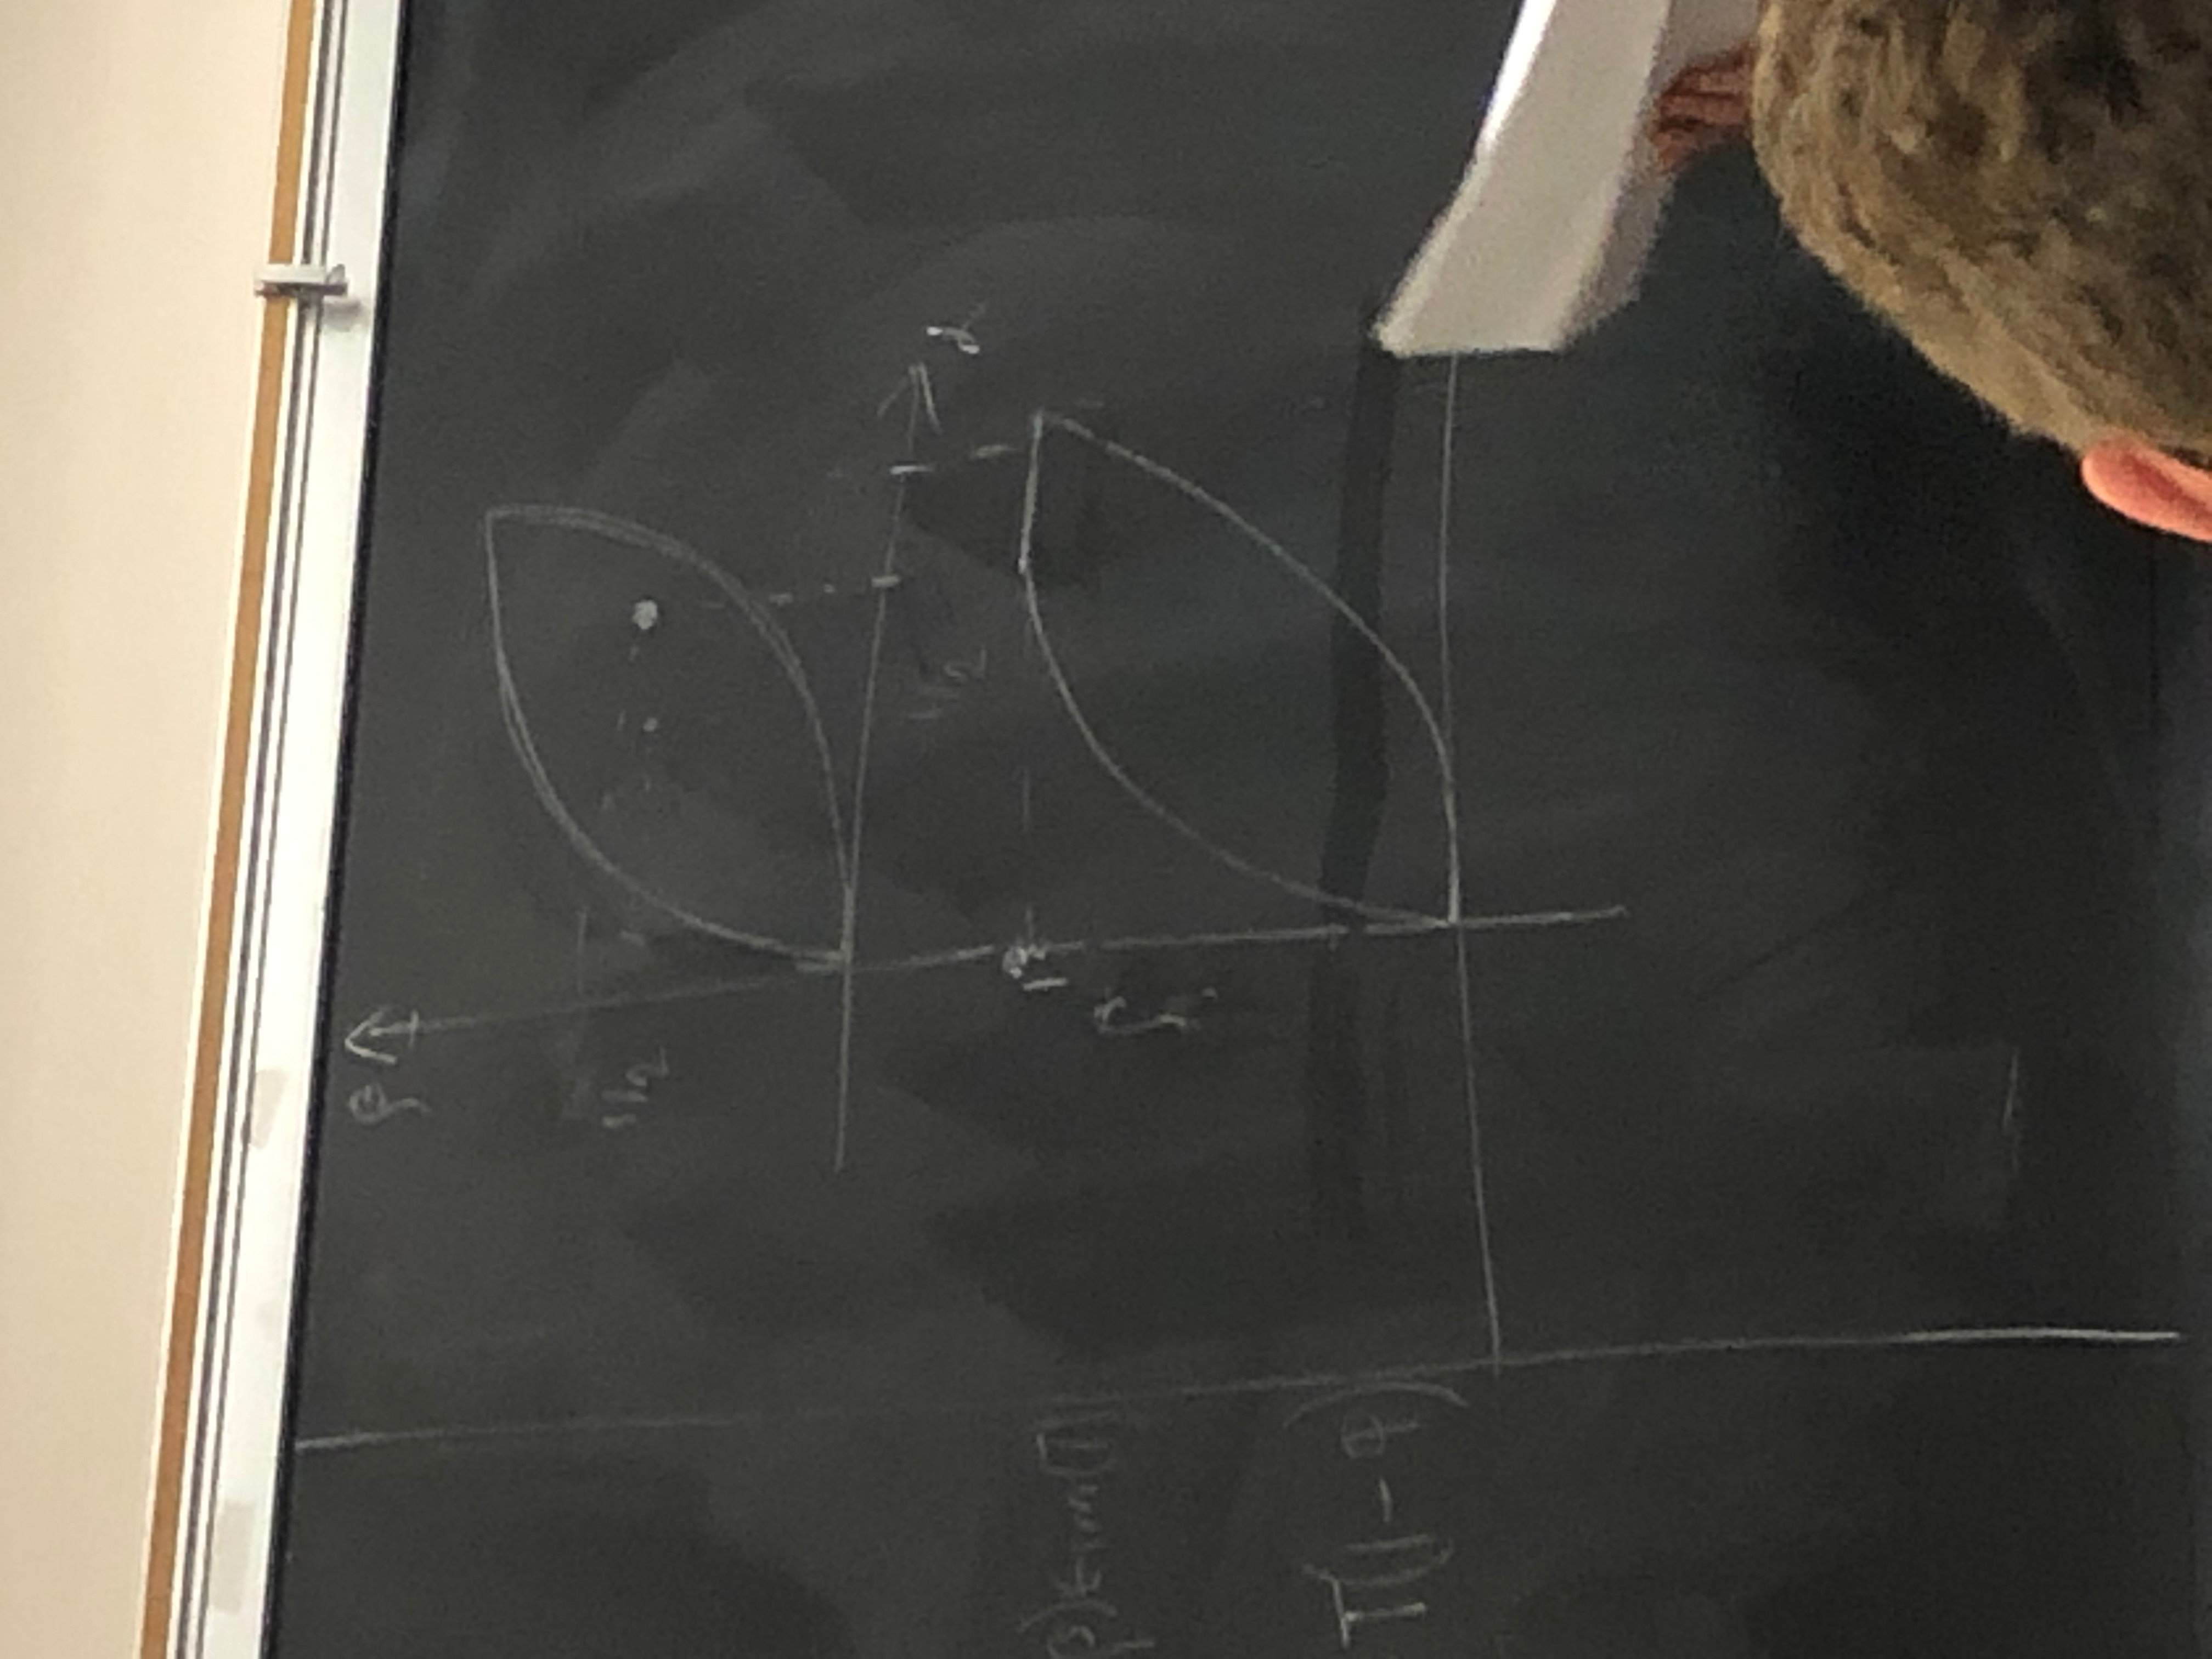
\includegraphics[scale=0.1, angle=270]{mathstats_np_set}
\caption{Sets of possible Neyman-Pearson tests; similar to Figure 3.1 in \citet{lehmann2005testing}.}
\label{mathstats.fig.np.sets}
\end{center}
\end{figure}

\begin{exercise}

\begin{enumerate}

\item Let \(\phi^*\) be the MP test of size \(\alpha\). Then \(\beta_{\phi^*} \geq \alpha\). Moreover, \(\beta_{\phi^*}\) is strictly greater than \(\alpha\) unless \(P = Q\) (Use N-P lemma, part 1). 

\item Let \(X_1, \ldots, X_n\) be i.i.d. uniform. \(H_0: X_1, \ldots, X_n \sim \operatorname{U}(0,1)\). \(H_a: X_1, \ldots, X_n \sim U(1/3, 2/3)\). Derive a UMP test of size \(\alpha\) for all values of \(\alpha\).

\end{enumerate}

\end{exercise}

\begin{solution}

\begin{enumerate}

\item

\item

\[
q(x_1, \ldots, x_n) = e^n  \prod_{i=1}^n I \{x_i \in [1/3, 2/3] ]\} = e^n I \{x_1, \ldots, x_n \in [1/3, 2/3]\}
\]

Similarly,

\[
p(x_1, \ldots, x_n) = I \{x_1, \ldots, x_n \in [0,1]\}.
\]

Note that the ratio \(q/p\) only takes on three values. By the Neyman-Pearson Lemma (Lemma \ref{mathstats.np.lem}), the most powerful test \(\phi^*\) is either

\[
\phi_1^*(x_1, \ldots, x_n) = \begin{cases}
1, & q(x_1, \ldots, x_n)/p(x_1, \ldots, x_n) = 3^n  \\
\gamma, & q(x_1, \ldots, x_n) /p(x_1, \ldots, x_n) = 0 
\end{cases}
\]

or

\[
\phi_2^*(x_1, \ldots, x_n) = \begin{cases}
\gamma, & q(x_1, \ldots, x_n)/p(x_1, \ldots, x_n) = 3^n  \\
0, & q(x_1, \ldots, x_n) /p(x_1, \ldots, x_n) = 0 
\end{cases}
\]

Now

\[
\alpha_{\phi_1^*} = \E_P \phi_1^* (X_1, \ldots, X_n) = 1 \cdot \mathbb{P}(X_1, \ldots, X_n \in [1/3, 2/3]) + \gamma \mathbb{P}(\text{at least one } X_j \text{ is outside } [1/3, 2/3])
\]

\[
= 3^{-n} + \gamma(1 - 3^{-n}) = \alpha 
\]

which has a solution for \(\gamma(\alpha)\) for \(\alpha \geq 3^{-n}\). On the other hand,

\[
\alpha_{\phi_2^*} = \E_P \phi_2^* (X_1, \ldots, X_n) = \gamma \mathbb{P}(X_1, \ldots, X_n \in [1/3, 2/3]) + 0 \cdot \mathbb{P}(\text{at least one } X_j \text{ is outside } [1/3, 2/3])
\]

\[
= \gamma 3^{-n} = \alpha
\]

which has a unique solution \(\gamma(\alpha)\) for \(\alpha \leq 3^{-n}\). So for a test with a very small \(\alpha\), you need to consider a strictly randomized test like \(\alpha_{\phi_2^*}\). 

\end{enumerate}

\end{solution}


\begin{theorem}[\textbf{Went over last time}]

We have a sequence \(X_1, \ldots, X_n\) distributed i.i.d. Last time we showed that the following hypothesis testing problem:

\[
H_0: X_1, \ldots, X_n \sim P, \qquad H_A: X_1, \ldots, X_n \sim Q
\]

with

\[
\frac{dP}{d\mu} = p, \qquad \frac{dQ}{d\mu} = q
\]

using the test

\begin{equation}\label{mathstats.np.test.def}
\phi^* (x_1, \ldots, x_n) = \begin{cases}
1, &  \prod_{i=1}^n q(x_i) > c \prod_{i=1}^n p(x_i) \\
\gamma ,&   \prod_{i=1}^n q(x_i) =  c \prod_{i=1}^n p(x_i)  \\
0, &  \prod_{i=1}^n q(x_i) <  c \prod_{i=1}^n p(x_i) 
\end{cases}
\end{equation}

is UMP of size \(\alpha = \E_P(\phi^*)(X_1, \ldots, X_n)\) (given the correct choice of \(\gamma\)).

\end{theorem}

\begin{remark}

Intuition: if the likelihood function for \(Q\) exceeds the likelihood function of \(P\) by a reasonable amount (determined by \(c\)), choose \(Q\) to be more likely than \(P\).

Also, \(\phi^*\) of this kind is referred to as a \textit{Neyman-Pearson test.}

\end{remark}

\begin{proposition}[\textbf{Math 541B Midterm Problem 2}]

The uniformly least powerful test of size \(\alpha > 0\) is

\end{proposition}

\begin{proof}

Consider again the mapping \(T: \Phi \to [0,1] \times [0,1]\) where \(\Phi\) is the set of all possible tests where \(T(\phi) = (\alpha_\phi, \beta_\phi)\) (See Figure \ref{mathstats.fig.np.sets}). Observation: \((\alpha, \beta) \in \operatorname{im}(T) \implies (1 - \alpha, 1 - \beta) \in \operatorname{im}(T)\) because if \(T(\phi) = (\alpha, \beta)\), then \( T(1 - \phi) = (1 - \alpha, 1 - \beta)\). So we have symmetry around the point \((1/2, 1/2)\). Because of this, we can see that if we find the UMP test of size \(1-\alpha\) and reverse the rejection and acceptance regions, we obtain the uniformly least powerful test of size \(\alpha\). By the Neyman-Pearson Lemma, the uniformly most powerful test of size \(\alpha\) is

\[
\phi^*(x) = \begin{cases}
1, & q(x) > c p(x) \\
0, & q(x) \leq c p(x)
\end{cases}
\]

for \(c\) chosen so that the size of the test is \(1-\alpha\). Then the uniformly least powerful test of size \(\alpha\) is 

\[
\tilde{\phi}^*(x) = \begin{cases}
1, & q(x) \leq c p(x) \\
0, & q(x) > c p(x).
\end{cases}
\]




\end{proof}

%######################
\subsection{Consistency of Neyman-Pearson Tests}
%######################

We want the test to be consistent---as we collect more data and \(n \to \infty\), errors of both types go to 0. We hope to show the consistency of Neyman-Pearson tests.

\begin{definition}[\textbf{Consistency of a hypothesis test}]

Consider the framework of the Neyman-Pearson lemma (Lemma \ref{mathstats.np.lem}, described above). A sequence of tests \(\{\phi_n\}_{n \geq 1}\), where \(\phi_n = \phi_n(x_1, \ldots, x_n)\) is \textit{consistent} if and only if

\[
\alpha_{\phi_n} = \E_P \phi_n(X_1, \ldots, X_n) \to 0, \qquad \text{and } \beta_{\phi_n} = \E_Q \phi_n(X_1, \ldots, X_n) \to 1 \qquad \text{as } n \to \infty.
\]

\end{definition}

It turns out that \(c\) grows with \(n\), and the growth condition of the size of this \(c_n\) is related to a measure of distance between \(P\) and \(Q\) (Hellinger distance). 

Recall the following definition:

\begin{definition}[\textbf{Hellinger Distance and Affinity (Definition 13.1.3 in \citet{lehmann2005testing})}]\label{mathstats.def.hel.dist}

The \textit{Hellinger distance} between probability laws \(P\) and \(Q\) is defined as 

\[
H^2(P,Q) := \int_S (\sqrt{p} - \sqrt{q})^2 \ d\mu = 2 \int_S (1 - \sqrt{pq}) d \mu = 2 - 2 \int_S \sqrt{pq} \ d\mu.
\]

(See also Section \ref{mathstats.sec.mle}.) Further,

\[
A(P,Q) := \int \sqrt{pq} \ d\mu
\]

is known as the \textit{Hellinger affinity.}

%It satisfies a nice property: if one takes the distances the distributions of two random variables \(X_1, Y_1\), \(X_2, Y_2\), \ldots, \(X_n, Y_n\), 

\end{definition}

\begin{remark}

This is a true distance---it satisfies the Triangle Inequality, \(H(P,Q) = 0\) if and only if \(P = Q\) almost everywhere.

\end{remark}

\begin{lemma}

Let \(X \sim P\) and \(Y \sim Q\). Let \(X_1, \ldots, X_n\) be i.i.d. copies of \(X\) and likewise for \(Y_1, \ldots, Y_n\), so \((X_1, \ldots, X_n) \sim P^n\) and \((Y_1, \ldots, Y_n) \sim Q^n\). Then

\[
A(P^n, Q^n) =  \left[ A(P, Q) \right]^n.
\]

\end{lemma}

\begin{proof}

%\begin{multline*}
%A(P^n, Q^n) = \int \sqrt{p(x_1, \ldots, x_n)} \sqrt{ q( x_1, \ldots, x_n) } \ d\mu \\
%= \prod_{j=1}^n \int \sqrt{p(x_i) q(x_i) \ d\mu
%\end{multline*}

\[
A(P^n, Q^n) = \int \sqrt{p(x_1, \ldots, x_n)} \sqrt{ q( x_1, \ldots, x_n) } \ d\mu^n 
= \prod_{j=1}^n \int \sqrt{p(x_j) q(x_j)} \ d\mu_j=  \left[ A(P, Q) \right]^n.
\]

\end{proof}

\begin{theorem}[\textbf{Consistency of Neyman-Pearson tests}]

Assume that \(\rho := A(P,Q) < 1\). Then take any sequence \(\{c_n\} \subset \mathbb{R}_+\) such that 

\begin{equation}\label{mathstats.cons.np.a}
\rho^{2n} \ll c_n \ll \rho^{-2n}.
\end{equation}

Then any sequence \(\{\phi_n\}_{n \geq 1}\) of Neyman-Pearson tests corresponding to \(\{c_n\}_{n \geq 1}\) is consistent. 

\end{theorem}

\begin{proof}

First, we will show that \(\alpha_{\phi_n} \to 0\) under these conditions. Recall the definition of \(\phi\) from (\ref{mathstats.np.test.def}). 

\begin{multline*}
\alpha_{\phi_n}  = \int \phi(x_1, \ldots, x_n) p(x_1, \ldots, x_n) \ d \mu^n
 \\
\leq \int I  \left\{  \frac{ \prod_{i=1}^n q(x_i)}{ \prod_{i=1}^n p(x_i)} \geq c_n \right\} p(x_1) \cdots p(x_n)  \ d\mu^n =  \int I  \left\{  \frac{ \prod_{i=1}^n q(x_i)}{c_n \prod_{i=1}^n p(x_i)} \geq 1 \right\} p(x_1) \cdots p(x_n)  \ d\mu^n 
\\
\leq \int  \sqrt{\frac{ q(x_1) \cdots q(x_n)}{c_n p(x_1) \cdots p(x_n) } }  p(x_1) \cdots p(x_n) \ d \mu^n 
\\
= \frac{1}{\sqrt{c_n}} \int \sqrt{q(x_1) \cdots q(x_n)} \sqrt{ p(x_1) \cdots p(x_n)} d \mu^n = \rho^n c_n^{-1/2}  \to 0 \text{ as } n \to \infty.
\end{multline*}



(The second inequality follows because when the indicator equals 0 the square root term is greater than or equal to 0 but when the indicator equals 1 the square root term is greater than or equal to 1. The last step follows by assumption of the lemma.)

Now consider the Type II error \(1 - \beta_{\phi_n}\). 

\begin{multline*}
1 - \beta_{\phi_n} = \int [1 - \phi(x_1, \ldots, x_n)]q(x_1) \cdots q(x_n) \ d\mu^n \\
\leq \int I \left\{q(x_1) \cdots q(x_n) \leq c p(x_1) \cdots p(x_n) \right\} q(x_1) \cdots q(x_n) \ d\mu^n \\
\leq  \int  \sqrt{\frac{ p(x_1) \cdots p(x_n)}{q(x_1) \cdots q(x_n) }  \cdot c_n  }  \cdot q(x_1) \cdots q(x_n) \ d \mu^n  \\
= \sqrt{c_n} A(P^n, Q^n) = c-n^{1/2} \rho^n \to 0 \text{ as } n \to \infty
\end{multline*}

\end{proof}

\begin{remark}

Intuition: \( A(P,Q) < 1 \iff  H(P, Q) > 0 \iff P \neq Q\). Also, \(a_n \ll b_n \iff a_n = o(b_n)\), and \(a_n \gg b_n \iff b_n \ll a_n\). Almost all reasonable sequences satisfy (\ref{mathstats.cons.np.a})---this range is very large. 

Basically, this theorem says the Type I and Type II errors converge to 0 geometrically fast (as \(\rho^n\)) if \(P\) and \(Q\) are not too close together.

\end{remark}

\begin{proposition}[\textbf{Stats 100B Homework problem}] Let \(Y_1, Y_2, \ldots, Y_n\) be the outcomes of \(n\) independent Bernoulli trials. Then by the Neyman-Pearson lemma (Lemma \ref{mathstats.np.lem}), the best critical region for testing

\[
H_0: p = p_0 \ \ \ \ \ \ \ H_a: p > p_0
\]

is

\[
\frac{y}{n} = \frac{1}{n}\sum Y_i  > \frac{\log(K) + n \log \bigg( \frac{1 - p_a}{1 - p_0} \bigg)}{n\log \bigg( \frac{p_0(1 - p_a)}{p_a(1 - p_0)} \bigg)}.
\]

\end{proposition}

\begin{proof}

\[
\Pr(\sum Y_i = y) = {n \choose y}p^y(1-p)^{n-y}
\]

Using the Neyman-Pearson lemma (let \(p_a\) be some particular value of \(p > p_0\)):

\[
\frac{L(p_0)}{L(p_a)} = \frac{{n \choose y}p_0^y(1-p_0)^{n-y}}{{n \choose y}p_a^y(1-p_a)^{n-y}} < K
\]

\[
\bigg( \frac{p_0}{p_a} \bigg) ^y   \bigg( \frac{1 - p_0}{1 - p_a} \bigg)^{n} \bigg( \frac{1 - p_0}{1 - p_a} \bigg)^{-y}  < K
\]

\[
\bigg( \frac{p_0(1 - p_a)}{p_a(1 - p_0)} \bigg) ^y  < K  \bigg( \frac{1 - p_a}{1 - p_0} \bigg)^{n} 
\]

\[
y \log \bigg( \frac{p_0(1 - p_a)}{p_a(1 - p_0)} \bigg) < \log(K) + n \log \bigg( \frac{1 - p_a}{1 - p_0} \bigg)
\]

Aside:

\[
\frac{p_0(1 - p_a)}{p_a(1 - p_0)} = \frac{p_0 - p_0 p_a}{p_a - p_0 p_a} < 1
\]

since by assumption \(p_a > p_0\). Therefore \( \log \bigg( \frac{p_0(1 - p_a)}{p_a(1 - p_0)} \bigg) < 0 \). So we have

\[
\frac{y}{n} = \frac{1}{n}\sum Y_i  > \frac{\log(K) + n \log \bigg( \frac{1 - p_a}{1 - p_0} \bigg)}{n\log \bigg( \frac{p_0(1 - p_a)}{p_a(1 - p_0)} \bigg)}
\]

as the form for our critical region.

\end{proof}

%######################
\subsection{Composite Hypothesis Testing}
%######################

% !!Please put ########## above and below the section/subsection name for better readability (as the section name above)

% Some comments regarding LaTeX typesetting:
% (1) Please use \[ math here  \] instead of $$ math here $$ for displayed equations, and separate them from the main text: 
% for example, 
% \[
% \sqrt{x^2} = | x |
% \]
% (2) Please use \begin{multline} \end{multline} for numbered multiline equations, or \begin{multline*} \end{multline*} for non-numbered equations ( \\ symbol is used for line breaks), and \begin{equation} \end{equation} for numbered one-line equations
% (3) use \l and \r (shortcuts for \left and \right) for automatic bracket resizing, for example 
% $\l( \int\limits_0^\infty f(x) dx \r)^2 \leq \int\limits_0^infty f^2(x) dx$
% To make the code readable, try to keep lines short (by pressing "enter" in your editor). 


We will start with one-dimensional family (one parameter), then expand to multiple parameters using tricks based on conditioning and using the principles of sufficiency and completeness.

\begin{definition}[\textbf{Composite Hypothesis Test}]



Assume we have a statistical model \(\{P_\theta, \theta \in \Theta\}\). Let \(\Theta_0, \Theta_1 \subset \Theta\) be such that \(\Theta_0 \cap \Theta_1 = \emptyset\) and \(\Theta_0 \cup \Theta_1 = \Theta\). Assume \( X \sim P_\theta \text{ for some } \theta \in \Theta\) (where \(X\) may be multivariate). We would like to test the hypotheses

\[
H_0:  \theta \in \Theta_0, \qquad H_a: \theta \in \Theta_1.
\]

Such a test is a \textit{composite hypothesis test}.

\end{definition}

The Neyman-Pearson Lemma (Lemma \ref{mathstats.np.lem}) does not directly apply to composite hypothesis tests, but it turns out we can use the Neyman-Pearson lemma to prove some results about some composite hypothesis tests under some circumstances.

\begin{definition}[\textbf{Power function; definition 8.3.1 in \citet{CaseBerg:01}}]

The \textit{power function} of a test \(\phi\) is defined as

\[
\beta_\phi(\theta) := \E_\theta \phi(X).
\]

\end{definition}

\begin{remark}

For \(\theta \in \Theta_0\), \(\beta_\phi(\theta)\) is the probability of a Type 1 error; for \(\theta \in \Theta_1\), \(\beta_\phi(\theta)\) is the power of \(\phi\).

\end{remark}

\begin{definition}[\textbf{Test size; definition 8.3.6 in \citet{CaseBerg:01}}]

The test \(\phi\) is of \textit{size} \(\alpha\) if and only if 

\[
\sup_{\theta \in \Theta_0} \beta_\phi(\theta) \leq \alpha.
\]

\end{definition}

\begin{definition}[\textbf{Uniformly most powerful test; definition 8.3.11 in \citet{CaseBerg:01}}]

\(\phi^*\) is the \textit{uniformly most powerful test} of size \(\alpha\) if \(\phi^*\) is of size \(\alpha\) and \(\beta_{\phi^*}(\theta) \geq \beta_\phi(\theta)\) for any other test \(\phi\) of size \(\alpha\) for all \(\theta \in \Theta_1\).

\end{definition}

We will be interested in families with \textit{monotone likelihood ratios}. (Note: for the rest of the class today, \(\Theta = [a, b] \subseteq \mathbb{R}\) with \(a, b \in [-\infty, \infty]\)). 

\begin{definition}[\textbf{Monotone likelihood ratio; definition 8.3.16 in \citet{CaseBerg:01}}]

Let \(T(X)\) be a statistic. Consider \(\Theta \subseteq \mathbb{R}\) as a segment on the real line. We say that the family of pdfs \(\{p_\theta, \theta \in \Theta\}\) has a \textit{monotone likelihood ratio (MLR)} with respect to \(T(x)\) if and only if for any \(\theta' > \theta''\), 

\[
\frac{p_{\theta'}(x)}{p_{\theta''}(x)} = \psi_{\theta', \theta''}(T(x))
\]

where \(\psi_{\theta', \theta''}(\cdot)\) is non-decreasing. (That it is non-decreasing is without loss of generality; in the case that \(\psi\) is non-increasing, simply replace \(T(x)\) with \(-T(x)\) to achieve a non-decreasing \(\psi\)).

\end{definition}

\begin{example}

Let \(X \sim \operatorname{Poisson}(\lambda)\), so 

\[
p_\lambda(x) =  \frac{e^{-\lambda} \lambda^x}{x!}, \qquad x \in \mathbb{Z}_+.
\]

Then  \(\{ \operatorname{Poisson}(\lambda), \lambda \in \mathbb{R}_+\}\) has a monotone likelihood ratio with respect to \(T(x) =x\) by the following argument. Take \(\lambda' > \lambda ''\). Then 

\[
\frac{e^{- \lambda '} (\lambda')^x x! }{x! e^{-\lambda ''} (\lambda'')^x }=  e^{-(\lambda' - \lambda'')} \left( \frac{ \lambda'}{\lambda ''} \right)^x
\]

and

\[
\psi_{\lambda', \lambda''}(x) = e^{-(\lambda' - \lambda'')} \left( \frac{ \lambda'}{\lambda ''} \right)^x
\]

is non-decreasing. 

\end{example}

\begin{theorem}[\textbf{Karlin-Rubin; similar to Theorem 8.3.17 in \citet{CaseBerg:01}, Theorem 3.4.1 in \citet{lehmann2005testing}}]\label{mathstasts.thm.karlin.rubin}

Assume \(\{p_\theta, \theta \in[a,b]\}\) has a monotone likelihood ratio with respect to some sufficient statistic for \(\theta \in \mathbb{R}\), \(T(x)\). Suppose we want to test

\[
H_0: \theta \leq \theta_0, \qquad H_a: \theta > \theta_0.
\]

Then there exists \(c \geq 0\) and \(\gamma \in [0,1]\) such that 

\[
\phi^*(x) = \begin{cases}
1, &  T(x) >c \\
\gamma, & T(x) = c \\
0, & T(x) < c
\end{cases}
\]

is the uniformly most powerful test of size \(\alpha\). (In other words, the UMP test will always be of this form.)

\end{theorem}

\begin{proof}

We will show that this is the uniformly most powerful test over the larger family of tests that satisfy \(\E_{\theta_0} \phi(x) = \alpha\) (\(\beta_\phi(\theta_0) \leq \alpha\)), which contains tests of size \(\alpha\). So if we can find the UMP test for this larger family (and it is a test of size \(\alpha\)), then that is also the UMP test for test of size \(\alpha\) (satisfying \(\sup_{\theta \in \Theta_0} \beta_\phi(\theta) \leq \alpha\)).

First note that we can always find \(c\) and \(\gamma\) such that 

\[
\E_{\theta_0}(\phi^*(x) = \alpha.
\]

Define \(F(c) := \mathbb{P}_{\theta_0}( \{x: T(x) \leq x\})\). Note that

\[
\E_{\theta_0}\psi^*(x) = F(c) + \gamma[F(c) - F(c^+)]
\]

where \(F(c) - F(c^+)\) is the size of the jump. (The proof of this claim is an exercise.) 

Next, take \(\theta' > \theta_0\) and consider the simple hypothesis test

\[
H_{0}': \theta = \theta_0, \qquad H_a': \theta = \theta'.
\]

By the Neyman-Pearson Lemma (Lemma \ref{mathstats.np.lem}), the most powerful test for this is 

\[
\phi'(x) = \begin{cases}
1, & p_{\theta'}(x) > c' p_{\theta_0}(x) \\
\gamma', &  p_{\theta'}(x) = c' p_{\theta_0}(x) \\
0, & p_{\theta'}(x) < c' p_{\theta_0}(x) 
\end{cases} \iff 
\phi'(x) = \begin{cases}
1, & p_{\theta'}(x)/  p_{\theta_0}(x) > c' \\
\gamma', &  p_{\theta'}(x)/  p_{\theta_0}(x) = c' \\
0, & p_{\theta'}(x)/ p_{\theta_0}(x)  < c' 
\end{cases}
\]

But since \( p_{\theta'}(x)/  p_{\theta_0}(x)  = \psi(T(x))\), by the assumption of the monotone likelihood ratio property,

\[
\frac{p_{\theta'}(x)}{  p_{\theta_0}(x)} > c' \iff T(x) > \psi^{-1}(c').
\]

Set \(\psi^{-1}(c') = c\) and \(\psi^{-1}(\gamma') = \gamma\) (using the values of \(\gamma\) and \(c\) from earlier in the proof). Then we have

\[
\phi'(x) = \begin{cases}
1, & T(x) > c \\
\gamma', & T(x) = c \\
0, & T(x) < c
\end{cases}
\]

as desired. (Moreover, \(c\) and \(\gamma\) are uniquely determined by \(\E_{\theta_0}(\phi^*) = \alpha\). Note that \(\theta'\) does not appear anywhere in this test. Since \(\theta'\) was arbitrary, the proof is almost complete.

The final argument is to show that this test has size \(\alpha\). Namely, we must show

\[
\sup_{\theta \leq \theta_0} \beta_{\phi^*}(\theta) = \sup_{\theta \leq \theta_0} \E_\theta \phi^*(x) \leq \alpha.
\]

It is sufficient to show that \(\beta_{\phi^*}(\theta)\) is monotone. Take \(\theta_1 < \theta_2\). Then by the Neyman-Pearson Lemma (Lemma \ref{mathstats.np.lem}), we know that \(\phi^*\) is the UMP test for testing

\[
H_0'':  \theta = \theta_1 \qquad H_a'':  \theta = \theta_2
\]

of size \(\beta_{\phi^*}(\theta)\). Since it is the most powerful test, its power \(\E_{\theta_2} \phi^*(x)\) is at least as powerful than the test which is identically equal to \(\beta_{\phi^*}(\theta)\); that is, \(\E_{\theta_2}(\phi^*(x) \geq \E_{\theta_1}(\phi^**(x)\).

%this will be done in the next lecture. From there we can conclude that this is the uniformly most powerful test of size \(\alpha\).


\end{proof}


\begin{example}

\(X_1, \ldots, X_n \sim \mathcal{N}(\mu, 1)\). Test \(H_0: \mu \leq 0\) against \(H_1: \mu > 0\). Find the UMP test.

\end{example}

\begin{solution}

Take \(\mu_1 > \mu_2\). Then 

\begin{multline*}
\frac{ p_{\mu_1}(x_1, \ldots, x_n)}{ p_{\mu_2}(x_1, \ldots, x_n)} = \exp \left\{ - \frac{1}{2} \left[ \sum_{i=1}^n (x_i - \mu_1)^2 -  \sum_{i=1}^n (x_i - \mu_2)^2  \right]\right\}
\\ = \exp \left\{ - \frac{1}{2} \left[ n(\mu_1^2 - \mu_2^2) + (\mu_1 - \mu_2) \sum_{i=1}^n x_i \right]\right\}
\end{multline*} 

This is an increasing function with respect to \(T(x_1, \ldots, x_n) = \sum_{i=1}^n x_i\). Therefore by Theorem \ref{mathstasts.thm.karlin.rubin}, we have that the UMP test is 

\begin{equation}\label{mathstats.kr.ex.1}
\phi(x_1, \ldots, x_n) = \begin{cases}
1, & \sum_{i=1}^n x_i \geq c_\alpha \\
0, & \sum_{i=1}^n x_i < c_\alpha
\end{cases} = \begin{cases}
1, & n^{-1/2} \sum_{i=1}^n x_i \geq c_\alpha' \\
0, & n^{-1/2} \sum_{i=1}^n x_i < c_\alpha'
\end{cases}
\end{equation}

Note that 

\[
\E_{\mu=0} \phi(X_1, \ldots, X_n) = \alpha \iff  \mathbb{P} \left( \frac{1}{\sqrt{n}} \sum_{i=1}^n X_i \geq c_\alpha' \right) = \alpha
\]

and \(n^{-1/2} \sum_{i=1}^n X_i  \sim \mathcal{N}(0,1)\). Therefore \(c_\alpha' = z_{1- \alpha}\) (the \(1-\alpha\) quantile of a standard Gaussian distribution). Substituting this into (\ref{mathstats.kr.ex.1}) defines the UMP test.

\end{solution}

\begin{remark}

The Karlin-Rubin Theorem (Theorem \ref{mathstasts.thm.karlin.rubin}) still applies if the inequalities in the hypothesis test are reversed.

\end{remark}

\begin{example}

\(X_1, \ldots, X_n \sim \mathcal{N}(\mu, 1)\). Test \(H_0: \mu \in [0,1]\) against \(H_1: \mu < 0 \cup \mu > 1\). Does there exist a UMP test?

\end{example}

\begin{solution}

No. Consider \(H_0': \mu \in [0,1], H_a': \mu > 1\) and \(H_0'': \mu \in [0,1], H_a'': \mu < 1\). If the UMP test for our test exists, it must be identical to the UMP tests for both of these tests (since it would have to be UMP over ever \(\theta\)). By Theorem \ref{mathstasts.thm.karlin.rubin}, the UMP test in the first case is 

\[
\phi'(x_1, \ldots, x_n) = \begin{cases}
1, & \sum_{i=1}^n x_i \geq c \\
0, & \sum_{i=1}^n x_i < c.
\end{cases}
\]

The UMP test in the second case is 

\[
\phi'(x_1, \ldots, x_n) = \begin{cases}
1, & \sum_{i=1}^n x_i \leq c \\
0, & \sum_{i=1}^n x_i > c.
\end{cases}
\]

Since these tests are not identical, there is no UMP test for our test.

\end{solution}

\begin{theorem}[\textbf{Generalized Neyman-Pearson Lemma, Theorem 3.6.1 in \citet{lehmann2005testing}}]\label{mathstats.lem.np.gen}

Assume that \(f_0, f_1, \ldots, f_n: \mathbb{R}^d \to \mathbb{R}\) such that 

\[
\int |f_j| \ d\mu < \infty, \qquad j \in \{0, \ldots, N\}.
\]

\begin{enumerate}

\item

We seek to maximize the \(\int \phi  f_0 \ d\mu \) over all tests \(\phi\) subject to \(\int \phi f_j \ d\mu = \alpha_j, j \in \{1, \ldots, N\}\). 

\item

We seek to maximize the \(\int \phi  f_0 \ d\mu \) over all tests \(\phi\) subject to \(\int \phi f_j \ d\mu \leq \alpha_j, j \in \{1, \ldots, N\}\). 

\end{enumerate}

Suppose there exists \(k_1, \ldots, k_N\) such that 

\[
\phi^* = \begin{cases}
1, & f_0(x) > k_1 f_1(x) + \ldots + k_N f_N(x) \\
0, & f_0(x) < k_1 f_1(x) + \ldots + k_N f_N(x) 
\end{cases}
\]

satisfies \(\int \phi^* f_j \ d\mu = \alpha_j, j \in \{1, \ldots, N\} \). Then \(\phi^*\) solves the first problem. Moreover, if \(k_1, \ldots, k_N \geq 0\), then \(\phi^*\) also solves the second problem.

\end{theorem}

\begin{example}[\textbf{Like Theorem 3.7.1 in \citet{lehmann2005testing}}]\label{mathstats.gnp.ex.prob}

\(\{P_\theta, \theta \in \Theta\}\). \(H_0: \theta \in [\theta_1, \theta_2]\). \(H_a: \theta \notin [\theta_1, \theta_2]\). We have 

\[
p_\theta(x) =  \frac{1}{c(\theta)} e^{\theta T(x)}
\]

(one-parameter exponential family). Find the UMP unbiased test.

\end{example}

\begin{solution}

For the test to be unbiased, the Type I error rate has to be less than or equal to \(\alpha\) (for all \(\theta \in [\theta_1, \theta_2]\)) and the power has to be greater than or equal to \(\alpha\) (for all \(\theta\) in the rejection region). We will use the Generalized Neyman-Pearson Lemma (Theorem \ref{mathstats.lem.np.gen}) to show the solution is of the form

\[
\phi^*(x) = \begin{cases}
1, & T(x) < c_1 \text{ or } T(x) > c_2 \\
\gamma_1, & T(x) = c_1 \\
\gamma_2, & T(x) = c_2 \\
0, & T(x) \in (c_1, c_2)
\end{cases}
\]

such that \(\E_{\theta_1} \phi^*(X) = \E_{\theta_2} \phi^*(X) = \alpha\). By the Generalized Neyman-Pearson Lemma, we look for the solution in the form

\begin{multline}\label{mathstats.np.gen.ex.a}
\tilde{\phi}(x) = \begin{cases}
1, & p_{\theta'}(x) > k_1  p_{\theta_1}(x) + k_2 p_{\theta_2}(x) \\
0, & p_{\theta'}(x) < k_1  p_{\theta_1}(x) + k_2 p_{\theta_2}(x).
\end{cases}
= \begin{cases}
1, & \frac{1}{c(\theta')} e^{\theta' T(x)}> k_1  \frac{1}{c(\theta_1)} e^{\theta_1 T(x)}+ k_2  \frac{1}{c(\theta_2)} e^{\theta_1 T(x)}\\
0, & \frac{1}{c(\theta')} e^{\theta' T(x)}< k_1  \frac{1}{c(\theta_1)} e^{\theta_1 T(x)} + k_2 \frac{1}{c(\theta_2)} e^{\theta_1 T(x)}.
\end{cases}
\\ = \begin{cases}
1, & 1 > \tilde{k}_1e^{(\theta_1 - \theta') T(x)} + \tilde{k}_2e^{(\theta_2  - \theta') T(x)} \\
0, & 1 < \tilde{k}_1e^{(\theta_1 - \theta') T(x)} + \tilde{k}_2e^{(\theta_2  - \theta') T(x)}.
\end{cases}
\end{multline}

Let's analyze the inequality \(g(t) < 1\) where 

\[
g(t) =  \tilde{k}_1e^{a_1 t } + \tilde{k}_2e^{a_2 t}
\]

with \(a_1 = \theta_1 - \theta' > 0, a_2 = \theta_2 - \theta' > 0, a_1 < a_2\). Consider the second case.

\begin{enumerate}[(a)]

\item \(\tilde{k}_1 > 0, \tilde{k}_2 > 0 \implies g(t)\) is increasing. \(g(t) < 1 \iff t< c\) for some \(c \in \mathbb{R}\). From the Karlin-Rubin Theorem, in this case \(\beta_{\tilde{\phi}}(\theta) \) is monotone. But this is impossible, as we require \(\beta_{\tilde{\phi}}(\theta_1) =  \beta_{\tilde{\phi}}(\theta_2)\).

\item \(\tilde{k}_1 < 0, \tilde{k}_2 < 0 \implies g(t) < 1\). Examining (\ref{mathstats.np.gen.ex.a}) shows that in this case \(\tilde{\phi}(x) = 1\) for all \(x\) (so \(\tilde{\phi}\) always rejects), so we can't have controlled Type I error.

\item \(\tilde{k}_1 < 0, \tilde{k}_2 > 0\). In this case, \(g'(t) = \tilde{k}_1 a_1 e^{a_1 t} + \tilde{k}_2 a_2 e^{a_2 t}\). Then \(g'(t) = 0\) has a unique solution (see Figure \ref{mathstats_gnp_ex_fig}), and \(g(t) < 1 \iff t \in (c_1, c_2)\) (rejection only happens in this bounded interval). But this can't be a UMP unbiased test because the power function of this test is less than a constant test. We should have high power as our test statistic goes off to infinity or negative infinity, but examining (\ref{mathstats.np.gen.ex.a}), we see that \(\tilde{\phi}(x)= 0\) as \(T(x) \to \infty\) or \(- \infty\).

\begin{figure}[htbp]
\begin{center}
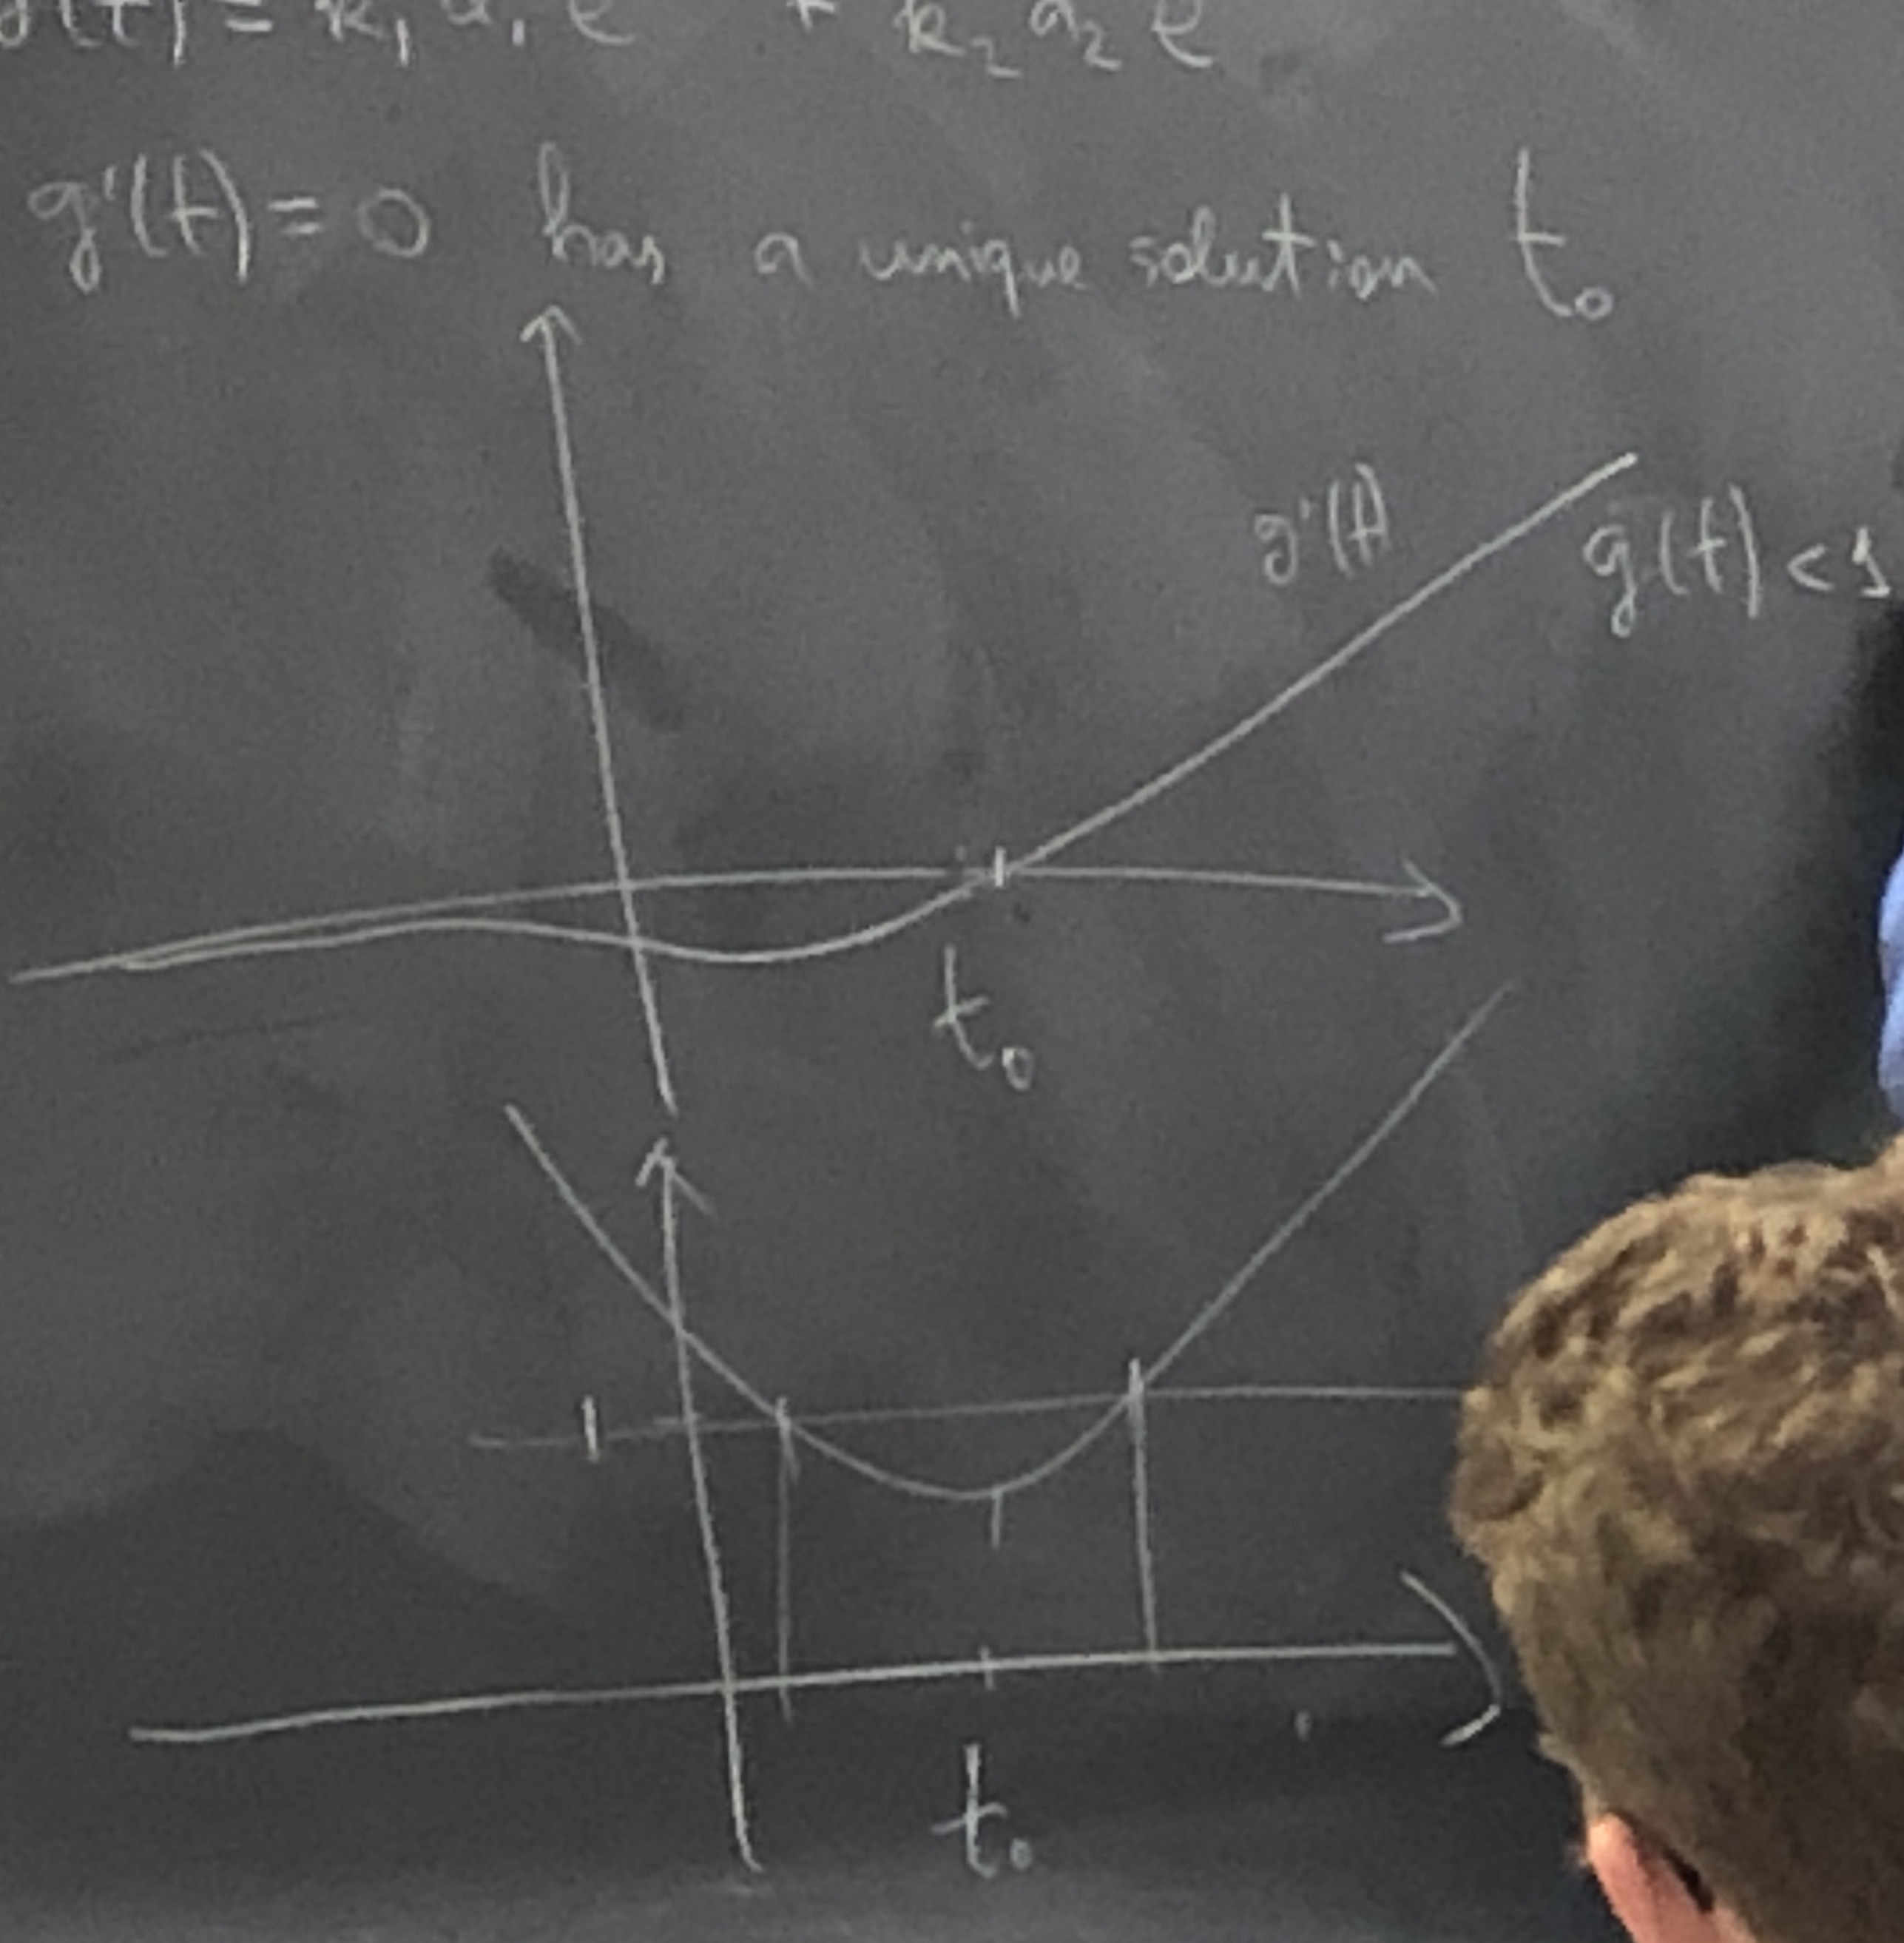
\includegraphics[scale=0.1]{mathstats_gnp_ex}
\caption{Figure for Example \ref{mathstats.gnp.ex.prob}, case (c). This can't be the UMP unbiased test because our power is approaches 0 the further away we get from this narrow interval (we accept the null hypothesis when this function is more than 1).}
\label{mathstats_gnp_ex_fig}
\end{center}
\end{figure}

\item \(\tilde{k}_1 > 0, \tilde{k}_2 < 0\). Then \(g'(t)\) has a unique zero (see Figure \ref{mathstats_gnp_ex_fig_2}), and \(g(t) < 1 \iff t \in (c_1, c_2)\) which gives us the form of the test that we were looking for (we always accept the null hypothesis when this function is more than 1 and reject it when it is less than 1).

\begin{figure}[htbp]
\begin{center}
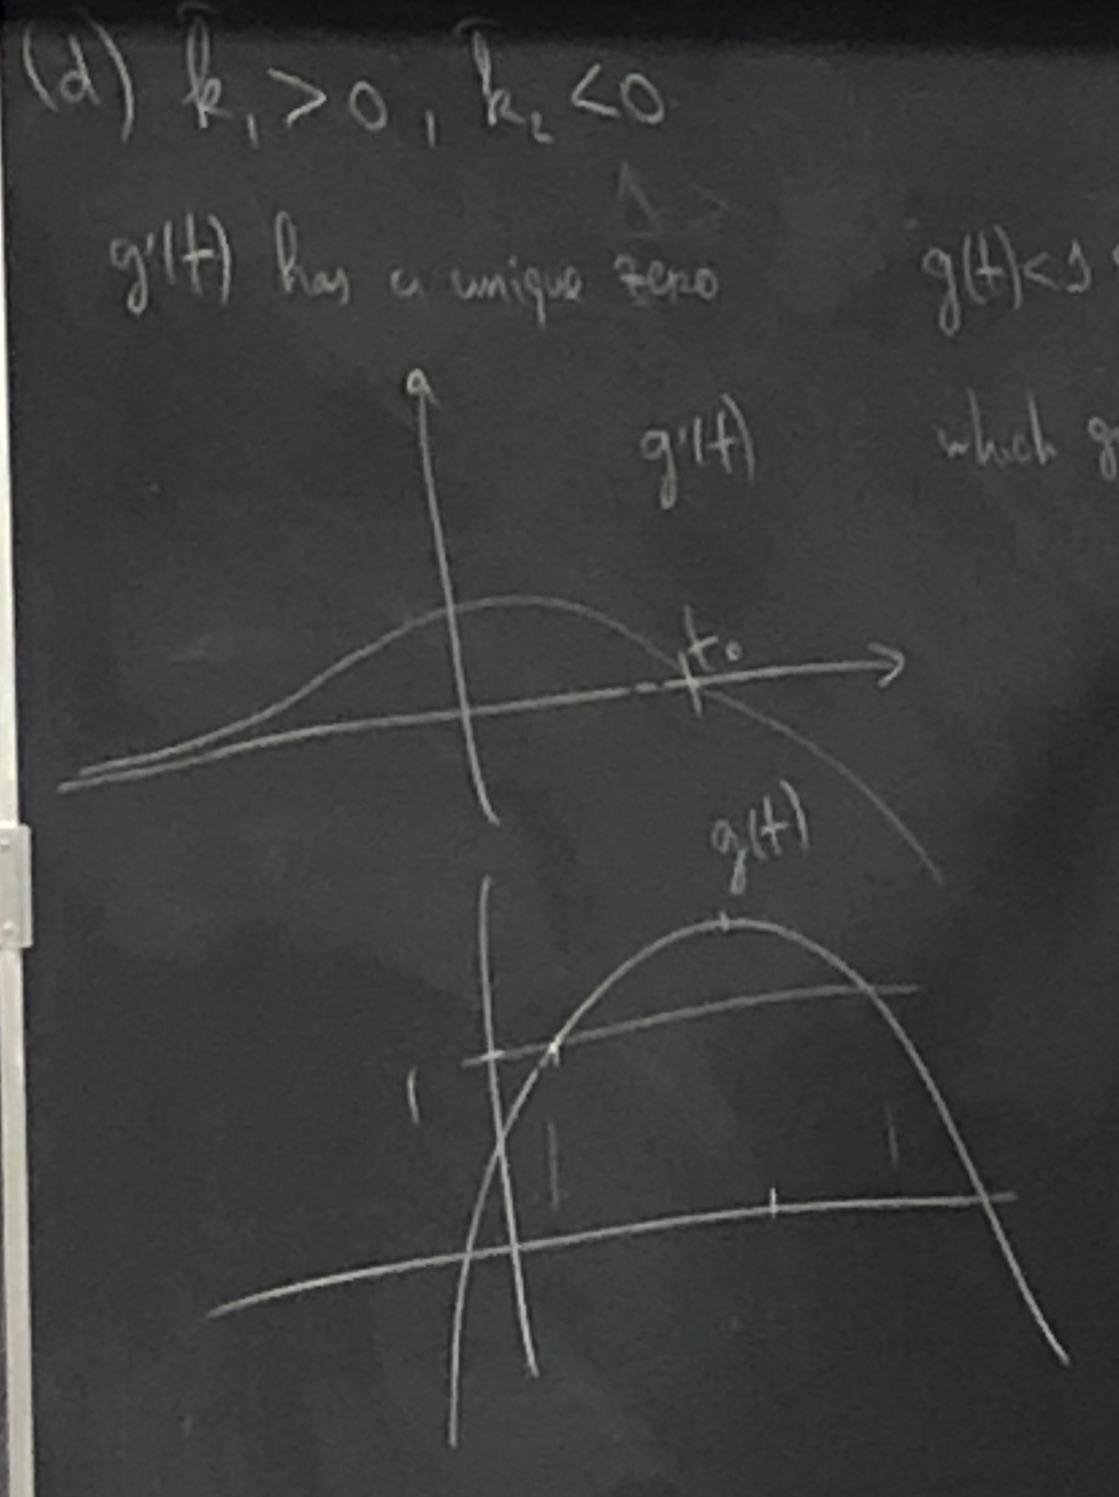
\includegraphics[scale=0.2]{mathstats_gnp_ex_2}
\caption{Second figure for Example \ref{mathstats.gnp.ex.prob}, case (d). This is the form of the UMP unbiased test.}
\label{mathstats_gnp_ex_fig_2}
\end{center}
\end{figure}


\end{enumerate}

It remains to show that \(\beta_{\phi^*}(\theta) \leq \alpha\) for all \(\theta \in [\theta_1, \theta_2]\) (the power function appears as in Figure \ref{mathstats_gnp_ex_fig_3}). We can show this in one of two ways.

\begin{enumerate}[(a)]

\item \(\beta_{\phi^*}'(\theta) = 0\) has a unique solution (then by a similar argument to that used in parts (c) and (d) of the previous part, the power function will have the form we want).

\item Lemma: the test \(\phi^*\) minimizes the power at any \(\theta' \in (\theta_1, \theta_2)\) among all SOB tests.  (proof: exercise, similar mechanics to this).

\end{enumerate}

\begin{remark}

SOB means "similar on the boundary." Recall that the definition of unbiasedness for a hypothesis test is that for a null hypothesis region \(\Omega_H\) and an alternative hypothesis region \(\Omega_k\), we have

\[
\E_{\theta_0} \phi(X) \leq \alpha \qquad \forall \theta_0 \in \Theta_H, \qquad \E_{\theta_a} \phi(X) \geq \alpha \qquad \forall \theta_a \in \Theta_K.
\]

If the power function \(\beta_\phi(\theta) := \E_\theta \phi(X)\) is a continuous function of \(\theta\), unbiasedness implies 

\begin{equation}\label{mathstats.sob.cond}
\beta_\phi(\theta) = \alpha \ \forall \theta \in \Theta_B,
\end{equation}

 where \(\Theta_B\) is the common boundary of \(\Theta_H\) and \(\Theta_K\); that is, the set of points \(\theta\) that are points or limit points of both \(\Omega_H\) and \(\Omega_K\). See Section 4.1 of \citet{lehmann2005testing} and Lemma \ref{mathstats.lehman.rom.lem.4.1.1.ump.unbiased}.
 
  \end{remark}
 
 
 \begin{definition}[\textbf{``Similar on the boundary" tests}]\label{mathstats.def.sob}
 Tests satisfying (\ref{mathstats.sob.cond}) are said to be \textbf{similar on the boundary}. 

\end{definition}


We can prove this in a way similar to Theorem 3.6.1 in \citet{lehmann2005testing}, although the proof is a little different.

\begin{figure}[htbp]
\begin{center}
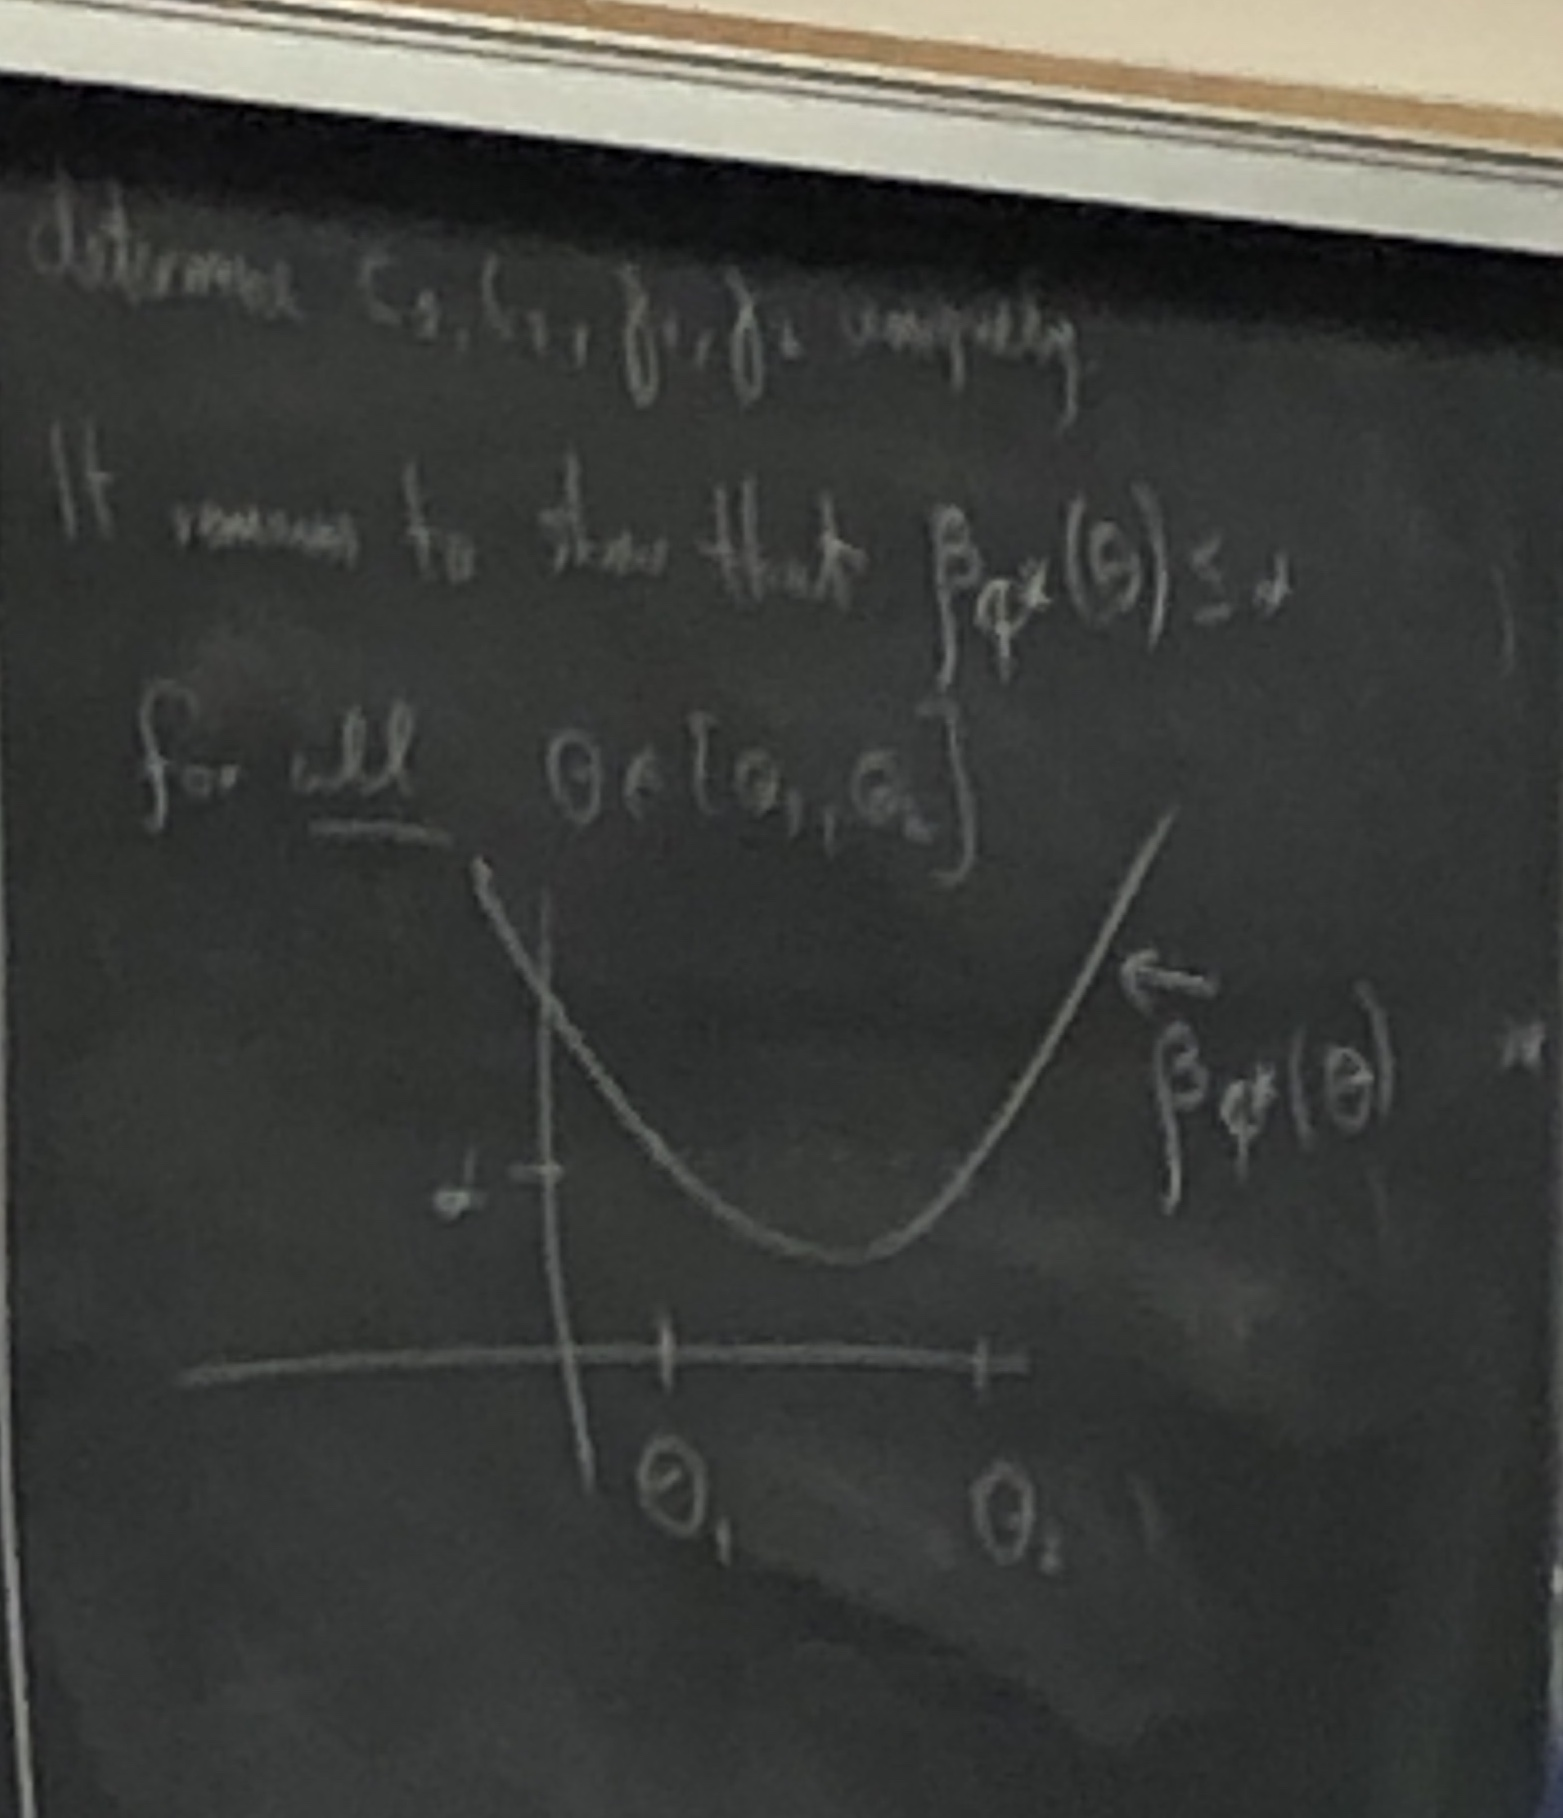
\includegraphics[scale=0.15]{mathstats_gnp_ex_3}
\caption{Third figure for Example \ref{mathstats.gnp.ex.prob}, the desired form of a power function for our selected test.}
\label{mathstats_gnp_ex_fig_3}
\end{center}
\end{figure}

\end{solution}

\begin{theorem}[\textbf{Theorem 3.7.1 in \citet{lehmann2005testing}}]

The most powerful unbiased test for a one-parameter exponential family is 

\[
\phi^*(x) = \begin{cases}
1, & T(x) < c_1 \text{ or } T(x) > c_2 \\
\gamma_1, & T(x) = c_1 \\
\gamma_2, & T(x) = c_2 \\
0, & T(x) \in (c_1, c_2)
\end{cases}
\]

such that 

\begin{enumerate}[(a)]

\item \(\E_{\theta_0}(\phi^*(X) = \alpha\).

\item \( \left. \deriv{}{\theta} \beta_{\phi^*}(\theta) \right|_{\theta = \theta_0} = 0\)  (\(\E_{\theta_0} T(X) \phi^*(X) = \alpha \E_{\theta_0} T(X)\)).

\end{enumerate}



\end{theorem}

\begin{proof}[Proof of constraint (b).]  For any unbiased test \(\phi\) of size \(\alpha\),



\[
p_\theta(x) = \frac{1}{c(\theta)} e^{\theta T(x)} = \tilde{c}(\theta)e^{\theta T(x)}
\]

(letting \( \tilde{c}(\theta) =  \frac{1}{c(\theta)}\)). Then 

\[
\beta_{\phi}(\theta) = \int \phi(x) p_\theta(x) d\mu = \int \phi(x) \tilde{c}(\theta) e^{\theta T(x)} \ d\mu
\]

so the derivative is

\begin{multline*}
\beta'_{\phi}(\theta) = \int \phi(x) [ \tilde{c}'(\theta) + T(x) \tilde{c}(\theta)] \tilde{c}(\theta) e^{\theta T(x)} \ d \mu
%\\ = \int \left[ \phi(x) p_\theta(x) d\mu 
%\\ = \int \phi(x) \tilde{c}'(\theta) e^{\theta T(x)}  + T(\alpha) \tilde{c}(\theta) e^{\theta T(x)} \right] \ d\mu = 0 
\\ = \frac{ \tilde{c}'(\theta)}{\tilde{c}(\theta)} \int \phi(x) \tilde{c}(\theta) e^{\theta T(x)} \ d\mu + \int \phi(x) T(x) \tilde{c}(\theta) e^{\theta T(x)} \ d \mu =  \frac{ \tilde{c}'(\theta)}{\tilde{c}(\theta)} \E_\theta \phi(X) + \E_\theta \phi(X) T(X)
\\ =  \frac{ \tilde{c}'(\theta)}{\tilde{c}(\theta)}  \alpha + \alpha \E_{\theta_0} T(x) = 0  \implies  \frac{ \tilde{c}'(\theta)}{\tilde{c}(\theta)}  = -E_{\theta_0} T(X)
\end{multline*}

Hence,

\[
 \frac{ \tilde{c}'(\theta)}{\tilde{c}(\theta)}  \underbrace{\E_{\theta_0}\phi(X)}_{\alpha} + \E_{\theta_0} \phi(X) T(X) = 0 
\]

implies that \(- \alpha \E_{\theta_0} T(X) + \E_{\theta_0} \phi(X) T(X) = 0 \) so it follows that \(\E_{\theta_0} T(X) \phi(X) = \alpha \E_{\theta_0} T(X)\). 

\[
\vdots
\]


For any unbiased test \(\phi\), \(\beta'_{\phi}(\theta) = 0\). (We know the test is unbiased: \(\phi_\alpha = \alpha\).) Plug \(\phi(x) = \alpha\) in to this equation to get 

\[
\frac{\tilde{c}'(\theta)}{\tilde{c}(\theta)} = -\E_{\theta_0} T(X).
\]

\end{proof}

\subsection{Locally Most Powerful Tests}

\begin{definition}[\textbf{Locally most powerful test}]

Assume that \(\{\mathbb{P}_\theta, \theta \in \mathbb{R}\}\) is a statistical model, where \(p_\theta\) is the probability density function corresponding to \(\mathbb{P}_\theta\). Moreover, we will assume the model is ``smooth;" that is, for any test \(\Phi\), the power function \(\beta_\Phi(\theta)\) is differentiable and 

\begin{equation}\label{mathstats.locally.most.powerful.test.cond}
\deriv{}{\theta} \beta_\Phi(\theta) = \int \deriv{}{\theta} p_\theta (x) \cdot \Phi(x) \ dx.
\end{equation}

Suppose we want to test \(H_0: \theta \leq \theta_0\) against \(H_a: \theta > \theta_0\). A \textbf{locally most powerful} test of size \(\alpha\) is defined as a solution to the optimization problem

\begin{equation}\label{mathstats.locally.most.powerful.test.def}
\begin{aligned}
& \underset{\Phi: \mathbb{R} \to [0,1]}{\arg \max}
& & \deriv{}{\theta} \beta_\Phi(\theta_0) \\
& \text{subject to}
& &\beta_\Phi(\theta_0) = \alpha.
\end{aligned}
\end{equation}

\end{definition}

The intuition of the locally most powerful test is that it maximizes the power in a small neighborhood of \(\theta_0\) by maximizing the slope of the power function at \(\theta_0\).

\begin{proposition}[\textbf{Math 541B Homework 2 Problem 5}]

The solution to (\ref{mathstats.locally.most.powerful.test.def}) always exists and is of the form

\[
\Phi^*(x) = \begin{cases}
1, & \deriv{}{\theta} p_\theta(x) \big|_{\theta = \theta_0} > k p_{\theta_0}(x), \\
\gamma, & \deriv{}{\theta} p_\theta(x) \big|_{\theta = \theta_0} = k p_{\theta_0}(x), \\
0,  & \deriv{}{\theta} p_\theta(x) \big|_{\theta = \theta_0} < k p_{\theta_0}(x), 
\end{cases}
\]

where \(\gamma \in [0,1]\) and \(k\) are determined by the size \(\alpha\) of the test.

\end{proposition}

\begin{proof}

First we will show that the suggested test always exists and is a size \(\alpha\) test under appropriate specifications for \(k\) and \(\gamma\). Then we will show that under the Generalized Neyman-Pearson Lemma (Theorem \ref{mathstats.lem.np.gen}), this implies that the suggested test is the solution to (\ref{mathstats.locally.most.powerful.test.def}). Consider the test

%We can express (\ref{mathstats.locally.most.powerful.test.def}) as
%
%\begin{equation}\label{mathstats.locally.most.powerful.test.def}
%\begin{aligned}
%& \underset{\phi: \mathbb{R} \to [0,1]}{\text{maximize}}
%& & \int \deriv{}{\theta} p_\theta(x) \cdot \phi(x) \ dx \\
%& \text{subject to}
%& & \beta_\phi(\theta_0) = \alpha
%\end{aligned}
%\end{equation}



\begin{equation}\label{mathstats.541b.hw2.5.f}
\phi^*(x) = \begin{cases}
1, & \left. \deriv{}{\theta} p_\theta(x) \right|_{\theta = \theta_0} > k p_{\theta_0}(x)  \\
\gamma, & \left. \deriv{}{\theta} p_\theta(x) \right|_{\theta = \theta_0} = k p_{\theta_0}(x)  \\
0, & \left. \deriv{}{\theta} p_\theta(x) \right|_{\theta = \theta_0} < k p_{\theta_0}(x) 
\end{cases}
\end{equation}

with \(\gamma \in [0,1]\) and \(k \in \mathbb{R}\). Observe that 

\begin{multline}\label{mathstats.541b.hw2.5.e}
\E_{\theta_0} \phi^*(X) = \mathbb{P}_{\theta_0} \left( \left.  \deriv{}{\theta} p_\theta(X) \right|_{\theta = \theta_0} > k p_{\theta_0}(X) \right) + \gamma  \mathbb{P}_{\theta_0} \left( \left.  \deriv{}{\theta} p_\theta(X) \right|_{\theta = \theta_0} = k p_{\theta_0}(X) \right)
\\ = \mathbb{P}_{\theta_0} \left(  \left. \left.  \deriv{}{\theta} p_\theta(X) \right|_{\theta = \theta_0}  \middle/ \right.  p_{\theta_0}(X) > k \right) + \gamma  \mathbb{P}_{\theta_0} \left(  \left. \left.  \deriv{}{\theta} p_\theta(X) \right|_{\theta = \theta_0}  \middle/ \right.  p_{\theta_0}(X) = k \right),
\end{multline}

where division by \(p_{\theta_0}(X) \) is permissible because we are evaluating this expectation over \(\mathbb{P}_{\theta_0}\) so we only need to include \(x\) such that \(p_{\theta_0}(x) > 0\)\footnote{Another way of thinking about this is that the test will not reject for any \(x\) such that \(p_{\theta_0}(x) = 0\) since with probability 1 these values of \(x\) will not be evaluated by the test in the first place.}. Define

\begin{equation}\label{mathstats.541b.hw2.5.c}
k := \inf_{c \in \mathbb{R}} \left\{ c:  \mathbb{P}_{\theta_0} \left( \left.  \deriv{}{\theta} p_\theta(X) \right|_{\theta = \theta_0} > c p_{\theta_0}(X) \right) \leq \alpha  \right\}  
= \inf_{c \in \mathbb{R}} \left\{  c: \mathbb{P}_{\theta_0} \left(  \left. \left.  \deriv{}{\theta} p_\theta(X) \right|_{\theta = \theta_0}  \middle/ \right.  p_{\theta_0}(X) > c \right) \leq \alpha \right\}.
\end{equation}

Suppose that 

\begin{equation}\label{mathstats.541b.hw2.5.b}
\mathbb{P}_{\theta_0} \left(  \left. \left.  \deriv{}{\theta} p_\theta(X) \right|_{\theta = \theta_0}  \middle/ \right.  p_{\theta_0}(X) = k \right) = 0 .
%\iff \alpha(c^-) - \alpha(c) = 0.
\end{equation}

Then we do not need to find \(\gamma\) because \(\phi^*\) is already fully defined by this \(c(\alpha)\): that is, it holds that the minimum of the set in (\ref{mathstats.541b.hw2.5.c}) exists and is the infimum, so

\[
\mathbb{P}_{\theta_0} \left(  \left. \left.  \deriv{}{\theta} p_\theta(X) \right|_{\theta = \theta_0}  \middle/ \right.  p_{\theta_0}(X) > k \right) = \alpha
\]

and we are done with an arbitrary \(\gamma\), say \(\gamma = 0\). The case where (\ref{mathstats.541b.hw2.5.b}) does not hold is more complicated. Let 

%Also, we can express (\ref{mathstats.541b.hw2.5.e}) as

\[
a(m)  : =
% \int_{\{x: q(x)  > c(\alpha) p(x)\}}  p(x) \ dx =
\mathbb{P}_{\theta_0} \left( \left.  \deriv{}{\theta} p_\theta(X) \right|_{\theta = \theta_0} > m p_{\theta_0}(X) \right)
 =\mathbb{P}_{\theta_0} \left(  \left. \left.  \deriv{}{\theta} p_\theta(X) \right|_{\theta = \theta_0}  \middle/ \right.  p_{\theta_0}(X) > m \right) .
\]

Define the random variable

\[
Y :=  \left. \left.  \deriv{}{\theta} p_\theta(X) \right|_{\theta = \theta_0}  \middle/ \right.  p_{\theta_0}(X)
\]

Then since \(a(m)\) is the probability that \(Y\) exceeds \(m\) under \(\mathbb{P}_{\theta_0}\), \(1 -a(m)\) can be considered as the cdf of \(Y\) as a function of \(m\), with \(\lim_{m \to -\infty} ( 1 - a(m)) = 0\) and \(\lim_{m \to \infty} ( 1 - a(m)) = 1\). This means that \(1 - a(m)\) is nondecreasing right-continuous, so \(a(m)\) is nonincreasing and right-continuous. As a consequence,

%\[
%\mathbb{P}( q(x)/ p(x) = c) = [1 - \alpha(c)] -  \lim_{y \to c^-} [ 1 - \alpha(c)]  = \lim_{y \to c^-} [ \alpha(c)]  - \alpha(c) = \alpha(c^-) - \alpha(c)
%\]

\[
\mathbb{P}_{\theta_0} \left(  \left. \left.  \deriv{}{\theta} p_\theta(X) \right|_{\theta = \theta_0}  \middle/ \right.  p_{\theta_0}(X) = k \right)
= [1 - a(k)] -  \lim_{y \to k^-} [ 1 - a(y)]  = \lim_{y \to k^-} a(y)  - a(k) =: a(k^-) - a(k),
\]

(where the last step simply introduces a simpler notation) and we have

\begin{equation}\label{mathstats.541b.hw2.5.d}
\mathbb{P}_{\theta_0} \left(  \left. \left.  \deriv{}{\theta} p_\theta(X) \right|_{\theta = \theta_0}  \middle/ \right.  p_{\theta_0}(X) = k \right) \neq 0 \iff a(k^-) - a(k) \neq 0.
\end{equation}

If (\ref{mathstats.541b.hw2.5.d}) holds,

\[
 \mathbb{P}_{\theta_0} \left(  \left. \left.  \deriv{}{\theta} p_\theta(X) \right|_{\theta = \theta_0}  \middle/ \right.  p_{\theta_0}(X) > k \right) =  a(k) < \alpha .
\]

Therefore in general (without any assumptions about whether \(\mathbb{P}_{\theta_0} (Y = k)  = 0\)) the size of \(\phi\) as defined by setting (\ref{mathstats.541b.hw2.5.e}) equal to \(\alpha\) is 

\[
\E_{\theta_0} (\phi^*(X)) =  \mathbb{P}_{\theta_0}(Y > k) + \gamma  \mathbb{P}_{\theta_0}(Y = k) 
 = a(k) + \gamma \left[ a(k^-) - a(k)  \right].
\]

Because of this, it is clear that defining 

\begin{multline}\label{mathstats.541b.hw2.5.g}
\gamma := \begin{cases}
 \frac{\alpha - a(k)}{a(k^-) - a(k)}, & \mathbb{P}_{\theta_0} ( Y = k) \neq 0 \\
 0, &  \mathbb{P}_{\theta_0}( Y = k) = 0
 \end{cases} = \begin{cases}
 \frac{\alpha - a(k)}{a(k^-) - a(k)}, & a(k^-) - a(k) \neq 0 \\
 0, & a(k^-) - a(k) = 0
 \end{cases}
 \\ =
%  \begin{cases}
\frac{\alpha -     \mathbb{P}_{\theta_0} \left(  \left. \left.  \deriv{}{\theta} p_\theta(X) \right|_{\theta = \theta_0}  \middle/ \right.  p_{\theta_0}(X) > k \right) }{\mathbb{P}_{\theta_0} \left(  \left. \left.  \deriv{}{\theta} p_\theta(X) \right|_{\theta = \theta_0}  \middle/ \right.  p_{\theta_0}(X) > k^- \right)   -    \mathbb{P}_{\theta_0} \left(  \left. \left.  \deriv{}{\theta} p_\theta(X) \right|_{\theta = \theta_0}  \middle/ \right.  p_{\theta_0}(X) > k \right)}
%  , &  \mathbb{P}_{P}(\{x: q(x) > c(\alpha^-) p(x)\}) -   \mathbb{P}_{\theta_0} \left(  \left. \left.  \deriv{}{\theta} p_\theta(X) \right|_{\theta = \theta_0}  \middle/ \right.  p_{\theta_0}(X) > k \right)  \neq 0 \\
% 0, & \mathbb{P}_{P}(\{x: q(x) > c(\alpha^-) p(x)\}) -    \mathbb{P}_{\theta_0} \left(  \left. \left.  \deriv{}{\theta} p_\theta(X) \right|_{\theta = \theta_0}  \middle/ \right.  p_{\theta_0}(X) > k \right)  = 0
% \end{cases}
\end{multline}

when \(\mathbb{P}_{\theta_0} \left(  \left. \left.  \deriv{}{\theta} p_\theta(X) \right|_{\theta = \theta_0}  \middle/ \right.  p_{\theta_0}(X) > k^- \right)   -    \mathbb{P}_{\theta_0} \left(  \left. \left.  \deriv{}{\theta} p_\theta(X) \right|_{\theta = \theta_0}  \middle/ \right.  p_{\theta_0}(X) > k \right) \neq 0\) and 0 otherwise leads to (\ref{mathstats.541b.hw2.5.e}) equaling \(\alpha\).

So we have that the test defined in (\ref{mathstats.541b.hw2.5.f}) with \(k\) as defined in (\ref{mathstats.541b.hw2.5.c}) and \(\gamma\) as defined in (\ref{mathstats.541b.hw2.5.g}) always exists and is a size \(\alpha\) test. Finally, note that

\[
 \phi^*(x)  p_{\theta_0}(x) =  \begin{cases}
p_{\theta_0}(x) , & \left. \deriv{}{\theta} p_\theta(x) \right|_{\theta = \theta_0} > k p_{\theta_0}(x)  \\
\gamma p_{\theta_0}(x) , & \left. \deriv{}{\theta} p_\theta(x) \right|_{\theta = \theta_0} = k p_{\theta_0}(x)  \\
0, & \left. \deriv{}{\theta} p_\theta(x) \right|_{\theta = \theta_0} < k p_{\theta_0}(x) 
\end{cases}
 \]

Therefore under this test, the problem we are hoping to solve (\ref{mathstats.locally.most.powerful.test.def}) can be expressed as 

%\begin{equation}\label{mathstats.541b.hw2.5.h}
%\begin{aligned}
%& \underset{\phi: \mathbb{R} \to [0,1]}{\text{maximize}}
%& & \int \deriv{}{\theta} p_\theta(x) \cdot \phi(x) \ dx \\
%& \text{subject to}
%& & \int_k^\infty  \phi(x)  p_{\theta_0}(x)  \ d\mu = \alpha
%\end{aligned}
%\end{equation}

\begin{equation}\label{mathstats.541b.hw2.5.h}
\begin{aligned}
& \underset{\phi: \mathbb{R} \to [0,1]}{\text{maximize}}
& &  \deriv{}{\theta} \beta_\phi(\theta)   \\
& \text{subject to}
& & \E_{\theta_0} \phi(X) = \alpha
\end{aligned} 
= \begin{aligned}
& \underset{\phi: \mathbb{R} \to [0,1]}{\text{maximize}}
& & \int \deriv{}{\theta} p_\theta(x) \cdot \phi(x) \ dx \\
& \text{subject to}
& & \int_{-\infty}^\infty  \phi(x)  p_{\theta_0}(x)  \ d\mu = \alpha,
\end{aligned}
\end{equation}

where we used (\ref{mathstats.locally.most.powerful.test.cond}). Therefore, by the generalized Neyman-Pearson Lemma (Theorem \ref{mathstats.lem.np.gen}), (\ref{mathstats.541b.hw2.5.f}) is the solution to (\ref{mathstats.541b.hw2.5.h}) (and, equivalently, (\ref{mathstats.locally.most.powerful.test.def})).

%\[
%\vdots
%\]
%
%
%and let \(f_{\theta_0}(y)\) be its pdf. Then we have 
%
%\[
%\E_{\theta_0} \phi^*(X) = \mathbb{P}_{\theta_0} \left(  Y > k \right) + \gamma  \mathbb{P}_{\theta_0} \left( Y = k \right) = \lim_{z \to k^+} \int_{ z}^\infty f_{\theta_0}(y) \ dy +  \gamma  \mathbb{P}_{\theta_0} \left( Y = k \right) 
%\]
%
\end{proof}


\subsection{Similarity and Completeness (Section 4.3 of \citet{lehmann2005testing})}

\begin{example}

Let \(X_1, \ldots, X_n\) be i.i.d. \(\mathcal{N}(0, \sigma^2)\), \(\sigma^2 > 0\). Find the UMP unbiased test for \(H_0: \sigma^2 = \sigma_0^2\), \(H_a: \sigma^2 \neq \sigma_0^2\). Assuming that \(n\) is large, find the approximate values \(c_1 (\alpha)\), \(c_2 (\alpha)\).

\end{example}

Before solving this we will prove a lemma that we have been using implicitly.

\begin{lemma}

Suppose that \(T(X)\) is sufficient for \(\{p_\theta, \theta \in \Theta\}\), and let \(\phi\) be a test. Denote

\[
\psi(X) := \E_\theta [ \phi(X) \mid T(X)].
\]

Then 

\begin{enumerate}[(a)]

\item \(\psi(X)\) is a test.

\item \(\E_\theta \psi(X) = \E_\theta \phi(X)\). 

\end{enumerate}

\end{lemma}

\begin{proof}

\begin{enumerate}[(a)]

\item Since \(T(X)\) is sufficient, the expectation over \(\theta\) does not matter because we are conditioning on \(T(X)\) anyway. That is, the distribution of \(\phi(X)\) conditional on \(T(X)\) does not depend on \(\theta\). Therefore the expectation over \(\theta\) does not either. (A test takes values between 0 and 1 and doesn't depend on \(\theta\), only depends on the data.)

\item 

\[
\E_\theta \psi(X) = \E_\theta \left( \E_\theta [ \phi(X) \mid T(X)] \right) = \E_\theta \phi(X).
\]

\end{enumerate}

\end{proof}

\begin{lemma}[\textbf{Lemma 4.1.1 in \citet{lehmann2005testing}}]\label{mathstats.lehman.rom.lem.4.1.1.ump.unbiased}

If the distributions \(P_\theta\) are such that the power function of every test is continuous, and if \(\phi_0\) is UMP among all tests satisfying (\ref{mathstats.sob.cond}) (restated here:)

\begin{equation}\label{mathstats.lehman.rom.lem.4.1.1.ump.unbiased.eqn}
\beta_\phi(\theta) = \alpha \qquad \forall \theta \in \omega
\end{equation}

(where \(\omega\) is the common boundary of the rejection and acceptance regions; that is, the set of points \(\theta\) that are points or limit points of both regions; often called the boundary family) and is a level \(\alpha\) test of \(H\), then \(\phi_0\) is UMP unbiased. \textbf{(short version: if the power function of every test is continuous, then the UMP test among the class of similar on the boundary (SOB) tests of size \(\alpha\) is UMP unbiased of size \(\alpha\).)}

\end{lemma}

\begin{proof}

For distributions such that the power function of every test is continuous, the class of SOB tests of size \(\alpha\) contains the class of unbiased tests (since being SOB of size \(\alpha\) is necessary to be unbiased if the power function of every test is continuous). Therefore the UMP test among the class of SOB tests \(\phi^*\) is at least as powerful as any unbiased test. Further, \(\phi^*\) is unbiased because it is uniformly at least as powerful as \(\phi(x) := \alpha\) (since this is an SOB test).

\end{proof}

\begin{remark}

By Theorem 2.7.1 in \citet{lehmann2005testing}, the power function for a (one-parameter) exponential family is continuous and differentiable.

\end{remark}

\begin{definition}[\textbf{boundedly complete}]

\(T(X)\) is \textbf{boundedly complete} if and only if for any function \(G\) such that \(|G| \leq 1\) (bounded), 

\[
 \left\{ \E_\theta G(T) = 0 \qquad \forall \theta \in \Theta \right\} \implies G(T) = 0 \text{ a.e.}
\] 

\end{definition}

So if a statistic is complete, it is boundedly complete (if it is complete, the equation holds for all functions \(G\), not just bounded ones). Example: 

\[
X \in \{-1, 0, 1, 2, \ldots \}, \qquad
\mathbb{P}_\theta(X = k) = \begin{cases}
 \theta, & k = -1 \\
(1 - \theta)^2 \theta^k, & k \in \{0, 1, \ldots\}
\end{cases}
\]

Then \(T(X) = X\) is boundedly complete but not complete.

We want to be able to work with distributions that are more than one dimensional. We can do this by reducing the family to a one-parameter family. We do this in the following way, with tests with Neyman structure. Assume we have \(X \sim P_\theta, \theta \in \Theta\). The problem is \(H_0: \theta \in \Theta_0, H_a: \theta \in \Theta_a\), where \(\Theta_B := \overline{\Theta}_0 \cap \overline{\Theta}_a\) (the intersection of the closures of these sets). 

\

Example: \(X_1, \ldots, X_n \sim \mathcal{N}(\mu, \sigma^2)\), \(H_0: \mu \leq 0, H_a: \mu > 0\). Then if we plot \(\mathbb{R}^2\) with \(\mu\) as the horizontal axis and \(\sigma^2\) as the vertical axis, the acceptance region is Quadrant II (including the top part of the vertical axis) and the rejection region is Quadrant I (not including the top part of the vertical axis). The boundary is the vertical axis (\(\Theta_B = \{\mathcal{N}(0, \sigma^2), \sigma^2 > 0\}\)).

\

Approach: take a complete sufficient statistic for the boundary family. We will condition on it and then find tests of size \(\alpha\). 


\begin{definition}[\textbf{Neyman Stucture}]\label{mathstats.def.neyman.structure}
Let \(T(X)\) be sufficient for the boundary family \(\{p_{\theta}, \theta \in \Theta_B\}\). Test \(\phi\) has \textbf{Neyman structure with respect to \(T\)} if and only if for some \(\alpha \in [0,1]\)

\[
\E_\theta [\phi(X) \mid T(X)] = \alpha, \qquad \forall \theta \in \Theta_B.
\]


\end{definition}

Note that \(\phi\) has Neyman structure implies it is SOB of size \(\alpha\) (SOB means "similar on the boundary:" the power function is essentially constant on the boundary. See Definition \ref{mathstats.def.sob} and section 4.1 of \citet{lehmann2005testing}.).

\begin{theorem}\label{mathstats.neyman.structure.thm.neym.struc.comp}

Suppose \(T\) is a sufficient statistic for the boundary family of a SOB test \(\phi\) of size \(\alpha\). Then \(\phi\) has Neyman structure if and only if \(T\) is boundedly complete.

\end{theorem}

\begin{proof}

First we will prove this direction: suppose that \(T\) is sufficient and boundedly complete. Because \(\phi\) is similar on the boundary (SOB), we have

\[
\E_\theta \phi(X) = \alpha \qquad \forall \theta \in \Theta_B.
\]

But then (letting \(G(T) := \E_\theta[\phi(X) \mid T] \) and using what we know about \(T\))

\begin{multline*}
\alpha = \E_\theta \phi(X) = \E_\theta \E_\theta[\phi(X) \mid T(X)] = \E_\theta G(T)  \implies \E_\theta(G(T) - \alpha) = 0 , \qquad \forall \theta \in \Theta_B
\\ \implies G(T) - \alpha = 0 \text{ a.s.}  \qquad \implies G(T) = \alpha \text { a.s.} \qquad \forall \theta \in \Theta_B
\end{multline*}

where the last line followed from the bounded completeness of \(G\). (Recall from Definition \ref{mathstats.def.neyman.structure} that \(\phi\) has Neyman structure precisely if \(\E_\theta[\phi(X) \mid T] = \alpha\) for all \(\theta \in \Theta_B\). Note that we only need bounded completeness since we must have \(0 \leq |G| \leq 1 \forall T\).) 

\

Next, assume an SOB test \(\phi\) of size \(\alpha\) has Neyman structure; that is, for a sufficient statistic \(T\) for the boundary family,

\[
\E_\theta[\phi(X) \mid T] = \alpha \qquad \forall \theta \in \Theta_B.
\]

We will prove by contradiction that then \(T\) must be boundedly complete. Suppose \(T\) is not boundedly complete. Then there must exist some function \(\psi\) such that \(|\psi| \leq 1\) and \(\E_\theta \psi(T) = 0 \ \forall \theta \in \Theta_B\) but \(\psi(T)\) is not identically 0. Define \(\phi := \alpha + c \psi(T)\), where we choose \(c \neq 0 \) such that \( 0 \leq |\phi | \leq 1\) so that \(\phi\) is a test. Note that \(\E_\theta \phi = \alpha\) for all \(\theta \in \Theta_B\), so \(\phi\) is SOB of size \(\alpha\). But

\[
\E( \phi(x) \mid T(x) ) = \alpha + c \psi(T(x)) \neq \alpha.
\]

Therefore by contradiction, we have that \(T\) is boundedly complete.

\end{proof}

\begin{remark}\label{mathstats.neyman.structure.suff.ump.unbiased}

We already know from Lemma \ref{mathstats.lehman.rom.lem.4.1.1.ump.unbiased} that if the power function is continuous for all tests (e.g. one parameter exponential family), then the UMP SOB test of size \(\alpha\) \(\phi^*\) is the UMP unbiased test of size \(\alpha\). That is, the UMP unbiased test of size \(\alpha\) is the solution to the equation

\begin{equation}\label{mathstats.lem.4.1.1.eqn}
\begin{aligned}
& \underset{\phi:\mathbb{R} \to [0,1]}{\arg \max}
& & \E_\theta( \phi \mid T) \qquad \forall \theta \in \Theta_A \\
& \text{subject to}
& & \beta_\phi(\theta) = \alpha \qquad  \forall \theta \in \Theta_B
\end{aligned}
\end{equation}

where \(T\) is a sufficient statistic for the boundary family, \(\Theta_A\) is the rejection region, and \(\Theta_B\) is the boundary family.

Under Theorem \ref{mathstats.neyman.structure.thm.neym.struc.comp}, if \(T\) is boundedly complete, then any test \(\tilde{\phi}\) is an SOB test of size \(\alpha\) if and only if it has Neyman structure. So if the power function is continuous for all tests (e.g. one parameter exponential family) and \(T\) is a boundedly complete sufficient statistic for the boundary family, then the UMP test in the class of tests with Neyman structure is the UMP unbiased test. That is, the UMP unbiased test is the solution to (\ref{mathstats.lem.4.1.1.eqn}).

\end{remark}

\begin{theorem}\label{mathstats.541a.ex.5.10.thm}

Assume that \(X \sim P_\theta\) where 

\[
p_\theta(x) = \frac{1}{c(\theta)} h(x) \cdot \exp \left\{  \sum_{j=1}^k \theta_j T_j(x) \right\} 
\]

(canonical exponential family). Then \(T(X) = (T_1(X), \ldots, T_k(X))\) is a sufficient statistic for the family \(\{p_\theta, \theta \in \Theta\}\) provided that \(\Theta\) has non-empty interior. (See also Proposition \ref{mathstats.541a.ex.5.10}.)

\end{theorem}

See also Theorem \ref{mathstats.thm.comp.exp.fam} for complete statistics in the exponential family.



Conditioning method: assume that \(\beta_\phi(\theta)\) is continuous for any test \(\phi\). 

\begin{enumerate}[(1)]

\item The UMP unbiased test \(\phi^*\) must be SOB (because as discussed in the proof of Lemma \ref{mathstats.lehman.rom.lem.4.1.1.ump.unbiased}, SOB is necessary for unbiasedness if \(\beta_\phi(\theta)\) is continuous for all tests).

\item UMP SOB test of size \(\alpha\) is UMP unbiased test of size \(\alpha\) (by Lemma \ref{mathstats.lehman.rom.lem.4.1.1.ump.unbiased}). 

\item Neyman structure implies that it suffices to find the test that maximizes the conditional power \(\E_\theta(\phi \mid T) \) for all \(\theta \in \Theta_a\) (see Remark \ref{mathstats.neyman.structure.suff.ump.unbiased}).

\end{enumerate}

\begin{example}

\(X \sim \operatorname{Poisson}(\mu)\), \(Y \sim \operatorname{Poisson}(\nu)\). \(H_0: \mu \leq \nu\), \(H_a: \nu > \nu\). Find the UMP unbiased test.

\end{example}

\begin{solution}

\[
p_{\mu, \nu}(x,y) = \frac{e^{-(\mu + \nu)} \mu^x \nu^y}{x!y!} = e^{-(\mu + \nu)} e^{x \log \mu + y \log \nu} \cdot \frac{1}{x!y!} 
=  \frac{1}{x!y!}  e^{-(\mu + \nu)} e^{x \log (\mu/\nu) + (x+ y) \log \nu} 
\]

Let \(\xi := \log(\mu/\nu), \eta = \log \nu\). Then \(H_0: \xi \leq 0\), \(H_a: \xi > 0\). We can use an SOB thing where \(\Theta_B = \{ (\xi, \eta) : \eta = 0\}\) is the boundary family. Then \(T(X,Y) = X + Y \) is complete sufficient for the boundary family \(\{p_{\xi, \eta} : \xi = 0\}\) by Theorem \ref{mathstats.541a.ex.5.10.thm} (Proposition \ref{mathstats.541a.ex.5.10}). Let's condition everything on \(T = X + Y\). We need to find \(\mathbb{P}(X =x \mid T = t)\). Note that

\[
\mathbb{P}_{\mu, \nu} (X = x \mid T = t) = \frac{\mathbb{P}_{\mu, \nu} (X = x , Y = t - x) }{\mathbb{P}_{\mu, \nu} (T = t) } = \frac{\mu^x}{x!} e^{-\mu} \cdot \frac{ \nu^{t-x}}{(t-x)!} e^{-\nu} \cdot \frac{t! e^{\mu + \nu} }{(\mu + \nu)^t}
\]

where we used \(T \sim \operatorname{Poisson}(\mu + \nu)\) (exercise; use characteristic functions)

\[
= \binom{t}{x} \left( \frac{\mu}{\mu + \nu} \right)^x \left( \frac{\nu}{\mu + \nu} \right)^{t-x}
\]

so \(\{X \mid T = t\} \sim \operatorname{Bin}(t, \mu/(\mu + \nu))\). 

Note that \(\mu \leq \nu \iff p \leq 1/2\), so for our new problem, we have \(X \sim \operatorname{Binom}(t, p)\), and we will test \(H_0': p \leq 1/2, H_a': p > 1/2\). For this problem we can find the UMP test (not just the UMP unbiased test) because the binomial family has a monotone likelihood ratio with respect to \(T(X) = X\) when \(p \in (0,1)\) and \(t\) fixed (very straightforward to check). 

Then

\[
\phi(x) = \begin{cases}
1, & x > c(t) \\
\gamma, & x = c(t) \\
0, & x < c(t)
\end{cases}
\]

is UMP. To find \(c(t, \alpha)\), use

\begin{equation}\label{mathstats.poiss.ex.ump.test}
\E_{p = 1/2} \phi(X) = \alpha \iff \sum_{x > c(t)} \binom{t}{x} (1/2)^t + \gamma \binom{t}{c(t)} (1/2)^{c(t)} = \alpha.
\end{equation}

(hard to compute in practice; need a computer). So the test for the original problem is 

\[
\phi(X, Y) = \begin{cases}
1, & X > c(t) \\
\gamma, & x =c(t) \\
0, x < c(t)
\end{cases}
\]

where \(t = X + Y\) and \(c(t)\) solves (\ref{mathstats.poiss.ex.ump.test}).

\end{solution}

\begin{example}

Let \(X_1, \ldots, X_n \sim \mathcal{N}(\mu, \sigma^2)\), i.i.d. We want to test \(H_0: \sigma^2 \geq \sigma_0^2, H_a: \sigma^2 < \sigma_0^2\). Find the UMP unbiased test.

\end{example}

\begin{solution}

We have

\[
p_{\mu, \sigma^2}(x_1, \ldots, x_n) = \frac{1}{\sigma^n (2\pi)^{n/2}} \exp \left(  \frac{\mu}{\sigma^2} \sum_{j=1}^nx_j - \frac{1}{2 \sigma^2} \sum_{j=1}^n x_j^2 \right) \cdot e^{-n\mu/ (2 \sigma^2)}.
\]

Therefore \(T = (\sum_{j=1}^n X_j, \sum_{j=1}^n X_2^2)\) is a complete sufficient statistic for \((\mu, \sigma^2)\). Let 

\[
\overline{X}_n := n^{-1} \sum_{j=1}^n X_j, \qquad S^2 := \frac{1}{n-1} \sum_{j=1}^n (X_j - \overline{X}_n)^2.
\]

Then \((\overline{X}, S^2)\) is in one to one correspondence with \(T\). (Why? Use

\[
\frac{1}{n} \sum_{j=1}^n(y_j - \overline{y}_j)^2 = \frac{1}{n} \sum_{j=1}^n y_j^2 - (\overline{y}_n)^2
\]

for any numbers \(y_1, \ldots, y_n\).) So \((\overline{X}_n, S^2)\) is also complete sufficient for \((\mu, \sigma^2)\), so we only need to consider tests that are functions of this complete sufficient statistic. The boundary family in this case \(\Theta_B\) consists of all normal distributions with variance equal to \(\sigma_0^2\); that is, all normal distributions \(\mathcal{N}(\mu, \sigma_0^2)\), \(\mu \in \mathbb{R}\). For this family, \(\overline{X}\) is a complete sufficient statistic, so we can condition everything on \(\overline{X}\). Hence, we need to find the conditional distribution of \(S^2\) given \(\overline{X}\). Since \(\overline{X}\) and \(S^2\) are independent by Basu's Theorem (Theorem \ref{mathstats.thm.basu}; see Proposition \ref{mathstats.dist.sampl.var} and example \ref{mathstats.mean.var.indep}), the problem becomes 

\[
H_0: \sigma^2 \geq \sigma_0^2; \qquad H_a, \sigma^2 < \sigma_0^2
\]

based on our observation \(S^2\). We know that 

\[
\frac{(n-1)S^2}{\sigma^2} \sim \chi_{n-1}^2.
\]

by Proposition \ref{mathstats.dist.sampl.var}. Let \(\tilde{\sigma}^2 := \sigma^2/(n-1)\). Then the pdf of \(S^2\) is 

\[
p_{\tilde{\sigma}^2}(x) = \left( \frac{1}{\tilde{\sigma}^2} \right)^{(n-1)/2} x^{(n-1)/2 - 1} e^{- x/(2 \tilde{\sigma}^2)}
\]

This means that 

\[
\frac{p_{\tilde{\sigma}_1^2}(x) }{p_{\tilde{\sigma}_2^2}(x) } = \psi_{\tilde{\sigma}_1^2, \tilde{\sigma}_2^2}(x)
\]

is monotone, so \(\tilde{\sigma}^2\) has a monotone likelihood ratio. Then by Karlin-Rubin (Theorem \ref{mathstasts.thm.karlin.rubin}), the UMP unbiased test is 

\[
\phi^* = \begin{cases}
1, & S^2 \leq c \\
0, & S^2 > c.
\end{cases}
\]

To find the test of size \(\alpha\), take \(c := \frac{\sigma_0^2}{n-1} (w_\alpha^{(n-1)}\)  where \(w_\alpha^{(n-1)}\) is the \((1- \alpha)\) quantile of \(\chi_{n-1}^2\). 

\end{solution}

\begin{remark}

This may be UMP in general, although we can't prove it with current tools (??). So it is at least UMP unbiased. 

\end{remark}

\begin{example}

Let \(X_1, \ldots, X_n \sim \mathcal{N}(\mu, \sigma^2)\), i.i.d. We want to test \(H_0: \mu \geq \mu_0, H_a: \mu < \mu_0\) or \(H_0: \mu = \mu_0, H_a: \mu \neq \mu_0\). Find the UMP unbiased tests for each of these cases.

\end{example}

\begin{solution}

Consider tests \(\phi\) that depend on \(T = (\overline{X}, \sum_{j=1}^n X_j^2)\). The boundary family is \(\Theta_B = \{ \mathcal{N}(\mu_0, \sigma^2), \sigma^2 > 0\}\). A complete sufficient statistic for \(\Theta_B\) is then 

\[
S_{\mu_0}^2 :=  \sum_{j=1}^n (X_j - \mu_0)^2.
\]

If we consider

\[
T' = \left( \frac{ \overline{X} - \mu_0}{\sqrt{S_{\mu_0}^2}, S_{\mu_0}^2} \right),
\]

note that it is one-to-one correspondence with \(T\), so \(T'\) is complete sufficient as well. Observe that

\begin{enumerate}[(1)]

\item

\[
\frac{\overline{X} - \mu_0}{\sqrt{S_{\mu_0}^2}} \indep S_{\mu_0}^2
\]

(Why? See proof of Proposition \ref{linreg.dist.beta}.)

\item For 

\[
W = \frac{\overline{X} - \mu_0}{\sqrt{S_{\mu_0}^2}} , \qquad T'' = \frac{(\overline{X} - \mu_0) }{\sqrt{S^2}} \sqrt{n},
\]

we have

\[
T'' = \frac{\sqrt{(n-1)n}}{\sqrt{1 - nW^2}} W
\]

(exercise). 

\end{enumerate}

Then

\[
g(w) = \left| \frac{\sqrt{(n-1)n}}{\sqrt{1 - nw^2}} w\right|
\]

is a monotone function of \(w\). Moreover, by the characterization of a Student's \(t\) distribution

\[
T = \frac{Z}{\sqrt{V/v}} \implies T \sim t_v
\]

where \(Z \sim \mathcal{N}(0,1)\), \(V \sim \chi_v^2\), and \(Z \indep V\), \(T''\) has, under the null hypothesis that \(\mu = \mu_0\), a Student's \(t\) distribution with \(n-1\) degrees of freedom. Therefore we can conclude that the UMP unbiased test has the form 

\[
\phi^* = \begin{cases}
1, &  |T''| > c\\
0, & |T''|  < c
\end{cases}
\]

where we choose \(c\) to make the test have size \(\alpha\).

\end{solution}

\subsection{Permutation Tests (section 5.8 in \citet{lehmann2005testing}, p. 188 of pdf)}

Suppose we have \(X_1, \ldots, X_1 \sim \mathcal{N}(\mu, \sigma^2)\) i.i.d. and \(Y_1, \ldots, Y_m \sim \mathcal{N}(\eta, \sigma^2)\) i.i.d. We would like to test \(H_0: \mu = \eta\) against \(H_a: \eta - \mu = \Delta > 0\). 

\textbf{Alternatively:} \(H_0: X_1, \ldots, X_n, Y_1, \ldots, Y_m\) i.i.d. with density \(f\), \(H_a:\) the joint density of \(X_1, \ldots, X_n, Y_1, \ldots, Y_m\) has density \(f(x_1) \cdots f(x_n) f(y_1 - \Delta) \cdots f(y_m - \Delta), \Delta > 0\). 

We are looking for a SOB test of size \(\alpha\). Hence, a test \(\phi\) must satisfy \(\E_f \phi = \alpha\) for any \(f\). Define \(\mathbb{Z}_1 = X_1, \ldots, \mathbb{Z}_n = X_n, \mathbb{Z}_{n+1} = Y_1, \ldots, \mathbb{Z}_{n+m} = Y_m\).

\begin{theorem}\label{mathstats.order.stats.comp.suff}

Consider the following statistical model: \(\{p_f: f \text{ is density on } \mathbb{R} \text{ with respect to Lesbegue measure.}\}\) Suppose \(X_1, \ldots, X_n \sim p_f\) i.i.d. Then \((X_{(1)}, \ldots, X_{(n)})\) is a complete sufficient statistic. (That is, for the problem we are considering, the order statistics \((\mathbb{Z}_{(1)}, \ldots, \mathbb{Z}_{(n+m)})\) are complete sufficient under \(H_0\).)

\end{theorem}

\begin{proof}
%[Proof of Theorem \ref{mathstats.order.stats.comp.suff}]

Sufficiency: 

\[
\mathbb{P}_f \left( (X_1, \ldots, X_n) \in A \mid X_{(1)}, \ldots, X_{(n)} \right) = \frac{1}{n!} \sum_{\sigma \in S_n} I \left\{  X_{\sigma(1)}, \ldots, X_{\sigma(n)} \in A \right\}
\]

which does not depend on any parameters in \(f\), so this proves sufficiency. Completeness: consider the following parametric family 

\[
\mathbb{P}_{\Theta_1, \ldots, \Theta_n}(x_1, \ldots, x_n) = c(\Theta_1, \ldots, \Theta_n) \exp \left\{ \theta_1 \sum_{i=1}^n x_j +  \theta_2 \sum_{i=1}^n x_j^2 + \ldots + \theta_n \sum_{i=1}^n x_j^n - \sum_{i=1}^n x_i^{2n}   \right\}.
\]

From Theorem \ref{mathstats.thm.comp.exp.fam}, we know that 

\[
Y = \left( \sum_{i=1}^n x_i, \sum_{i=1}^n x_i^2, \ldots, \sum_{i=1}^n x_i^n \right)
\]


is complete. We will establish this intermediate fact: let

\[
W := \left( \underbrace{\sum_{j=1}^n x_j}_{w_1}, \underbrace{ \sum_{i < j}  x_i x_j}_{w_2}, \sum_{i < j < k} x_i x_j x_k, \ldots, \underbrace{x_1 x_2 \cdots x_n}_{w_n} \right).
\]

This are symmetric polynomials. We will show that the order statistics \(T\) are in one-to-one correspondence with \(W\). Consider the polynomial \(p(x) = \prod_{j=1}^n (x - x_j)\). (Of course this polynomial is invariant to permutation of the \(x_j\).) Then the coefficients of the polynomial are given by 

\[
p(x) = \prod_{j=1}^n (x - x_j) = x^n - w_1 x^{n-1}  + w_2 x^{n-2} - \ldots + (-1)^n w_n,
\]

so \((x_{(1)}, \ldots x_{(n)})\) is in one-to-one correspondence with \(W\). Finally, the fact that \(W\) is in one-to-one correspondence with \(V\) follows from Newton's Identities: you can establish by induction that 

\[
v_k - w_1 v_k + w_2 v_{k-2} - \ldots + (-1)^k w_{k-1}v_k + (-1)^k w_k = 0
\]

for \(k = 1, 2, \ldots ,n\). For example, consider \(k=2\):

\[
W = (x_1 + x_2, x_1 x_2) , \qquad, V = (x_1 + x_2, x_1^2 + x_2^2)
\]

can always write \(x_1 x_2 =  \left[ (x_1 + x_2)^2 - (x_1 ^2 + x_2^2)\right]/2\), so knowing \(W\) is equivalent to knowing \(V\). Newton's Identities induct on this and show that this is true for any power \(k\).  

\[
\vdots
\]


(See also Example 4.3.4 in \citet{lehmann2005testing}.)

\end{proof}

Now we will apply the conditioning method by conditioning on \(T = (\mathbb{Z}_{(1)}, \ldots, \mathbb{Z}_{(n+m)})\). The new problem is then 

\[
H_0': (\mathbb{Z}_{(1)}, \ldots, \mathbb{Z}_{(n+m)}) \sim f_{\mathbb{Z} \mid T}^{(0)} \text{ are uniform on order statistics)}, \qquad H_a': (\mathbb{Z}_{(1)}, \ldots, \mathbb{Z}_{(n+m)}) \sim f_{\mathbb{Z} \mid T}^{(a)}
\]

Under \(H_0\), \(\mathbb{P}_{H_0} \left(  (\mathbb{Z}_{(1)}, \ldots, \mathbb{Z}_{(n+m)}) = (z_1, \ldots, z_{n+m}) \right)  = 1/(n+m)!\) for any specific permutation \( (z_1, \ldots, z_{n+m}) \). Let's fix a specific alternative and find the most powerful test against this alternative. Any alternative is of the form \((\mathbb{Z}_{(1)}, \ldots, \mathbb{Z}_{(n+m)})\) has joint density \(h\), where \(h\) is fixed.

so test is

\[
H_0: X_1, \ldots, X_n, Y_1, \ldots, Y_m \text{ are i.i.d.}; \qquad H_a: X_1, \ldots, X_n, Y_1, \ldots, Y_m \text{ have joint density } h
\]

It turns out that conditional on the order statistics (so that the only randomness left is the way in which they are permuted), the density is given by (\ref{mathstats.lemma.perm.tests.proof.b}).

\begin{theorem}[\textbf{Theorem 5.8.1 in \citet{lehmann2005testing}}]

\end{theorem}

\begin{lemma}[\textbf{See section 5.9 of \citet{lehmann2005testing}, p. 189 of pdf}]

Let \((\mathbb{Z}_{1}, \ldots, \mathbb{Z}_{n+m})\) have joint density \(h\). Then for any \(f\), 

\begin{equation}\label{mathstats.perm.test.lemma.exp.form}
\E\left[ f(\mathbb{Z}_{1}, \ldots, \mathbb{Z}_{n+m}) \mid T \right] = 
\frac{\sum_{\sigma \in S_{n+m}} f( \mathbb{Z}_{\sigma(1)}, \ldots, \mathbb{Z}_{\sigma(m_n)} ) h( \mathbb{Z}_{\sigma(1)}, \ldots, \mathbb{Z}_{\sigma(m_n)} )}
{\sum_{\sigma \in S_{n+m}} h( \mathbb{Z}_{\sigma(1)}, \ldots, \mathbb{Z})}
\end{equation}

where \(T = (\mathbb{Z}_{(1)}, \ldots, \mathbb{Z}_{(n+m)})\) and \(S_{n+m}\) is a collection of all permutations of \(\{1, \ldots, n_m\}\). 

\end{lemma}

\begin{proof}

Want to show that for any symmetric set \(\mathcal{A}_0\) (meaning that \((z_1, \ldots, z_{n_m}) \in \mathcal{A}_0 \iff (z_{\sigma(1)}, \ldots, z_{\sigma(n_m)}) \in \mathcal{A}_0\)), 

\begin{equation}\label{mathstats.lemma.perm.tests.proof.a}
\int_{\mathcal{A}_0} f(z_1, \ldots, z_{n_m}) h(z_1, \ldots, z_{n+m}) \ dz = \E f(\mathbb{Z}_1, \ldots, \mathbb{Z}_{n+m}) I \left\{ ( \mathbb{Z}_1, \ldots, \mathbb{Z}_{n+m}) \in \mathcal{A}_0 \right\}
\end{equation}

Trying to prove:

\[
g(T) = \E[ f(X) \mid T] \iff \forall h, \E[f(X) h(T)] = \E[g(T) h(T)]. 
\]

it is always sufficient to prove this for indicator functions because you can approximate any function \(h\) as a sum of indicator functions (fact from measure theory). Any set that is measurable with respect to the permutation statistics must be measure theoretic; any set that belongs to the sigma algebra generated by the order statistics must have the property that any permutation is in \(\mathcal{A}_0\). 

We want to show that (\ref{mathstats.lemma.perm.tests.proof.a}) equals 

\[
 \E f_0(\mathbb{Z}_{(1)}, \ldots, \mathbb{Z}_{(n+m)}) I \left\{ ( \mathbb{Z}_{(1)}, \ldots, \mathbb{Z}_{(n+m)}) \in \mathcal{A}_0 \right\}
\]

where \(f_0\) is given by the right side of (\ref{mathstats.perm.test.lemma.exp.form}). By permutation invariance, we have 

\[
\int f_0(z_1, \ldots, z_{m+n} h(z_{\sigma(1)}, \ldots z_{\sigma(m+n)}) dz = \text{ constant}
\]

So we have \((n+m)!\) values that are all equal. So we can write

\begin{multline*}
\int_{\mathcal{A}_0} f_0(z_1, \ldots, z_{n+m}) h(z_1, \ldots, z_{n+m}) \ dz
\\  = \int_{\mathcal{A}_0} f_0(z_1, \ldots, z_{n+m}) \frac{1}{(n+m)!} \sum_{\sigma \in S_{n+m}}  h(z_{\sigma(1)}, \ldots, z_{\sigma(n+m)}) \ dz 
\\ =  \frac{1}{(n+m)!}    \int_{\mathcal{A}_0} \sum_{\sigma \in S_{n+m}} f_0(z_{\sigma(1)}, \ldots, z_{\sigma(n+m)}) h(z_{\sigma(1)}, \ldots, z_{\sigma(n+m)}) \ dz 
\\ =     \int_{\mathcal{A}_0} f_0(z_{\sigma(1)}, \ldots, z_{\sigma(n+m)}) h(z_{\sigma(1)}, \ldots, z_{\sigma(n+m)}) \ dz 
\end{multline*}

since \(\mathcal{A}_0\) is (by assumption) permutation symmetric. So this holds for any permutation. In particular, it holds for the identity permutation, so we can write

\[
=     \int_{\mathcal{A}_0} f_0(z_{1}, \ldots, z_{n+m}) h(z_{\sigma(1)}, \ldots, z_{\sigma(n+m)}) \ dz 
\]

We are interested in \(f_{\mathbb{Z} \mid T} ^{(a)}\). Take \(f = I \left\{ \mathbb{Z}_1 = z_1, \ldots, \mathbb{Z}_{n+m} = z_{n+m}\right\}\) for a specific permutation \((z_1, \ldots, z_{n+m})\) of \((\mathbb{Z}_{(1)}, \ldots, \mathbb{Z}_{(n+m)})\). Then 

\begin{equation}\label{mathstats.lemma.perm.tests.proof.b}
f_{\mathbb{Z} \mid T} ^{(a)} = \frac{h(z_1, \ldots, z_{n+m})}
{\sum_{\sigma \in S_{n+m}} h(z_{\sigma(1)}, \ldots, z_{\sigma(n+m)})}
\end{equation}

\end{proof}

\begin{remark}

Note that in case where alternative hypothesis is one particular ordering, (\ref{mathstats.perm.test.lemma.exp.form}) reduces to \(1/(n+m)!\) since \(f\) is an indicator variable for the particular permutation and the denominator is a sum of the number of all of the permutations.

\end{remark}

(next time: apply Neyman-Pearson lemma to (\ref{mathstats.lemma.perm.tests.proof.b}) to show how we finally get the UMP test.) The Neyman-Pearson test:

\begin{equation}\label{mathstats.lemma.perm.tests.test.a}
\phi = \begin{cases}
1, &  \left. h_{\mathbb{Z} \mid T} ^{(a)}(x_1, \ldots, x_n, y_1, \ldots, y_m) \middle/  h_{\mathbb{Z} \mid T} ^{(0)}(x_1, \ldots, x_n, y_1, \ldots, y_m)  \right. > c(T)   \\
\gamma, & \left. h_{\mathbb{Z} \mid T} ^{(a)}(x_1, \ldots, x_n, y_1, \ldots, y_m) \middle/  h_{\mathbb{Z} \mid T} ^{(0)}(x_1, \ldots, x_n, y_1, \ldots, y_m)  \right. = c(T) \\
0, &  \left. h_{\mathbb{Z} \mid T} ^{(a)}(x_1, \ldots, x_n, y_1, \ldots, y_m) \middle/  h_{\mathbb{Z} \mid T} ^{(0)}(x_1, \ldots, x_n, y_1, \ldots, y_m)  \right. < c(T) 
\end{cases}
\end{equation}

(using data in the specific order, seeing if the likelihood of the data in this specific order is large). Note that the denominator of (\ref{mathstats.lemma.perm.tests.proof.b}) is a function of \(T\) (the order statistics) so it can be absorbed into \(c(T)\). Therefore this test (\ref{mathstats.lemma.perm.tests.test.a}) is equivalent to the simpler test 

\begin{equation}\label{mathstats.lemma.perm.tests.test.b}
\phi = \begin{cases}
1, &   h_{\mathbb{Z} \mid T} ^{(a)}(z_1, \ldots, z_{n+m}) > c'(T)   \\
\gamma, &  h_{\mathbb{Z} \mid T} ^{(a)}(z_1, \ldots, z_{n+m}) = c' (T) \\
0, &  h_{\mathbb{Z} \mid T} ^{(a)}(z_1, \ldots, z_{n+m}) < c'(T)  
\end{cases}
\end{equation}

We can control the Type I error rate by setting

\begin{multline}\label{mathstats.lemma.perm.tests.const.det.b}
\E_{H_0}(\phi) = \alpha \iff  \alpha = \frac{1}{(n+m)!} \sum_{\sigma \in S_{n+m}} I \left\{  h(\mathbb{Z}_{\sigma(1)}, \ldots, \mathbb{Z}_{\sigma(n_m)}) > C \right\} 
\\ +
\frac{1}{(n+m)!}  \gamma  \sum_{\sigma \in S_{n+m}} I \left\{  h(\mathbb{Z}_{\sigma(1)}, \ldots, \mathbb{Z}_{\sigma(n_m)}) = C \right\} 
\end{multline}


\begin{example}\label{mathstats.perm.tests.ex}

Testing hypothesis that treatment is different; assume treatment is random so groups are homogeneous. \(H_0: X_1, \ldots, X_n, Y_1, \ldots Y_m\) are i.i.d.; \(H_a: X_1, \ldots, X_n \sim \mathcal{N}(\mu_1, \sigma^2)\) i.i.d., \(Y_1, \ldots, Y_m \sim \mathcal{N}(\mu_2, \sigma^2)\) i.i.d. Find the permutation test for the problem.

\end{example}

\begin{solution}

test rejects when this quantity is large

\begin{multline*}
f(x_1, \ldots, x_n, y_1, \ldots, y_m) = \frac{1}{(2 \pi \sigma^2)^{(n+m)/2}} \exp \left\{ - \frac{1}{2 \sigma^2} \sum_{i=1}^n (x_i - \mu_1)^2 \right\}\exp \left\{ - \frac{1}{2 \sigma^2} \sum_{i=1}^m (y_i - \mu_2)^2 \right\}
\\ =  \frac{1}{(2 \pi \sigma^2)^{(n+m)/2}} \exp \left\{ - \frac{1}{2 \sigma^2} \left[ \sum_{i=1}^n (x_i - \mu_1)^2 + \sum_{i=1}^m (y_i - \mu_2)^2  \right] \right\}
\end{multline*}

note that this is monotone. So test rejects when the sum of squares 

\begin{multline}
\sum_{i=1}^n (x_i - \mu_1)^2 + \sum_{i=1}^m (y_i - \mu_2)^2 = \sum_{i=1}^n x_i^2 - 2 \mu_1 \sum_{i=1}^n x_i + n \mu_1^2 + \sum_{j=1}^m y_j^2 - 2 \mu_2 \sum_{j=1}^m y_j + n \mu_2
\\ =  \sum_{i=1}^n x_i^2  + \sum_{j=1}^m y_j^2 + n( \mu_1^2  + \mu_2^2) - \underbrace{2\left[ \mu_1 \sum_{i=1}^n x_i   +  \mu_2 \sum_{j=1}^m y_j  \right]}_{\text{only part that depends on specific ordering}}
\end{multline}

is small. We can take everything that depends on the sufficient statistic (the order statistics) and shift it to the constant in the hypothesis test. (for example, the sum of squares of all of the numbers depends on the order statistic only, and so does the sum of the constant terms. so everything that does not depend on the specific order of the data can be subsumed into the constant term. So we only need the cross terms in the binomial expansion, and then we determine \(c'\) by the solution to (\ref{mathstats.lemma.perm.tests.const.det.b}).) Note that the sum of squares is small if and only if

\[
\mu_1 \sum_{i=1}^n x_i + \mu_2 \sum_{j=1}^m y_j 
\]

is large, if and only if 

\[
\underbrace{(\mu_1 - \mu_2)}_{>0} \sum_{i=1}^n x_i + \underbrace{\mu_2 \left(\sum_{i=1}^n x_i + \sum_{j=1}^m y_j \right) }_{\text{subsumed into } c \text{ since depends only on order statistics}}
\]

is large, if and only if \(\sum_{i=1}^n x_i\) is large. So we can write the test (\ref{mathstats.lemma.perm.tests.test.b}) as simply

\[
\phi = \begin{cases}
1, & \sum_{i=1}^n x_i > c(T) \\
\gamma, & \sum_{i=1}^n x_i = c(t) \\
0, & \sum_{i=1}^n x_i < c(T)
\end{cases}
\]

For example, assume \(n = m = 2\). Suppose \(x_1 = 4, x_2 = 1, y_1 = 7, y_2 = 3\). Consider all possible permutations, but we don't care about switching \(x\)s or \(y\) (test statistic is invariant to permutations of \(x\)s only), so that's \(\binom{4}{2} = 6\) possible orderings. The orderings are given in Table \ref{mathstats.np.perm.test.ex}. Then the test will reject if \(X_1 + X_2 \geq 11\). Corresponds to situation when large values in begninning are unusuallly high; if so, unlikely data are i.i.d. because if that were true then the large and small values would be distributed more uniformly. Then the size of this test would be \(\alpha = 1/6\). (If you want smaller \(\alpha\) then you need to use a randomized test. But obviously in real life that makes no sense.) 

\begin{table}[htp]
\caption{Table for Example \ref{mathstats.perm.tests.ex} in case of \(n=m=2\).}
\begin{center}
\begin{tabular}{|c|c|c|c|| c | }
1 & 3 & 4 & 7 & \(\sum_{i=1}^2 X_i\) \\ \hline
X & X& Y & Y & 4 \\
X & Y & X & Y & 5 \\
X & Y & Y & X & 8 \\
Y & X & X & Y & 7\\
Y & X & Y & X & 10 \\
Y & Y & X & X & 11
\end{tabular}
\end{center}
\label{mathstats.np.perm.test.ex}
\end{table}%


\end{solution}

%\begin{proposition}\label{mathstats.order.stats.comp.suff}
%
%Consider the following statistical model: \(\{p_f: f \text{ is density on } \mathbb{R} \text{ with respect to Lesbegue measure.}\}\) Suppose \(X_1, \ldots, X_n \sim p_f\) i.i.d. Then \((X_{(1)}, \ldots, X_{(n)})\) is a complete sufficient statistic.
%
%\end{proposition}




\subsection{Invariance in Testing (Chapter 6 of \citet{lehmann2005testing})}

\begin{example}

\(X_1, \ldots, X_n \sim \mathcal{N}(\theta_j, 1), j \in [n]\), independent. Consider testing \(H_0: \theta_1 = \theta_2 = \ldots = \theta_n = 0\) against \(H_1: \exists j : \theta_j \neq 0\).  That is,

\[
\begin{bmatrix}
X_1 \\
\vdots \\
X_n
\end{bmatrix} \sim \mathcal{N} \left( 
\begin{bmatrix}
\theta_1 \\
\vdots \\
\theta_n 
\end{bmatrix}, I_n\right).
\]


Let \(\mathbb{O} \in \mathbb{R}^{n \times n}\) be an orthogonal matrix; that is, \(\mathbb{O}^T = \mathbb{O}^{-1}\). Then 

\[
\mathbb{O}\begin{bmatrix}
X_1 \\
\vdots \\
X_n
\end{bmatrix} \sim \mathcal{N} \left( 
\mathbb{O} \begin{bmatrix}
\theta_1 \\
\vdots \\
\theta_n 
\end{bmatrix}, I_n\right) .
\]

Then the problem becomes  \(H_0: \theta_1' = \theta_2' = \ldots = \theta_n' = 0\) against \(H_1: \exists j : \theta_j' \neq 0\) where 

\[
\theta_j' = \left\langle \mathbb{O} \begin{bmatrix}
\theta_1 \\
\vdots \\
\theta_n 
\end{bmatrix}, e_j  \right\rangle.
\]

Then a ``reasonable" test must satisfy \(\phi(X) = \phi(\mathbb{O}X)\) for any orthogonal \(\mathbb{O}\). For this to be true, we must have \(\phi(X) = \phi(\lVert X \rVert_2^2)\) (because we basically need spherical invariance). For such tests, the problem becomes 

\[
H_0: \lambda := \sum_{i=1}^n \theta_i^2 = 0  , \qquad H_a: \lambda > 0 .
\]

Here \(\lVert X \rVert_2^2 = \sum_{i=1}^n X_i^2\) has a non-central \(\chi^2\) distribution with non-centrality parameter \(\lambda\). It turns out that this famly as a monotone likelihood ratio, so the solution is easy to obtain. The UMP is 

\[
\phi(x) = \begin{cases} 
1, & \sum_{i=1}^n x_i^2 \geq c \\
0, &  \sum_{i=1}^n x_i^2 < c.
\end{cases}
\]

\end{example}

We will use groups for this (see also Section \ref{abs.alg.grps.sec}).

\begin{definition}

\((G , \cdot)\) is a \textbf{group} if

\begin{enumerate}

\item \(a, b \in G \implies a \cdot b \in G\). 

\item There exists \(e \in G\) such that \(a \cdot e = e \cdot a = a\).

\item For all \(a\), there exists \(a^{-1} \in G\) such that \(a \cdot a^{-1}=  a^{-1} \cdot a = e\). 

\item For all \(a, b , c \in G\), \((a \cdot b) \cdot c = a \cdot (b \cdot c)\). 

\end{enumerate}

\end{definition}

\begin{theorem}

Assume that \(\{\mathbb{P}_\theta \theta \in \Theta\}\) is an identifiable statistical model (\(\theta_1 \neq \theta_2 \implies p_{\theta_1} \neq \mathbb{P}_{\theta_2}\)). Suppose 

\[
X \sim \mathbb{P}_\theta, \qquad X \in S (S = \mathbb{R}^d, S = \mathbb{Z}^d).
\]

Let \(G\) be a group of bijections of \(S\) (where the group operation is the composition). Then

\[
\mathbb{P}_\theta(gX \in A) = \mathbb{P}_\theta(X \in g^{-1}A) = \mathbb{P}_\theta \cdot g^{-1}(A).
\]

\end{theorem}

Notice that in general \(gX\) doesn't have to be in \(A\) for a general \(g\). So we require the following assumption.

\textbf{Assumption:} for any \(g \in G\) there exists \(\overline{g}: \Theta \to \Theta\) such that \(\mathbb{P}_\theta \cdot g^{-1} = \mathbb{P}_{\overline{g}(\theta)}\).

Setup for today: \(\{p_\theta, \theta \in \Theta\}\). \(X \sim p_\theta, X \in S\). \(H_0: \theta \in \Theta_0, H_a: \theta \in \Theta_a\).  Let \((G, \cdot)\) be a group of bijections on \(S = \mathbb{R}^n, \mathbb{Z}^n\). Note that \(\mathbb{P}_\theta (gX \in A) = \mathbb{P}_\theta (X \in g^{-1}A)\). 

\textbf{Assumption:} The distribution \(\mathbb{P}_\theta \cdot g^{-1}\) coincides with \(\mathbb{P}_{\overline{g}(\theta)}\). True if and only if \(\mathbb{P}_\theta(gX \in A) = \mathbb{P}_{\overline{g}(\theta)} (X \in A)\). 

\begin{example}

\(f\): fixed pdf. \(\{f(\cdot - \theta), \theta \in \mathbb{R}\}\): location family. \(g \in G \iff \exists \tau \in \mathbb{R}: g_\tau(x) = x + \tau\). Then \(\overline{g}_\tau(\theta). = \theta + \tau\). Indeed, 

\[
\mathbb{P}_\theta(X + \tau < t) = \mathbb{P}_\theta(X < t - \tau) = \int_{-\infty}^{t - \tau} f(x - \theta) \ dx
\]

Let \(y = x + \tau\), then write this as 

\[
= \int_{-\infty}^{t} f(y - (\theta + \tau)) \ dy = \mathbb{P}_{\theta + \tau} (X < t).
\]

\end{example}

\begin{theorem}

\begin{enumerate}

\item For all \(g \in G\), let \(\overline{g}\) be a bijection on \(\Theta\). 

\item \((\overline{G}, \circ)\) is a group (with respect to composition). Here, \(\overline{G} = \{\overline{g}, g \in G\}\). 

\item \(g \in G \implies \overline{g} \in \overline{G}\) is a group homomorphism.

\end{enumerate}

\end{theorem}

\begin{proof} We will show some initial results. (See also Lemma 6.1.1 in \citet{lehmann2005testing}.)

\begin{enumerate}[(a)] 

\item Injectively, if \(\overline{g}(\theta_1) = \overline{g}(\theta_2) \implies \theta_1 = \theta_2\). Assume that \(\overline{g}(\theta_1) = \overline{g}(\theta_2)\). Then

\[
\mathbb{P}_{\overline{g}(\theta_1)} (X \in A) = \mathbb{P}_{\theta_1}(g(X) \in A) = \mathbb{P}_{\theta_1}(X \in g^{-1}(A)) 
\]

\[
\mathbb{P}_{\overline{g}(\theta_2)}(X \in A) = \mathbb{P}_{\theta_2}(g(X) \in A) = \mathbb{P}_{\theta_2}(X \in g^{-1}(A)) = \mathbb{P}_{\theta_1}(X \in g^{-1}(A)) 
\]

Since \(g\) is a bijection, this means that \(\mathbb{P}_{\theta_1}(X \in B) = \mathbb{P}_{\theta_2}(X \in B) \) for all \(B\). Therefore \(\theta_1 = \theta_2\) by identifiability of the model.

\item 

\[
\mathbb{P}_\theta(X \in A) = \mathbb{P}_\theta (g(g^{-1}(X)) \in A) = \mathbb{P}_{\overline{g}(\theta)} (g^{-1}(X) \in A) = \mathbb{P}_{\overline{g^{-1}}(\overline{g}(\theta))} (X \in A)
\]

Therefore \(\overline{g^{-1}}(\overline{g}(\theta)) = \theta \iff (\overline{g})^{-1} = \overline{g^{-1}}\) by identifiability.

\item \textbf{Surjectivity.} Need to show: for all \(\theta\), there exists \(\theta'\) such that \(\overline{g}(\theta') = \theta\). 

By part (b), \(\overline{g}(\overline{g^{-1}}(\theta)) = \theta\) for all \(\theta\). So take \(\theta' = \overline{g^{-1}}(\theta)\), then we have the result.

\end{enumerate}

Now we can use these to prove what we want. (Should follow easily? especially from part (b).) 

\begin{enumerate}

\item

\item

\item \textbf{look if scribe filled in details?} \(g_1 g_2 \to \overline{g}_1 \circ \overline{g}_2\). 

\end{enumerate}

\end{proof}

\begin{definition}[\textbf{invariance of tests with respect to groups}]

The testing problem \(H_0: \theta \in \Theta_0\) against \(H_a: \theta \in \Theta_a\) is invariant with respect to \(\overline{G}\) if and only if for all \(\overline{g} \in \overline{G}\), 

\[
\overline{g}(\Theta_0) = \Theta_0, \qquad \overline{g}(\Theta_a) = \Theta_a.
\]

\end{definition}

benefit of this approach: can get tests that are invariant across e.g. rotation (if \(G\) is a group of rotations), reduce problem significantly (only need to worry about e.g. length, or other property that is invariant with respect to group). 

\begin{definition}[\textbf{Orbits}]

We say that \(x_1\) is equivalent to \(x_2\) (\(x_1 \sim x_2\)) if and only if there exists \(g \in G\) such that \(g(x_1) = x_2\). The equivalence classes are called \textbf{orbits} (that is, an orbit contains all elements that are equivalent to one another; the orbit of \(x \in S\) is \(\{g(x): g \in G \}\).  

\end{definition}

\begin{example}

If \(G\) is a set of rotations, then the orbit is the sphere with radius equal to \(\lVert x \rVert\).).

\end{example}

\subsection{Maximal Invariants (Section 6.2 of \citet{lehmann2005testing})}


\begin{definition}[\textbf{Invariants}]

A map \(T: S \to \mathbb{R}^d\) is \textbf{invariant with respect to \(G\)} if and only if 

\[
x_1 \sim x_2 \implies T(x_1) = T(x_2).
\]

\(T\) is called a \textbf{maximal invariant} if and only if \(T\) is invariant and 

\[
  T(x_1) = T(x_2) \implies x_1 \sim x_2;
\]

so

\[
x_1 \sim x_2 \iff T(x_1) = T(x_2).
\]

That is, it is constant on the orbits and for each orbit takes on a different value. All maximal invariants are equivalent in the sense that their sets of constancy coincide.

\end{definition}

\begin{definition}

Let \(\phi\) be a test. \(\phi\) is \textbf{invariant} with respect to \(G\) if and only if \(\phi(x) = \phi(g(x))\) for all \(g \in G, x \in S\).

\end{definition}

\begin{definition}[\textbf{Invariance of problems}]

We say that the problem of testing \(H_0: \theta \in \Theta_0\) against \(H_a: \theta \in \Theta_a\) remains invariant under a transformation \(g\) if \(\overline{g}\) preserves both \(\Theta_0\) and \(\Theta_a\), so that both

\[
\overline{g} \Theta_0 = \Theta_0
\]

and

\[
\overline{g} \Theta = \Theta
\]

hold.


\end{definition}

\begin{theorem}[\textbf{Theorem 6.2.1 in \citet{lehmann2005testing}}]

Let \(T\) be a maximal invariant with respect to \(G\). Then test \(\phi\) is \(G\)-invariant if and only if \(\phi(x) = h(T(x))\) for all \(x \in S\) and some function \(h\); that is, \(\phi\) must depend on \(x\) only through \(T(x)\). 

\end{theorem}

\begin{proof}

Assume that \(\phi(x) = h(T(x))\). Take \(g \in G\). Then

\[
\phi(g(x)) = h(T(g(x)) = h(T(x)) = \phi(x)
\]

(where the third step used the maximal invariance of \(T\) with respect to \(G\)). Conversely, assume that \(\phi\) is \(G\)-invariant. Suppose that \(x_1, x_2\) are such that \(T(x_1) = T(x_2)\). Then there exists \(g \in G\) such that \(x_2 = g(x_1)\). Then \(\phi(x_2) = \phi(g(x_1)) = \phi(x_1)\), so \(\phi\) is constant on each orbit, so \(\phi = h(T)\) for some function \(h\).

\end{proof}

\begin{example}[\textbf{Location family (like Example 6.2.1(i) in \citet{lehmann2005testing})}]

\(X_1, \ldots, X_n \sim f(\cdot - \theta)\) i.i.d., \(\theta \in \mathbb{R}\). Then the invariance transformation is \(g(x_1, \ldots, x_n) = (x_1 + c, \ldots, x_n +c)\) for some \(c \in \mathbb{R}\). 

\[
\begin{bmatrix}
x_1 \\
\vdots \\
x_n
\end{bmatrix} \sim \begin{bmatrix}
x_1' \\
\vdots \\
x_n'
\end{bmatrix} \iff \begin{bmatrix}
x_1' \\
\vdots \\
x_n'
\end{bmatrix} = \begin{bmatrix}
x_1 \\
\vdots \\
x_n
\end{bmatrix} + \begin{bmatrix}
c \\
\vdots \\
c
\end{bmatrix}.
\]

One maximal invariant is \(T = (x_1 - x_2, x_2 - x_3, \ldots, x_{n-1} - x_n)\). Another is \(T' = (x_1 - x_n, x_2 - x_n, \ldots, x_n - x_n)\).


\end{example}

\begin{example}[\textbf{Scale family (like Example 6.2.1(ii) in \citet{lehmann2005testing})}]

\(X_1, \ldots, X_n \sim \frac{1}{\theta} f( \frac{\cdot}{\theta} )\) i.i.d., \(\theta \in \mathbb{R}\). Then an invariance transformation is \(g \in G \iff \exists c > 0 \) such that \(g(x_1, \ldots, x_n) = (c x_1, \ldots, cx_n) \). (Note that \(\overline{g}(\theta) = c \theta\).) Then a maximal invariant is \(T = (x_1/x_n, \ldots, x_n /x_n)\) (if \(x_n \neq 0\)).

\end{example}

\begin{example}[\textbf{Orthogonal transformation (like Example 6.2.1(iii) in \citet{lehmann2005testing})}]

\(X \sim \mathcal{N}(0, \Sigma)\), \(X \in \mathbb{R}^d\). \(G\) is a group of orthogonal transformations: \(\langle gu, gv \rangle = \langle u , v \rangle\) for all \(g \in G\), \(u, v \in \mathbb{R}^d\). \(G\) corresponds to the 
group of orthogonal matrices Observe that \(\overline{g}(\Sigma) = g \Sigma g^{-1} = g \Sigma g^T\). Indeed, the covariance matrix of \(gX\) is 

\[
\E (gX)(gX)^T = \E g X X^T g^T = g \E (X X^T) g^T = g \Sigma g^T.
\]

A maximal invariant \(T(x)\) in this case is \(\lVert X \rVert_2\). 

\end{example}

\begin{example}[\textbf{Rank tests (like Example 6.2.2(ii) in \citet{lehmann2005testing})}]

Suppose \(X_1, \ldots, X_n\) are i.i.d. with cdf \(F\) that is strictly increasing. Let \(g \in G\) if and only if there exists \(f\) continuous, strictly monotone such that \(g(x_1, \ldots, x_n) = (f(x_1), \ldots, f(x_n))\). (Then the order of the values is always preserved after applying any transformation.) The maximal invariants are then the ranks defined by \(R_j(x_1, \ldots, x_n) = | \left\{  k: x_k \leq x_j\right\}|\). In particular, \(x_j = x_{R_j}\). 

\end{example}

\begin{example}

\(X \sim \mathbb{P}_\theta\), \(\theta \in \Theta\). \(H_0: \theta \in \Theta_0\), \(H_a: \theta \in \Theta_a\). \(G\): a group of bijections. \(\overline{G}\): a corresponding group of bijections on \(\Theta\). The problem is \(G\)-invariant if and only if for all \(g \in G\), \(g(\Theta_0) \subseteq \Theta_0\), \(g(\Theta_a) \subseteq \Theta_a\). Find the UMP \(G\)-invariant test.

\end{example}

\begin{solution}

Know: if \(T(x)\) is the maximal invariant, then any \(G\)-invariant test depends on \(T\) only. Moreover, the power function of a \(G\)-invariant test is \(\overline{G}\)-invariant: indeed, for all \(g \in G\), 

\[
\beta_\phi(\theta) = \E_\theta \phi(X) = \E_\theta \phi(g(X)) = \E_{\overline{g}(\theta)} \phi(X) = \beta_\phi (\overline{g}(\theta)).
\]

Let \(\tau(\theta)\) be the maximal invariant with respect to \(\overline{G}\), then the distribution of any \(G\)-invariant test depends only on \(\tau(\theta)\). In many cases, the problem reduces to testing \(H_0': \tau (\theta) \leq \tau_0\) against \(H_a': \tau(\theta) > \tau_0\).

\end{solution}


\begin{example}

\(X_1, \ldots, X_n\) i.i.d. \(\mathcal{N}(\mu, \sigma^2)\). \(H_0: \sigma^2 \leq \sigma_0^2\), \(H_a: \sigma^2 > \sigma_0^2\). Take \(G\) to be a group of parallel shifts \((x_1,\ldots, x_n) \sim (x_1 +c, \ldots, x_n +c)\). (Then the problem is \(G\)-invariant, since the variance isn't affected by a shift in the values.) The sufficient statistic is \((\overline{X}, S^2)\), and a maximal invariant is \(S^2\). Recall that 

\[
S^2 = \frac{\sigma^2}{n-1} Z,
\]

where \(Z \sim \chi_{n-1}^2\). We have

\[
\overline{G}: (\mu, \sigma^2) \xrightarrow{\overline{g}} (\mu+c, \sigma^2).
\]

Note that 

\[
\left( \frac{1}{n} \sum_{i=1}^n x_i, \frac{1}{n-1} \sum_{i=1}^n \left[ X_j - \frac{1}{n} \sum_{i=1}^n X_j \right]^2 \right) \xrightarrow{g} 
\left( \frac{1}{n} \sum_{i=1}^n x_i + c, \frac{1}{n-1} \sum_{i=1}^n \left[ X_j - \frac{1}{n} \sum_{i=1}^n X_j \right]^2 \right) 
\]

The maximal invariant is \(S^2\):

\[
S^2 =^d \frac{\sigma^2}{n-1} W,
\]

where \(W \sim \chi_{n-1}^2\). The pdf of \(S^2\) is 

\[
f_{S^2}(x) = \frac{1}{2^{(n-1)/2} \Gamma((n-1)/2)} \exp \left\{  - \frac{x}{2 \sigma^2} + \left( \frac{n-3}{2}  \right)(\log x - \log \sigma^2) \right\}
\]

Note that this has an MLR with respect to \(T(X) = X\). Therefore by Karlin-Rubin, the UMP invariant test is 

\[
\phi^* = \begin{cases}
1, & S^2 \geq c \\
0, & \text{otherwise}.
\end{cases}
\]

\end{example}

\begin{example}[\textbf{Two-sample } t \textbf{- test}]

\(X_1, \ldots, X_n \sim \mathcal{N}(\mu_1, \sigma^2)\) i.i.d., \(Y_1, \ldots, Y_m \sim \mathcal{N}(\mu_2, \sigma^2)\) i.i.d. \(H_0: \mu_1 \geq \mu_2, H_a: \mu_1 < \mu_2\). Note that the ordering of the data is invariant to multiplication by a non-negative number or adding a constant. Therefore a grouping is 

\[
G: (x_1, \ldots, x_n) \xrightarrow{g} (a x_1 + c, \ldots, a x_n + c), \qquad a > 0, c \in \mathbb{R}.
\]

Then the group \(\overline{G}\) that acts on the parameters is 

\[
\overline{G}(\mu_1, \mu_2, \sigma^2) \xrightarrow{\overline{g}} (a \mu_1 + c, a \mu_2 + c, a^2 \sigma^2).
\]

Sufficient statistic: \((\overline{X}, \overline{Y}, S^2)\), where \(S^2\) is the pooled variance:

\[
S^2 = \frac{1}{m+n-2} \left( \sum_{i=1}^n [X_i - \overline{X}_n]^2 + \sum_{i=1}^m[Y_i - \overline{Y}_m]^2 \right)
\]

Note that 

\[
(\overline{X}, \overline{Y}, S^2) \xrightarrow{g} (a\overline{X} + c, a\overline{Y} + c, a^2S^2)
\]

and a maximal invariant with respect to \(G\)

\[
T = \frac{\overline{X} - \overline{Y}}{\sqrt{S^2}}.
\]

and for the parameters (maximal invariant with respect to \(\overline{G}\))

\[
\delta = \frac{\tilde{\mu}_1 - \tilde{\mu}_2}{\tilde{\sigma}}
\]

So we know the distribution of \(T\) can only depend on \(\delta\). Note that 

\[
\Var (\overline{X} - \overline{Y}) = \frac{\sigma^2}{n} + \frac{\sigma^2}{m} =  \sigma^2 \frac{n + m}{nm}
\]

and we can consider

\[
T' = \frac{ \overline{X} - \overline{Y}}{\sqrt{S^2}} \sqrt{\frac{nm}{n+m}}
\]

which has a \(t\) distribution. We can also now consider the different test \(H_0': \delta \geq 0\), \(H_a: \delta < 0\). 

Note: if \(\delta \neq 0\), then \(T'\) has a non-central Student's \(t\)-distribution with non-centrality parameter \(\delta\). The pdf is (with \(\nu = n+m-2\))

\[
f(x) = \nu^{\nu/2} \frac{ \exp \left\{ - \frac{\nu \delta^2}{2(x^2 + \nu)} \right\}}{\sqrt{\pi} \Gamma(\nu/2) 2^{(\nu-1)/2} (x^2 + \nu)^{(\nu+1)/2} (x^2 + \nu)^{(\nu+1)/2}} \int_0^\infty y^\nu \exp \left\{ - \frac{1}{2} \left[ 6 - \frac{\delta x}{\sqrt{x^2 + \nu}} \right] \right\} \ dy
\]

 But it turns out (not trivial to prove) that \(T'\) has a monotone likelihood ratio in \(\delta\). The UMP invariant test is therefore
 
 \[
 \phi^* = \begin{cases}
 1, & T' \leq c \\
 0, T' > c
 \end{cases}
 \]
 
 where \(c = t_{\alpha, n+m-2} < 0\) (standard Student's \(t\), because due to Karlin-Rubin we can just go with the distribution when \(\delta =0\). Only need to look at pdf to establish that it has an MLR.).

\end{example}

\subsection{Rank Tests (Section 6.8 and 6.9 of \citet{lehmann2005testing})} 

\begin{example}

\(X_1, \ldots, X_n\) i.i.d. with cdf \(F\), pdf \(f\). \(Y_1, \ldots, Y_m\) i.i.d. with cdf \(G\), pdf \(g\). \(H_0: X_1, \ldots, X_n, Y_1, \ldots, Y_m\) i.i.d. \(\mathcal{N}(\mu, \sigma^2)\), \(H_1: X_1, \ldots, X_n \sim \mathcal{N}(\mu_1, \sigma^2)\) i.i.d., \(Y_1, \ldots, Y_m \sim \mathcal{N}(\mu_2, \sigma^2)\) i.i.d., \(\mu_2 > \mu_1\). A natural ``generalization" is the following: if we think the data come from a roughly normal distribution but not exactly, we might want to use a permutation test instead. That is,

\[
H_0: F = G, \qquad H_a: F(z) \leq G(z) \qquad \text{for all } z, \qquad \text{and } G \neq F
\]

that is, the \(Y\)'s are stochastically larger than the \(X\)'s. (The last condition implies that there exists an \(x\) for which the inequality is strict: \(F(x) < G(x)\).) The observations remain invariant under monotonic transformations:

\[
G:(x_1, \ldots, x_n, y_1, \ldots, y_m) \xrightarrow{g} ( h(x_1), \ldots, h(x_n), h(y_1) \ldots, h(y_m))
\]

 where \(h\) is continuous and strictly increasing. Then

\[
\overline{G}: (F, G) \xrightarrow{\overline{g}} (F \circ h^{-1}, G \circ h^{-1})
\]

where \( (F \circ h^{-1})(x) = F( h^{-1}(x)) = \mathbb{P}(h^{-1}(X) \leq x)\), or \(h(x)\) has cdf \(F \circ h^{-1} = \mathbb{P}(h(x) \leq t)]= \mathbb{P}(X \leq h^{-1}(t)) = F(h^{-1}(t))\). Define

\[
Z_1 = X_1, \ldots, Z_n = X_n, Z_{n+1} = Y_1, \ldots, Z_{n+m} = Y_m
\]

and let \(n +m = N\). Let \(Z_{(1)}, \ldots, Z_{(n+m)}\) be the order statistics, and define \(R_j = \operatorname{rank}(Z_j) = |\{k: Z_k \leq Z_j\}|\). (Note the relationship \(Z_{(R_j)} = Z_j\).) Finally, also note that there are \(N!\) orderings possible. Ranks are the maximal invariants. Goal: find the distribution of the ranks, namely find \(\mathbb{P}(R = r)\). We will use the following result:

\begin{theorem}[\textbf{Hoeffding's Formula}]

Assume that \(\xi_1, \ldots, \xi_N\) are independent random variables and \(\xi_j\) has pdf \(f_j\) (that is, they might have different distributions). Choose a pdf \(f_0\) such that \(f_0 = 0 \implies f_1 = \ldots = f_n = 0\). Then

\[
\mathbb{P}(R = r) = \frac{1}{n!} \E_{f_0} \left[ \frac{ \prod_{i=1}^n f_i(V_{(r_i)}) }{  \prod_{i=1}^n f_0(V_{(r_i)}) }  \right]
\]

where \(V_1, \ldots, V_n\) are i.i.d. with distribution \(f_0\).

\end{theorem}

In our case, take \(f_0 := f\), then 

\[
\mathbb{P}(R = r) = \frac{1}{n!} \E_{f_0} \left[ \frac{ \prod_{i=1}^m g_i(V_{(q_i)}) }{  \prod_{i=1}^m f(V_{(q_i)}) }  \right]
\]

where \(g_1, \ldots, g_m\) are the ranks of \(Y_1, \ldots Y_m\) among \(Z_1, \ldots, Z_N\) (the terms corresponding to \(x\) will cancel out). \textbf{Claim:} Let \(Q = (Q_1 < Q_1 < \ldots < Q_m)\) be the ordered ranks of \(Y_1, \ldots, Y_m\) among \(Z_1, \ldots, Z_n\). Then \(Q\) is sufficient for the distribution of \(R\). 

\begin{proof}

\[
\mathbb{P}(R = r \mid Q =q) = \frac{\mathbb{P}(R = r , Q = q)}{\mathbb{P}(Q = q)} = \frac{\mathbb{P}(R = r)}{\mathbb{P}(Q = q)}
\]

and

\begin{multline*}
\mathbb{P}(Q = q) = \sum_{r: Q(r) =q} \mathbb{P}(R = r) 
= \frac{1}{N!} \sum_{r: Q(r) =q} \E_{f} \left[ \frac{ \prod_{i=1}^m g_i(V_{(q_i)}) }{  \prod_{i=1}^m f(V_{(q_i)}) }  \right]
\\ = \frac{1}{N!} | \{ r: Q(r) = q\}|\E_{f} \left[ \frac{ \prod_{i=1}^m g_i(V_{(q_i)}) }{  \prod_{i=1}^m f(V_{(q_i)}) }  \right]  = \frac{1}{N!} n! m! \E_{f} \left[ \frac{ \prod_{i=1}^m g_i(V_{(q_i)}) }{  \prod_{i=1}^m f(V_{(q_i)}) }  \right]
\end{multline*}

Therefore we have 

\[
\mathbb{P}(R = r \mid Q =q) = \frac{\mathbb{P}(R = r , Q = q)}{\mathbb{P}(Q = q)} = \frac{\mathbb{P}(R = r)}{\mathbb{P}(Q = q)}  = \frac{1}{n!m!}
\]

which doesn't depend on any parameters, so \(Q\) is sufficient for \(R\).

\end{proof}

Therefore we can consider tests that depend on \(Q\) only. Let \(U \sim \operatorname{Unif}[0,1]\). Then \(F^{-1}(U)\) has distribution \(F\), since 

\[
\mathbb{P}(F^{-1}(U) \leq t) = \mathbb{P}(U \leq F(t)) = F(t).
\]

Hence

\[
\mathbb{P}(R = r) = \frac{1}{n!} \E_{f} \left[ \frac{ \prod_{i=1}^m g_i(V_{(q_i)}) }{  \prod_{i=1}^m f(V_{(q_i)}) }  \right] = \frac{1}{n!} \E_{f} \left[ \frac{ \prod_{i=1}^m g(F^{-1}(U_{(q_i)}) ) }{  \prod_{i=1}^m f(F^{-1}(U_{(q_i)})) }  \right]
\]

But this is the derivative of a certain expression. Let \(\tau(x) = (G \circ F^{-1})(x)\). Then 

\[
\tau'(x) = G'(F^{-1}(x)) (F^{-1})'(x) = \frac{g(F^{-1}(x)) }{f(F^{-1}(x))}
\]

so


\[
\mathbb{P}(R = r) =  \frac{1}{n!} \E_{f} \prod_{i=1}^m \tau'(U_{(q_i)}) 
\]

so \(\tau\) is the maximal invariant of \(\overline{G}\) because the distribution of \(Q\) depends only on \(\tau\), so it must be the maximal invariant. 

\end{example}

\begin{theorem}[\textbf{Theorem 6.3.2 in \citet{lehmann2005testing}}]

If \(T(x)\) is invariant under \(G\) and if \(v(\theta)\) is a maximal invariant under the induced group \(\overline{G}\), then the distribution of \(T(X)\) depends only on \(v(\theta)\).

\end{theorem}

\subsection{Likelihood Ratio Tests (Section 12.4.4 of \citet{lehmann2005testing})}

Last time:

\[
\phi^*(x) = \begin{cases}
1, & \left. \left(   \left. \pderiv{}{\theta} p_{\theta}(x) \right|_{\theta = \theta_0} \right) \middle/ p_{\theta_0}(x) \right. > c \\
\gamma, & \left. \left(   \left. \pderiv{}{\theta} p_{\theta}(x) \right|_{\theta = \theta_0} \right) \middle/ p_{\theta_0}(x) \right.  = c \\
0, & \left. \left(   \left. \pderiv{}{\theta} p_{\theta}(x) \right|_{\theta = \theta_0} \right) \middle/ p_{\theta_0}(x) \right.  <c
\end{cases}
\]

We got 

\[
\pderiv{}{\theta} \mathbb{P}(Q = q) = \frac{1}{\binom{N}{m}} \sum_{j=1}^m \alpha(q_j)
\]

where

\[
\alpha(q_j) = \E_\theta \left[  \frac{f'(V_{(q_j)})}{f(V_{(q_j)})}\right]
\]

Suppose \(X_1, \ldots, X_n\) i.i.d. distributed according to \(P_\theta \in \{P_\theta, \theta \in \Theta\}\). Suppose \(P_\theta\) has either density function or mass function \(p_\theta\). We will test \(H_0: \theta \in \Theta_0\) against \(H_a: \theta \in \Theta_a\). The likelihood ratio is 

\[
L_n(\theta, x_1, \ldots, x_n) = \prod_{j=1}^n p_\theta(x_j)
\]

and we will use the log likelihood

\[
\ell_n(\theta) = \log L_n(\theta) = \sum_{j=1}^n \log p_\theta(x_j).
\]

Then the maximum likelihood estimator (if it is unique) is 

\[
\hat{\theta}_n := \underset{\theta \in \Theta}{\arg \max} \l_n (\theta).
\]

\begin{definition}

Assumption: \(\Theta \subseteq \mathbb{R}^d\). Define

\[
T_n := \frac{\sup_{\theta \in \Theta_a} L_n(\theta)}{\sup_{\theta \in \Theta_0} L_n(\theta)}
\]

Note that this quantity is well-defined even if the MLE is not unique. The likelihood ratio test (LRT) is 

\[
\phi = \begin{cases}
1, & T_n > c\\
\gamma, & T_n = c \\
0, & T_n < c
\end{cases}
\]

for some \(c, \gamma > 0\). For simplicity, assume that both

\[
\hat{\theta}_n^0 := \underset{\theta \in \Theta_0}{\arg \max} L_n (\theta), \qquad \hat{\theta}_n^a := \underset{\theta \in \Theta_a}{\arg \max} L_n (\theta)
\]

exist. Then 

\[
T_n := \frac{L_n(\hat{\theta}_n^a)}{L_n(\hat{\theta}_n^0)}.
\]

\end{definition}

\begin{remark}

In this simplest case,

\[
\Theta_0 = \{\theta_0\}, \qquad \Theta_a = \{\theta_a\}.
\]

Then

\[
T_n = \frac{\prod_{j=1}^n p_{\theta_a}(x_j)}{\prod_{j=1}^n p_{\theta_0}(x_j)},
\]

and the likelihood ratio test coincides with the Neyman-Pearson test.

\end{remark}

Define

\[
\tilde{T}_n :=  \frac{\sup_{\theta \in \Theta} L_n(\theta)}{\sup_{\theta \in \Theta_0} L_n(\theta)} = \frac{L_n (\hat{\theta}_n)}{L_n (\theta_0)}  = \max\{T_n, 1\}
\]

and define

\[
\Lambda_n := \log \tilde{T}_n \geq 0.
\]

Then the LRT can be equivalently stated as 

\[
\phi = \begin{cases}
1, & \Lambda_n > c\\
\gamma, & \Lambda_n = c \\
0, & \Lambda_n < c
\end{cases}
\]

\begin{example}[\textbf{Example 12.4.6 in \citet{lehmann2005testing}, p. 524 of pdf}]\label{mathstats.ex.lrt.multinomial}

Let \(X \sim \operatorname{Multinomial}(n, p_1, \ldots, p_k)\). Assume that \(\Theta_0 = \{p_0\}\), where \(p_0 = (p_0^{(1)}, \ldots, p_0^{(k)})\) and \(\Theta_a \in \Delta_k = \{p \neq p_0\}\). (For example, the experiment could be throwing a dice with \(k\) faces \(n\) times.) Then we have

\[
p_\theta(x_1, \ldots, x_k) = \frac{n!}{x_1! \cdots x_k!} p_1^{x_1} \cdots p_k^{x_k}.
\]

Then 

\[
\Lambda_n =  \log \left( \frac{\sup_{\theta \in \Theta} L_n(\theta)}{\sup_{\theta \in \Theta_0} L_n(\theta)} \right) =   \log \left( \frac{L_n (\hat{p}_n)}{L_n (p_0)}  \right).
\]

The MLE is (exercise)

\[
\hat{p}_n = \left( \frac{X_1}{n}, \ldots, \frac{X_k}{n} \right) = n \sum_{i=1}^k \frac{X_i}{n} \log \left( \frac{\hat{p}_i}{p_{0,i}} \right) = n \sum_{i=1}^k \hat{p}_i \log \left(  \frac{ \hat{p}_i}{p_{0,i}} \right)
\]

Therefore

\[
\Lambda_n = \log \prod_{i=1}^k  \left(  \frac{X_i}{n p_{0,i}} \right)^{x_i}
\]

(which is exactly \(n\) times the KL divergence between the maximum likelihood estimator and the null hypothesis value.) Now note that

\[
\hat{p}_n =n \sum_{i=1}^k (\hat{p}_i - p_{0,i} + p_{0,i}) \log \left(  1 + \frac{ \hat{p}_i - p_{0,i}}{p_{0,i}} \right)
\]

Under \(H_0\), \(\hat{p}_i\) is consistent, so \(\hat{p}_i - p_{0,i} = o_{\mathbb{P}}(1)\), meaning that for every \(\epsilon > 0\) \(\mathbb{P}(|\hat{p}_i - p_{0,i}| > \epsilon) \to 0 \) as \(n \to \infty\). Since \(\log(1 + x) = x - x^2/2 + o(x^2)\), we have

\begin{multline*}
\Lambda_n = n \sum_{i=1}^k(\hat{p}_i \pm p_{0,i}) \left[  \frac{\hat{p}_i - p_{0,i}}{p_{0,i}} - \frac{(\hat{p}_i -p_{0,i})^2}{2 p_{0,i}^2} + o_{\mathbb{P}}((\hat{p}_i - p_{0,i})^2 \right]
\\ = n \sum_{i=1}^k \left[  \frac{(\hat{p}_i -p_{0,i})^2}{2 p_{0,i}} + (\hat{p}_i - p_{0,i}) - \underbrace{\frac{1}{2} \frac{(\hat{p}_i -p_{0,i})^3}{2 p_{0,i}^2} }_{o_\mathbb{P}((\hat{p}_i - p_{0,i})^2)} - \frac{1}{2}  \frac{(\hat{p}_i -p_{0,i})^2}{2 p_{0,i}}  +  o_{\mathbb{P}}((\hat{p}_i - p_{0,i})^2 \right]
\\ = \frac{n}{2}  \sum_{i=1}^k \left[  \frac{(\hat{p}_i -p_{0,i})^2}{ p_{0,i}} + \underbrace{(\hat{p}_i - p_{0,i})}_{\mathcal{O}_{\mathbb{P}}(1/\sqrt{n})}  +  \underbrace{o_{\mathbb{P}}((\hat{p}_i - p_{0,i})^2}_{o_{\mathbb{P}}(1/n)} \right] 
= \frac{n}{2}  \sum_{i=1}^k \frac{(\hat{p}_i -p_{0,i})^2}{ p_{0,i}}  +  o_{\mathbb{P}}(1) 
\end{multline*}

Hence

\[
2\Lambda_n =  n \sum_{i=1}^k \underbrace{\frac{(\hat{p}_i -p_{0,i})^2}{ p_{0,i}} }_{\text{Pearson's } \chi^2 \text{ statistic}} +  o_{\mathbb{P}}(1) 
\]

Under \(H_0\), \(2 \Lambda_n\) is asymptotically distributed as \(\chi_{k-1}^2\).

(Work related to derivation of asymptotics:) Further, as \( n \to \infty\),

\[
\sqrt{n} \left( \begin{bmatrix}
X_1/n \\
\vdots \\
X_k/n \end{bmatrix} -   \begin{bmatrix}
p_1  \\
\vdots \\
p_k \end{bmatrix} \right) \xrightarrow{d} \mathcal{N}(0, \Sigma)
\]

where \(\Sigma_{ii} = p_i(1-p_i)\), \(\Sigma_{ij} = - p_ip_j\), \(i \neq j\) (exercise). \(\Sigma\) can be written as 

\[
\Sigma = \Gamma^{1/2}(I_k - \sqrt{p} \sqrt{p}^T) \Gamma^{1/2}
\]

where

\[
\sqrt{p} = \begin{bmatrix}
\sqrt{p_1} \\
\vdots \\
\sqrt{p_k}
\end{bmatrix}, \qquad \Gamma = \begin{bmatrix}
p_1 & 0 & \cdots & 0 \\
0 & p_2 & \cdots & 0 \\
\vdots & \vdots & \ddots & \vdots \\
0 & 0 & \cdots & p_k
\end{bmatrix}
\]

(Notice that \(\lVert \sqrt{p} \rVert = 1\). The representation using \(I_k - \sqrt{p} \sqrt{p}^T\) is very helpful when figuring out the asymptotics.) 

\end{example}

\begin{example}[\textbf{Related to Example 12.4.5 in \citet{lehmann2005testing}, p. 523 of pdf}]

Suppose \(X_1, \ldots, X_n\) are i.i.d. \(\mathcal{N}(\theta, I_d), \theta \in \mathbb{R}^d\). \(H_0: \theta \in L\), where \(L\) is a linear subspace of dimension \(k\), and \(H_a: \theta \notin L\). We have

\[
L_n(\theta) = \frac{1}{(2 \pi)^{d/2}} \exp \left\{  - \frac{ \sum_{j=1}^n \lVert x_j - \theta \rVert_2^2}{2}\right\}
\]

so 

\[
\Lambda_n = \log \left( \frac{ \sup_{\theta \in \mathbb{R}^d} L(\theta)}{\sup_{\theta \in L} L_n (\theta)} \right) = \log \left( \frac{ L_n(\overline{X}_n)}{\sup_{\theta \in L} L_n (\theta)} \right) = \frac{1}{2} \inf_{\theta \in L} \left[  \sum_{j=1}^n \lVert x_j-  \theta \rVert_2^2 - \sum_{j=1}^n \lVert x_j - \overline{X}_n \rVert_2^2 \right]
\]

Claim: \(2 \Lambda_n\) has \(\chi_{d-k}^2\) distribution. Indeed, let \(\Pi_L\) be the orthogonal projection onto \(L\). For all \(z \in \mathbb{R}^d\), 

\[
\lVert z \rVert_2^2 = l\Vert \Pi_l z \rVert_2^2 = \lVert \Pi_{L^\perp}  z \rVert_2^2
\]

where \(L^\perp\) is the orthogonal complement of \(L\). Then

\[
2 \Lambda_n = \inf_{\theta \in L} \left[  \sum_{j=1}^n \lVert \Pi_L( x_j  - \theta )\rVert_2^2 + \sum_{j=1}^n \lVert \Pi_{L^\perp}( x_j  - \theta )\rVert_2^2 - \sum_{j=1}^n \lVert \Pi_L (x_j - \overline{X}_n )\rVert_2^2   - \sum_{j=1}^n \lVert \Pi_{L^\perp} (x_j - \overline{X}_n )\rVert_2^2 \right]
\]

Note that \(\Pi_{L^\perp} \theta = 0\) for any \(\theta \in L\). Then 

\[
 \sum_{j=1}^n \lVert \Pi_L( x_j  - \theta )\rVert_2^2 
\]

is minimized by \(n^{-1} \sum_{i=1}^n \Pi_L x_j = \Pi_l \overline{X}_n\). Hence

\begin{multline*}
2 \Lambda_n =  \underbrace{\sum_{j=1}^n \lVert \Pi_L( x_j  - \theta )\rVert_2^2 - \sum_{j=1}^n \lVert \Pi_L (x_j - \overline{X}_n )\rVert_2^2}_{0}  + \sum_{j=1}^n \lVert \Pi_{L^\perp} x_j \rVert_2^2    - \sum_{j=1}^n \lVert \Pi_{L^\perp} (x_j - \overline{X}_n )\rVert_2^2 
\\ = 2n \sum_{j=1}^n \angle \Pi_{L^\perp} x_j, \Pi_{L^\perp} \overline{X}_n  \rangle   - n \lVert \Pi_{L^\perp} \overline{X}_n \rVert_2^2 = 2n  \lVert \Pi_{L^\perp} \overline{X}_n \rVert_2^2    - n \lVert \Pi_{L^\perp} \overline{X}_n \rVert_2^2  =   n \lVert \Pi_{L^\perp} \overline{X}_n \rVert_2^2 .
\end{multline*}

Finally, observe that for \(Z = \sqrt{n}(\overline{X}_n - \theta) \sim \mathcal{N}(0, I_d)\) under \(H_0\), 

\[
  n \lVert \Pi_{L^\perp} \overline{X}_n \rVert_2^2 =    \lVert \Pi_{L^\perp} Z \rVert_2^2
\]

(since \(\theta \in L\)). \(\Pi_{L^\perp}Z\) is normal, and its covariance has eigenvalues all equal to 1 (since this is a projection matrix). Therefore \( \lVert \Pi_{L^\perp} Z \rVert_2^2 \sim \chi_{d-k}^2\) as claimed. 

\end{example}

\textbf{Heuristic derivation of the asymptotics of the likelihood ratio test:}Suppose \(X_1, \ldots, X_n\) are i.i.d. from \(\mathbb{P}_\theta\), \(\theta \in \Theta \subseteq \mathbb{R}^d\). \(\mathbb{P}_\theta\) has density/pmf \(p_\theta\). The family \(\{p_\theta, \theta \in \Theta\}\) is \textit{regular} (informally: support of \(p_\theta\) does not depend on \(\theta\) and \(\log p_\theta(x)\) is smooth with respect to \(\theta\); can do Taylor expansions, etc. The weakest form of regularity conditions is known as QMD (quadratic mean differentiability)). 



\begin{theorem}[\textbf{Wilk's Theorem (see Section 12.4.2 of \citet{lehmann2005testing}, p. 518 of pdf)}]\label{mathstats.wilks.thm}

Assume that we are interested in testing \(H_0: \theta \in \Theta_0 = L \), \(H_a: \theta \in \Theta \setminus \Theta_0\), where \(\Theta_0 = L\) is an affine subspace of dimension \(k\). \textbf{note: in 11/11 notes we defined \(L := \Theta_0 - \theta_0\) so that \(\Theta_0\) is an affine subspace and \(L\) is a linear subspace (\(\theta_0\) is the offset). Not sure if this is different from notes on 11/08 or if I misunderstood on that lecture.} Then

\[
2 \Lambda_n = 2  \log \left( \frac{\sup_{\Theta} L_n(\theta)}{\sup_{\theta \in \Theta_0} L_n (\theta)}  \right) \xrightarrow{d} \chi_{d-k}^2
\]

under \(H_0\).

\end{theorem}

\begin{proof} Define

\begin{multline*}
L_n(\theta) = \prod_{j=1}^n p_\theta(x_j), \qquad \hat{\theta}_n = \underset{\theta \in \Theta}{\arg \max} L_n(\theta), \qquad \hat{\theta}_L := \underset{\theta \in \Theta_0}{\arg \max} L_n(\theta), \qquad f_\theta(x) = \log p_\theta(x), 
\\ f_\theta '(x) = \deriv{}{\theta} \log p_\theta(x) = \nabla \log p_\theta(x), \qquad \hat{u}_n = \sqrt{n}(\hat{\theta}_n - \theta_0), \qquad \hat{u}_{n,L} = \sqrt{n}(\hat{\theta}_L - \theta_0).
\end{multline*}

Let

\[
Z_n (u)  := \sum_{j=1}^n \left[f_{\theta_0 + u/\sqrt{n}}(x_j) - f_{\theta_0}(x_j)   \right].
\]

Note that 

\begin{multline}\label{mathstats.wilk.Lambda.exp}
\Lambda_n = \log \frac{ \prod_{j=1}^n p_{\hat{\theta}_n} (x_j)}{ \prod_{j=1}^n p_{\hat{\theta}_L (x_j)}} = \sum_{j=1}^n \left[f_{\hat{\theta}_n}(x_j) - f_{\hat{\theta}_L}(x_j) \right] = \sum_{j=1}^n \left[f_{\hat{\theta}_n}(x_j) - f_{\theta_0}(x_j)  \right]  -  \sum_{j=1}^n \left[f_{\hat{\theta}_L}(x_j) - f_{\theta_0}(x_j)  \right] 
\\ = Z_n(\hat{u}_n) - Z_n(\hat{u}_{n,L})
\end{multline}

(since \(\hat{\theta}_n = \theta_0 + \hat{u}_n/\sqrt{n}\)).

Then we can write the Taylor expansion as 

\[
f_{\theta_0 + u/\sqrt{n}}(x)
 = f_{\theta_0}(x) 
 +  \left\langle f_{\theta_0}'(x),  \frac{u}{\sqrt{n}} \right\rangle 
+ \frac{1}{2} \left\langle  \underbrace{f_{\theta_0} ''(x)}_{\text{Hessian}} \frac{u}{\sqrt{n}}, \frac{u}{\sqrt{n}} \right\rangle 
+ \underbrace{R_{\theta_0}\left( \frac{u}{\sqrt{n}}, x \right) \frac{ \lVert u \rVert_2^2}{n}}_{\to 0 \text{ as } u/\sqrt{n} \to 0 \text{ (or } n \to \infty \text{)}}
\]

\[
Z+n(u) = \left\langle \frac{1}{\sqrt{n}} \sum_{j=1}^n f_{\theta_0}'(x_j), u \right\rangle 
+ \frac{1}{2} \left\langle \frac{1}{n} \sum_{j=1}^n f_{\theta_0}''(x_j)u, u \right\rangle 
+ \underbrace{\left[  \sum_{j=1}^n R_{\theta_0} \left( \frac{u}{\sqrt{n}}, X_j \right)\right] \frac{ \lVert u \rVert_2^2}{n}}_{o_{\mathbb{P}}(1)}
\]

(randomness comes from fact that \(x_j\) are random variables with distribution \(p_{\theta_0}\)). Note that

\[
\frac{1}{n} \sum_{j=1}^n f_{\theta} ''(X_j) \to \E f_{\theta}'' (X)
\]

with probability 1 by the Strong Law of Large Numbers (applied element-wise in the matrix). Moreover,

\begin{equation}\label{mathstats.547.wilks.dist.1}
\frac{1}{\sqrt{n}} \sum_{j=1}^n f_{\theta_0}'(X_j) \xrightarrow{d} \mathcal{N}(0, I(\Theta_0))
\end{equation}

where \(I(\theta_0)\) is the Fisher information matrix. Indeed,

\[
\E f_\theta '(X_j) = 0
\]

\[
f_{\theta_0}'(X_j) = \nabla \log p_\theta(x_j) = \begin{pmatrix} \frac{\pderiv{}{\theta_1} p_\theta(X_j)}{p_\theta(X_j)} \\
\vdots \\
 \frac{\pderiv{}{\theta_d} p_\theta(X_j)}{p_\theta(X_j)} 
\end{pmatrix}
\]

Then (using regularity assumptions)

\[
\E \left[ \frac{ \pderiv{}{\theta_1} p_\theta(x_1)}{p_\theta(x_1)} \right] = \int_{\mathbb{R}^d}  \frac{ \pderiv{}{\theta_1} p_\theta(y)}{p_\theta(y)} p_\theta(y) \ dy = \pderiv{}{\theta_1} \int_{\mathbb{R}^d}   p_\theta(y) \ dy= \pderiv{}{\theta_1} 1 = 0.
\] 

By the Central Limit Theorem,

\[
\frac{1}{\sqrt{n}} \sum_{j=1}^n f_\theta'(X_j)
\]

is approximately normal with covariance equal to the Fisher information

\[
\E_{\theta_0} f_\theta'(X) \left( f_\theta'(X) \right)^T = \E_{\theta_0} ( \nabla \log p_{\theta_0}(x)) ( \nabla \log p_{\theta_0}(x)) ^T.
\]

Hence

\[
Z_n(u) = \langle A_n, u \rangle + \frac{1}{2} \langle B_nu, u \rangle + o_{\mathbb{P}}(1)
\]

where

\[
A_n = \frac{1}{\sqrt{n}} \sum_{j=1}^n f_{\theta_0}'(X_j), \qquad B_n = \frac{1}{n} \sum_{j=1}^n f_{\theta_0}''(X_j).
\]

Also,

\[
Z_n(u) = \langle A_n, u \rangle - \frac{1}{2} \langle I(\theta_0)u, u \rangle + o_{\mathbb{P}}(1)
\]


\textbf{above from 11/11 lecture; below are my notes from 11/08 lecture which may be wrong?} 

\[
Z_n(u) = \langle A_n, u \rangle + \frac{1}{2} \langle I(\theta_0)u, u \rangle + o_{\mathbb{P}}(1)
\]

where \(I(\theta_0) := \E f_{\theta_0}'(x) ( f_{\theta_0}'(x))^T \) (the Fisher information matrix) since \(\E f_\theta''(X_1) = - I(\theta_0) \) (exercise; can see by integration by parts. Do in one-dimensional case and then can see how it works in general.). 

\begin{center}
\noindent\fbox{
\parbox{0.9\textwidth}{

One-dimensional case:

\[
\int \left( \pderiv{}{\theta} \log p_\theta(x) \right)^2 p_\theta(x) \ dx = \int \frac{[p_\theta'(x)]^2}{p_\theta(x)} \ dx
\]

We want to show that this equals 

\begin{multline*}
- \int \pderiv{^2}{\theta^2} \log [p_\theta(x)] p_\theta(x) \ dx = - \int \pderiv{}{\theta} \left[ \frac{ p_\theta'(x)}{p_\theta(x)} \right] p_\theta(x) \ dx = - \int \frac{p_\theta''(x) p_\theta(x) - (p_\theta'(x))^2 }{p_\theta(x)} \ dx 
\\ \iff \int \frac{p_\theta''(x) p_\theta(x)}{p_\theta(x)} \ dx = 0
\end{multline*}

By regularity, 

\[
\pderiv{}{\theta} \underbrace{\int p_\theta (x) \ dx}_{=1} = \int \pderiv{}{\theta} p_\theta(x) \ dx = 0.
\]

}
}
\end{center}

Idea: since \(\hat{u}_n = \sqrt{n}(\hat{\theta}_n - \theta_0)\) maximizes \(Z_n(u)\), it must be close to \(\tilde{u}_n\) that maximizes \(\langle A_n, u \rangle - (1/2) \langle I(\theta_0)u, u \rangle\) (since they only differ by \(o_{\mathbb{P}}(1)\)). (to show formally: need to show that \(o_{\mathbb{P}}(1)\) term is in fact \(o_{\mathbb{P}}(1)\) over all \(u\). takes a lot of work.) Note that \(\tilde{u}_n\) must solve \(A_n = I(\theta_0) \tilde{u}_n\) because \(\langle A_n, u \rangle - (1/2) \langle I(\theta_0)u, u \rangle\) is concave so it is maximized where its gradient equals 0 (exercise). Since \(I(\theta_0)\) is invertible, this is given by \(\tilde{u}_n = I^{-1}(\theta_0) A_n\). By (\ref{mathstats.547.wilks.dist.1}), \(A_n \xrightarrow{d} \mathcal{N}(0, I(\theta_0))\). Let \(Y_n := I^{-1/2}(\theta_0) A_n\); then \(Y_n \xrightarrow{d} \mathcal{N}(0, I_d)\). Similarly, \(\hat{u}_L\) must be close to \(\tilde{u}_L\) that maximizes 

\[
\langle A_n, u \rangle - \frac{1}{2} \langle I(\theta_0)u, u \rangle
\]

over all \(u \in L\). Note that 

\begin{multline*}
\langle A_n, u \rangle - \frac{1}{2} \langle I(\theta_0)u, u \rangle = \langle I^{1/2}(\theta_0) Y_n, u \rangle - \frac{1}{2} \langle I^{1/2}(\theta_0)u, I^{1/2}(\theta_0 u \rangle =  \langle I^{1/2}(\theta_0) Y_n, u \rangle - \frac{1}{2} \lVert I^{1/2}(\theta_0) u \rVert_2^2  
\\ =  \langle I^{1/2}(\theta_0) u, Y_n \rangle - \frac{1}{2} \lVert I^{1/2}(\theta_0) u \rVert_2^2  - \frac{1}{2} \lVert Y_n \rVert_2^2 + \frac{1}{2} \lVert Y_n \rVert_2^2 = - \frac{1}{2} \lVert I^{1/2}(\theta_0) u - Y_n \rVert_2^2 + \frac{1}{2} \lVert Y_n \rVert_2^2.
\end{multline*}

Hence \(\tilde{u}_n\) minimizes \( \lVert I^{1/2}(\theta_0) u - Y_n \rVert_2^2 \) over \(u \in L\). Let \(L(\theta_0)\) be the image of \(L\) under \(I^{1/2}(\theta_0)\). \(L(\theta_0)\) is a linear subspace of dimension \(k\). The minimizer of \(\lVert v - Y_n \rVert_2^2\) over \(v \in L(\theta_0)\) is 

\[
\tilde{v} := \operatorname{proj}_{L(\theta_0)} Y_n = \Pi_{L(\theta_0)} Y_n.
\]

Hence \(\tilde{u}_{n,L} = I^{-1/2} (\theta_0) \Pi_{L(\theta_0)} Y_n \) and \(\tilde{u}_n = I^{-1}(\theta_0) A_n = I^{-1/2}(\theta_0) Y_n\). Then using (\ref{mathstats.wilk.Lambda.exp}),

\begin{multline*}
\Lambda_n = Z_n(\hat{u}_n) - Z_n(\hat{u}_{n,L}) =  Z_n(\tilde{u}_n) - Z_n(\tilde{u}_{n,L}) + o_{\mathbb{P}}(1)
\\  = \langle A_n, \tilde{u}_n \rangle - \frac{1}{2} \langle I(\theta_0) \tilde{u}_n, \tilde{u}_n \rangle - \langle A_n, \tilde{u}_L \rangle + \frac{1}{2} \langle I(\theta_0) \tilde{u}_L, \tilde{u}_L \rangle + o_{\mathbb{P}}(1)
\end{multline*}

And

\begin{multline*}
 \langle A_n, \tilde{u}_n \rangle =  \langle I^{1/2} (\theta_0) Y_n ,  I^{-1/2} (\theta_0) Y_n \rangle = \lVert Y_n \rVert_2^2,
 \\ \frac{1}{2} \langle I(\theta_0) \tilde{u}_l, \tilde{u}_L \rangle = \frac{1}{2} \langle I(\theta_0) I^{-1/2}(\theta_0)Y_n,  I^{-1/2}(\theta_0)Y_n \rangle = \frac{1}{2} \lVert Y_n \rVert_2^2,
 \\ \langle A_n, \tilde{u}_L \rangle =  \langle I^{1/2} (\theta_0) Y_n , I^{-1/2} (\theta_0) \Pi_{L(\theta_0)} Y_n \rangle = \langle Y_n, \Pi_{L(\theta_0)} Y_n \rangle = \lVert \Pi_{L(\theta_0)} Y_n \rVert_2^2 ,
 \\ \frac{1}{2} \langle I(\theta_0) \hat{u}_L, \hat{u}_L \rangle = \frac{1}{2} \lVert \Pi_{L(\theta_0)} Y_n \rVert_2^2.
\end{multline*}

So

\[
\Lambda_n =  \frac{1}{2} \lVert Y_n \rVert_2^2 - \frac{1}{2} \lVert \Pi_{L(\theta_0)} Y_n \rVert_2^2
\]

and by (\ref{mathstats.547.wilks.dist.1}) we then have 

\[
2 \Lambda_n = \lVert \Pi_{L(\theta_0)^{\perp}} Y_n \rVert_2^2 \xrightarrow{d} \chi_{d-\operatorname{dim}(L(\theta_0))}^2 = \chi_{d-k}^2
\]

where we used the general fact that 

\[
\langle x, \Pi_L x \rangle = \langle \Pi_L x + \Pi_{L^\perp} x, \Pi_L x \rangle = \lVert \Pi_L x \rVert_2^2.
\]

\end{proof}

\begin{remark}

Theorem \ref{mathstats.wilks.thm} is often applied in significance tests for the coefficients in logistic regression.

\end{remark}

\begin{remark}

If \(\Theta_0\) is a halfspace and \(\theta_0\) is on the boundary, then the \(\chi^2\) asymptotics don't hold anymore (because no matter how far we ``zoom in", we can't get it to locally ``look like" an affine subspace). That is, we can get this to work for \(H_0: \theta = \theta_0\) but not for \(H_0: \theta \leq \theta_0\). 

\end{remark}

\subsection{Bahadur's Relative Efficiency (Section 10.4 of \citet{serfling1980})}

Setup: \(X_1, \ldots, X_n\) i.i.d. from \(\mathbb{P}_\theta\), \(\theta \in \Theta\). \(\{\phi_n\}_{n \geq 1}\)  is a sequence of tests for testing \(H_0: \theta \in \Theta_0, H_a: \theta \in \Theta_a\). Let \(\theta' \in \Theta_a\). Want to define

\[
n(\underbrace{\alpha}_{\text{size}}, \underbrace{\gamma}_{\text{power}}, \theta') := \min \left\{ n \geq 1: \sup_{\theta \in \Theta_0} \beta_\theta(\phi_n)  \leq \alpha, \beta_{\theta'}(\phi_n) \geq \gamma \right\},
\]

the smallest sample size required to achieve size \(\alpha\) and power \(\gamma\) in the case of alternative \(\theta'\). If \(\{\phi_n^{(1)}\}_{n \geq 1}\), \(\{\phi_n^{(2)}\}_{n \geq 1}\) are two sequences of tests, consider the ratio 

\[
\lim_{\alpha \to 0} \frac{n^{(2)}(\alpha, \gamma, \theta')}{n^{(1)}(\alpha, \gamma, \theta')},
\]

(if the limit exists), which is called \textbf{Bahadur's relative efficiency}. (Clearly we prefer if \(n\) is smaller, so we will choose sequence (1) if this ratio is greater than 1 and (2) otherwise). We will be interested in tests of the form

\[
\phi = \begin{cases}
1, & T_n \geq C_n \\
0, & T_n < C_n,
\end{cases}
\]

where \(T_n = T_n(X_1, \ldots, X_n)\) is a test statistic. (Note that likelihood ratio tests are of this form.) We will make the following assumptions:

\begin{enumerate}

\item Under \(\mathbb{P}_\theta\), \(T_n \xrightarrow{p} \mu(\theta)\). 

\item \(- \frac{2}{n} \log( \mathbb{P}_\theta(T_n \geq t)) \xrightarrow{n \to \infty} \nu(t, \theta) \) and \(\mu(\theta)\), \(\nu(t, \theta)\) are continuous functions.  

\end{enumerate}

Second assumption tells us about the asymptotic behavior of the power function for any \(\theta\). Strict assumption; doesn't hold in many cases, does hold in many problems involving normal distribution. 

\begin{example}

Recall Example \ref{mathstats.ex.lrt.multinomial} with \(X \sim \operatorname{Multinomial}(n, \theta_1, \ldots, \theta_k)\). We got the likelihood ratio statistic \textbf{(this expression below has errors, I couldn't read it)}

\begin{multline*}
2 \Lambda_n = n \sum_{j=1}^k \hat{\theta}_j \log ( \hat{\theta}_j/ \theta), \qquad \hat{\theta}_j = x_j/n
\\ \iff \frac{2 \Lambda_n}{n} = \sum_{j=1}^k \hat{\theta}_j \log(\hat{\theta}_j/\theta_{0,j}.
\end{multline*}

Under \(\mathbb{P}_\theta\), \(\hat{\theta}_j \xrightarrow{p} \theta_j\) by the Law of Large Numbers. 

\[
\frac{2 \Lambda_n}{n} \xrightarrow{p} \sum_{j=1}^n \theta_j \log(\theta_j/\theta_{n,j}) = KL(\mathbb{P}_\theta || \mathbb{P}_{\theta_0}) = \mu(\theta)
\]

second assumption is harder to check

\end{example}

\begin{example}

\(X_1, \ldots, X_n \sim \mathcal{N}(\theta, I_d)\). Test \(H_0: \theta \in \Theta_0\) where \(\Theta_0\) is an affine subspace, \(H_a: \theta \notin \Theta_0\). In Theorem \ref{mathstats.wilks.thm}, we obtained 

\[
2 \Lambda_n =  \lVert \Pi_{L^\perp} \overline{X}_n \rVert_2^2 \cdot n,
\]

where \(L\) is the linear subspace corresponding to \(\Theta_0\). Then

\[
\frac{2 \Lambda_n}{n} =   \lVert \Pi_{L^\perp} \overline{X}_n \rVert_2^2 .
\]

Under \(\mathbb{P}_\theta\), \(\overline{X}_n \xrightarrow{p} \theta\), so 

\[
  \lVert \Pi_{L^\perp} \overline{X}_n \rVert_2^2 \xrightarrow{p}   \lVert \Pi_{L^\perp} \theta \rVert_2^2 .
\]

\end{example}

\begin{example}

\(X_1, \ldots, X_n \sim \mathcal{N}(\theta, \sigma^2 I_n)\), \(\sigma^2 > 0\) is known. Want to test \(H_0: \theta = \mu_0, H_a: \theta \neq \mu_0\). Then can see that likelihood ratio test is (for some \(c > 0\))

\[
\phi(x) = \begin{cases}
1, & \left| \frac{\sqrt{n} (\overline{x}_n - \mu_0)}{\sigma} \right| \geq c, \\
0, &  \left| \frac{\sqrt{n} (\overline{x}_n - \mu_0)}{\sigma} \right| < c
\end{cases}
\]

Note that using the test statistic

\[
T_n' = \frac{\overline{X}_n - \mu_0}{\sigma} 
\]

is equivalent to \(\frac{\sqrt{n} (\overline{x}_n - \mu_0)}{\sigma}\) (after adjusting \(c\) appropriately). Under \(\mathcal{N}(\theta, \sigma^2)\), \(\overline{X}_n \xrightarrow{p} \theta\), hence \(T_n' \xrightarrow{p}(\theta - \mu_0)/\sigma := \mu(\theta)\). Then

\begin{multline*}
\mathbb{P}_\theta(T_n' \geq t) = \mathbb{P}_\theta \left( \frac{\overline{X}_n - \mu_0}{\sigma} \geq t \right) =   \mathbb{P}_\theta \left( \frac{\overline{X}_n - \theta}{\sigma} \geq t + \frac{\mu_0 - \theta}{\sigma} \right)  =   \mathbb{P}_\theta \left( \underbrace{ \sqrt{n} \frac{(\overline{X}_n - \theta)}{\sigma}}_{\mathcal{N}(0,1)} \geq \sqrt{n} \left[ t + \frac{\mu_0 - \theta}{\sigma} \right] \right) 
\\ = \exp \left\{ - \frac{1}{2} \left[ \sqrt{n} \left(t + \frac{\mu_0 - \theta}{\sigma} \right) \right]^2 + o(1) \right\} \approx \exp \left\{ - \frac{1}{2} \left[ \sqrt{n} \left(t + \frac{\mu_0 - \theta}{\sigma} \right) \right]^2 \right\}
\end{multline*}

where the last step used the result of the following exercise (well-known bound): Let \(\phi(t) = \mathbb{P}(\xi \geq t)\) where \(\xi \sim \mathcal{N}(0,1)\). (So \(\phi(t) = \int_t^\infty (2 \pi)^{-1/2} e^{-x^2/2} \ dx\).) Then

\begin{enumerate}

\item \(\phi(t) \leq e^{-t^2/2}\) for any \(t\).

\item \(\phi(t) \geq \frac{1}{\sqrt{2\pi}} \frac{t}{1+t^2} e^{-t^2/2}.\)

\end{enumerate}

In particular, as \(t \to \infty\),

\[
\frac{t^2}{2} \leq - \log \phi(t) \leq \frac{t^2}{2} - \underbrace{\log \left( \frac{1}{\sqrt{2\pi}} \frac{t}{1 + t^2} \right)}_{o(t) \text{ as } t \to \infty}
\]

Returning to the problem, 

\[
- \frac{2}{n} \log \left[ \mathbb{P}_\theta(T_n' \geq t) \right] = \left( t + \frac{\mu_0 - \theta}{\sigma} \right)^2/ \nu(\theta, t) + \underbrace{o(1)}_{\to 0 \text{ as } n \to \infty}.
\]

(can see how in practice checking second assumption is hard.) Assume that \(\Theta_0 = \{\theta_0\}\). Let \(\hat{\alpha}\) be the \(p\)-value, i.e.

\[
\hat{\alpha}_n = \sup_{\theta_0 \in \Theta_0} \left\{ \underbrace{\mathbb{P}_{\theta_0} (T_n \geq t)}_{G(t)} \big|_{t = T_n}  \right\} =  \sup_{\theta_0 \in \Theta_0} \left\{ G(T_n) \right\}
\]

(probability of observing an outcome more extreme than the current one). Note: When \(\Theta_0 = \{\theta_0\}\), \(\hat{\alpha}_n = \mathbb{P}_{\theta_0} (T_n \geq t)|_{t = T_n} \). Also note that the test of size \(\alpha\) rejects if and only if \(\hat{\alpha}_n \leq \alpha\). By our assumption,

\[
\hat{\alpha}_n = \exp \left\{  - \frac{n}{2} \left[ \nu(T_n, \theta_0) + o(1) \right]\right\} = \exp \left\{  - \frac{n}{2} \left[ \underbrace{\nu(\mu(\theta), \theta_0)}_{\text{``Bahadur's Slope"}} + o_{\mathbb{P}}(1) \right]\right\}
\]

because \(T_n \xrightarrow{p} \mu(\theta)\). 


\end{example}

\textbf{Claim:} for any \(\gamma < 1\),

\[
\lim_{\alpha \to 0} n(\alpha, \gamma, \theta') = \frac{\log(1/\alpha)}{\nu(\mu(\theta))} + o(1).
\]

\[
n(\alpha, \gamma, \theta') = \frac{\log(1/\alpha)}{\nu(\mu(\theta'), \theta')} + o(1).
\]

Hence Bahadur's relative efficiency is approximately equal to 

\[
\frac{\nu_1(\mu_1(\theta'), \theta')}{\nu_2(\mu_2(\theta'), \theta')}
\]

``the larger the function \(\nu\) is, the smaller the sample size is, so the tests with higher Bahadur relative efficiencies." Likelihood ratio tests achieve the asymptotic highest possible Bahadur relative efficiency. Related at its core to the fact that methods based on maximum likelihood reduce some notion of KL divergence between distributions. So achieve information-theoretic lower limits on best possible solutions (since KL-divergence comes from information theory). Note that if BRE is less than 1, \(\{\phi_n^{(2)}\}\) is more efficient, which is true if \(\nu_2(\mu_2(\theta'), \theta') > \nu_1(\mu_1(\theta'), \theta')\). 

\begin{proof}[Proof of claim]

\(\phi_n\) rejects when \(\hat{\alpha}_n \leq \alpha\). Hence 

\[
\beta_{\phi_n}(\theta) = \mathbb{P}_\theta(\hat{\alpha}_n \leq \alpha) = \mathbb{P}_\theta \left(  \exp \left\{- \frac{n}{2}( \nu(\mu(\theta_0), \theta_0) + o_{\mathbb{P}}(1) \right\} \leq \alpha \right) 
= \mathbb{P}_\theta \left( n \geq \frac{2 \log(1/\alpha)}{\nu(\mu(\theta_0),\theta_0) + o_{\mathbb{P}}(1)}\right)
\]

We want to choose \(n\) such that this probability is greater than or equal to \(\gamma\). Take \(\epsilon >0\) and assume that 

\[
n = (1 + \epsilon) \frac{2 \log(1/\alpha)}{\nu(\mu(\theta_0),\theta_0) }
\]

Then

\begin{multline*}
\mathbb{P}_\theta \left( n \geq \frac{2 \log(1/\alpha)}{\nu(\mu(\theta_0),\theta_0) + o_{\mathbb{P}}(1)}\right) = \mathbb{P}_\theta \left( n \geq \frac{2 \log(1/\alpha)}{\nu(\mu(\theta_0),\theta_0) [1 + o_{\mathbb{P}}(1)]}\right) 
\\ = \mathbb{P}_\theta \left( 1 + \epsilon \geq \frac{1}{1 + o_{\mathbb{P}}(1)}\right) \to 1 \text{ as } \alpha \to 0.
\end{multline*}

So \(n(\alpha, \gamma, \theta) < (1 + \epsilon) \frac{2 \log(1/\alpha)}{\nu(\mu(\theta_0),\theta_0) }\). Formally,

\[
\lim_{\alpha \to 0} \frac{n (\alpha, \gamma, \theta)}{ \frac{2 \log(1/\alpha)}{\nu(\mu(\theta_0),\theta_0) }} \leq 1 + \epsilon \qquad \forall \epsilon > 0.
\]

Now take

\[
n = (1 - \epsilon) \frac{2 \log(1/\alpha)}{\nu(\mu(\theta_0),\theta_0) }
\]

Then 

\[
\mathbb{P}_\theta \left(1 - \epsilon \geq \frac{1}{1 + o_{\mathbb{P}}(1)} \right) \to 0 \text{ as } \alpha \to 0,
\]

so

\[
\lim_{\alpha \to 0} \frac{n(\alpha, \gamma, \theta)}{\frac{2 \log(1/\alpha)}{\nu(\mu(\theta_0),\theta_0) }} =1 \qquad \forall \gamma < 1.
\]

\end{proof}

\begin{exercise}

Assume that \(\Theta_0 = \{\theta_0\}\). Under \(H_0\), \(\mathbb{P}_{\theta_0}(\hat{\alpha}_n \leq t) \leq t\), \(t \in [0,1]\). When \(\mathbb{P}_{\theta_0}\) has density with respect to Lebesgue measure (i.e. \(d \mathbb{P}_{\theta_0}(x) = p_{\theta_0}(x) \ dx\)), then under \(\mathbb{P}_{\theta_0}\) \(\hat{\alpha}_n \sim \operatorname{Uniform}[0,1]\). (Hint: if \(X\) has density function \(F(x)\), then \(F'(x) \sim \operatorname{Uniform}[0,1]\) when \(F\) is continuous.)

\end{exercise}

\begin{theorem}

Let \(\{T_n\}_{n \geq 1}\) be any sequence of test statistics, and \(\{\phi_n\}_{n \geq 1}\) corresponding tests, \(\hat{\alpha}_n\) associated p-values. Then for all \(\theta' \in \Theta_a\), 

\[
\underset{n \to \infty}{\lim \sup} \left[ - \frac{2}{n} \log (\hat{\alpha}_n) \leq 2 \operatorname{KL}(p_{\theta'} || p_{\theta_0} )\right]
\]

with probability 1, where \(\operatorname{KL}(p_{\theta'} || p_{\theta_0} )\) is the KL divergence. (Result also holds for composite null and alternative hypotheses.)

\end{theorem}

\begin{proof}

Let 

\[
\Lambda_n := \sum_{j=1}^n \log \left( \frac{ p_\theta(x_j)}{p_{\theta_0}(x_i)} \right).
\]

Take \(B > A > 0\). Let

\[
\mathcal{E}_n = \left\{ \hat{\alpha}_n \leq e^{-n B}, \frac{\Lambda_n}{n} \leq A \right\}.
\]

Then

\begin{multline*}
\mathbb{P}_\theta ( \mathcal{E}_n) = \int p_\theta(x_1) \cdots p_\theta(x_n) \mathbbm{1} \left\{  \hat{\alpha}_n \leq e^{-n B}, \Lambda_n \leq n A \right\}\ d\mu_1(x_1) \ldots d \mu_n(x_n)
\\ =  \int  \underbrace{\frac{p_\theta(x_1) \cdots p_\theta(x_n)}{p_{\theta_0}(x_1) \cdots p_{\theta_0}(x_n)}}_{e^{\Lambda_n}} \mathbbm{1} \left\{  \hat{\alpha}_n \leq e^{-n B}, \Lambda_n \leq n A \right\} p_{\theta_0}(x_1) \cdots p_{\theta_0}(x_n) \ d\mu_1(x_1) \ldots d \mu_n(x_n)
\\ \leq   e^{nA}  \int   \mathbbm{1} \left\{  \hat{\alpha}_n \leq e^{-n B} \right\} p_{\theta_0}(x_1) \cdots p_{\theta_0}(x_n) \ d\mu_1(x_1) \ldots d \mu_n(x_n)
 = e^{nA}  \underbrace{\mathbb{P}_{\theta_0} \left (\hat{\alpha}_n \leq e^{-nB} \right)}_{\leq e^{-nB} \text{ (exercise)}} 
\\ \leq e^{nA} e^{-nB} = e^{-n(\underbrace{B-A}_{>0})}
\end{multline*}

But


\[
\sum_{n \geq 1} \mathbb{P}(\mathcal{E}_n) \leq \sum_{n \geq 1} e^{-n(B-A)} < \infty
\]

By Borel-Cantelli lemma, on event \(\Omega_1\) of \(\mathbb{P}_\theta\) probability 1 for \(n\) large enough, \(\overline{\mathcal{E}}_n\) occur, where

\[
\overline{\mathcal{E}}_n = \left\{ \hat{\alpha}_n > e^{-nB} \right\} \cup \left\{ \Lambda_n > nA \right\}.
\]

Then by the Strong Law of Large Numbers,

\[
\frac{1}{n} \sum_{i=1}^n \log \left( \frac{p_\theta(x_j)}{p_{\theta_0}(x_j)} \right) \xrightarrow{n \to \infty} \E_ \theta  \log \left( \frac{p_\theta(x_j)}{p_{\theta_0}(x_j)} \right) = KL(p_\theta || p_{\theta_0})
\]

with probability 1. If \(A >  KL(p_\theta || p_{\theta_0})\), then there exists an event \(\Omega_2\) such that \(\mathbb{P}_\theta(\Omega_2) = 1\) such that on \(\Omega_2\), 

\[
\frac{1}{n} \sum_{i=1}^n \log \left( \frac{p_\theta(x_j)}{p_{\theta_0}(x_j)} \right)  < A
\]

for \(n\) large enough (if and only if \(\Lambda_n < nA\)). On \(\Omega_1 \cap \Omega_2\), for all \(n\) large enough

\[
\hat{\alpha}_n > e^{-nB} \iff - \frac{2}{n} \log(\hat{\alpha}_n) < 2B
\]

for \(n\) large enough, and \(\mathbb{P}_\theta(\Omega_1 \cap \Omega_2) = 1\). But \(B\) can be taken arbitrarily close to \( KL(p_\theta || p_{\theta_0})\). Therefore the only possibility is

\[
\underset{n \to \infty}{\lim \sup} \left[ - \frac{2}{n} \log(\hat{\alpha}_n)  \right] \leq 2 KL(p_\theta || p_{\theta_0}).
\]

\end{proof}

This upper bound is sharp, as we will show next. In particular, we will show that the upper bound from the previous theorem is achieved by likelihood ratio tests. Assumption: \(\Theta_a\) is finite. Recall that

\[
\tilde{\Lambda}_n := \log \frac{ \max_{\theta \in \Theta} \prod_{j=1}^n  p_\theta(x_j)}{\prod_{i=1}^n p_{\theta_0}(x_j)} =  \log \frac{ \max_{\theta \in \Theta} L_n(\theta) }{L_n(\theta_0)}.
\]

\begin{theorem}

Let 

\[
\hat{\alpha}_n := \mathbb{P}_{\theta_0} \left(  \underbrace{\frac{\tilde{\Lambda}_n}{n}}_{T_n} \geq t \right) \bigg|_{t = \tilde{\Lambda}/n}.
\]

Then for all \(\theta \in \Theta_a\), 

\[
- \frac{2}{n} \log(\hat{\alpha}_n) \xrightarrow{a.s.} 2 KL(p_\theta || p_{\theta_0}).
\]

\end{theorem}

\begin{remark}

The likelihood ratio test achieves the information theoretic upper bound from the previous theorem. So likelihood ratio tests are asymptotically optimal. (Not necessarily UMP, UMP unbiased, UMP invariant, etc.; weaker claim.)

\end{remark}


\begin{proof}

\begin{multline*}
\mathbb{P}_{\theta_0}( \tilde{\Lambda}_n \geq n t) =  \mathbb{P}_{\theta_0}\left( \log \frac{ \max_{\theta \in \Theta} L_n(\theta) }{L_n(\theta_0)} \geq n t \right)
=  \mathbb{P}_{\theta_0}\left(  \max_{\theta \in \Theta} \sum_{j=1}^n  \left\{ ( \log \frac{p_\theta(x_j) }{p_{\theta_0}(x_j)} \right\} \geq n t \right)
\\ \leq \text{(by union bound and assumption of finite } \Theta_a \text{)} \sum_{\theta \in \Theta} \mathbb{P}_{\theta_0}\left( \sum_{j=1}^n   \log \frac{p_\theta(x_j) }{p_{\theta_0}(x_j)}\geq n t \right)
\\ = \sum_{\theta \in \Theta} \mathbb{P}_{\theta_0}\left( \exp \left\{ \sum_{j=1}^n   \log \frac{p_\theta(x_j) }{p_{\theta_0}(x_j)} \right\} \geq e^{n t }\right)
\\ \leq \text{(by Markov's inequality)}    \sum_{\theta \in \Theta} \underbrace{\E_{\theta_0}\left( \prod_{j=1}^n     \frac{p_\theta(x_j) }{p_{\theta_0}(x_j)}  \right)}_{=1}  e^{-n t }
=   \sum_{\theta \in \Theta} \underbrace{\int p_\theta(x_j)  p_{\theta_0}(x_j)}  _{=1}  \ d\mu \ e^{-n t } = |\Theta| e^{-n t }.
\end{multline*}

where \(|\Theta|\) is the cardinality of \(\Theta\). This implies

\[
- \frac{2}{n} \log \mathbb{P}_{\theta_0}( \tilde{\Lambda}_n \geq n t)  \geq  2t - 2 \frac{\log |\Theta| }{n},
\]

so by the definition of \(\hat{\alpha}_n\) (plugging in \(t = \tilde{\Lambda}/n\)), 

\[
- \frac{2}{n} \log \hat{\alpha}_n  \geq  2 \frac{\tilde{\Lambda}_n}{n} - 2 \frac{\log |\Theta| }{n}.
\]

Note that

\[
\tilde{\Lambda}_n =  \log \frac{ \max_{\theta \in \Theta} L_n(\theta) }{L_n(\theta_0)} \geq \log \frac{  L_n(\theta') }{L_n(\theta_0)} \qquad \forall \theta' \in \Theta.
\]

Take \(\theta\) corresponding to the distribution of \(X_1, \ldots, X_n\). Then 

\[
 2 \frac{\tilde{\Lambda}_n}{n}  \geq \frac{2}{n} \sum_{i=1}^n \log \frac{p_\theta(x_j)}{p_{\theta_0}(x_j)} \xrightarrow{n \to \infty} KL(p_\theta || p_{\theta_0})
\]

by the Law of Large Numbers. Hence as \(n \to \infty\)

\[
\underset{n \to \infty}{\lim \in} \left(- \frac{2}{n} \log(\hat{\alpha}_n \geq 2 KL(p_\theta || p_{\theta_0} \right) \implies \lim_{n \to \infty} - \frac{2}{n} \log(\hat{\alpha}_n) = 2 KL(p_\theta || p_{\theta_0})
\]

for any \(\theta \in \Theta_a\).

\end{proof}





%
%
%
%
%
%
%


\section{Confidence Intervals}

\subsection{Connection Between Testing and Confidence Sets}

\begin{definition}

Assume we have a statistical model \(X \sim p_\theta, \theta \in \Theta\). A random set \(C(X)\) is a \(1 - \alpha\) \textbf{confidence set} or \textbf{confidence region} (\(\alpha \in (0,1)\)) if and only if \(\mathbb{P}_\theta (\theta \in C(X)) \geq 1 - \alpha\) \( \forall \theta \in \Theta \).

\end{definition}

\begin{remark}

An acceptance region of a non-randomized test \(\phi\) is the set of all values of the test statistic for which the null hypothesis is not rejected.

\end{remark}

\begin{theorem}

Let \(A(\theta_0)\) be the acceptance region of a non-randomized test for testing \(H_0: \theta = \theta_0\); \(H_a: \theta \in K(\theta_0)\) at level \(\alpha\) (e.g., \(K(\theta_0) = \{ \theta \neq \theta_0\)). Define \(C(x) := \{\theta: x \in A(\theta) \}\). Then \(C(X)\) is a \(1 - \alpha\) confidence set.

\end{theorem}

\begin{proof}

By definition, \(x \in A(\theta) \iff \theta \in C(x)\). Therefore for all \(\theta \in \Theta\) \(\mathbb{P}_\theta (X \in A(\theta) ) = \mathbb{P}_\theta (\theta \in C(X))\). The result follows since by assumption the test is of size \(\alpha\), so \(\mathbb{P}_\theta (X \in A(\theta) ) \geq 1 - \alpha\).

\end{proof}

\begin{example}

Suppose \(X_1, \ldots, X_n \sim \mathcal{N}(\mu, \sigma^2)\) i.i.d. Consider \(H_0: \mu = \mu_0, H_a: \mu \neq \mu_0\). Then (homework problem) the test

\[
\phi = \begin{cases}
1, & \left| \frac{ \sqrt{n}(\overline{x}_n - \mu_0) }{\sqrt{S^2}} \right| \geq t_{n - 1, 1-\alpha/2} \\
0,  \left| \frac{ \sqrt{n}(\overline{x}_n - \mu_0) }{\sqrt{S^2}} \right| < t_{n - 1, 1-\alpha/2} & 
\end{cases}
\]

is the UMP test. 

\begin{enumerate}[(a)]

\item

Find the acceptance region.

\end{enumerate}
\end{example}

\begin{solution}

\begin{enumerate}[(a)]

\item

\[
A(\mu_0) = \left\{ x: \left| \frac{ \sqrt{n}(\overline{x}_n - \mu_0) }{\sqrt{S^2}} \right| < t_{n - 1,1- \alpha/2}  \right\}
\]

Note that

\begin{multline*}
\left| \frac{ \sqrt{n}(\overline{x}_n - \mu_0) }{\sqrt{S^2}} \right| < t_{n - 1,1- \alpha/2}  \iff -  t_{n - 1,1- \alpha/2}  < \frac{ \sqrt{n}(\overline{x}_n - \mu_0) }{\sqrt{S^2}}  <  t_{n - 1,1- \alpha/2} 
\\ \iff \overline{x}_n - \frac{ \sqrt{s^2}   t_{n - 1,1- \alpha/2}}{\sqrt{n}} < \mu_0 < \overline{x}_n + \frac{ \sqrt{s^2}   t_{n - 1,1- \alpha/2}}{\sqrt{n}}
\end{multline*}

So

\[
C(X) = \left[  \overline{X}_n - \frac{ \sqrt{S^2}   t_{n - 1,1- \alpha/2}}{\sqrt{n}} 
,  \overline{X}_n + \frac{ \sqrt{S^2}   t_{n - 1,1- \alpha/2}}{\sqrt{n}} 
\right]
\]

is a \(1 - \alpha\) confidence set.

\end{enumerate}

\end{solution}

\begin{definition}

A \((1 - \alpha)\) confidence set \(C(X)\) is \textbf{unbiased} if and only if \(\mathbb{P}_\theta(\theta' \in C(X)) \leq 1 - \alpha\) for all \(\theta \neq \theta'\).

\end{definition}

An unbiased confidence set can be obtained by inverting an unbiased confidence test. 

\begin{theorem}

For each \(\theta_0\), let \(A^*(\theta_0)\) be the acceptance region of a UMP unbiased test of size \(\alpha\) for testing the null hypothesis \(H_0: \theta = \theta_0\) against the alternative \(H_a: \theta = \theta_0\). Let \(C^*(X)\) be the corresponding confidence set. Then for any other unbiased \((1 - \alpha)\) confidence set \(C(X)\),

\[
\mathbb{P}_\theta (\theta_0 \in C^*(X)) \leq \mathbb{P}_\theta(\theta_0 \in C(X)) \qquad \forall \theta \in \Theta.
\] 

\end{theorem}

\begin{proof}

\[
\mathbb{P}_\theta(\theta_0 \in C^*(X)) = \mathbb{P}_\theta(X \in A^*(\theta_0))
\]

Note that for all \(\theta \neq \theta_0\), \(\mathbb{P}_\theta(X \in A^*(\theta_0))\) is the probability that the test will accept the null hypothesis given that the alternative hypothesis is true (probability of a Type II error, or 1 - the power). The UMP test minimizes this, so we have for any other rejection region \(A(\theta_0) := \{x: \theta_0 \in C(x)\}\),

\[
 \mathbb{P}_\theta(X \in A^*(\theta_0)) \leq  \mathbb{P}_\theta(X \in A(\theta_0)) = \mathbb{P}_\theta(\theta_0 \in C(X))
\]



\end{proof}

\begin{theorem}[\textbf{Pratt}]\label{mathstats.thm.pratt} 

Suppose \(X \sim p_\theta, \theta \in \Theta\). Assume that \(C(X) = [L(X), U(X)]\) where \(L(x), U(x)\) are increasing functions. Then for all \(\theta_0\),

\[
\E [U(X) - L(X)] = \E| C(X)| = \int_{\theta \neq \theta_0}  \underbrace{\mathbb{P}_{\theta_0}( \theta \in C(X))}_{\text{probability of a Type II error}} \ d \theta
\]

That is, if we know that \(C(X)\) is an interval of this form, then in expectation the minimizer of the integral on the right (the interval corresponding to the UMP test) results in the shortest possible confidence region. 

\end{theorem}

\begin{proof}

\begin{multline*}
\E_{\theta_0}  [U(X) - L(X)]  = \int_{\mathbb{R}}  [U(X) - L(X)]  p_{\theta_0}(x) \ dx = \int_{\mathbb{R}} \int_{L(x)}^{U(x)} dt \ p_{\theta_0}(x) \ dx
 = \int_{\mathbb{R}} \int_{U^{-1}(t)}^{L^{-1}(t)} p_{\theta_0}(x) \ dx \ dt
 \\ = \int_{\mathbb{R}} \mathbb{P}_{\theta_0}(U^{-1}(t) \leq x \leq L^{-1}(t)) \ dt = \int_{\mathbb{R}} \mathbb{P}_{\theta_0}(t \in C(x)) \ dt 
 = \int_{t \neq \theta_0} \mathbb{P}_{\theta_0}(t \in C(x)) \ dt 
\end{multline*}

See Figure \ref{mathstats.fig.pratt.thm.proof} for an explanation of the change of integrands in the third step (either way finds the probability-weighted area of the whole region between the two curves in all of \(\mathbb{R}^2\)).

\begin{figure}[htbp]
\begin{center}
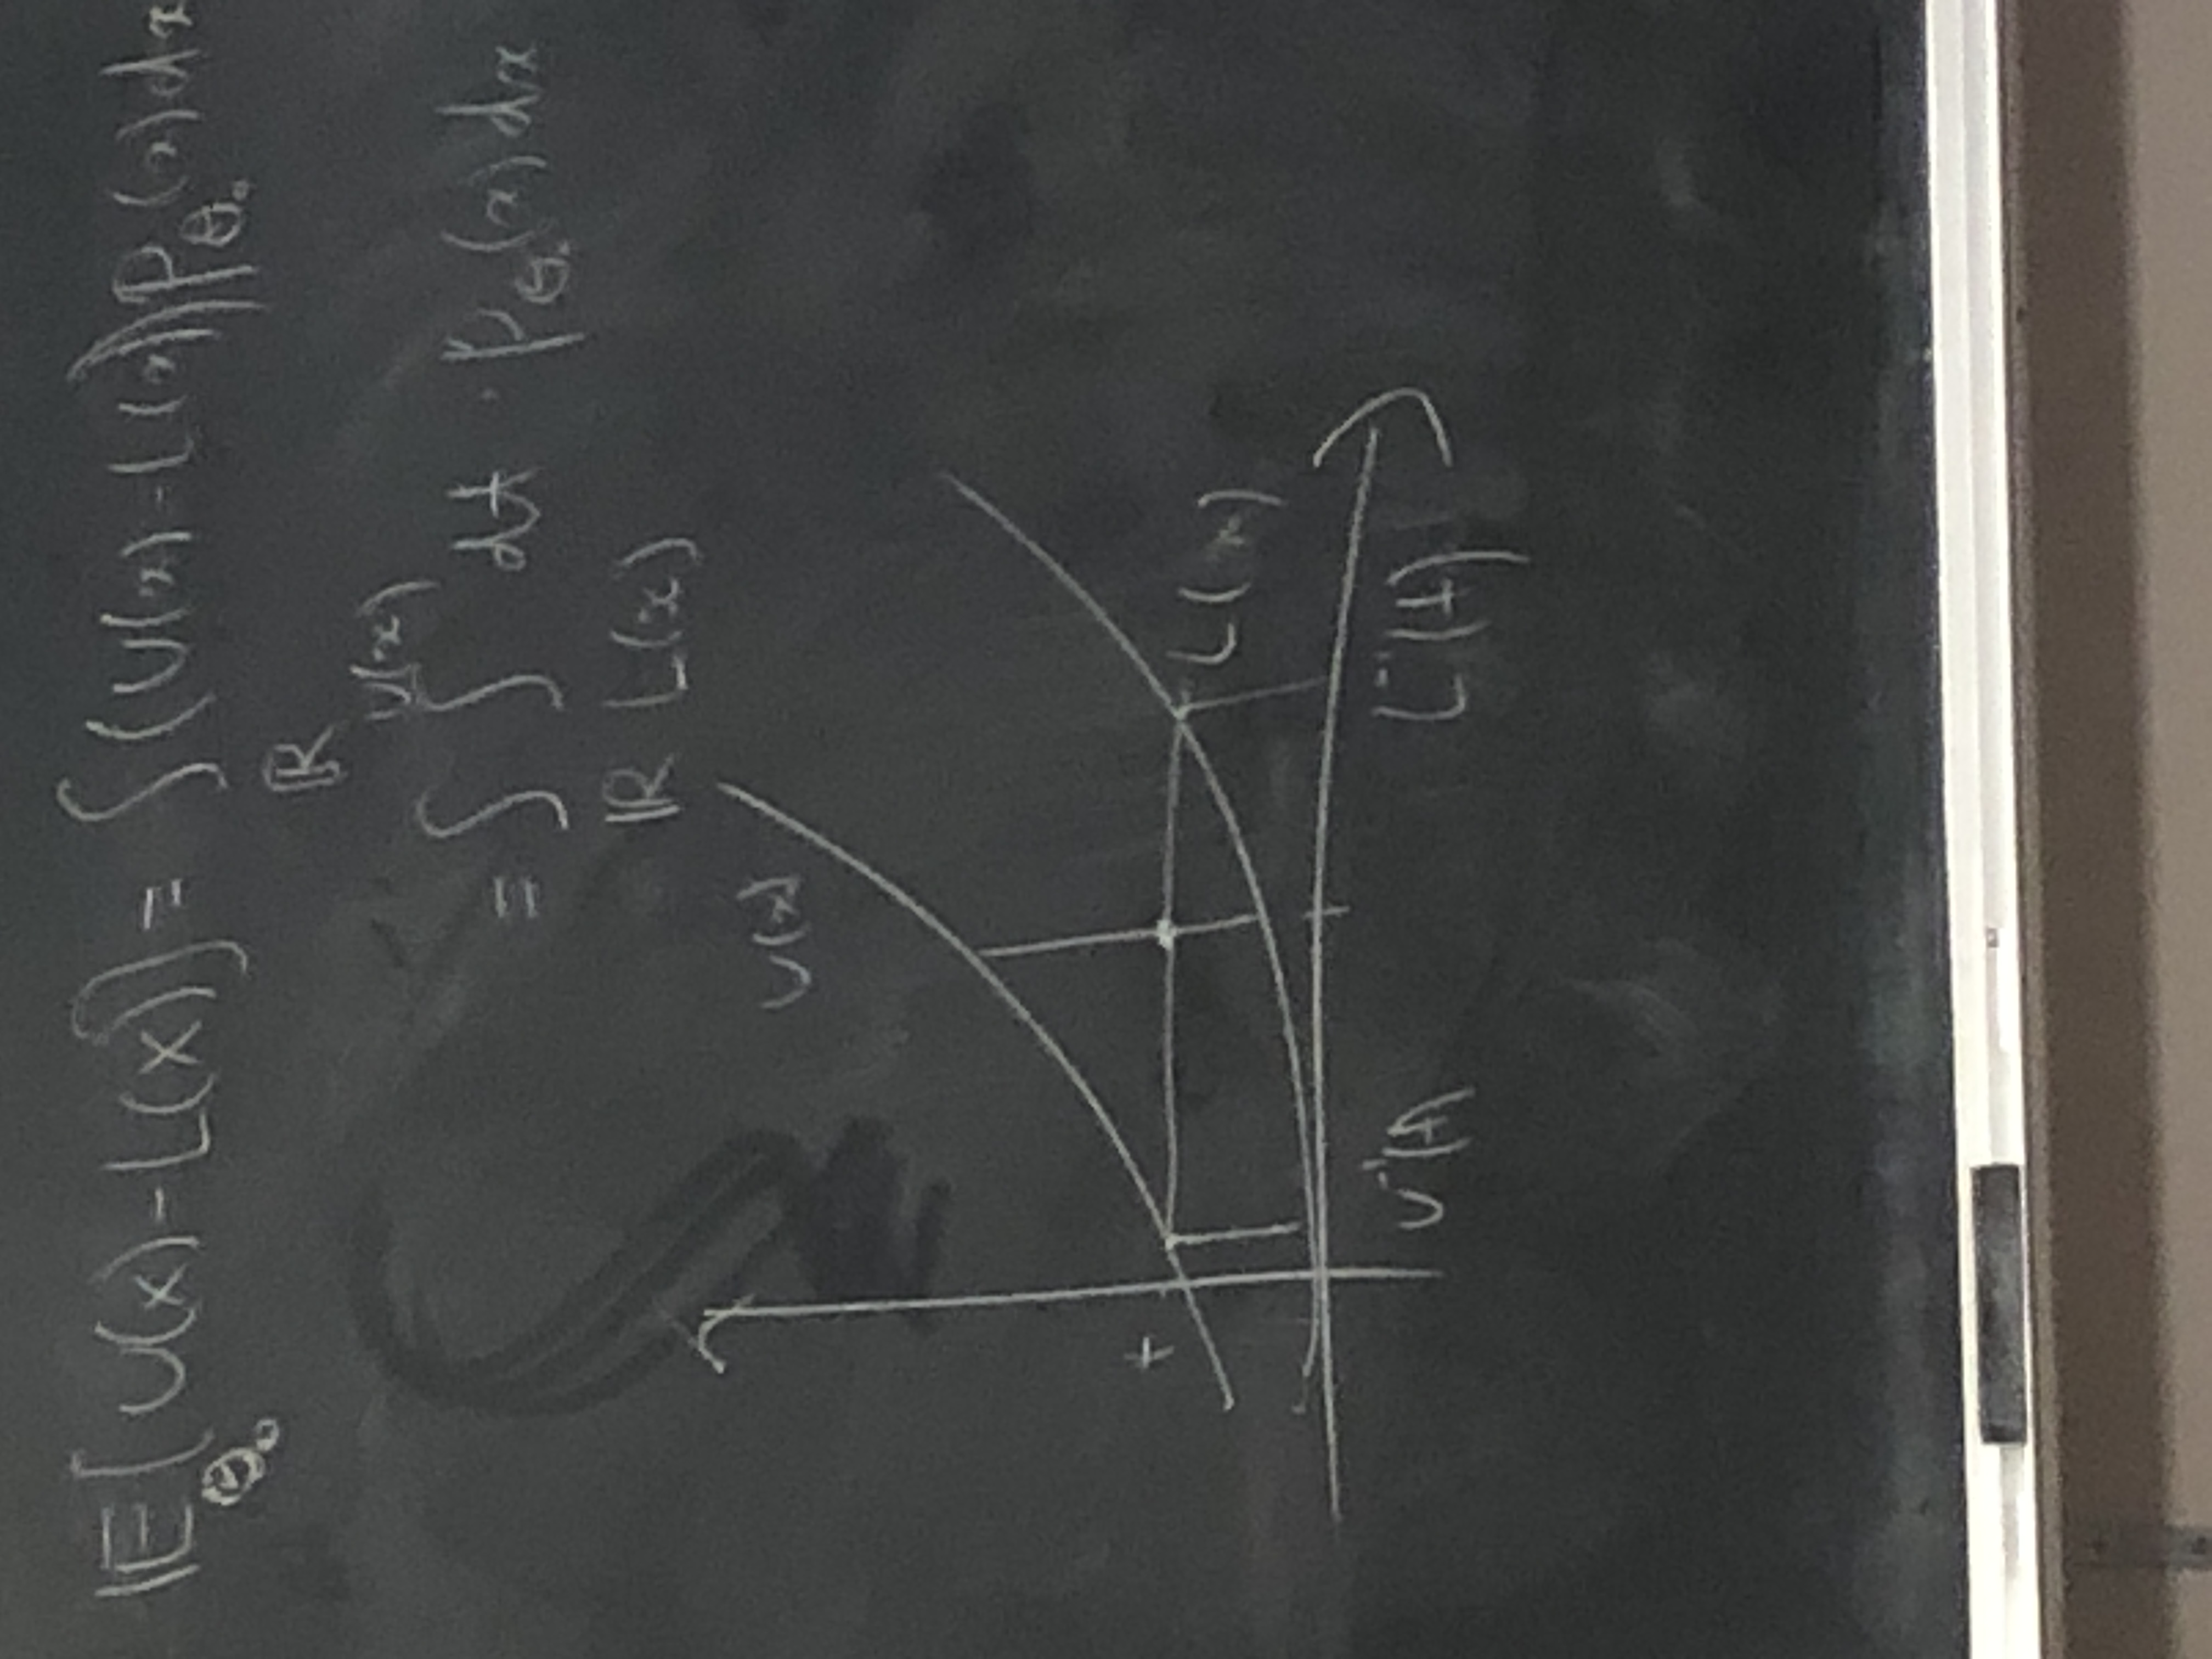
\includegraphics[angle=270,scale=0.1]{mathstats_thm_pratt_img}
\caption{Visual depiction of change of integrands in proof of Theorem \ref{mathstats.thm.pratt}.}
\label{mathstats.fig.pratt.thm.proof}
\end{center}
\end{figure}


\end{proof}

\begin{example}[\textbf{``The Rule of Threes"}]

Suppose \(X_1, \ldots, X_n \sim \operatorname{Ber}(p)\), i.i.d. Assume that \(\sum_{i=1}^n x_i = 0\). Find the \(95\%\) upper confidence bound for \(p\). (it is approximately equal to \(3/n\)). 

\end{example}

\begin{solution}

Consider testing \(H_0: p \geq p_0\) against \(H_a: p < p_0\). We know that \(X = \sum_{i=1}^n X_j\) is a complete sufficient statistic and \(X \sim \operatorname{Binomial}(n, p)\), so \(\mathbb{P}_p (X = x) = \binom{n}{x}p^x(1-p)^{n-x}\), a monotone likelihood ratio with respect to \(T(X) = X\). Therefore the UMP (nonrandomized) test is

\[
\phi^* = \begin{cases}
1, & X \leq c \\
%\gamma, & \\
0, & X > c
\end{cases}
\]

(since this test is nonrandomized, it will only be UMP for specific values of \(\alpha\)) where \(c = c(p_0, \alpha) \in \mathbb{Z}_+\) solves

\[
\alpha = \mathbb{P}(\text{Type I error}) = \mathbb{P}_{p_0}( X \leq c) = \sum_{j=0}^{ c(p_0, \alpha)} \binom{n}{j} p_0^j (1 - p_0)^{n-j} 
\]

To find the \(95\%\) upper confidence bound for \(p\), we want to know for which values of \(p_0\) is 0 in the acceptance region (\(0 \in \operatorname{AR}(p_0)\)). Note that for this hypothesis test with null hypothesis \(p \geq p_0\), the acceptance regions are nested, meaning that \(p_1 < p_2 \implies \{ \text{the rejection region for } p_1\} \subseteq \{\text{the rejection region for } p_2 \} \iff \operatorname{AR}(p_2) \subseteq \operatorname{AR}(p_1)\). Hence we need to find the largest \(p\) such that \(0 \in \operatorname{AR}(p)\). This \(p \) must satisfy

\[
\alpha <  \mathbb{P}_p(X = 0) = \sum_{j=0}^0 \binom{n}{j}p^j(1-p)^{n-j}  \iff (1-p)^n > \alpha \iff p < 1 - \alpha^{1/n}.
\]

Then \(\alpha\) is small implies \(\alpha^{1/n} = e^{\log(\alpha)/n} \approx 1 + \log(\alpha)/n\). Using this, we get \(p < - \log(\alpha)/n\). When \(\alpha = 0.05\), \(- \log(\alpha) = \log (1/0.05) \approx 3\).

\end{solution}

\begin{exercise}

What if we observe 1 success in \(n\) trials? Find an equation for a \((1-\alpha)\) upper confidence bound for \(p\).

\end{exercise}

\section{\(U\)-Statistics}\label{mathstats.sec.u.stats}

\subsection{Basic Definitions and Properties \cite[Sections 5.1 and 5.2]{serfling1980}, \cite[Section 15.1]{dasgupta2008asymptotic}}

While the limiting distribution of linear statistics is known from the canonical Central Limit Theorem (under suitable moment conditions), limiting distributions of nonlinear statistics are more difficult. However, a class of nonlinear statistics called \textbf{\(U\)-Statistics} have a common CLT.

\begin{definition}[\textbf{\(U\)-Statistics; definition drawing from Section 5.1.1 of \citet[p. 190 of pdf, p. 172 of book]{serfling1980} and \citet[Chapter 15, p. 240 of pdf, p. 225 of book]{dasgupta2008asymptotic}}]\label{mathstats.def.u.stat}

Let \(X_1, X_2, \ldots\) be independent observations on a distribution \(F\). (They may be vector-valued, but usually we will consider the real-valued case.) Consider a parametric function \(\theta = \theta(F)\) for which there is an unbiased estimator. That is, \(\theta(F)\) may be represented as

\[
\theta(F) = \mathbb{E}_F\left[h \left(X_1, \ldots, X_m\right) \right] = \int \cdots \int h(x_1, \ldots, x_m) dF(x_1) \ldots dF(x_m)
\]

for some function \(h = h(x_1, \ldots, x_m)\), called a \textbf{kernel}. Without loss of generality, we may assume \(h\) is symmetric\footnote{To see why this is without loss of generality, suppose \(h\) is not symmetric. Then replace \(h\) with the symmetric kernel \((1/m!) \sum_p h(x_{i_1}, \ldots x_{i_m})\) where \(\sum_p\) denotes summation over the \(m!\) permutations \((i_1, \ldots, i_m)\) of \((1, \ldots , m\)).}. Of course, \(h(X_1, \ldots, X_m)\) is an unbiased estimator for \(\theta(F)\), but a better unbiased estimate should exist if \(n > m\) because \(h(X_1, \ldots, X_m)\) does not use all of the sample data.

In particular, for any kernel \(h\), the corresponding \textbf{\(U\)-Statistic of order \(m\) with kernel \(h\)} for estimation of \(\theta\) on the basis of a sample \(X_1, \ldots, X_n\) of size \(n \geq m\) is obtained by averaging the kernel \(h\) symmetrically over the observations:

\[
U_n = U(X_1, \ldots, X_n) := \frac{1}{\binom{n}{m}} \sum_c h(X_{i_1}, \ldots, X_{i_m}),
\]

where \(\sum_c\) denotes summation over the \(\binom{n}{m}\) combinations of \(m\) distinct elements \(\{i_1, \ldots, i_m\}\) from \([n]\). Clearly, \(U_n\) is an unbiased estimate of \(\theta\).

\end{definition}

\begin{example}[\textbf{Example 15.2 in \citet{dasgupta2008asymptotic}}]\label{mathstats.ex.15.2.dasgupta}

Let \(m=2\) and \(h(x_1, x_2) = (x_1 -x_2)^2/2\). One can show that

\[
\frac{1}{\binom{n}{2}} \sum_{i < j} \frac{(X_i -X_j)^2}{2} = \frac{1}{n-1} \sum_{i=1}^n (X_i - \overline{X})^2.
\]

That is, the sample variance is a \(U\)-statistic.

\end{example}

A \(U\)-statistic may be represented as the result of conditioning the kernel on the order statistic; that is, for \(n \geq m\),

\[
U_n = \mathbb{E}\left[ h(X_1, \ldots, X_m) \mid \boldsymbol{X}_{(n)} \right]
\]

where \( \boldsymbol{X}_{(n)}\) denotes the order statistic. This implies that any statistic \(S = S(X_1, \ldots, X_n)\) for unbiased estimation of \(\theta = \theta(F)\) may be improved by the corresponding \(U\)-statistic. 

\begin{theorem}[\textbf{Optimality property of \(U\)-statistics; \citet[Section 5.14, p. 194 of pdf, p. 176 of book]{serfling1980}}]

Let \(S = S(X_1, \ldots, X_n)\) be an unbiased estimator of \(\theta(F)\) based on a sample \(X_1, \ldots, X_n\) from the distribution \(F\). Then the corresponding \(U\)-statistic is also unbiased and

\[
\Var_F(U) \leq \Var_F(S),
\]

with equality if and only if \(\mathbb{P}_F(U = S) = 1\).

\end{theorem}

\begin{proof}

The kernel associated with \(S\) is 

\[
\frac{1}{n!} \sum_p S(x_{i_1}, \ldots, x_{i_n}),
\]

which in this case \(m=n\) is the \(U\)-statistic associated with itself. That is, the \(U\)-statistic associated with \(S\) may be expressed as \(U = \mathbb{E}(S \mid \boldsymbol{X}_{(n)})\). Therefore

\[
 \mathbb{E}_F(U^2) = \mathbb{E}_F\left(\left[\mathbb{E}_F \left(S \mid\boldsymbol{X}_{(n)}\right) \right]^2 \right) \leq  \mathbb{E}_F\left(\mathbb{E}_F \left(S^2 \mid\boldsymbol{X}_{(n)}\right)  \right) = \mathbb{E}_F(S^2),
\]

where the inequality follows from the fact that

\[
\Var_F\left(S \mid \boldsymbol{X}_{(n)} \right) = \mathbb{E}_F \left(S^2 \mid\boldsymbol{X}_{(n)}\right)  - \left[\mathbb{E}_F \left(S \mid\boldsymbol{X}_{(n)}\right) \right]^2  \geq 0.
\]

with equality if and only if \(\mathbb{E}_F(S \mid \boldsymbol{X}_{(n)})\) equals \(S\) with probability 1. Since \(\mathbb{E}_F(U) = \mathbb{E}_F(S)\), the proof is complete.

\end{proof}

\begin{remark}

Since \(\boldsymbol{X}_{(n)}\) is sufficient for any family of distributions containing \(F\), the \(U\)-statistic is the result of conditioning on a sufficient statistic. Therefore this result is simply a special case of the Rao-Blackwell theorem (Theorem \ref{mathstats.thm.rao.blackwell}). This further implies that if \(\boldsymbol{X}_{(n)}\) is complete sufficient then the \(U\)-statistic is the MVUE of \(\theta\) by Lehmann-Scheffe (Theorem \ref{mathstats.lehmann.scheffe}). 

\end{remark}

Next we will find the variance of a \(U\)-statistic. In order to do this, we will establish some notation that will be useful.

\begin{definition}[\textbf{Notation from Section 5.1.5 of \citet{serfling1980}}]


For a symmetric kernel \(h(x_1, \ldots, x_m)\) satisfying \(\E_F| h(X_1, \ldots, X_m)| < \infty\), we define the associated functions

\[
h_c(x_1, \ldots, x_c) := \E_F \left[ h(x_1, \ldots, x_c, X_{c+1}, \ldots, X_m) \right] = \E_F \left[ h(X_1, \ldots,  X_m)  \mid (X_1, \ldots, X_c) = (x_1, \ldots, x_c) \right] 
\]

for each \(c \in [m-1]\), and define \(h_m := h\). Note that for \(1 \leq c \leq m -1\),

\[
h_c(x_1, \ldots, x_c) = \E_F\left[ h_{c+1}(x_1, \ldots, x_c, X_{c+1}) \right].
\]

Recall \(\theta(F) = \E_F[h(X_1, \ldots, X_m)]\). Define

\[
\tilde{h} := h - \theta(F)
\]

and

\[
\tilde{h}_c := h_c - \theta(F), \quad c \in [m].
\]

\end{definition}


\begin{remark}

Note that since by Definition \ref{mathstats.def.u.stat}

\[
U_n = \frac{1}{\binom{n}{m}} \sum_c h(X_{i_1}, \ldots, X_{i_m}),
\]

it holds that

\begin{align}
U_n - \theta  & =  \binom{n}{m}^{-1} \sum_c h(X_{i_1}, \ldots, X_{i_m}) - \binom{n}{m}^{-1} \binom{n}{m} \theta \nonumber
\\  & = \binom{n}{m}^{-1} \sum_c \left[ h(X_{i_1}, \ldots, X_{i_m}) - \theta \right] \nonumber
\\  & = \binom{n}{m}^{-1} \sum_c \tilde{h}(X_{i_1}, \ldots, X_{i_m}). \label{mathstats.u.id.var}
\end{align}

\end{remark}


\begin{definition}[\textbf{From Section 5.2.1 of \citet{serfling1980}}]

Consider a symmetric kernel satisfying \(E_F[ h^2(X_1, \ldots, X_m)] < \infty\). Note that 

\[
\E_F \tilde{h}_c(X_1, \ldots, X_c) = \E_F \left( \E_F \left[ h(x_1, \ldots, x_c, X_{c+1}, \ldots, X_m) \right] - \theta \right)  = 0, \qquad \forall c \in [m].
\]

Define \(\zeta_0 := 0\) and for \(c \in [m]\)

\[
\zeta_c := \Var_F \left[ h_c(X_1, \ldots, X_c) \right] = \E_F \left[ \tilde{h}_c^2(X_1, \ldots, X_c) \right].
\]

\end{definition}

\begin{example}[\textbf{Example A in Section 5.2.1 of \citet{serfling1980}; extension of Example \ref{mathstats.ex.15.2.dasgupta}}]

Again, let \(m=2\) and \(h(x_1, x_2) = (x_1 -x_2)^2/2\). We have already shown in Example \ref{mathstats.ex.15.2.dasgupta} that this \(U\)-statistic corresponds to the sample variance; that is, \( \E_F[h(X_1, X_2)] = \sigma^2(F) =: \theta(F)\). We have

\begin{align*}
\tilde{h}(x_1, x_2) & = h(x_1, x_2) - \sigma^2,
\\ h_1(x) & = \E_F \left[ h(X_1, X_2 )  \mid X_1 = x \right]= \E_F \left[\frac{1}{2}(x - X_2)^2 \right]  = \frac{1}{2}\E_F \left[x^2 - 2xX_2 + X_2^2 \right] 
\\ & = \frac{1}{2}\left(x^2 - 2x\mu + \sigma^2 + \mu^2 \right),
\\ \tilde{h}_1(x) & =\frac{1}{2}\left(x^2 - 2x\mu + \sigma^2 + \mu^2 \right) - \sigma^2 = \frac{1}{2}\left(x^2 - 2x\mu - \sigma^2 + \mu^2 \right) = \frac{1}{2}\left(\left[x - \mu\right]^2 - \sigma^2 \right) ,
\\ \zeta_1 & =\E_F \left[ \tilde{h}_1^2(X_1) \right] =\E_F \left[ \frac{1}{2}\left(\left[X_1 - \mu\right]^2 - \sigma^2 \right)\right]^2 = \frac{1}{4} \Var_F \left[ \left( X_1 - \mu \right)^2 \right] = \frac{1}{4}\left(\mu_4 - \sigma^4\right),
\\ \E (h^2) & = \frac{1}{4}\E \left[ \left(X_1- X_2\right)^2 \right]^2  = \frac{1}{4}\E \left[ \left(X_1 - \mu\right) -\left( X_2 - \mu \right) \right]^4
\\  &= \frac{1}{4}\sum_{j=0}^4 \binom{4}{j} (-1)^{4-j} \E \left[ \left(X_1 - \mu\right)^j \right] \E \left[ \left( X_2 - \mu \right)^{4-j} \right]
 = \frac{1}{4}\left(2 \mu_4 + 6 \sigma^4 \right),
\\ \zeta_2 & =  \E_F \left[ \tilde{h}_2^2(X_1, X_2) \right]   =  \E_F \left[ \left(h(X_1, X_2) - \sigma^2 \right)^2 \right] =  \E_F \left[ h^2(X_1, X_2) - 2 \sigma^2 h(X_1, X_2)  + \sigma^4 \right]
\\&  =  \E_F \left[ h^2(X_1, X_2) \right]  - \sigma^4 =  \frac{1}{4}\left(2 \mu_4 + 6 \sigma^4 \right)  - \sigma^4 = \frac{1}{2} \left( \mu_4 + \sigma^4\right).
\end{align*} 

\end{example}

\begin{proposition}[\textbf{Problem 5.P.3(i) in \citet{serfling1980}}]

\[
0 = \zeta_0 \leq \zeta_1 \leq \ldots \leq \zeta_m = \Var_F(h) < \infty.
\]

\end{proposition}

\begin{proposition}[\textbf{Problem 5.P.4 in \citet{serfling1980}}]\label{mathstats.prop.5.p.4}

Consider two sets \(\{a_1, \ldots, a_m\} \subset [n]\) and \(\{b_1, \ldots, b_m\} \subset [n]\) of distinct integers. Let \(c = \left|\{a_1, \ldots, a_m\} \cap \{b_1, \ldots, b_m\}  \right| \) be the number of integers common to both. Then by symmetry of \(\tilde{h}\) and independence of \(\{X_1, \ldots, X_n\}\),

\[
\E_F \left[ \tilde{h}(X_{a_1}, \ldots, X_{a_m}) \tilde{h}(X_{b_1}, \ldots, X_{b_m})  \right] = \zeta_c.
\]

\end{proposition}

\begin{remark}

Note also that the number of distinct choices for two such sets having exactly \(c\) elements in common is \(\binom{n}{m} \binom{m}{c} \binom{n-m}{m-c}\). Also, since \(\E_F \tilde{h} = 0\), we have that

\[
\zeta_c = \Cov \left( \tilde{h}(X_{a_1}, \ldots, X_{a_m}), \tilde{h}(X_{b_1}, \ldots, X_{b_m}) \right) 
%\\ & = \Cov \left( \tilde{h}(X_{a_1}, \ldots, X_{a_m}), \tilde{h}(X_{b_1}, \ldots, X_{b_m}) \right)
%\\ & = \Cov \left( h(X_{a_1}, \ldots, X_{a_m}), h(X_{b_1}, \ldots, X_{b_m}) \right)
 = \Cov \left( h(X_{a_1}, \ldots, X_{a_m}), h(X_{b_1}, \ldots, X_{b_m}) \right)
\]

\[
h_c(x_1, \ldots, x_c) = \E_F\left[ h_{c+1}(x_1, \ldots, x_c, X_{c+1}) \right].
\]

\end{remark}

Now we can find the variance of a \(U\)-statistic. We have

\begin{align}
\Var_F(U_n) & = \E_F \left[ (U_n - \theta)^2\right] \nonumber
\\ \text{(using \eqref{mathstats.u.id.var})} \qquad & = \E_F \left[ \left(  \binom{n}{m}^{-1} \sum_c \tilde{h}(X_{i_1}, \ldots, X_{i_m}) \right)^2\right]  \nonumber
\\ & =  \binom{n}{m}^{-2}  \sum_c  \sum_c \E_F \left[ \tilde{h}(X_{a_1}, \ldots, X_{a_m}) \tilde{h}(X_{b_1}, \ldots, X_{b_m}) \right]  \nonumber
\\ \text{(by Proposition \ref{mathstats.prop.5.p.4})} \qquad & =  \binom{n}{m}^{-2}  \sum_{c=0}^n \binom{n}{m} \binom{m}{c} \binom{n-m}{m-c} \zeta_c   \nonumber
\\ \text{(using \(\zeta_0 = 0\))} \qquad & =  \binom{n}{m}^{-1}  \sum_{c=1}^n \binom{m}{c} \binom{n-m}{m-c} \zeta_c . \label{mathstats.u.var}
\end{align}


\begin{lemma}[\textbf{Lemma A in Section 5.2.1 of \citet{serfling1980}}]

The variance of \(U_n\) is given by \eqref{mathstats.u.var} and satisfies

\begin{enumerate}[(i)]

\item

\[
\frac{m^2}{n} \zeta_1 \leq \Var_F(U_n) \leq \frac{m}{n} \zeta_m,
\]


\item

\[
(n+1)\Var_F(U_{n+1}) \leq n \Var_F(U_n), \qquad \text{and}
\]

\item

\[
\Var_F(U_n) = \frac{m^2 \zeta_1}{n} + \mathcal{O}(n^{-2}), \qquad n \to \infty.
\]

\end{enumerate}

\end{lemma}

\subsection{Asymptotics \cite[Section 5.3]{serfling1980}, \cite[Section 15.2]{dasgupta2008asymptotic}}


Asymptotic theory for \(U\)-statistics is not straightforward since the summands are in general dependent. Hajek had the idea of projecting \(U\) onto the class of linear statistics of the form \(n^{-1} \sum_{i=1}^n h(X_i)\). It turns out that the projection is the dominant part and determines the limiting distribution of \(U\). 

\begin{definition}[\textbf{Hajek projection; Definition from \citet[Section 5.3.1, p. 206 of pdf, p. 188 of book]{serfling1980} and \citet[Section 3.3]{Wager2018}}]

Assume \(\E_F |h| < \infty\). Then the \textbf{Hajek projection} of the \(U\)-statistic \(U_n\) is defined as 

\[
\hat{U}_n :=  \theta + \sum_{i=1}^n \left( \E_F[U_n \mid X_i ]  - \theta \right) =\sum_{i=1}^n \E_F\left[ U_n \mid X_i \right] - (n-1) \theta
\]

Note that it is a sum of i.i.d. random variables. In terms of the function \(\tilde{h}_1\), we have

\[
\hat{U}_n  = \theta + \frac{m}{n} \sum_{i=1}^n \tilde{h}_1(X_i).
\]

\end{definition}

\citet{dasgupta2008asymptotic} uses a slightly different convention to define \(U\) statistics (their definition projects \(U - \theta\) rather than \(U\), so their definition equals the above definition minus \(\theta\)).

\begin{definition}[\textbf{Hajek projection; Definition 15.2 in \citet{dasgupta2008asymptotic}}]

The \textbf{Hajek projection} of \(U - \theta\) onto the class of statistics \(\sum_{i=1}^n h(X_i)\) is

\[
\hat{U} = \hat{U}_n = \sum_{i=1}^n \mathbb{E}_F(U - \theta \mid X_i) .
\]


\end{definition}

\begin{theorem}[\textbf{Theorem 15.1 in \citet{dasgupta2008asymptotic}}]

Suppose the kernel \(h\) is twice integrable; i.e., \(\E h^2 < \infty\). Then

\[
\sqrt{n}(U - \hat{U}) \xrightarrow{p} 0
\]

and

\[
\sqrt{n}(U - \theta) \xrightarrow{D} \mathcal{N}(0, m^2 \zeta_1).
\]

\end{theorem}

\begin{definition}[\textbf{Definition 6 in \citet{Wager2018}}]

\(U\) is \textbf{\(\nu(s)\)-incremental} if 

\[
\frac{\Var\left[ \hat{U} \right]}{\Var\left[ U \right]} \gtrsim \nu(s),
\]

where

\[
f(s) \gtrsim  g(s) \qquad \iff \qquad \underset{s \to \infty}{\lim \inf} \left( \frac{f(s)}{g(s)} \right) \geq 1.
\]

(That is, \(U\) is \(\nu(s)\)-incremental if 

\[
 \underset{s \to \infty}{\lim \inf} \left( \frac{\Var\left[ \hat{U} \right] / \Var\left[ U \right]}{\nu(s)} \right) \geq 1.)
 \]

\end{definition}

%\begin{remark}
%It can be shown that \(\hat{U} = \frac{m}{n} \sum_{i=1}^n \tilde{h}_1(X_i)\), where 
%
%\[
%\tilde{h}_1(x) := \mathbb{E}(h(X_1, \ldots, X_m) \mid X_1 = x) - \theta.
%\]
%
%Let
%
%\[
%h_1(x) := \mathbb{E}(h(X_1, \ldots, X_m) \mid X_1 = x)
%\]
%
%so that
%
%\[
%\tilde{h}_1 = h_1 - \theta(F).
%\]
%
%\end{remark}

\section{Influence Functions (Section 6.6.1 of \citet{serfling1980})}

\section{\(M\)-Estimators (Chapter 7 of \citet{serfling1980})}

Many estimation methods are based on minimization of some function of the observations \(\{X_i\}\) and the unknown parameter \(\theta\), e.g. the least squares estimator

\[
 \hat{\theta} = \underset{\theta}{\arg \min} \left\{ d(\theta; X_1, \ldots, X_n) \right\} = \underset{\theta}{\arg \min} \left\{  \sum_{i=1}^n (X_i - \theta)^2 \right\}.
\]

Similarly, the least absolute values estimator of \(\theta\) is given by

\[
 \hat{\theta} = \underset{\theta}{\arg \min} \left\{  \sum_{i=1}^n |X_i - \theta| \right\}.
\]

Maximum likelihood estimation may be regarded as an approach of this type as well. Typically the problem of minimizing a function of data and a parameter reduces to a problem involving solving a system of equations for an estimator \(\hat{\theta}\). Statistics given as solutions of equations are called \textbf{M-statistics.} 

\section{Distance Correlation}


%\bibliographystyle{abbrvnat}
%\bibliography{mybib2fin}
%\end{document}







